%% Copyright 2007-2024 Elsevier Ltd 
%% This file is part of the 'Elsarticle Bundle'.
%% ---------------------------------------------
%% It may be distributed under the conditions of the LaTeX Project Public
%% License, either version 1.3 of this license or (at your option) any
%% later version.  The latest version of this license is in
%%    http://www.latex-project.org/lppl.txt
%% and version 1.3 or later is part of all distributions of LaTeX
%% version 1999/12/01 or later.
%% The list of all files belonging to the 'Elsarticle Bundle' is
%% given in the file `manifest.txt'.
%% Template article for Elsevier's document class `elsarticle'
%% with numbered style bibliographic references
%% SP 2008/03/01
%% $Id: elsarticle-template-num.tex 249 2024-04-06 10:51:24Z rishi $
\documentclass[preprint, 12pt]{elsarticle}

%% Use the option review to obtain double line spacing
%% \documentclass[authoryear,preprint,review,12pt]{elsarticle}

%% Use the options 1p,twocolumn; 3p; 3p,twocolumn; 5p; or 5p,twocolumn
%% for a journal layout:
%% \documentclass[final,1p,times]{elsarticle}
%% \documentclass[final,1p,times,twocolumn]{elsarticle}
%% \documentclass[final,3p,times]{elsarticle}
%% \documentclass[final,3p,times,twocolumn]{elsarticle}
%% \documentclass[final,5p,times]{elsarticle}
%% \documentclass[final,5p,times,twocolumn]{elsarticle}

%% For including figures, graphicx.sty has been loaded in
%% elsarticle.cls. If you prefer to use the old commands
%% please give \usepackage{epsfig}

%% The amssymb package provides various useful mathematical symbols
\usepackage{amssymb}
%% The amsmath package provides various useful equation environments.
\usepackage{natbib}
\usepackage{amsmath}
\usepackage{multicol,multirow}
\usepackage{tikz}
\usepackage{rotating}
\usepackage{anyfontsize}
\usepackage{subcaption}
\usepackage{algorithm, algorithmicx, algpseudocode}
% \usepackage[authoryear]{natbib}

%% The amsthm package provides extended theorem environments
%% \usepackage{amsthm}
\usepackage{amsthm}

%% The lineno packages adds line numbers. Start line numbering with
%% \begin{linenumbers}, end it with \end{linenumbers}. Or switch it on
%% for the whole article with \linenumbers.
%% \usepackage{lineno}

\journal{Non-Newtonian Fluid Mechanics}


\begin{document}

\begin{frontmatter}

%% Title, authors and addresses

%% use the tnoteref command within \title for footnotes;
%% use the tnotetext command for theassociated footnote;
%% use the fnref command within \author or \affiliation for footnotes;
%% use the fntext command for theassociated footnote;
%% use the corref command within \author for corresponding author footnotes;
%% use the cortext command for theassociated footnote;
%% use the ead command for the email address,
%% and the form \ead[url] for the home page:
%% \title{Title\tnoteref{label1}}
%% \tnotetext[label1]{}
%% \author{Name\corref{cor1}\fnref{label2}}
%% \ead{email address}
%% \ead[url]{home page}
%% \fntext[label2]{}
%% \cortext[cor1]{}
%% \affiliation{organization={},
%%             addressline={},
%%             city={},
%%             postcode={},
%%             state={},
%%             country={}}
%% \fntext[label3]{}

\title{{\color{red} Verification of an Incompressible Viscoelastic Flow Solver Using the Method of Manufactured Solutions for Oldroyd-B and Giesekus Constitutive Models}}

%% use optional labels to link authors explicitly to addresses:
%% \author[label1,label2]{}
%% \affiliation[label1]{organization={},
%%             addressline={},
%%             city={},
%%             postcode={},
%%             state={},
%%             country={}}
%%
%% \affiliation[label2]{organization={},
%%             addressline={},
%%             city={},
%%             postcode={},
%%             state={},
%%             country={}}

\author[1]{Juniormar Organista}
\author[1]{Leandro F. de Souza}
\author[2,3]{Célio Fernandes}
\author[1]{Welton L. Costa}
\author[1]{Aquisson T. G. da Silva}
\author[1]{Antonio Castelo}

%% Author affiliation
\affiliation[1]{organization={Institute of Mathematical and Computer Sciences (ICMC), University of São Paulo (USP)},
            addressline={Av. Trab. São Carlense, 400 - Centro}, 
            city={São Carlos},
            postcode={13566-590}, 
            state={SP},
            country={Brazil}
            }
\affiliation[2]{organization={Transport Phenomena Research Center (CEFT), Department of Mechanical Engineering, Faculty of Engineering, University of Porto (FEUP)},
            addressline={Rua Dr. Roberto Frias s/n}, 
            postcode={4200-465}, 
            state={Porto},
            country={Portugal}
            }
\affiliation[3]{organization={Center of Mathematics (CMAT), University of Minho},
            addressline={Campus of Gualtar}, 
            postcode={4710–057}, 
            state={Braga},
            country={Portugal}
            }
%% Abstract
\begin{abstract}
	{\color{red} This study introduces an innovative application of the Method of Manufactured Solutions (MMS) to validate high-order compact finite-difference schemes for solving two-dimensional incompressible viscoelastic flows in the vorticity-stream function formulation. Using the lid-driven cavity flow as a benchmark, the MMS generates artificial analytical solutions that retain the original equations and boundary conditions, enabling rigorous assessment of numerical accuracy, convergence, and stability. The approach is tested on two constitutive models—Oldroyd-B and Giesekus—across Reynolds numbers ($1 \leq Re \leq 1000$), solvent viscosity ratios ($\beta_{nn}$ = 0.1–1.0), and, for the Giesekus constitutive model, mobility parameters ($\alpha_G$ = 0.1–0.5), with a fixed Weissenberg number. Results demonstrate a convergence order of approximately 4.5 for most variables, though vorticity exhibits slightly lower orders at higher Reynolds numbers. Mesh refinement consistently reduces errors, confirming the method’s robustness across parameters and constitutive models. The study underscores the MMS as a powerful tool for verifying complex viscoelastic flow simulations and provides comprehensive data to ensure reproducibility and future applicability.}
\end{abstract}

%%Graphical abstract
%\begin{graphicalabstract}
%\includegraphics{grabs}
%\end{graphicalabstract}

%% Keywords
\begin{keyword}
Viscoelastic Fluids \sep High-order Numerical Method \sep Code Verification \sep Method of Manufactured Solutions \sep Cavity Flow.
\end{keyword}

\end{frontmatter}


%%%%%%%%%%%%%%%%%%%%%%%%%%%%%%%%%%%%%%%%%%
\section{Introduction}
\label{sec:Introduction}

Code verification plays a crucial role in computational modelling, as it
provides a way to assess the accuracy and reliability of numerical codes that
are used to simulate complex physical phenomena \cite{Khoshghalb2019,
Tranquilli2022}. The verification process involves comparing the numerical
results obtained from the code with known analytical solutions or benchmark
cases where the solution is already established \cite{Fernandes2018,
Pedro2020}. By conducting code verification, researchers can ensure that their
computational codes are correctly implemented and capable of producing accurate
results. This verification process is essential for establishing confidence in
the code's ability to accurately capture the physics of the problem under
investigation. It helps identify and rectify errors or inconsistencies in the
code implementation, ensuring that numerical simulations yield reliable and
trustworthy results. Code verification also helps identify limitations of the
numerical methods used and guides the development of more robust and accurate
algorithms. 

The Method of Manufactured Solutions (MMS) is a powerful tool used to verify
codes in computational modelling \cite{Roy2004, Habla2016, Muralha2020,
Freno2021}. In the MMS, an analytical solution with known properties is
specifically manufactured for a given problem. This manufactured solution
incorporates the same mathematical equations and boundary conditions as the
problem being simulated. When the manufactured solution is solved using the
numerical code, the accuracy and convergence of the code can be assessed. The
key advantage of the MMS is its ability to generate solutions with known exact
values, allowing a quantitative comparison between the numerical results and
the manufactured solution. Discrepancies between the two can highlight errors
or limitations in the code, such as numerical instabilities or implementation
inaccuracies. The use of the MMS in code verification provides a rigorous and
systematic approach to assess the fidelity of computational codes, ensuring
that they are capable of accurately capturing the physics of the problem. This
process not only instils confidence in the code's reliability but also guides
code developers in identifying and addressing potential weaknesses, leading to
improved accuracy and robustness in computational modelling.

The MMS can play a crucial role in the verification and validation of
computational codes for viscoelastic fluid flow calculations \cite{Garcia2022}.
Viscoelastic fluids exhibit complex rheological behaviours, making their
accurate numerical simulation challenging \cite{Fernandes2017}.
\citeauthor{Tseng2021} studied transient stress overshoot for polymer melts
under start-up shear flow. The ability of the White-Metzner constitutive
equation to analyse the pronounced stress overshoot change at high Weissenberg
numbers was studied. Furthermore, the numerical predictions of the shear stress
growth coefficient at various shear rates demonstrated good agreement with the
experimental data, providing validation for their model. \citet{Pimenta2019}
reported the implementation of coupled solvers for transient- and steady-state
electrically driven viscoelastic flow simulations in the finite-volume
framework. In their work, it was concluded that the coupled solvers are more
accurate in transient simulations and allow the use of larger time steps
without numerical divergence. \citet{Fernandes2022} developed a fully implicit
coupled method for the solution of laminar, incompressible, non-isothermal,
viscoelastic flows based on the log-conformation tensor framework for
high-Weissenberg number problems. The newly developed algorithm was validated
through its application to the non-isothermal viscoelastic matrix-based
Oldroyd-B fluid flow in a benchmark problem involving a two-dimensional
axisymmetric 4:1 planar sudden-contraction geometry. Another widely used
benchmark problem is the flow in the lid-driven cavity, which involves the
translation of the top wall (lid), inducing 2D fluid motion in a quadrangular
channel \cite{Shankar2000}. The flow in the lid-driven cavity is frequently
used for the validation of novel numerical methods and techniques.
\citet{Abuga2020} used the lid-driven cavity to present both validation results
and new benchmark results obtained from their second-order finite-volume-based
OpenFOAM numerical solver for fluid flow governed by the Rolie-Poly
viscoelastic constitutive model. \citet{Fernandes2019} used the lid-driven
cavity flow to study the performance of their second-order fully coupled
numerical algorithm for the solution of laminar incompressible viscoelastic
flows in collocated grids. \citet{Tomio2020} also used the lid-driven cavity
flow to validate their newly developed numerical scheme for viscoelastic fluid
flow calculations, which utilized a second-order fully implicit finite
difference approximation to discretize the convection and diffusion terms
present in the governing equations.

High-order discretization schemes are necessary for studying problems in
computational modelling because they offer several distinct advantages over
traditional low-order methods (first and second orders). High-order schemes
increase accuracy, allowing for more precise and reliable solutions to complex
problems. These methods can capture fine-scale features and gradients more
effectively, reducing numerical errors and mitigating issues related to
numerical dissipation and dispersion. \citet{Souza2005} investigated the
performance of different finite difference schemes in simulating instability
waves within a given flow field. The numerical simulations were based on the
solution of the two-dimensional incompressible flow equations represented in
the vorticity–stream function formulation. Four distinct space discretization
schemes were examined: second-order central differences, fourth-order central
differences, fourth-order compact scheme, and sixth-order compact scheme. Time
integration was achieved using the classic fourth-order Runge–Kutta scheme. The
comparison between these schemes allowed for a comprehensive assessment of
their accuracy and suitability for capturing instability phenomena in the flow.
\citet{Cueto2006} presented a novel approach that utilizes moving least squares
(MLS) approximations to develop high-order finite-volume discretizations. The
proposed methodology is specifically applied to construct numerical schemes for
the shallow water equations on unstructured grids. By employing this mesh-free
technique, they achieve a robust and versatile approximation framework that not
only ensures high-order accuracy but also enables accurate computation of the
viscous fluxes. \citet{Silva2010} presented the results of a verification test
conducted on a Direct Numerical Simulation (DNS) code, which employed a mixed
high-order accuracy, using the MMS. The primary objective of their numerical
code was to simulate the temporal evolution of instability waves in a plane
Poiseuille flow. To achieve this, they solved the governing equations using a
vorticity-stream function formulation for a two-dimensional incompressible
flow. The code employed two distinct numerical schemes: one based on mixed
high-order compact and non-compact finite differences, ranging from fourth to
sixth-order accuracy, and the other utilizing spectral methods for the periodic
streamwise direction. For their verification test, a new analytical solution
was derived that reproduces the accurate characteristics of an instability wave
in a nonlinear stage. \citet{Fadel2011} developed a novel high-order approach
to solve the incompressible Stokes and Navier-Stokes equations. The scheme was
based on a velocity-pressure gradient formulation, offering several advantages:
(i) the application of high-order finite difference stencils on non-staggered
grids, (ii) the utilization of standard Padé schemes for high-order pressure
gradient approximations, and (iii) the seamless incorporation of various
boundary conditions. In their work, detailed results for a range of
two-dimensional steady-state test problems were presented, including Stokes,
Kovasznay, lid-driven cavity, and backward-facing step flows. A fourth-order
scheme was used to demonstrate the accuracy and robustness of the proposed
methods, highlighting the effectiveness of the new high-order approach in
achieving accurate and reliable solutions for a variety of challenging fluid
flow problems. \citet{ZHANG2019634}  proposed a high-order numerical scheme for
the reinitialization of the interface-preserving level set method. The
effectiveness of the method was studied through two-dimensional test cases,
showing its superior properties in terms of accuracy, long-term stability,
interface preservation, and seamless treatment of contact lines. In addition,
results on the pinch-off process of a pendant drop, where topological changes
of the fluid interface are involved, were presented. The proposed approach
proved to be highly reliable and efficient in capturing intricate interface
dynamics. \citet{ALMUSHAIRA2021235} introduced a fast and stable high-order
numerical method designed to solve fractional-in-space reaction-diffusion
equations. Their approach was explicitly based on the fourth-order compact
finite difference scheme, along with the matrix transfer technique (MTT) in
space, employing a Fast Fourier Transform (FFT)-based implementation. Time
integration was achieved using the modified fourth-order Runge-Kutta scheme. To
showcase the performance of their proposed method, they conducted linear
stability analysis and various numerical experiments, including two-dimensional
Fitzhugh-Nagumo, Allen-Cahn \citep{Allen1972}, Gierer-Meinhardt
\citep{Gierer1972}, Gray-Scott \citep{Gray1984}, and three-dimensional
Schnakenberg models \citep{Schnakenberg1979}. The results obtained demonstrate
the accuracy, efficiency, and stability of their approach, establishing its
suitability for solving complex fractional reaction-diffusion problems.

{\color{red} Although higher-order numerical schemes—such as spectral,
finite-di\-ffe\-ren\-ce, and finite element methods—have been extensively
applied in viscoelastic flow simulations, the combined use of a compact
fourth-order finite-difference formulation with systematic verification via the
Method of Manufactured Solutions (MMS) remains underexplored. This study
addresses that gap by applying high-order compact finite-difference schemes to
the two-dimensional incompressible viscoelastic flow equations, formulated in
terms of the flow vorticity function. Verification is performed using MMS for
both the Oldroyd-B and Giesekus constitutive models, with the lid-driven cavity
flow serving as a benchmark case. The proposed approach demonstrates superior
numerical accuracy compared to existing methods, highlighting its effectiveness
and contribution to advancing high-fidelity viscoelastic fluid simulations.

The present study adopts the vorticity-stream function formulation for modeling
two-dimensional incompressible viscoelastic flows. This choice is motivated by
several factors. First, the formulation inherently satisfies the
incompressibility constraint, thereby eliminating the need to solve a pressure
Poisson equation. Second, it avoids the pressure-velocity decoupling
instabilities (such as the so-called chequerboard modes) that can arise in
high-order collocated schemes based on the primitive variables. These
characteristics are particularly attractive in the context of high-order
discretizations.

Despite these benefits, the vorticity-stream function formulation has
well-documented limitations. It is inherently two-dimensional and poses
difficulties in accurately enforcing vorticity boundary conditions, which are
not directly prescribed by the physical problem.

This formulation thus provides a numerically stable and computationally
efficient framework for code verification in two-dimensional viscoelastic
flows, while acknowledging its constraints in broader contexts.}

The paper is organized as follows: Section \ref{sec_MathematicalModel} presents
the governing equations for viscoelastic flows, including the vorticity-stream
function formulation and the constitutive models used, namely Oldroyd-B and
Giesekus. Section \ref{sec_NumericalMethod} describes the high-order compact
finite-difference schemes employed for spatial and temporal discretizations,
along with details of the numerical implementation. Section
\ref{sec_CodeVerification} discusses the method of manufactured solutions (MMS)
used for code verification, explaining how artificial analytical solutions were
constructed and how the precision, stability, and convergence of the numerical
method were evaluated. Section \ref{sec_Results} presents the numerical
results, focusing on the verification of the High-order numerical method
through the benchmark case of the lid-driven cavity flow and providing an
analysis of convergence and error reduction for various parameters, such as
Reynolds numbers, solvent viscosity ratios, and anisotropy of the stress
tensor. Section \ref{sec_Conclusions} summarizes the main findings and suggests
directions for future research in the simulation of viscoelastic fluid flows
using high-order numerical methods.

%%%%%%%%%%%%%%%%%%%%%%%%%%%%%%%%%%%%%%%%%%
\section{Mathematical Model}\label{sec_MathematicalModel}
\unskip

The flow examined in this study is characterized as time-dependent,
two-dimensional, non-Newtonian, incompressible, and isothermal. The governing
equations encompass the continuity equation, which accounts for mass
conservation, the Cauchy equation, which addresses momentum conservation, and a
constitutive equation to determine the non-Newtonian extra-stress tensor. The
dimensionless form of the continuity equation is given by:

\begin{equation}
    \nabla\cdot\mathbf{u} = 0,\label{eq_conservation}
\end{equation}
and the dimensionless momentum equation is expressed as follows:
\begin{equation}
    \dfrac{\partial\mathbf{u}}{\partial t} + \nabla\cdot(\mathbf{uu}) = -\nabla p + \dfrac{\beta_{nn}}{\operatorname{Re}}\nabla^{2}\mathbf{u} + \nabla\cdot\mathbf{T},\label{eq_momentun}
\end{equation}
where $\mathbf{u}$ represents the fluid velocity field, $t$ denotes the time,
$p$ is the pressure in the fluid, and $\beta_{nn} = \eta_{s}/\eta_{0}$ is the
solvent viscosity ratio, where $\eta_{0} = \eta_{s} + \eta_{p}$ is the zero
shear-rate viscosity also called the total viscosity combining both solvent
($\eta_{s}$) and polymeric ($\eta_{p}$) viscosities. Furthermore,
$\operatorname{Re} = (\rho U L)/\eta_{0}$ characterizes the Reynolds number,
where $\rho$ denotes the fluid density, $U$ is the characteristic velocity
scale, and $L$ represents the characteristic length scale (e.g., channel width
for the lid-driven cavity flow). Lastly, $\mathbf{T}$ stands for the symmetric
non-Newtonian extra-stress tensor, which must adhere to an appropriate
constitutive equation, such as the Giesekus viscoelastic constitutive model,
given by:

\begin{align}
    \mathbf{T} + Wi\left[ \dfrac{\partial\mathbf{T}}{\partial t} + \nabla\cdot(\mathbf{uT}) - \nabla\mathbf{u}\cdot\mathbf{T} - \mathbf{T}\cdot\nabla\mathbf{u}^{T} \right] 
    + \nonumber\\ + \dfrac{\alpha_{G}\operatorname{Re}\operatorname{Wi}}{1-\beta_{nn}}\left( \mathbf{T}\cdot\mathbf{T} \right) = 2\dfrac{1-\beta_{nn}}{\operatorname{Re}}\mathbf{D},\label{eq_geral_tensors}
\end{align}
where $\mathbf{D} = \frac{1}{2}\left( \nabla\mathbf{u} + \nabla\mathbf{u}^{T}
\right)$ is the rate of deformation tensor, $\operatorname{Wi} = \lambda U / L$
is the Weissenberg number, with $\lambda$ being the relaxation-time of the
fluid, and $\alpha_{G}$ is the so-called mobility or anisotropy parameter
$(0\leq \alpha_{G}\leq 1)$ being a rheological characteristic of the Giesekus
viscoelastic constitutive model, controlling the shear-thinning viscoelastic
behaviour.

In the two-dimensional case,
Equations~\eqref{eq_conservation}--\eqref{eq_geral_tensors} can be written in
component form as follows:

\begin{align}
    \frac{\partial u}{\partial x}+\frac{\partial v}{\partial y}&=0,\label{cont_bidime}
\end{align}
\begin{subequations}
\begin{align}
    \frac{\partial u}{\partial t}+\frac{\partial(u u)}{\partial x}+\frac{\partial(u v)}{\partial y} &= -\frac{\partial p}{\partial x}+\frac{\beta_{nn}}{\operatorname{Re}}\left(\frac{\partial^2 u}{\partial x^2}+\frac{\partial^2 u}{\partial y^2}\right)+\frac{\partial T_{x x}}{\partial x}+\frac{\partial T_{x y}}{\partial y},\label{movi_x_bidime} \\[7mm]
    \frac{\partial v}{\partial t} + \frac{\partial(u v)}{\partial x} + \frac{\partial(v v)}{\partial y} &= -\frac{\partial p}{\partial y}+\frac{\beta_{nn}}{\operatorname{Re}}\left(\frac{\partial^2 v}{\partial x^2}+\frac{\partial^2 v}{\partial y^2}\right)+\frac{\partial T_{x y}}{\partial x}+\frac{\partial T_{yy}}{\partial y},\label{movi_y_bidime}
\end{align}
\end{subequations}
\begin{subequations}
\begin{align}
    T_{xx} + \operatorname{Wi}\left[\frac{\partial T_{xx}}{\partial t} + \frac{\partial (uT_{xx})}{\partial x} + \frac{\partial (vT_{xx})}{\partial y} - 2T_{xx}\frac{\partial u}{\partial x} - 2T_{xy}\frac{\partial u}{\partial y}\right] + \nonumber\\ + \frac{\alpha_{G}\operatorname{Wi}\operatorname{Re}}{1 - \beta_{nn}}\left(T_{xx}^{2} + T_{xy}^{2}\right) = 2 \frac{1 - \beta_{nn}}{\operatorname{Re}}\frac{\partial u}{\partial x},\label{eq_gies_txx}\\[7mm]
    T_{xy} + \operatorname{Wi}\left[\frac{\partial T_{xy}}{\partial t} + \frac{\partial (uT_{xy})} {\partial x} + \frac{\partial (vT_{xy})}{\partial y} - T_{xx}\frac{\partial v}{\partial x} - T_{yy}\frac{\partial u}{\partial y}\right] + \nonumber \\ + \frac{\alpha_{G}\operatorname{Wi}\operatorname{Re}}{1 - \beta_{nn}}\left[T_{xy}\left(T_{xx} + T_{yy}\right)\right] = \frac{1 - \beta_{nn}}{\operatorname{Re}}\left(\frac{\partial v}{\partial x} + \frac{\partial u}{\partial y}\right),\label{eq_gies_txy}\\[7mm]
    T_{yy} + \operatorname{Wi}\left[\frac{\partial T_{yy}}{\partial t} + \frac{\partial (uT_{yy})}{\partial x} + \frac{\partial (vT_{yy})}{\partial y} - 2T_{xy}\frac{\partial v}{\partial x} - 2T_{yy}\frac{\partial v}{\partial y}\right] + \nonumber \\ + \frac{\alpha_{G}\operatorname{Wi}\operatorname{Re}}{1 - \beta_{nn}}\left(T_{xy}^{2} + T_{yy}^{2}\right) = 2\frac{1 - \beta_{nn}}{\operatorname{Re}}\frac{\partial v}{\partial y}.\label{eq_gies_tyy}
\end{align}
\end{subequations}
Note that $u$ and $v$ represent the velocity components in the $x$ and $y$ directions, respectively, $T_{xx}$ and $T_{yy}$ are the normal components of the extra-stress tensor, and $T_{xy}$ is the shear component of the extra-stress tensor. 

The vorticity-stream function formula was used to write the Cauchy equations (Equations~\eqref{movi_x_bidime} and ~\eqref{movi_y_bidime}). The vorticity in the spanwise direction component ($z$), denoted by $\omega_{z}$, reads as follows \cite{roache72}:
\begin{equation}
    \omega_{z} = \dfrac{\partial u}{\partial y} - \dfrac{\partial v}{\partial x}.
\end{equation}
The two-dimensional vorticity transport equation is expressed as follows:
\begin{equation}
    \dfrac{\partial \omega_{z}}{\partial t}+\dfrac{\partial(u\omega_{z})}{\partial x}+\dfrac{\partial(v\omega_{z})}{\partial y} = \dfrac{\beta_{nn}}{\operatorname{Re}}\left( \dfrac{\partial^{2}\omega_{z}}{\partial x^{2}} + \dfrac{\partial^{2}\omega_{z}}{\partial y^{2}} \right)+\dfrac{\partial^{2}T_{xx}}{\partial x\partial y}+\dfrac{\partial^{2}T_{xy}}{\partial y^{2}}-\dfrac{\partial^{2}T_{xy}}{\partial x^{2}}-\dfrac{\partial^{2}T_{yy}}{\partial x\partial y},
\label{eq_vorticity_wz}
\end{equation}
with the continuity equation given as in Equation~\eqref{cont_bidime}.

Considering the definition of vorticity and the continuity equation, we can derive a Poisson equation for the stream function $\Psi$:
\begin{align}
    \frac{\partial^2 \Psi}{\partial x^2}+\frac{\partial^2 \Psi}{\partial y^2}= \omega_z,\label{eq_psi_vortic_corrent}
\end{align}
which is obtained by using the definitions:
\begin{align}
    u = \dfrac{\partial \Psi}{\partial y}, \qquad \textrm{and} \qquad v = - \dfrac{\partial \Psi}{\partial x}.\label{Psiy_u_Psix_v}
\end{align}

%%%%%%%%%%%%%%%%%%%%%%%%%%%%%%%%%%%%%%%%%%
\section{Numerical Method}\label{sec_NumericalMethod}

In this section, we outline the numerical method employed in this study, which leverages high-order discretization techniques based on compact finite difference schemes to solve the two-dimensional, incompressible viscoelastic fluid flow equations expressed in the vorticity-stream function formulation.

The time-stepping procedure, involving Equations \eqref{eq_geral_tensors} and \eqref{eq_vorticity_wz}, is performed using the well-established classical fourth-order Runge-Kutta method \cite{ferziger2002computational}. In this study, we employ the Predictor-Corrector method, which utilizes explicit and implicit Euler steps as predictor and corrector, respectively, to advance the system from time $t$ to time $t+\Delta t / 2$. Subsequently, the system is advanced to time $t+\Delta t$ using a predictor based on the midpoint rule and a corrector based on Simpson's rule. These four steps are described by the following equations:
\begin{gather}
    \begin{aligned}
        &\textbf{1st step:} & & \hspace{0.3cm}\varphi^{\left(n+\frac{1}{2}\right)^{*}} =\varphi^n+\frac{\Delta t}{2} g_{\varphi}\left(t^n, \varphi^n\right),\\
        &\textbf{2nd step:} & & \hspace{0.3cm}\varphi^{\left(n+\frac{1}{2}\right)^{* *}} =\varphi^n+\frac{\Delta t}{2} g_{\varphi}\left(t^{n+\frac{1}{2}}, \varphi^{\left(n+\frac{1}{2}\right)^*}\right),\\
        &\textbf{3th step:} & & \hspace{0.3cm}\varphi^{(n+1)^*} =\varphi^n+\Delta t g_{\varphi}\left(t^{n+\frac{1}{2}},\varphi^{\left(n+\frac{1}{2}\right)^{* *}}\right),\\
        &\textbf{4th step:} & & \hspace{0.3cm}\varphi^{n+1} = \varphi^n+\frac{\Delta t}{6}\bigg[g_{\varphi}\left(t^n, \varphi^n\right) + 2 g_{\varphi}\left(t^{n+\frac{1}{2}}, \varphi^{\left(n+\frac{1}{2}\right)^{*}}\right) + \\ 
        & & &\hspace{2cm} + 2 g_{\varphi}\left(t^{n+\frac{1}{2}}, \varphi^{\left(n+\frac{1}{2}\right)^{**}}\right)+ g_{\varphi}\left(t^{n+1}, \varphi^{(n+1)^{*}}\right)\bigg].\label{eq_rk_4order}
    \end{aligned}
\end{gather}
In the Runge-Kutta steps described in Equation~\eqref{eq_rk_4order}, $\varphi$
can represent any of the functions $\omega_{z}$, $T_{xx}$, $T_{xy}$ or
$T_{yy}$. For $\omega_{z}$, we derive the following expression:
\begin{gather}
    \begin{aligned}
        g_{\omega_{z}}\left(t, \omega_z\right) = - u\frac{\partial\left(\omega_{z}\right)}{\partial x} - v \frac{\partial\left(\omega_{z}\right)}{\partial y} + \frac{\beta_{nn}}{R e}\left(\frac{\partial^2 \omega_{z}}{\partial x^2} + \frac{\partial^2 \omega_{z}}{\partial y^2}\right) + \\ +  \frac{\partial^2 T_{x x}}{\partial x \partial y} + \frac{\partial^2 T_{x y}}{\partial y^2} - \frac{\partial^2 T_{x y}}{\partial x^2} - \frac{\partial^2 T_{y y}}{\partial x \partial y},
    \end{aligned}
\end{gather}
and for the tensors $T_{xx}$, $T_{xy}$, and $T_{yy},$ the expressions are as follows:
\begin{gather}
    \begin{aligned}
        g_{T_{xx}}\left(t, T_{xx}\right) = - \frac{T_{xx}}{\operatorname{Wi}} - \left[\frac{\partial (uT_{xx})}{\partial x} + \frac{\partial (vT_{xx})}{\partial y} - 2T_{xx}\frac{\partial u}{\partial x} - 2T_{xy}\frac{\partial u}{\partial y}\right] - \\ - \frac{\alpha_{G}\operatorname{Re}}{1-\beta_{nn}}\left(T_{xx}^{2} + T_{xy}^{2}\right) + \frac{2(1-\beta_{nn})}{\operatorname{Wi}\operatorname{Re}}\frac{\partial u}{\partial x},\label{eq_gies_txx_steps_rk}
    \end{aligned}
\end{gather}
\begin{gather}
    \begin{aligned}
        g_{T_{xy}}\left(t, T_{xy}\right) = - \frac{T_{xy}}{\operatorname{Wi}} - \left[\frac{\partial (uT_{xy})} {\partial x} + \frac{\partial (vT_{xy})}{\partial y} - T_{xx}\frac{\partial v}{\partial x} - T_{yy}\frac{\partial u}{\partial y}\right] - \\ - \frac{\alpha_{G}\operatorname{Re}}{1-\beta_{nn}}\left[T_{xy}\left(T_{xx} + T_{yy}\right)\right] + \frac{(1-\beta_{nn})}{\operatorname{Wi}\operatorname{Re}}\left(\frac{\partial v}{\partial x} + \frac{\partial u}{\partial y}\right),\label{eq_gies_txy_steps_rk}
    \end{aligned}
\end{gather}
\begin{gather}
    \begin{aligned}
        g_{T_{yy}}\left(t, T_{yy}\right) =  - \frac{T_{yy}}{\operatorname{Wi}} - \left[\frac{\partial (uT_{yy})}{\partial x} + \frac{\partial (vT_{yy})}{\partial y} - 2T_{xy}\frac{\partial v}{\partial x} - 2T_{yy}\frac{\partial v}{\partial y}\right] - \\ - \frac{\alpha_{G}\operatorname{Re}}{1-\beta_{nn}}\left(T_{xy}^{2} + T_{yy}^{2}\right) + \frac{2(1-\beta_{nn})}{\operatorname{Wi}\operatorname{Re}}\frac{\partial v}{\partial y}.\label{eq_gies_tyy_steps_rk}
    \end{aligned}
\end{gather}

Spatial derivatives are computed using compact fourth-order finite difference schemes, as presented in \citet{souza2003}. For the first-order spatial derivative, a scheme is applied where, at the boundary point, a downstream fourth-order approximation is used as:
\begin{equation}
    f_1^{\prime}+3 f_2^{\prime}=\frac{1}{ 6h}\left(-17f_1 + 9f_2 + 9f_3 - f_4 \right)+O\left(h^4\right),
\end{equation}
or
\begin{equation}
    f_n^{\prime} + 3f_{n-1}^{\prime} = -\frac{1}{ 6h}\left(-17f_{n} + 9f_{n-1} + 9f_{n-2} - f_{n-4} \right)+O\left(h^4\right),
\end{equation}
and for the central points, a fourth-order centred approximation is used:
\begin{equation}
    f_{i-1}^{\prime}+4 f_i^{\prime}+f_{i+1}^{\prime} = \frac{3}{ h}\left(f_{i+1}-f_{i-1}\right) +O\left(h^4\right).
\end{equation}
To calculate all derivatives, the inversion of a matrix or the application of
the Thomas algorithm \cite{thomas1949} for a tridiagonal matrix is required.
{\color{red} The linear system to be solved is:}

\begin{align}
\left[\begin{array}{ccccccc}
    1 & 3 & & & & & \\
    1 & 4 & 1 & & & & \\
    & & \ddots & & & & \\
    & & 1 & 4 & 1 & & \\
    & & & & \ddots & & \\
    & & & & 1 & 4 & 1 \\
    & & & & & 3 & 1
\end{array}\right]\left[\begin{array}{c}
f_1^{\prime} \\
f_2^{\prime} \\
\vdots \\
f_i^{\prime} \\
\vdots \\
f_{n-1}^{\prime} \\
f_n^{\prime}
\end{array}\right] 
\approx \nonumber\\ \approx \frac{1}{h}\left[\begin{array}{c}\frac{1}{6}\left(-17f_1 + 9f_2 + 9f_3 - f_4 \right) \\ 3(- f_1 + f_3) \\ \vdots \\ 3\left(-f_{i-1}+f_{i+1}\right) \\ \vdots \\ 3\left(-f_{n-2}+f_{n}\right) \\ \frac{1}{6}\left(17f_n - 9f_{n-1} - 9f_{n-2} + f_{n-3}\right)\end{array}\right].
\end{align}

Again, following the approach described in \citet{souza2003}, for the
second-order spatial derivative, a fourth-order approximation scheme is
employed at the boundary points, as given by:

\begin{equation}
    f_1^{\prime \prime} + 11f_{2}^{\prime \prime} = \frac{1}{3h^{2}}\left(39f_{1} - 81f_{2} + 45f_{3} - 3f_{4}\right)+O\left(h^4\right),
\end{equation}
or
\begin{equation}
    f_{n}^{\prime \prime} + 11f_{n-1}^{\prime \prime} = -\frac{1}{3h^{2}}\left(39f_{n} - 81f_{n-1} + 45f_{n-2} - 3f_{n-3}\right)+O\left(h^4\right),
\end{equation}
and for the central points, a fourth-order centred approximation is used:
\begin{equation}
    1 f_{i-1}^{\prime \prime}+10 f_i^{\prime \prime}+1 f_{i+1}^{\prime \prime}=\frac{1}{ h^2}12\left(f_{i-1} + f_{i+1}\right) -24f_{i}+O\left(h^4\right) .
\end{equation}

For the case $i=N$, the approximation is analogous to that obtained for the
point $i=1$, but with the coefficients' signs inverted. {\color{red} The equation to be
solved is:}

\begin{align}
\left[\begin{array}{ccccccc}
    1 & 11 & & & & & \\
    1 & 10 & 1 & & & & \\
    & & \ddots & & & & \\
    & & 1 & 10 & 1 & & \\
    & & & & \ddots & & \\
    & & & & 1 & 10 & 1 \\
    & & & & & 11 & 1
\end{array}\right]\left[\begin{array}{c}
    f_1^{\prime \prime} \\
    f_2^{\prime \prime} \\
    \vdots \\
    f_i^{\prime \prime} \\
    \vdots \\
    f_{n-1}^{\prime \prime} \\
    f_n^{\prime \prime}
\end{array}\right] \approx \nonumber\\ \approx \frac{1}{h^2}\left[\begin{array}{c}\frac{1}{3}\left(39f_1 - 81f_2 + 45f_3 - 3f_4\right) \\ 12\left(f_1 + f_3\right) -24f_2 \\ \vdots \\ 12\left(f_{i-1} + f_{i+1}\right) -24f_{i} \\ \vdots \\ 12\left(f_{n-2} + f_{n}\right) -24f_{n-1}  \\ \frac{1}{3}\left(39f_{n} - 81f_{n-1} + 45f_{n-2} - 3f_{n-3}\right)\end{array}\right].
\end{align}

In this study, a spatial filtering technique involving the recalibration of vorticity components and tensors through a system of equations was applied in each temporal iteration. To achieve this, a spatial filtering strategy based on \citet{lele1992compact} was implemented. Among the various compact filtering approaches, the choice was made to utilize the sixth-order precision tridiagonal compact method, as presented in system \eqref{eq_filtragem_espacial}:
\begin{align}
\left[\begin{array}{ccccccccccc}
    1 &  & & & & & & & & &\\
     & 1 &  & & & & & & & & \\
    & & 1 & & & & & & & &\\
    & &  &  & \ddots & &  &  & & & \\
    & & &  & \alpha & 1 & \alpha &  & & &  \\
    & & & &  &  & \ddots &  &  & & \\
    & & & & &  &  & & 1 & & \\
    & & & & &  &  & & & 1 & \\
    & & & & &  &  & & &  & 1
\end{array}\right] \left[\begin{array}{c}
    \varphi_{1} \\
    \varphi_{2}  \\
    \varphi_{3}  \\
     . \\
    \varphi_{i}  \\
     . \\
    \varphi_{imax-2} \\
    \varphi_{imax-1} \\
    \varphi_{imax} 
\end{array}\right] \approx \hspace{1cm} \nonumber\\ 
\approx \left[\begin{array}{c}
(15\varphi_{1}^* +  4 \varphi_{2}^* -  6 \varphi_{3}^* +  4  \varphi_{4}^*
 -         \varphi_{5}^* ) / 16 \\
( \varphi_{1}^* + 12\varphi_{2}^*+  6\varphi_{3}^* -  4 \varphi_{4}^*
+         \varphi_{5}^*) / 16\\
 (   - \varphi_{1}^* +  4\varphi_{2}^*
+ 10\varphi_{3}^* +  4\varphi_{4}^* - \varphi_{5}^* ) / 16\\
. \\
\begin{gathered}
    af \varphi_{i}^*+bf\left[\varphi_{i+1}^*+\varphi_{i-1}^*\right]+ 
    cf\left[\varphi_{i+2}^*+\varphi_{i-2}^*\right]+df\left[\varphi_{i+3}^*+\varphi_{i-3}^*\right]
\end{gathered} \\
. \\
( - \varphi_{imax}^* +  4\varphi_{imax-1}^* + 10\varphi_{imax-2}^* +  4\varphi_{imax-3}^* - \varphi_{imax-4}^* ) / 16  \\
(\varphi_{imax}^* + 12\varphi_{imax-1}^* +  6\varphi_{imax-2}^* -  4 \varphi_{imax-3}^* + \varphi_{imax-4}^*) / 16 \\
(15\varphi_{imax}^* +  4\varphi_{imax-1}^* -  6 \varphi_{imax-2}^* +  4  \varphi_{imax-3}^* -  \varphi_{imax-4}^*)/16 \end{array}\right],\label{eq_filtragem_espacial}
\end{align}

where $\varphi^*$ represents $\varphi$ before the application of the
computational filter. The constants are defined as follows: $af = (11 +
10\alpha)/16$, $bf = (5 + 34\alpha)/64$, $cf = (-3 + 6\alpha)/32$, and $df = (1
- 2\alpha)/64$, as established by \citet{lele1992compact}. The choice of the
value $\alpha$ is based on previous studies, which indicate its efficiency when
applying filters in numerical simulations involving complex fluids, such as
those with turbulence or highly dynamic behaviour, as described by
\citet{lele1992compact}. {\color{red} When the filtering parameter $\alpha$ in the scheme is
set to $0.5$, no filtering is applied to the components. Values of $\alpha$
close to $0.5$ result in the selective removal of high-frequency components,
typically associated with spurious oscillations. To preserve physical
frequencies while mitigating numerical artifacts, a value of $\alpha=0.48$ was
adopted.}

In the Vorticity-Stream Function formulation, as discussed by \citet{roache72},
the vorticity is calculated after determining the stream function $\Psi$. To
ensure higher accuracy at the boundaries, fourth-order approximations for the
vorticity boundary conditions are applied, as described in the following
equations \cite{souza2003}:

\begin{align*}
    \omega_{z_{i,1}} &= \frac{-85\Psi_{i,1} + 108\Psi_{i,2} - 27\Psi_{i,3} + 4\Psi_{i,4}}{18dy^{2}} + O(h^{4}), \\ 
    \omega_{z_{i,jmax}} &= \frac{11u_{i,jmax} - 18u_{i,jmax-1} + 9u_{i,jmax-2} - 2u_{i,jmax-3}}{6dy} + O(h^{4}), \\ 
    \omega_{z_{1,j}} &= \frac{-85\Psi_{1,j} + 108\Psi_{2,j} - 27\Psi_{3,j} + 4\Psi_{4,j}}{18dy^{2}} + O(h^{4}), \\ 
    \omega_{z_{imax,j}} &= \frac{-85\Psi_{imax,j} + 108\Psi_{imax-1,j} - 27\Psi_{imax-2,j} + 4\Psi_{imax-3,j}}{18dy^{2}} + O(h^{4}).
\end{align*}
These high-order approximations ensure that the boundary effects are modeled with precision, contributing to the robustness of the numerical results and minimizing errors associated with boundary treatments.

{\color{red} For the numerical implementation, we chose to use the Fortran compiler, which
is an essential component of the GNU Compiler Collection (GCC).
Algorithm~\ref{alg1} provides an overview of the high-order numerical approach
that outlines the solution process for the incompressible viscoelastic fluid
flow equations, as presented in the vorticity-stream function formulation.}

\begin{algorithm}
\caption{High-order numerical method for incompressible viscoelastic flow equations.}
\label{alg1}
\begin{algorithmic}[1]
\Function{main}{par.nn}
  \State Initial and boundary conditions for $\varphi$;
  \State Set the value of $Er_{\infty}$; \Comment{Maximum error to achieve steady-state}
  \While {$t \leq tf$ or $Er_{\varphi} \geq Er_{\infty}$}
    \For{i}{\ 1 to }{4} 
       \State Calculate the i-th step of Runge-Kutta for $\varphi$ (Equation~\ref{eq_rk_4order});
       \State Calculate $\Psi$ by solving the Poisson equation (Equation~\ref{eq_psi_vortic_corrent});
       \State Perform the spatial filtering as described for $\varphi$ (Equation~\ref{eq_filtragem_espacial});
       \State Calculate the values of $u$ and $v$ using $\Psi$ (Equation~\ref{Psiy_u_Psix_v});
    \EndFor
    \State Calculate $Er_{\varphi} = \frac{||\varphi^{n+1} - \varphi^{n}||_{\infty}}{||\varphi^{n+1}||_{\infty}}$; \Comment{Relative error}
    \State $t \gets t + dt $; \Comment{Time step or time increment}
  \EndWhile
  \State Calculate the errors between the numerical and analytical solutions for $\varphi$ (Equation~\eqref{norm_k});
\EndFunction
\end{algorithmic}
\end{algorithm}
\normalsize

The simulation starts by defining the initial and boundary conditions for every
variable $\varphi$, while also specifying the maximum admissible error, denoted
as $Er_{\infty} = 10^{-5}$, which indicates when steady-state conditions are
reached. Then, the algorithm continues in iterative steps, as long as $t$
remains less than $tf$, as long as the predefined criterion $Er_{\varphi} \geq
Er_{\infty}$ is met. Within each iteration, execute the following sequence of
operations: 1) Compute each of the four stages of the Runge-Kutta method for
$\varphi$ (Equation~\eqref{eq_rk_4order}); 2) Determine $\Psi$ by solving the
Poisson equation (Equation~\eqref{eq_psi_vortic_corrent}); 3) Apply spatial
filtering to $\varphi$ (Equation~\eqref{eq_filtragem_espacial}) and 4)
Calculate the velocity components $u$ and $v$ using the obtained field $\Psi$
(Equation~\eqref{Psiy_u_Psix_v}). Subsequently, evaluate the relative error
$Er_{\varphi}$ and adjust the time step, $dt$, accordingly. The final stage in
this process involves comparing the discrepancies between the numerical and
analytical solutions for each variable $\varphi$. This comparison is conducted
by calculating the norm $H^k$ for the error term $e$, defined as:

\begin{align}
    &\left \|e\right \|_{k}=\left(\Delta x \Delta y \sum_{i=1}^{N_{1}}\sum_{j=1}^{N_{2}} \left |e\right |_{i,j}^{k}\right)^{1/k}, \label{norm_k}
\end{align}
where $\Delta x$ and $\Delta y$ represent the mesh size in the $x$ and $y$ directions, respectively, while $N_{1}$ and $N_{2}$ are the total number of points in the respective directions and $e$ is the difference between the manufactured solution and the numerical solution. This formula allows for a quantitative assessment of the errors across the computational domain.

%%%%%%%%%%%%%%%%%%%%%%%%%%%%%%%%%%%%%%%%%%
\section{Code Verification}\label{sec_CodeVerification}

The use of the MMS is of paramount importance in the realm of numerical
simulations and computational modelling \cite{Roy2004, Roy2001, Roache2002}.
The significance of the MMS lies in its ability to provide a controlled
environment for code verification. When generating exact or analytical
solutions with known characteristics, it is possible to scrutinize the
accuracy, convergence, and stability of numerical codes. Furthermore, the MMS
empowers researchers to assess the fidelity of numerical methods under varying
conditions, ensuring their robustness across a spectrum of scenarios. It also
helps to identify and rectify numerical artifacts that can compromise the
integrity of simulation results.

Within the MMS framework, we introduce an analytical source term into the
governing equations (Equations ~\eqref{eq_gies_txx}, ~\eqref{eq_gies_txy},
~\eqref{eq_gies_tyy}, and ~\eqref{eq_vorticity_wz}). This source term is
designed to impose a non-trivial yet predetermined solution. To uncover the
essential source terms within the MMS framework, we harnessed the capabilities
of Mathematica software \cite{Mathematica}. {\color{red} Hereafter, we use the symbol
$\overline{f}$ to represent functions that are known, while employing
$\widetilde{f}$ to denote those derived from the equations. Therefore, we
establish the functions $\overline{u}$, $\overline{T}_{xx}$,
$\overline{T}_{xy}$, and $\overline{T}_{yy}$, and subsequently compute}
\begin{gather}
    \widetilde{v} = - \int \frac{\partial \overline{u}}{\partial x}dy,\label{MMS_v_linha}
\end{gather}
and
\begin{gather}
    \widetilde{\omega_z}=\frac{\partial \overline{u}}{\partial y}-\frac{\partial \widetilde{v}}{\partial x}.\label{vortic_corrent_uv_linha}
\end{gather}

Since these manufactured solutions usually do not represent the exact solution of the governing equations, it is necessary to incorporate source terms into Equations \eqref{eq_gies_txx}, \eqref{eq_gies_txy}, \eqref{eq_gies_tyy}, and \eqref{eq_vorticity_wz}, as outlined below:
\begin{gather}
    \begin{aligned}
        \frac{\partial \omega_{z}}{\partial t} + \frac{\partial (u\omega_{z})}{\partial x} + \frac{\partial (v\omega_{z})}{\partial y} = \frac{\beta_{nn}}{Re}\left(\frac{\partial^{2} \omega_{z}}{\partial x^{2}} + \frac{\partial^{2} \omega_{z}}{\partial y^{2}}\right) &~+ \\ + \frac{\partial^{2}T_{xx}}{\partial x^{}\partial y^{}} + \frac{\partial^{2}T_{xy}}{\partial y^{2}} - \frac{\partial^{2}T_{xy}}{\partial x^{2}} - \frac{\partial^{2}T_{yy}}{\partial x^{}\partial y^{}} + tf\omega_{z},\label{eq_vortic_corrent_MMS}
    \end{aligned}
\end{gather}
\begin{gather}
    \begin{aligned}
        T_{xx} + Wi\bigg[\frac{\partial T_{xx}}{\partial t} + \frac{\partial (uT_{xx})}{\partial x} + \frac{\partial (vT_{xx})}{\partial y} - 2T_{xx}\frac{\partial u}{\partial x} - 2T_{xy}\frac{\partial u}{\partial y}\bigg] &~+ \\ + \frac{\alpha_{G}\operatorname{Wi}\operatorname{Re}}{1-\beta_{nn}}\left(T_{xx}^{2} + T_{xy}^{2}\right) = 2\frac{1-\beta_{nn}}{\operatorname{Re}}\frac{\partial u}{\partial x} + tfT_{xx},\label{eq_gies_txx_source_term_1}
    \end{aligned}
\end{gather}
\begin{gather}
    \begin{aligned}
        T_{xy} + Wi\bigg[\frac{\partial T_{xy}}{\partial t} + \frac{\partial (uT_{xy})} {\partial x} + \frac{\partial (vT_{xy})}{\partial y} - T_{xx}\frac{\partial v}{\partial x} - T_{yy}\frac{\partial u}{\partial y}\bigg] &~+ \\ + \frac{\alpha_{G}\operatorname{Wi}\operatorname{Re}}{1-\beta_{nn}}\left[T_{xy}\left(T_{xx} + T_{yy}\right)\right] = \frac{1-\beta_{nn}}{\operatorname{Re}}\left(\frac{\partial v}{\partial x} + \frac{\partial u}{\partial y}\right) + tfT_{xy},\label{eq_gies_txy_source_term_1}
    \end{aligned}
\end{gather}
\begin{gather}
    \begin{aligned}
        T_{yy} + Wi\bigg[\frac{\partial T_{yy}}{\partial t} + \frac{\partial (uT_{yy})}{\partial x} + \frac{\partial (vT_{yy})}{\partial y} - 2T_{xy}\frac{\partial v}{\partial x} - 2T_{yy}\frac{\partial v}{\partial y}\bigg] &~+ \\ + \frac{\alpha_{G}\operatorname{Wi}\operatorname{Re}}{1-\beta_{nn}}\left(T_{xy}^{2} + T_{yy}^{2}\right) = 2\frac{1-\beta_{nn}}{\operatorname{Re}}\frac{\partial v}{\partial y}+ tfT_{yy}, \label{eq_gieskus_tyy_source_term_1}
    \end{aligned}
\end{gather}
where
\begin{gather}
    \begin{aligned}
        tf\omega_{z} = \frac{\partial \widetilde{\omega_{z}}}{\partial t} + \frac{\partial (\overline{u}\widetilde{\omega_{z}})}{\partial x} + \frac{\partial (\widetilde{v}\widetilde{\omega_{z}})}{\partial y} - \frac{\beta_{nn}}{Re}\left(\frac{\partial^{2} \widetilde{\omega_{z}}}{\partial x^{2}} + \frac{\partial^{2} \widetilde{\omega_{z}}}{\partial y^{2}}\right) &~- \\ - \frac{\partial^{2}\overline{T}_{xx}}{\partial x^{}\partial y^{}} - \frac{\partial^{2}\overline{T}_{xy}}{\partial y^{2}} + \frac{\partial^{2}\overline{T}_{xy}}{\partial x^{2}} + \frac{\partial^{2}\overline{T}_{yy}}{\partial x^{}\partial y^{}},\label{eqwz_s_t_2}
    \end{aligned}
\end{gather}
\begin{gather}
    \begin{aligned}
        tfT_{xx} = \overline{T}_{xx} + Wi\left[\frac{\partial \overline{T}_{xx}}{\partial t} + \frac{\partial (\overline{u}\overline{T}_{xx})}{\partial x} + \frac{\partial (\widetilde{v}\overline{T}_{xx})}{\partial y} - 2\overline{T}_{xx}\frac{\partial \overline{u}}{\partial x} - 2\overline{T}_{xy}\frac{\partial \overline{u}}{\partial y}\right] &~+ \\ + \frac{\alpha_{G}\operatorname{Wi}\operatorname{Re}}{1-\beta_{nn}}\left(\overline{T}_{xx}^{2} - \overline{T}_{xy}^{2}\right) - 2\frac{1-\beta_{nn}}{\operatorname{Re}}\frac{\partial \overline{u}}{\partial x},\label{eqtxx_s_t_2}
    \end{aligned}
\end{gather}
\begin{gather}
    \begin{aligned}
        tfT_{xy} = \overline{T}_{xy} + Wi\left[\frac{\partial \overline{T}_{xy}}{\partial t} + \frac{\partial (\overline{u}\overline{T}_{xy})} {\partial x} + \frac{\partial(\widetilde{v}\overline{T}_{xy})}{\partial y} - \overline{T}_{xx}\frac{\partial\widetilde{v}}{\partial x} - \overline{T}_{yy}\frac{\partial \overline{u}}{\partial y}\right] &~+ \\ + \frac{\alpha_{G}\operatorname{Wi}\operatorname{Re}}{1-\beta_{nn}}\left[\overline{T}_{xy}\left(\overline{T}_{xx} + \overline{T}_{yy}\right)\right] - \frac{1-\beta_{nn}}{\operatorname{Re}}\left(\frac{\partial\widetilde{v}}{\partial x} + \frac{\partial \overline{u}}{\partial y}\right),\label{eqtxy_s_t_2}
    \end{aligned}
\end{gather}
\begin{gather}
    \begin{aligned}
        tfT_{yy} = \overline{T}_{yy} + Wi\left[\frac{\partial \overline{T}_{yy}}{\partial t} + \frac{\partial (\overline{u}\overline{T}_{yy})}{\partial x} + \frac{\partial(\widetilde{v}\overline{T}_{yy})}{\partial y} - 2\overline{T}_{xy}\frac{\partial\widetilde{v}}{\partial x} - 2\overline{T}_{yy}\frac{\partial\widetilde{v}}{\partial y}\right] &~+ \\ + \frac{\alpha_{G}\operatorname{Wi}\operatorname{Re}}{1-\beta_{nn}}\left(\overline{T}_{xy}^{2} + \overline{T}_{yy}^{2}\right) - 2\frac{1-\beta_{nn}}{\operatorname{Re}}\frac{\partial\widetilde{v}}{\partial y}.\label{eq_tyy_s_t_2}
    \end{aligned}
\end{gather}

Thus, the manufactured solution satisfies
Equations~(\ref{eq_vortic_corrent_MMS})--(\ref{eq_gieskus_tyy_source_term_1}),
enabling the quantification of errors between the numerical and manufactured
solutions, as well as allowing the calculation of the convergence order of the
methods employed. Furthermore, any implementation error in the numerical
algorithm will be identified when solving
Equations~(\ref{eq_vortic_corrent_MMS})--(\ref{eq_gieskus_tyy_source_term_1}),
since these must be resolved with the precision specified by the user,
considering the inclusion of the source terms corresponding to the manufactured
solution.

Using the MMS, it becomes feasible to create a predefined reference solution,
which can then be compared to the numerical solution derived from the
computational code. This comparative evaluation not only provides a
quantitative measure of the code's numerical accuracy but also highlights any
potential discrepancies or deviations between the numerical predictions and the
known analytical reference solution. These deviations are measured by
calculating the standard error using Equation~\eqref{norm_k} with $k = 2$,
given by:
\begin{align}
    &\left \|e\right \|_{2}=\left(\Delta x \Delta y \sum_{i=1}^{N_{1}}\sum_{j=1}^{N_{2}} \left |e\right |_{i,j}^{2}\right)^{1/2}.\label{norm_k_equal_2}
\end{align}

To calculate the numerical convergence order, we adopt the procedure described by \citet{leveque2007finite}, which is based on the following logarithmic relation between the errors obtained in successive mesh resolutions:
\begin{align}
    order \approx \frac{\log\left(\frac{e_{N}}{e_{N+1}}\right)}{\log\left(\frac{h_{N}}{h_{N+1}}\right)},\label{log_p}
\end{align}

In Equation~\eqref{log_p}, $e_{N}$ and $e_{N+1}$ are the errors computed on two different meshes, with $e_{N}$ representing the error on the coarser mesh and $e_{N+1}$ the error on the finer mesh. The variables $h_{N}$ and $h_{N+1}$ correspond to the respective mesh sizes. The order evaluates the precision and convergence rate of the numerical method, providing a quantitative assessment of its performance. This approach verifies the convergence properties of the numerical schemes.

{\color{red} To construct the manufactured problem, we select smooth analytical functions
for the velocity, stream function, and stress tensor components that satisfy
the incompressibility constraint by construction. These functions are then
substituted into the full set of governing equations, including the momentum
and constitutive relations. The resulting residuals are interpreted as source
terms that, when added to the equations, make the manufactured functions an
exact solution to the modified system. Equations
\eqref{eq_vortic_corrent_MMS}–\eqref{eq_tyy_s_t_2} correspond to the
application of this procedure to the vorticity-stream function formulation
coupled with the Oldroyd-B and Giesekus constitutive models.}

\section{Results}\label{sec_Results}

In this section, we present the results obtained to verify the numerical code
discussed in Section \ref{sec_NumericalMethod}. The primary objective of this
analysis is to evaluate the numerical order of the methods utilized in the
code. In addition, we emphasize the importance of MMS for viscoelastic fluid
flows, as introduced in this study, as a reliable tool for verifying and
validating other codes within the same research domain. In this study, the
Oldroyd-B and Giesekus constitutive models for the viscoelastic calculations
are investigated and validated using manufactured solutions. In both cases, we
consider the domain $\Omega = [0,L]\times[0,L] = [0,1]\times[0,1]$, as
illustrated in Figure \ref{fig_domain}.

\begin{figure}[H]
    \centerline{
    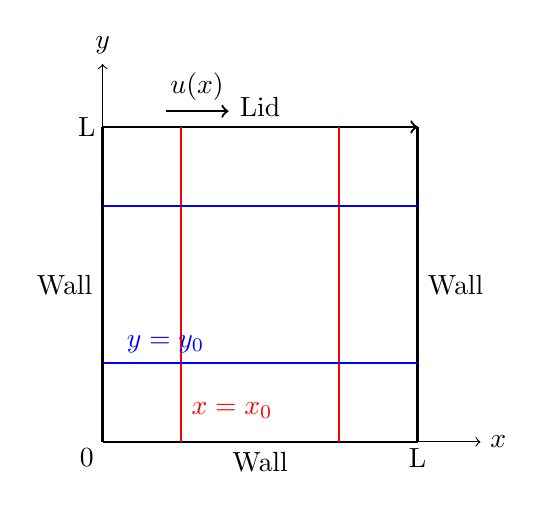
\begin{tikzpicture}[scale=4]
        % Eixos x e y
        \draw[->] (0,0) -- (1.2,0) node[right] {$x$};
        \draw[->] (0,0) -- (0,1.2) node[above] {$y$};
        % Desenhando o quadrado do domínio
        \draw (0,0) rectangle (1,1);
        % Desenho da tampa (lid)
        \draw[->, thick] (0,1) -- (1,1) node[midway, above] {Lid};
        \draw[-, thick]  (0,0) -- (1,0) node[midway, below] {Wall};
        \draw[-, thick]  (0,0) -- (0,1) node[midway, left] {Wall};
        \draw[-, thick]  (1,0) -- (1,1) node[midway, right] {Wall};
        \draw[->, thick] (0.2,1.05) -- (0.4,1.05) node[midway, above] {$u(x)$};
        % Outras anotações
        \node at (-0.05,-0.05) {0};
        \node at (1,-0.05) {L};
        \node at (-0.05,1) {L};
        % % Vortice central
        % \draw[thick] plot[smooth cycle] coordinates {(0.1,0.9) (0.9,0.9) (0.9,0.1) (0.1,0.1)};
        % \draw[thick] plot[smooth cycle] coordinates {(0.2,0.8) (0.8,0.8) (0.8,0.2) (0.2,0.2)};
        % \draw[thick] plot[smooth cycle] coordinates {(0.3,0.7) (0.7,0.7) (0.7,0.3) (0.3,0.3)};
        % \draw[thick] plot[smooth cycle] coordinates {(0.4,0.6) (0.6,0.6) (0.6,0.4) (0.4,0.4)};
        % \draw[->, thick] (0.62,0.5) -- (0.62,0.45);
        % \draw[->, thick] (0.741,0.5) -- (0.741,0.45);
        % \draw[->, thick] (0.8625,0.5) -- (0.8625,0.45);
        % \draw[->, thick] (0.982,0.5) -- (0.982,0.45);
        % % Vortice inferrior esquerdo
        % \draw[thick] plot[smooth cycle] coordinates {(0.07,0.05) (0.05,0.1) (0.1,0.05)};
        % \draw[thick] plot[smooth cycle] coordinates {(0.035,0.035) (0.04,0.13) (0.13,0.035)};
        % \draw[->, thick] (0.027,0.09) -- (0.027,0.042);
        % % Vortice inferior direito
        % \draw[thick] plot[smooth cycle] coordinates {(0.93,0.05) (0.95,0.091) (0.91,0.05)};
        % \draw[thick] plot[smooth cycle] coordinates {(0.97,0.035) (0.97,0.13) (0.87,0.035)};
        % \draw[->, thick] (0.976,0.05) -- (0.976,0.1);
        
        % Linha vertical em x = 0.5
        \draw[red, thick] (0.25, 0) -- (0.25, 1) node[pos=0.1, right] {$x = x_0$};
        \draw[red, thick] (0.75, 0) -- (0.75, 1) node[pos=0.1, right] {};
        % Linha horizontal em y = 0.5
        \draw[blue, thick] (0, 0.25) -- (1, 0.25) node[pos=0.2, above] {$y = y_0$};
        \draw[blue, thick] (0, 0.75) -- (1, 0.75) node[pos=0.2, above] {};
    \end{tikzpicture}
    }
    \caption{Schematic diagram of the computational domain used for the flow on a lid-driven cavity.\label{fig_domain}}
\end{figure}

\subsection{Manufactured Solution}

Firstly, we conducted a numerical study using a manufactured solution. To
ensure the accuracy of the code's order analysis, the manufactured solutions
must avoid polynomials of order less than or equal to four, due to the
high-order numerical methods employed in our study. Therefore, we propose
solutions based on trigonometric functions, such as sines and cosines, that
allow a rigorous verification of the accuracy order of the numerical methods
presented. Consequently, the proposed manufactured solutions are given by
\begin{gather}
    \begin{aligned}
        \overline{u}(x,y) &~= (x-1) x \sin(\pi x) \bigg(\sin(\pi y)+\pi y \cos(\pi y)\bigg) e^{-a t}.\label{eq:u_case0_2}
    \end{aligned}
\end{gather}
Using the procedure discussed in Section~\ref{sec_CodeVerification}, we obtain the following.
\begin{gather}
    \begin{aligned}
        \widetilde{v}(x,y) &~= -y\sin(\pi y)\bigg((2x-1)\sin(\pi x)+\pi(x-1)x\cos(\pi x)\bigg)e^{-a t},\label{eq:v_case0_2}
    \end{aligned}
\end{gather}
\begin{gather}
    \begin{aligned}
        \widetilde{\omega_{z}}(x,y) = 2\bigg(\pi(x-1)x\sin(\pi x)\cos(\pi y)+y\sin(\pi y) &~ \\ \left(\left(1-\pi^2(x-1)x\right)\sin(\pi x)+\pi(2x - 1)\cos(\pi x)\right)\bigg)e^{-a t},\label{eq:wz_case0_2}
    \end{aligned}
\end{gather}
\begin{gather}
    \begin{aligned}
        \widetilde{\Psi}(x,y) &~= (x-1) x y\sin(\pi x)\sin(\pi y) e^{-a t}.\label{eq:psi_case0_2}
    \end{aligned}
\end{gather}
Lastly, for the polymeric tensor components, we consider the following manufactured solutions:

\small
\begin{gather}
    \begin{aligned}
        \overline{T}_{xx}(x,y) &~= (1-\beta_{nn})\bigg(\sin(\pi x)+\cos(\pi x)+1\bigg)\bigg(\sin(\pi  y)+\cos (\pi y)+1\bigg)e^{-a t},\label{eq:txx_case0_2}
    \end{aligned}
\end{gather}
\begin{gather}
    \begin{aligned}
        \overline{T}_{xy}(x,y) &~= (1-\beta_{nn})\bigg(-\sin(\pi x)+\cos (\pi x)+1\bigg)\bigg(-\sin (\pi  y)+\cos (\pi  y)+1\bigg)e^{-a t},\label{eq:txy_case0_2}
    \end{aligned}
\end{gather}
\begin{gather}
    \begin{aligned}
        \overline{T}_{yy}(x,y) &~= (1-\beta_{nn})\bigg(\sin(\pi x)-\cos(\pi  x)+1\bigg)\bigg(\sin(\pi y)-\cos(\pi y)+1\bigg)e^{-a t}.\label{eq:tyy_case0_2}
    \end{aligned}
\end{gather}

\normalsize

For an accurate comparison of the numerical results obtained by the code under
evaluation, we introduced a multiplicative factor of $(1-\beta_{nn})$ in the
manufactured solution of the polymeric tensor components. It is important to
note that in scenarios involving Newtonian flows, where $\beta_{nn} = 1$, this
multiplicative factor effectively cancels the contribution of the polymeric
tensor components. As a result, the solution aligns with the behaviour of a
Newtonian fluid flow. Figures~\ref{U_m_u_sol_num_case1map2} and
\ref{T_m_u_sol_num_case1map2} illustrate manufactured solutions in the
steady-state regime, using $a = 0.05$ and $\beta_{nn}=0.1$.

\begin{figure}[H]
    \centering
    \begin{subfigure}[b]{.46\textwidth}
        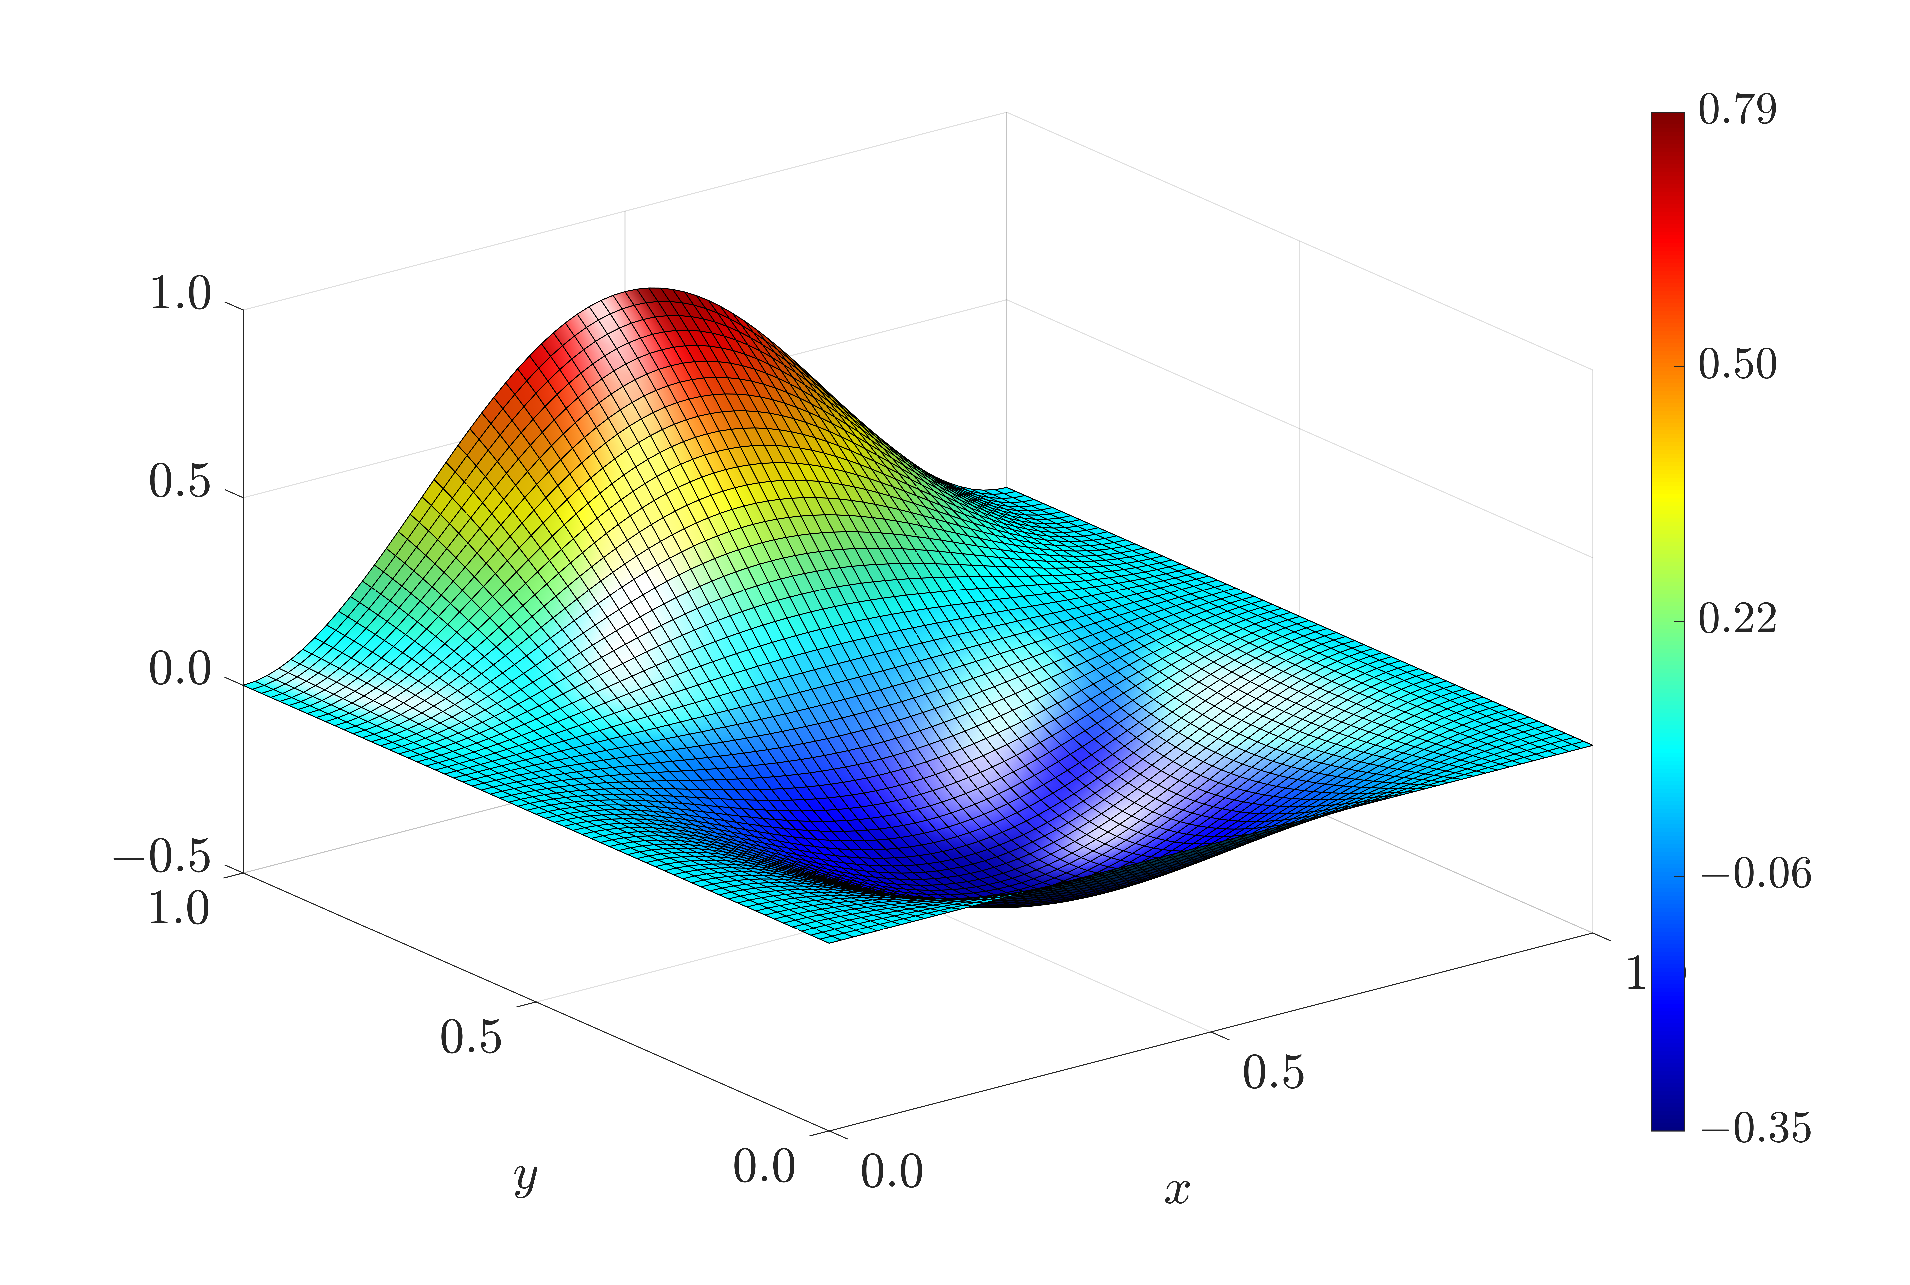
\includegraphics[width=\textwidth]{Exact_Surf_NormErr_2nd_Betann_0.1_Re_1_Wi_1_epsilon_0_xi_0_alphaG_0_Dt_1e-06_at_0.05_tipsim_1_MMS_12_U.eps}
        \caption{$\overline{u}$\label{fig:solexauCase1}}
    \end{subfigure}
    \vspace{0.2cm}
    \begin{subfigure}[b]{.46\textwidth}
        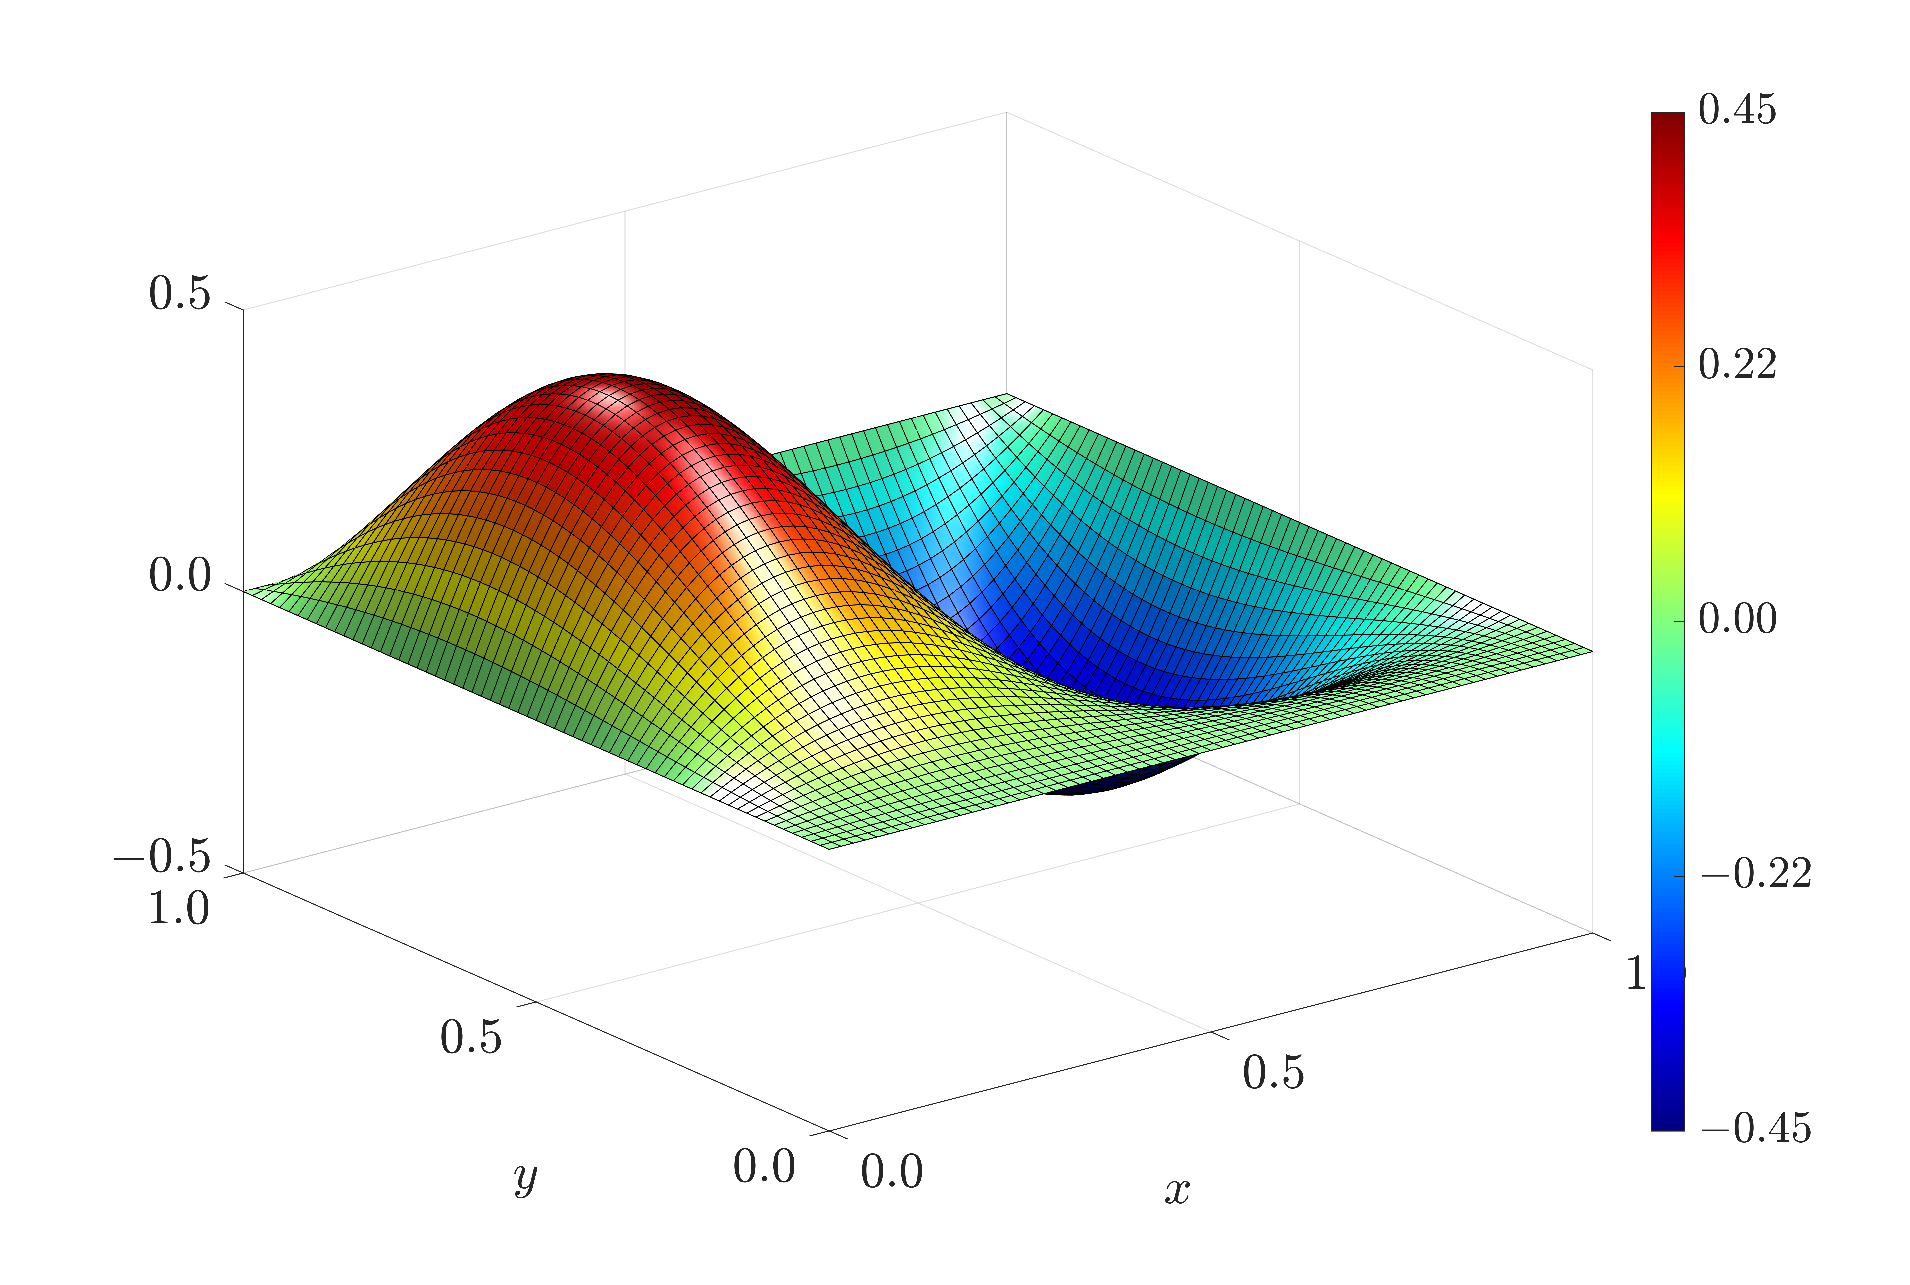
\includegraphics[width=\textwidth]{Exact_Surf_NormErr_2nd_Betann_0.1_Re_1_Wi_1_epsilon_0_xi_0_alphaG_0_Dt_1e-06_at_0.05_tipsim_1_MMS_12_V.eps}
        \caption{$\widetilde{v}$\label{fig:solexavCase1}}
    \end{subfigure}
    \begin{subfigure}[b]{.46\textwidth}
        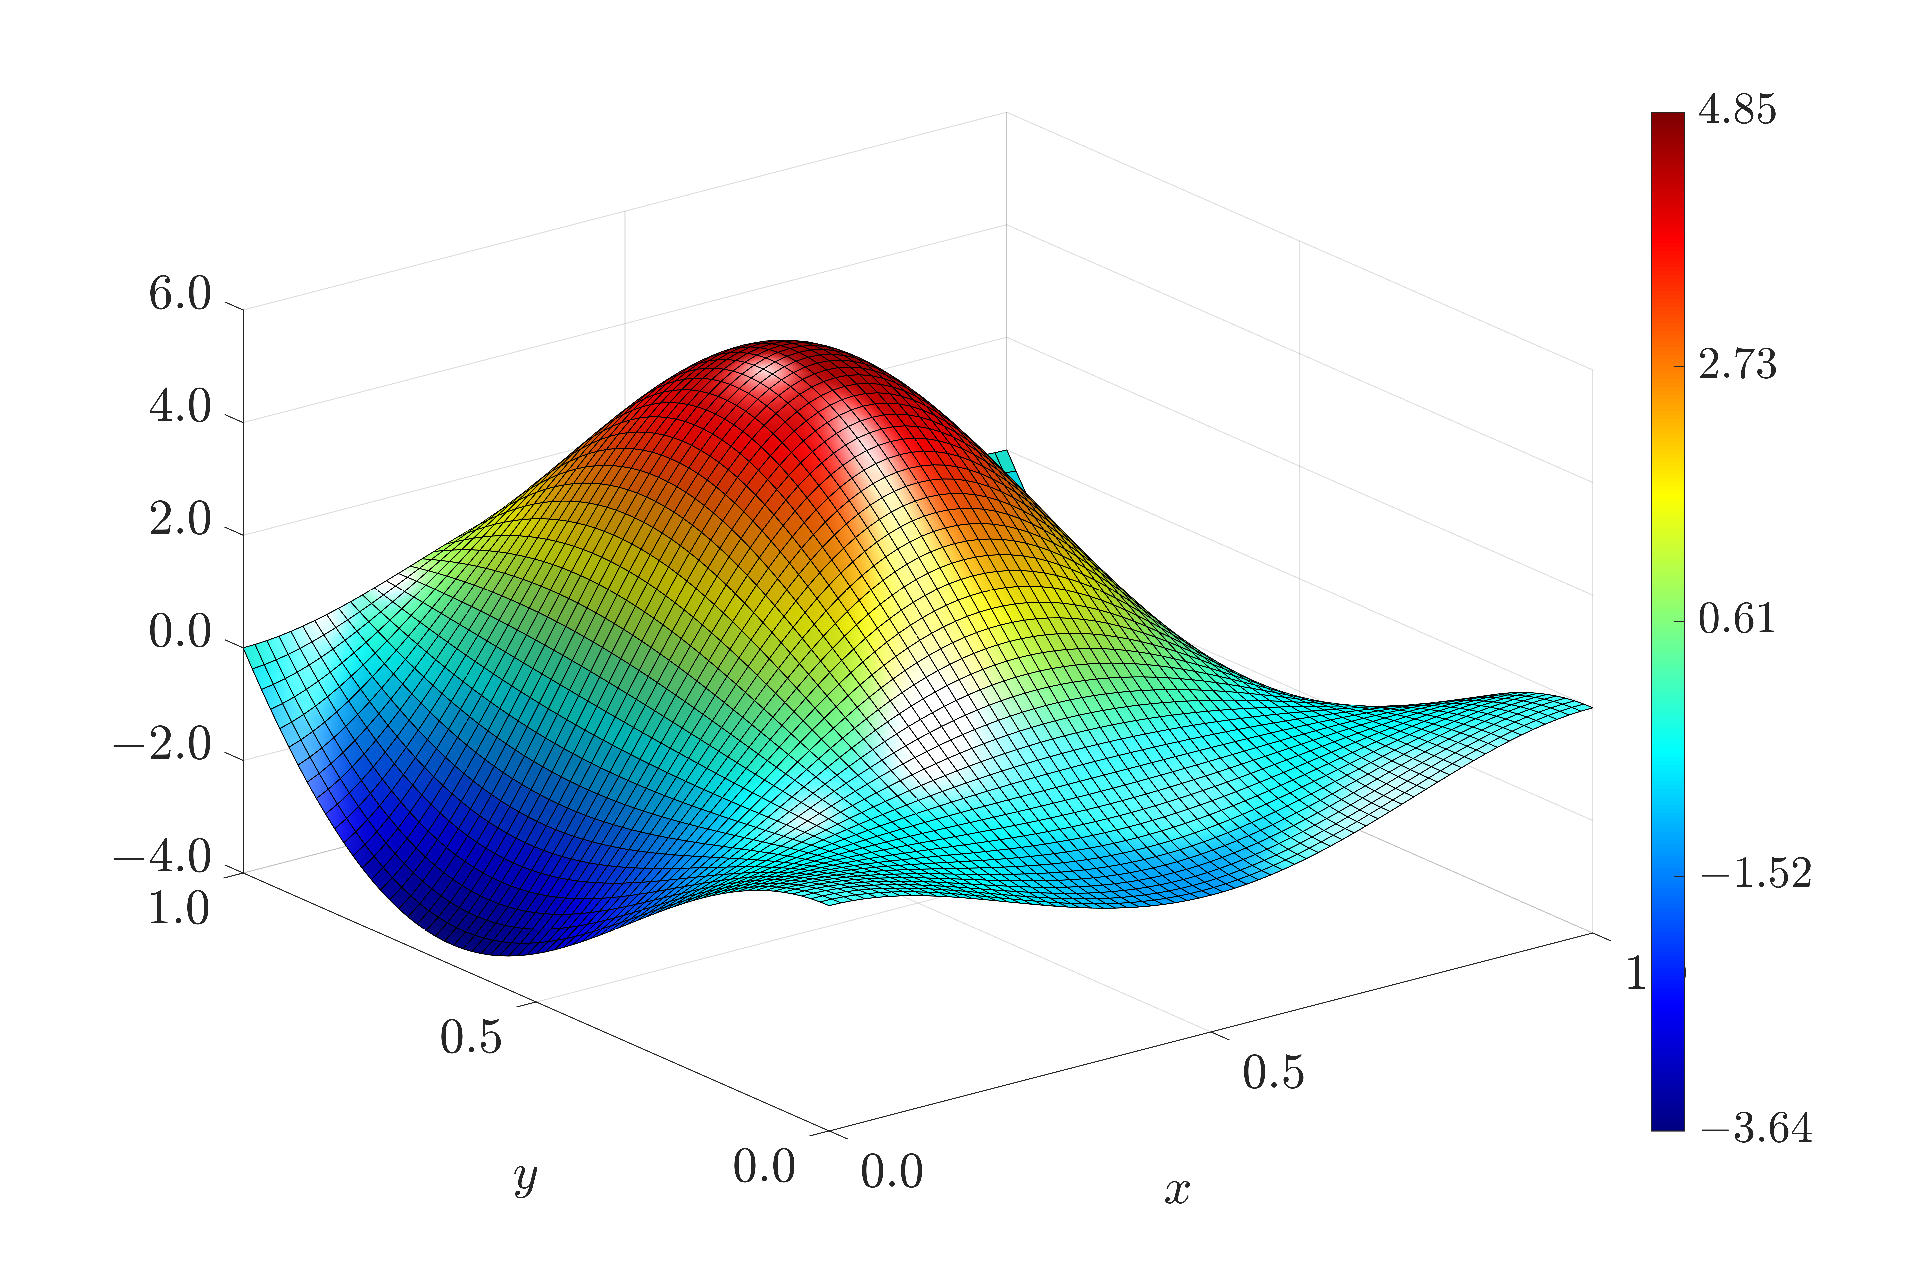
\includegraphics[width=\textwidth]{Exact_Surf_NormErr_2nd_Betann_0.1_Re_1_Wi_1_epsilon_0_xi_0_alphaG_0_Dt_1e-06_at_0.05_tipsim_1_MMS_12_Wz.eps}
        \caption{$\widetilde{\omega}_{z}$\label{fig:solexawzCase1}}
    \end{subfigure}
    \vspace{0.2cm}
    \begin{subfigure}[b]{.46\textwidth}
        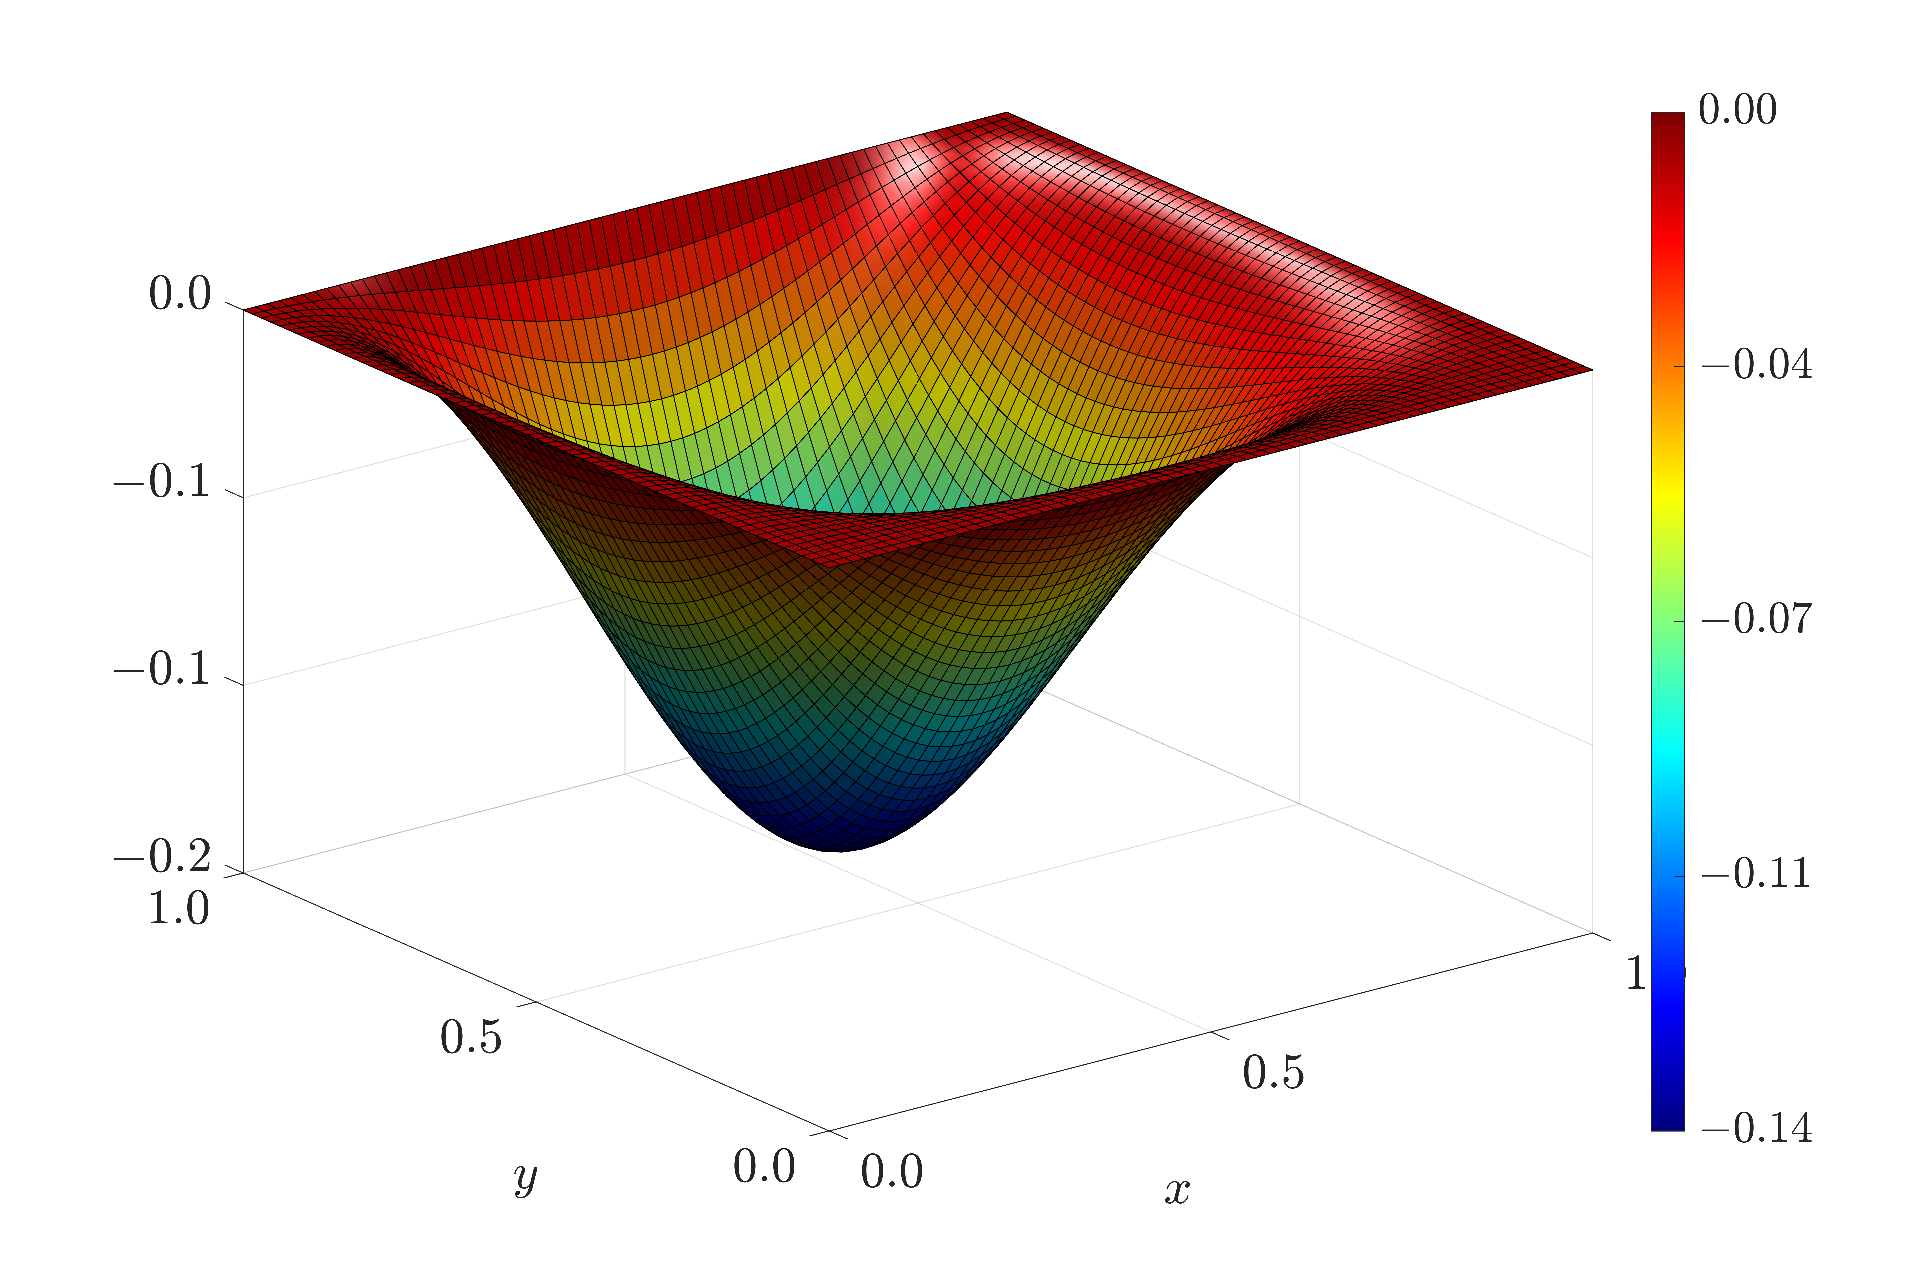
\includegraphics[width=\textwidth]{Exact_Surf_NormErr_2nd_Betann_0.1_Re_1_Wi_1_epsilon_0_xi_0_alphaG_0_Dt_1e-06_at_0.05_tipsim_1_MMS_12_Psi.eps}
        \caption{$\widetilde{\Psi}$\label{fig:solexapsiCase1}}
    \end{subfigure}
    \vspace{0.02cm}
    \caption{Manufactured solutions in the steady-state regime for the velocity field $(\overline{u},\widetilde{v})$, vorticity $(\widetilde{\omega}_{z})$, and stream function $(\widetilde{\Psi})$, using $\beta_{nn}=0.1$ and $a = 0.05$.\label{U_m_u_sol_num_case1map2}}
\end{figure}

\begin{figure}
    \begin{subfigure}[b]{.46\textwidth}
        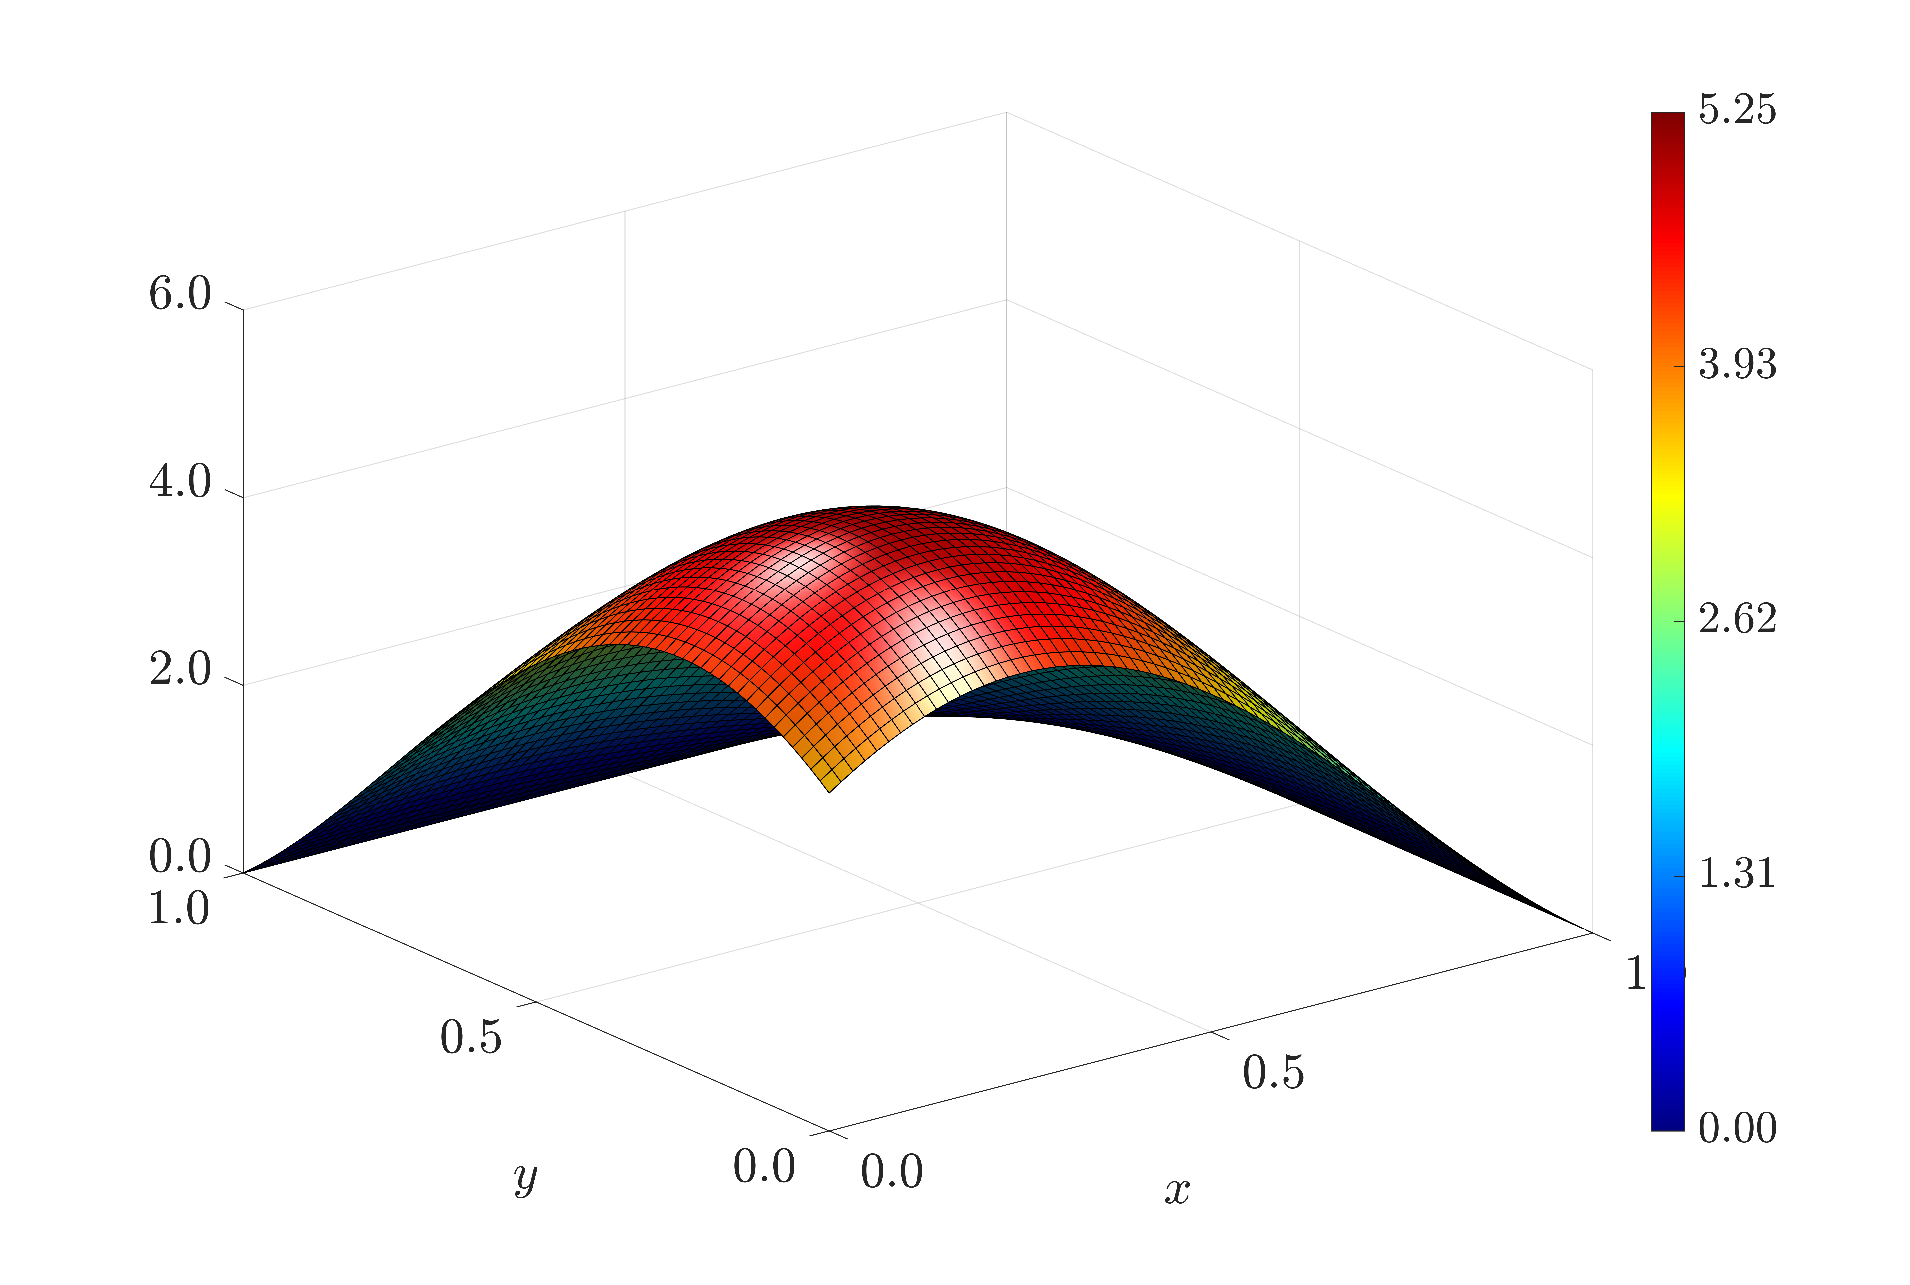
\includegraphics[width=\textwidth]{Exact_Surf_NormErr_2nd_Betann_0.1_Re_1_Wi_1_epsilon_0_xi_0_alphaG_0_Dt_1e-06_at_0.05_tipsim_1_MMS_12_Txx.eps}
        \caption{$\overline{T}_{xx}$}
        \label{fig:solexaTxxCase1}
    \end{subfigure}
    \vspace{0.2cm}
    \begin{subfigure}[b]{.46\textwidth}
        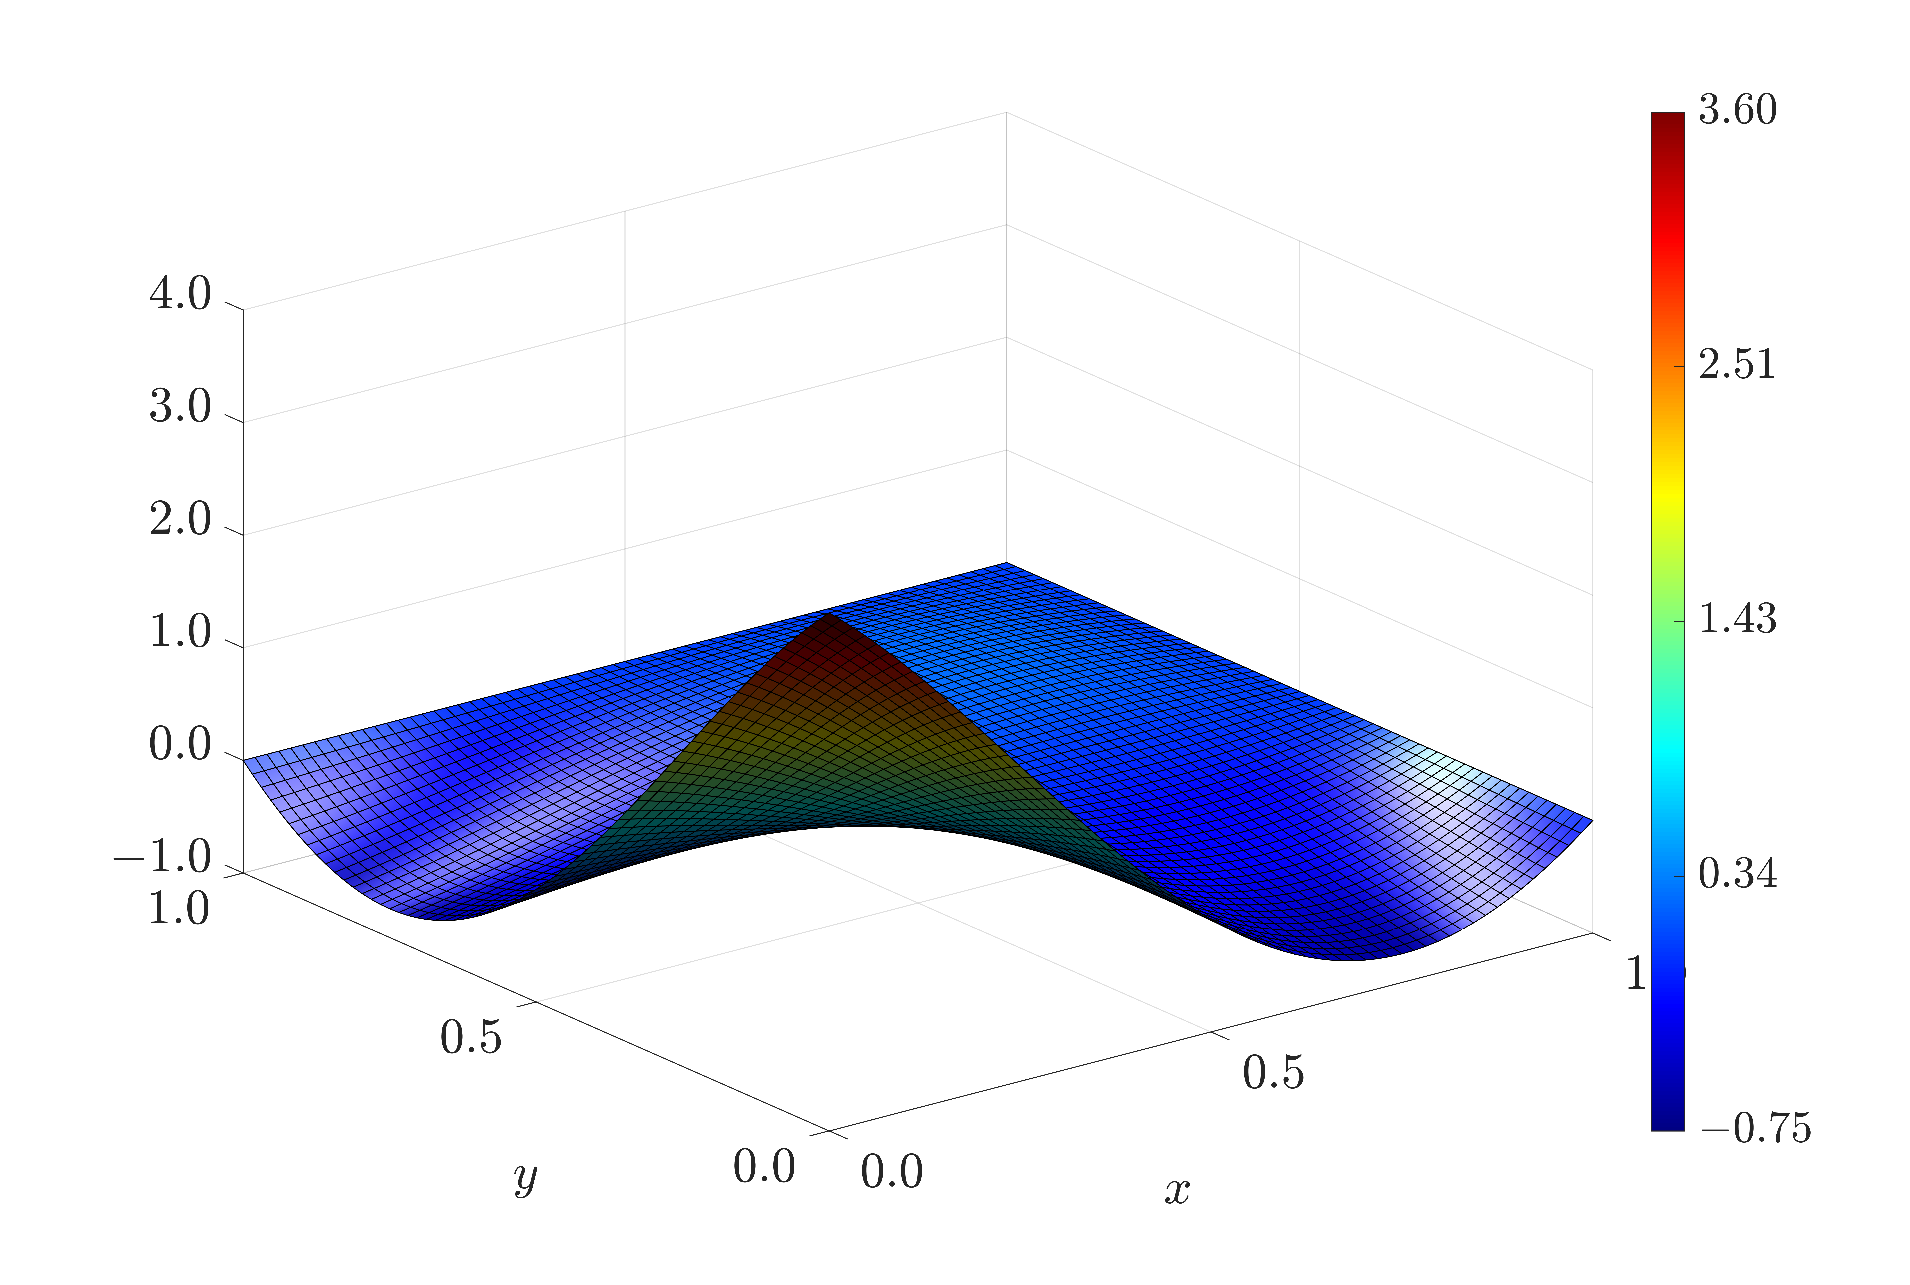
\includegraphics[width=\textwidth]{Exact_Surf_NormErr_2nd_Betann_0.1_Re_1_Wi_1_epsilon_0_xi_0_alphaG_0_Dt_1e-06_at_0.05_tipsim_1_MMS_12_Txy.eps}
        \caption{$\overline{T}_{xy}$}
        \label{fig:solexaTxyCase1}
    \end{subfigure}
    \begin{subfigure}[b]{.46\textwidth}
        \includegraphics[width=\textwidth]{Exact_Surf_NormErr_2nd_Betann_0.1_Re_1_Wi_1_epsilon_0_xi_0_alphaG_0_Dt_1e-06_at_0.05_tipsim_1_MMS_12_Tyy.eps}
        \caption{$\overline{T}_{yy}$}
        \label{fig:solexaTyyCase1}
    \end{subfigure}
    \vspace{0.02cm}
    \caption{Manufactured solutions in the steady-state regime for the polymeric tensor components, using $\beta_{nn}=0.1$ and $a = 0.05$.\label{T_m_u_sol_num_case1map2}}
\end{figure}

Figures~\ref{fig_U_m_u_sol_num_case1streamline2} and
\ref{fig_Txxxyyy_m_u_sol_num_case1streamline2} illustrate the contours of the
manufactured solutions in the steady-state regime, using $\beta_{nn}=0.1$ and
$a = 0.05$. In addition, Figures~\ref{fig_U_m_u_sol_num_case1streamline2} and
\ref{fig_Txxxyyy_m_u_sol_num_case1streamline2} show the contour map of the
manufactured solutions in the steady-state regime. Figures show that the
proposed manufactured solutions follow the flow pattern of the lid-driven
cavity problem, as presented in \citet{bruneau20062d}. The fact that the
manufactured solutions are composed of trigonometric functions allows them to
be used for testing higher-order numerical schemes due to the simple fact that
these functions are infinitely differentiable and their derivatives are not
identically zero. These features provide a robust framework for evaluating the
accuracy and convergence of numerical schemes designed to solve complex
viscoelastic fluid flow problems.
\begin{figure}[H]
    \centering
    \begin{subfigure}[b]{.46\textwidth}
        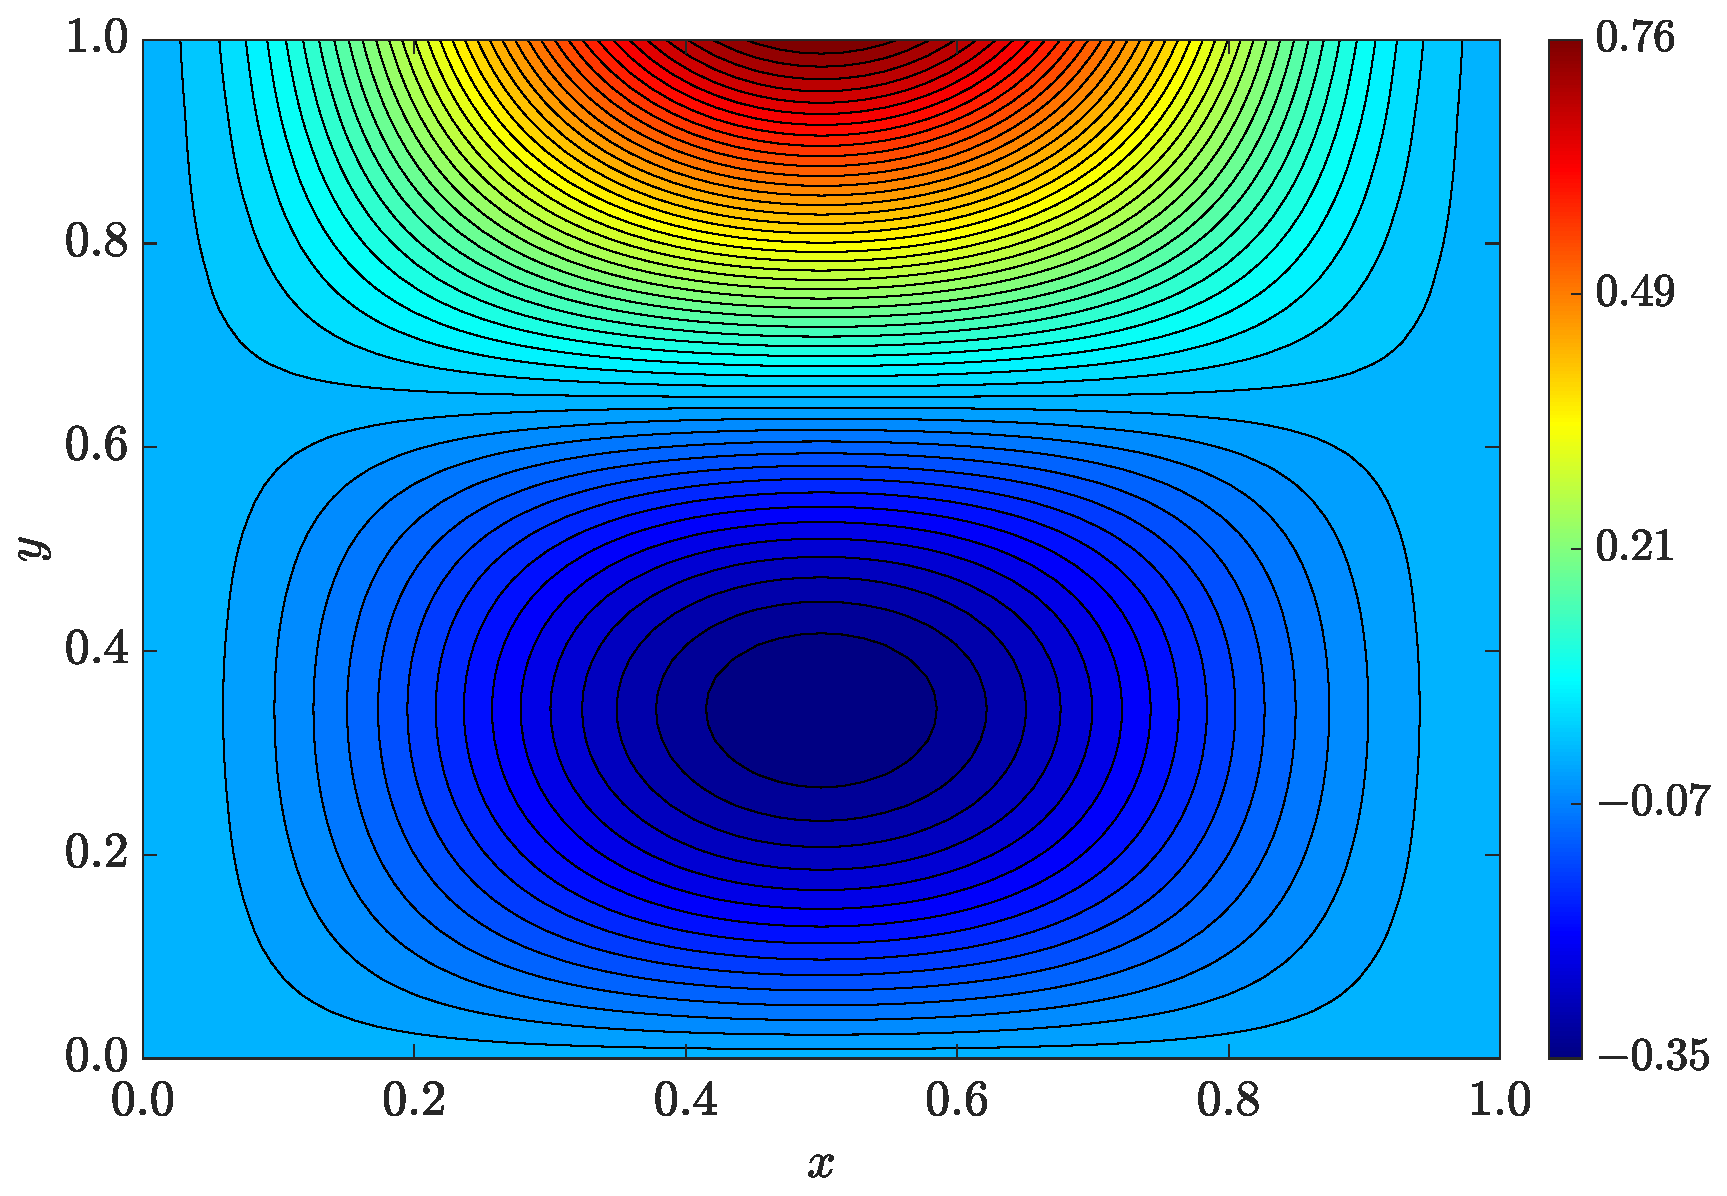
\includegraphics[width=\textwidth]{Exact_Map_NormErr_2nd_Betann_0.1_Re_1_Wi_1_epsilon_0_xi_0_alphaG_0_Dt_1e-06_at_0.05_tipsim_1_MMS_12_U.eps}
        \caption{$\overline{u}$}
        \label{fig_solexaustreamlineCase1}
    \end{subfigure}
    \vspace{0.2cm}
    \begin{subfigure}[b]{.46\textwidth}
        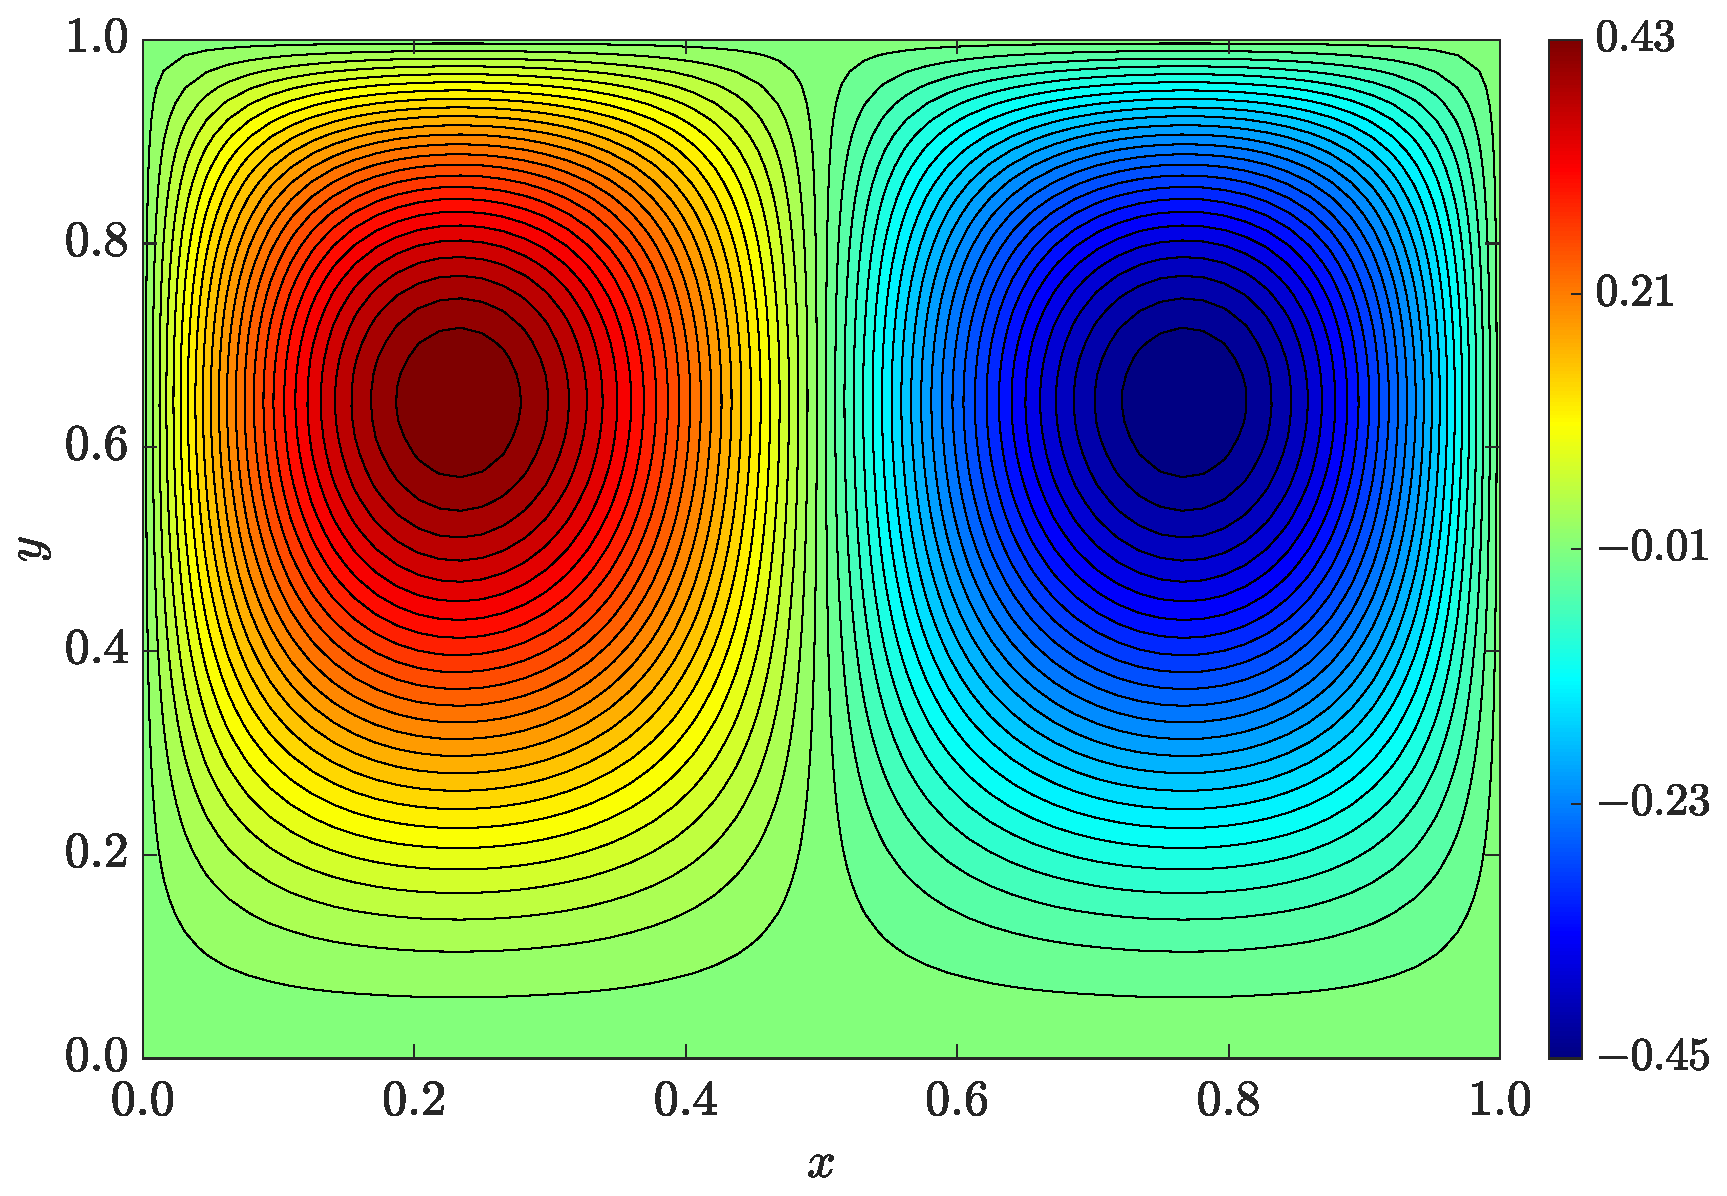
\includegraphics[width=\textwidth]{Exact_Map_NormErr_2nd_Betann_0.1_Re_1_Wi_1_epsilon_0_xi_0_alphaG_0_Dt_1e-06_at_0.05_tipsim_1_MMS_12_V.eps}
        \caption{$\widetilde{v}$}
        \label{fig_solexavstreamlineCase1}
    \end{subfigure}
    \begin{subfigure}[b]{.46\textwidth}
        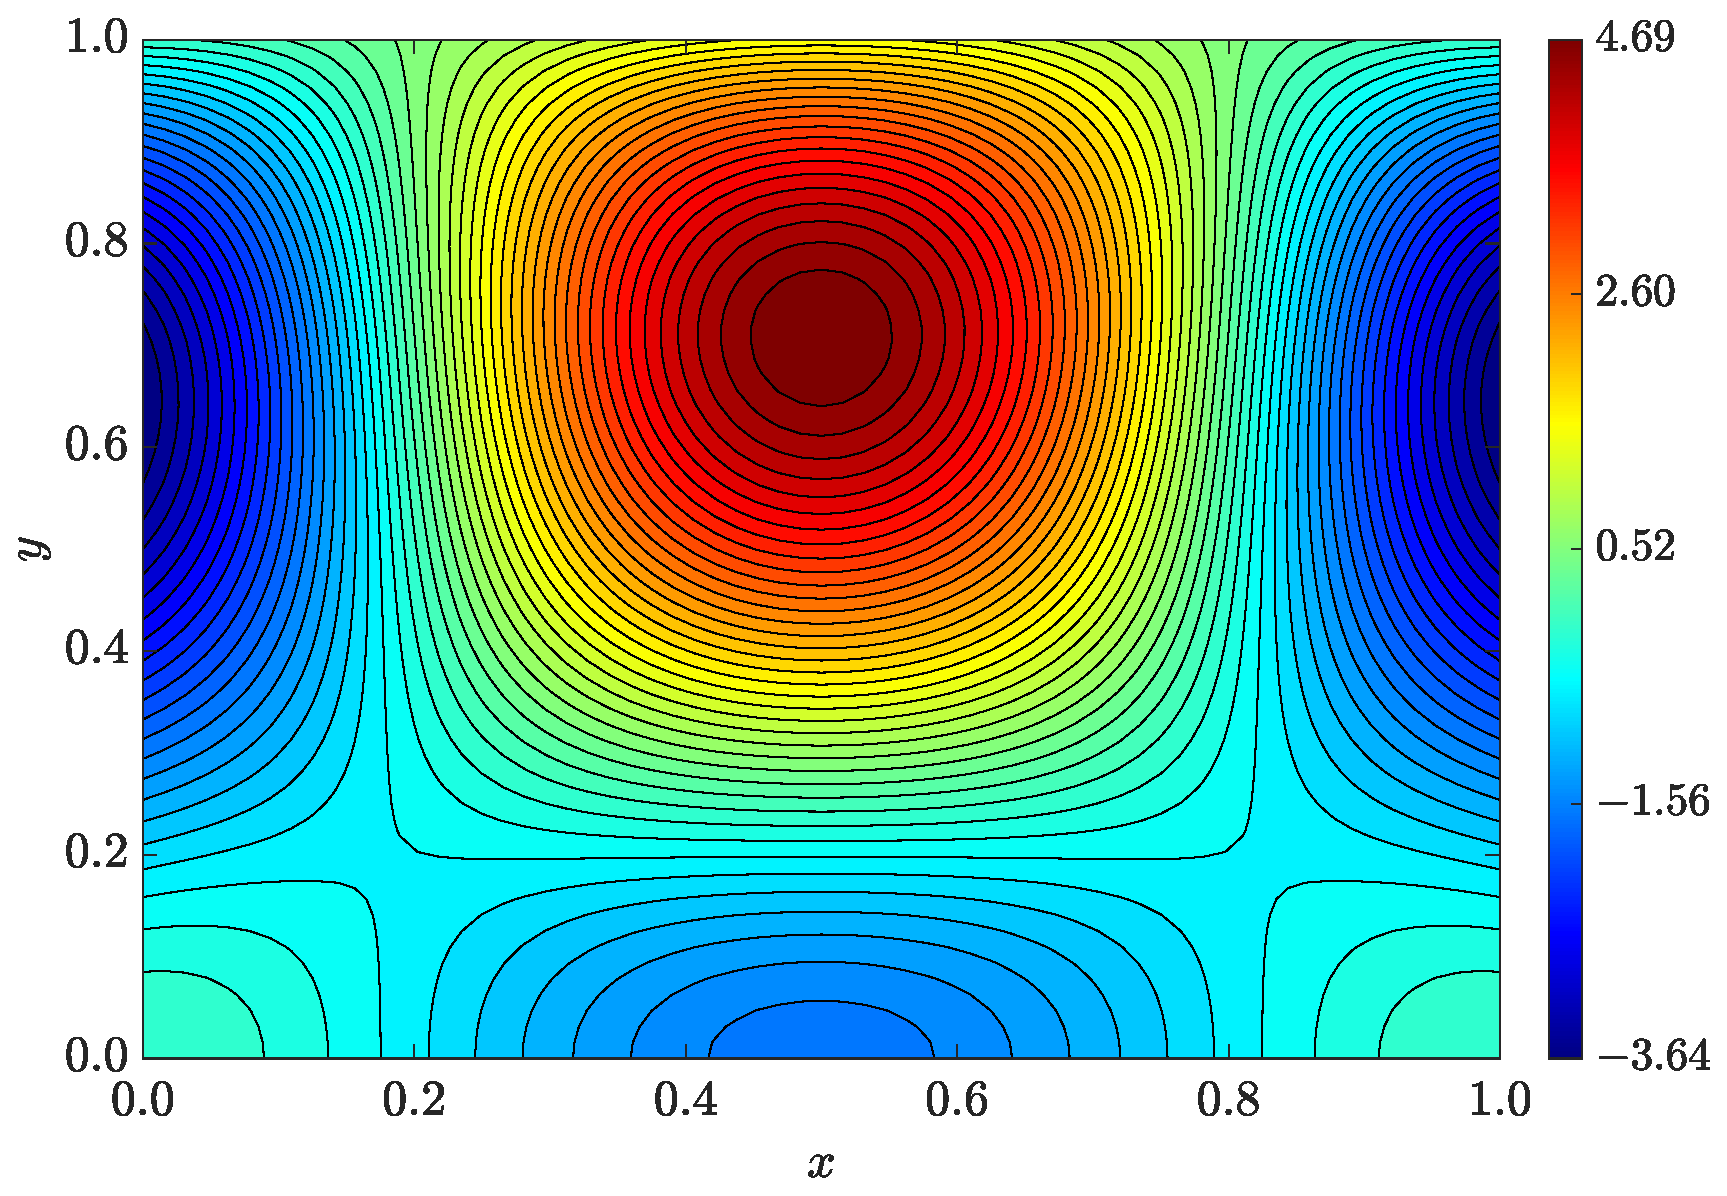
\includegraphics[width=\textwidth]{Exact_Map_NormErr_2nd_Betann_0.1_Re_1_Wi_1_epsilon_0_xi_0_alphaG_0_Dt_1e-06_at_0.05_tipsim_1_MMS_12_Wz.eps}
        \caption{$\widetilde{\omega_{z}}$}
        \label{fig_solexawzstreamlineCase1}
    \end{subfigure}
    \vspace{0.2cm}
    \begin{subfigure}[b]{.46\textwidth}
        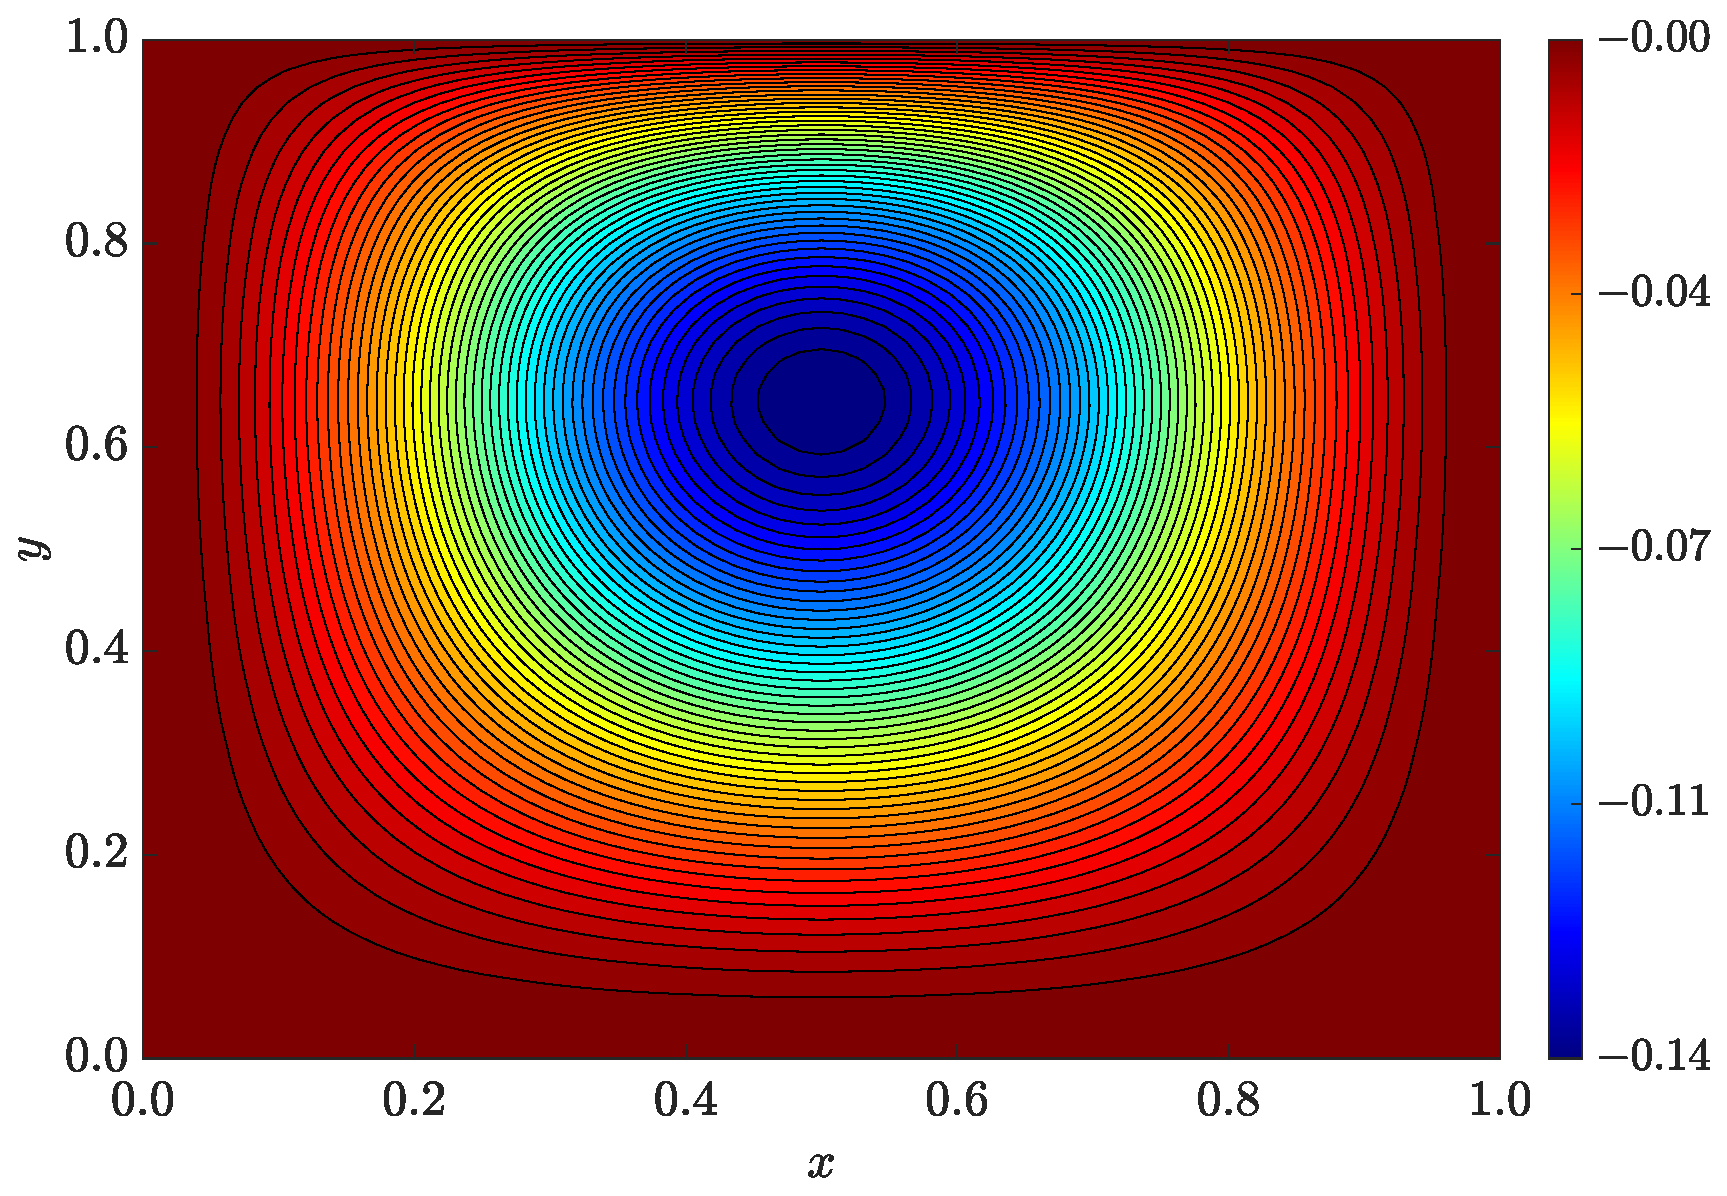
\includegraphics[width=\textwidth]{Exact_Map_NormErr_2nd_Betann_0.1_Re_1_Wi_1_epsilon_0_xi_0_alphaG_0_Dt_1e-06_at_0.05_tipsim_1_MMS_12_Psi.eps}
        \caption{$\widetilde{\Psi}$}
        \label{fig_solexapsistreamlineCase1}
    \end{subfigure}
    \vspace{0.02cm}
    \caption{Contours of the manufactured solutions in the steady-state regime for the velocity field $(\overline{u},\widetilde{v})$, vorticity $(\widetilde{\omega_{z}})$, and stream function $(\widetilde{\Psi})$, using $\beta_{nn}=0.1$ and $a = 0.05$.\label{fig_U_m_u_sol_num_case1streamline2}}
\end{figure}
\begin{figure}[H]
    \centering
    \begin{subfigure}[b]{.46\textwidth}
        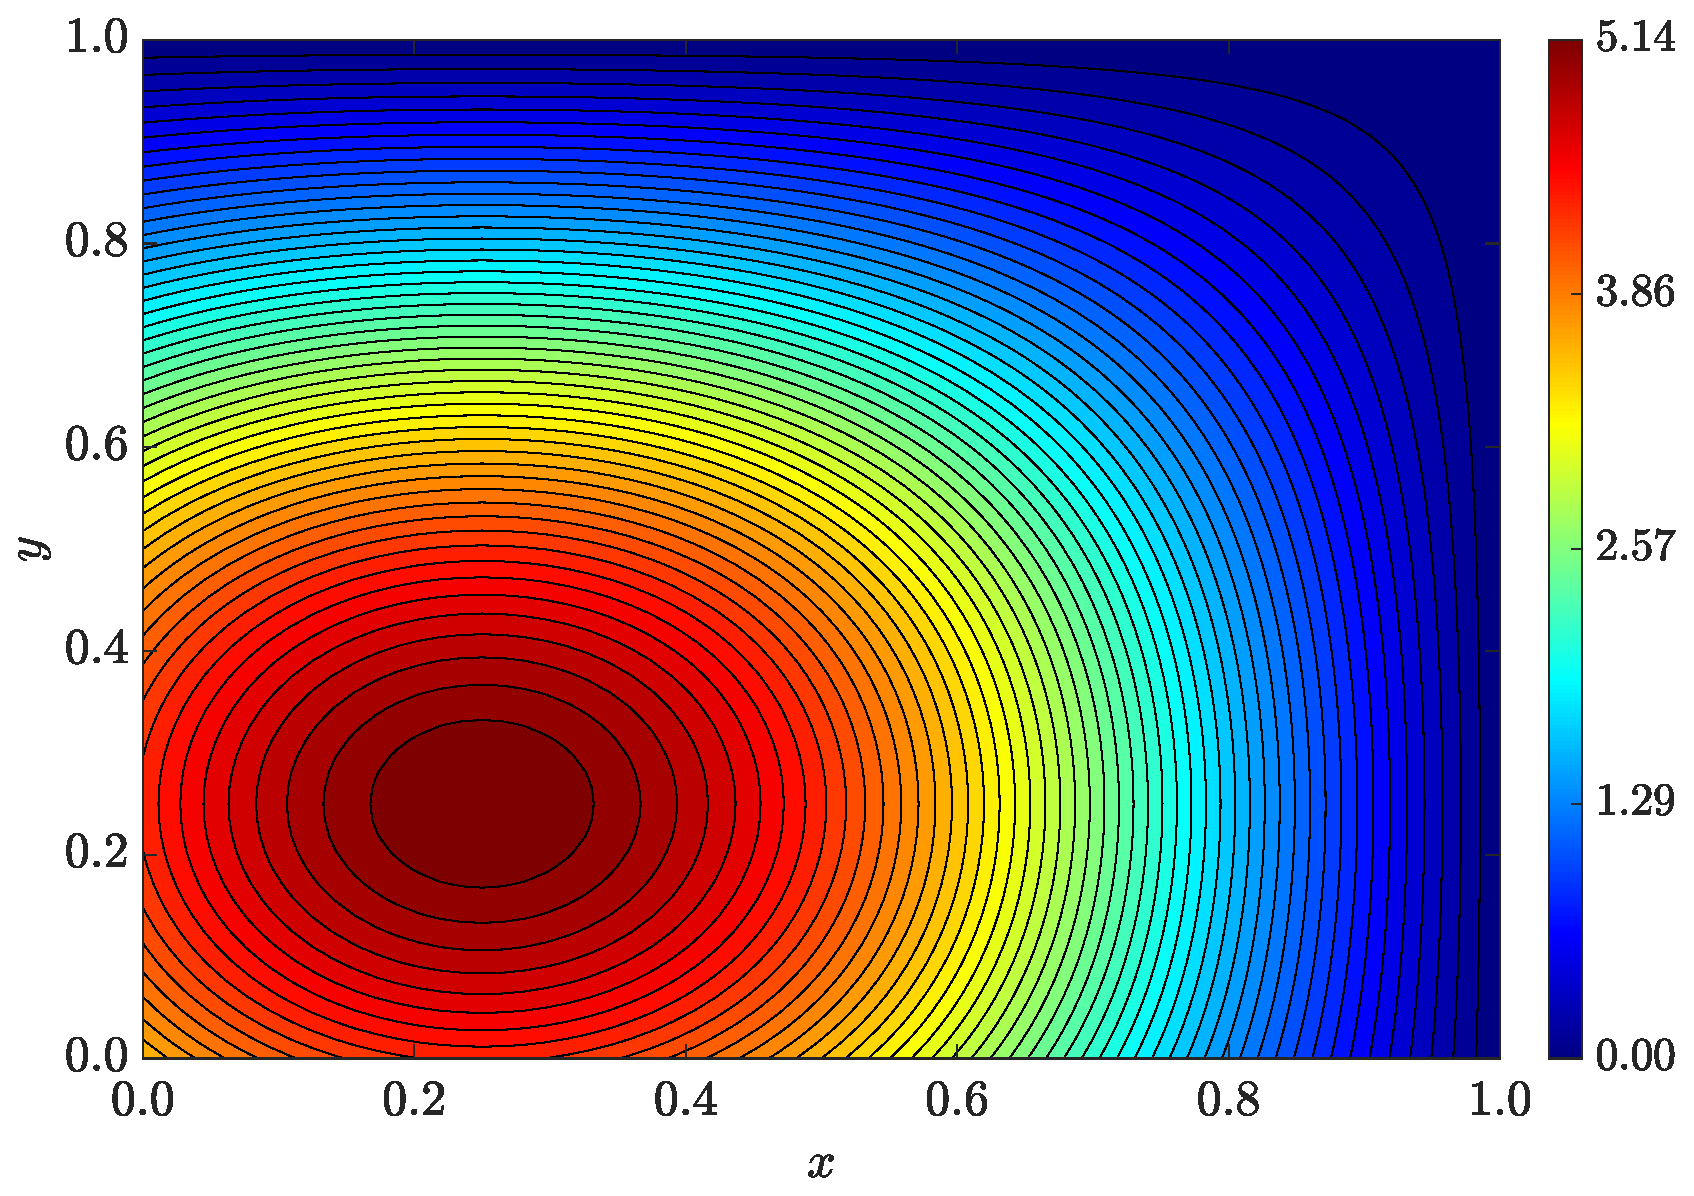
\includegraphics[width=\textwidth]{Exact_Map_NormErr_2nd_Betann_0.1_Re_1_Wi_1_epsilon_0_xi_0_alphaG_0_Dt_1e-06_at_0.05_tipsim_1_MMS_12_Txx.eps}
        \caption{$\overline{T}_{xx}$}
        \label{fig_solexatxxstreamlineCase1}
    \end{subfigure}
    \vspace{0.2cm}
    \begin{subfigure}[b]{.46\textwidth}
        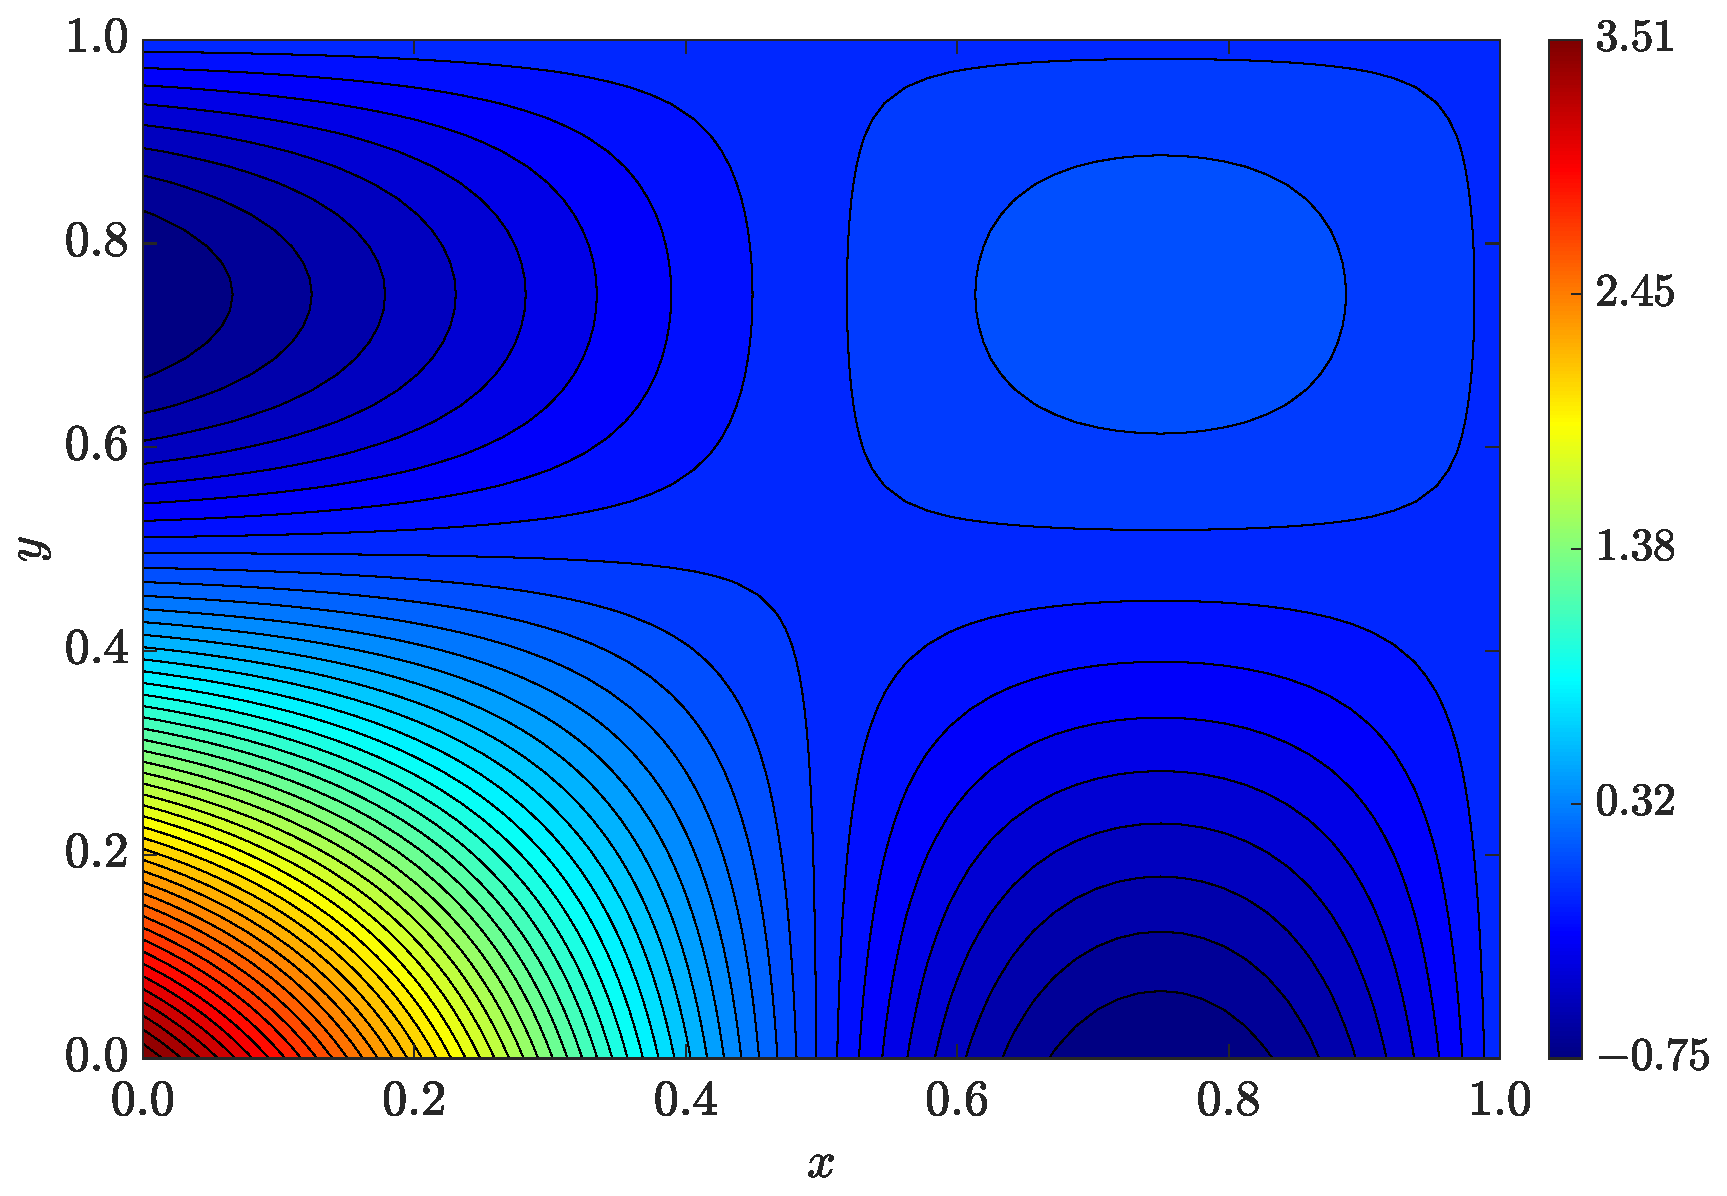
\includegraphics[width=\textwidth]{Exact_Map_NormErr_2nd_Betann_0.1_Re_1_Wi_1_epsilon_0_xi_0_alphaG_0_Dt_1e-06_at_0.05_tipsim_1_MMS_12_Txy.eps}
        \caption{$\overline{T}_{xy}$}
        \label{fig_solexatxystreamlineCase1}
    \end{subfigure}
    \begin{subfigure}[b]{.46\textwidth}
        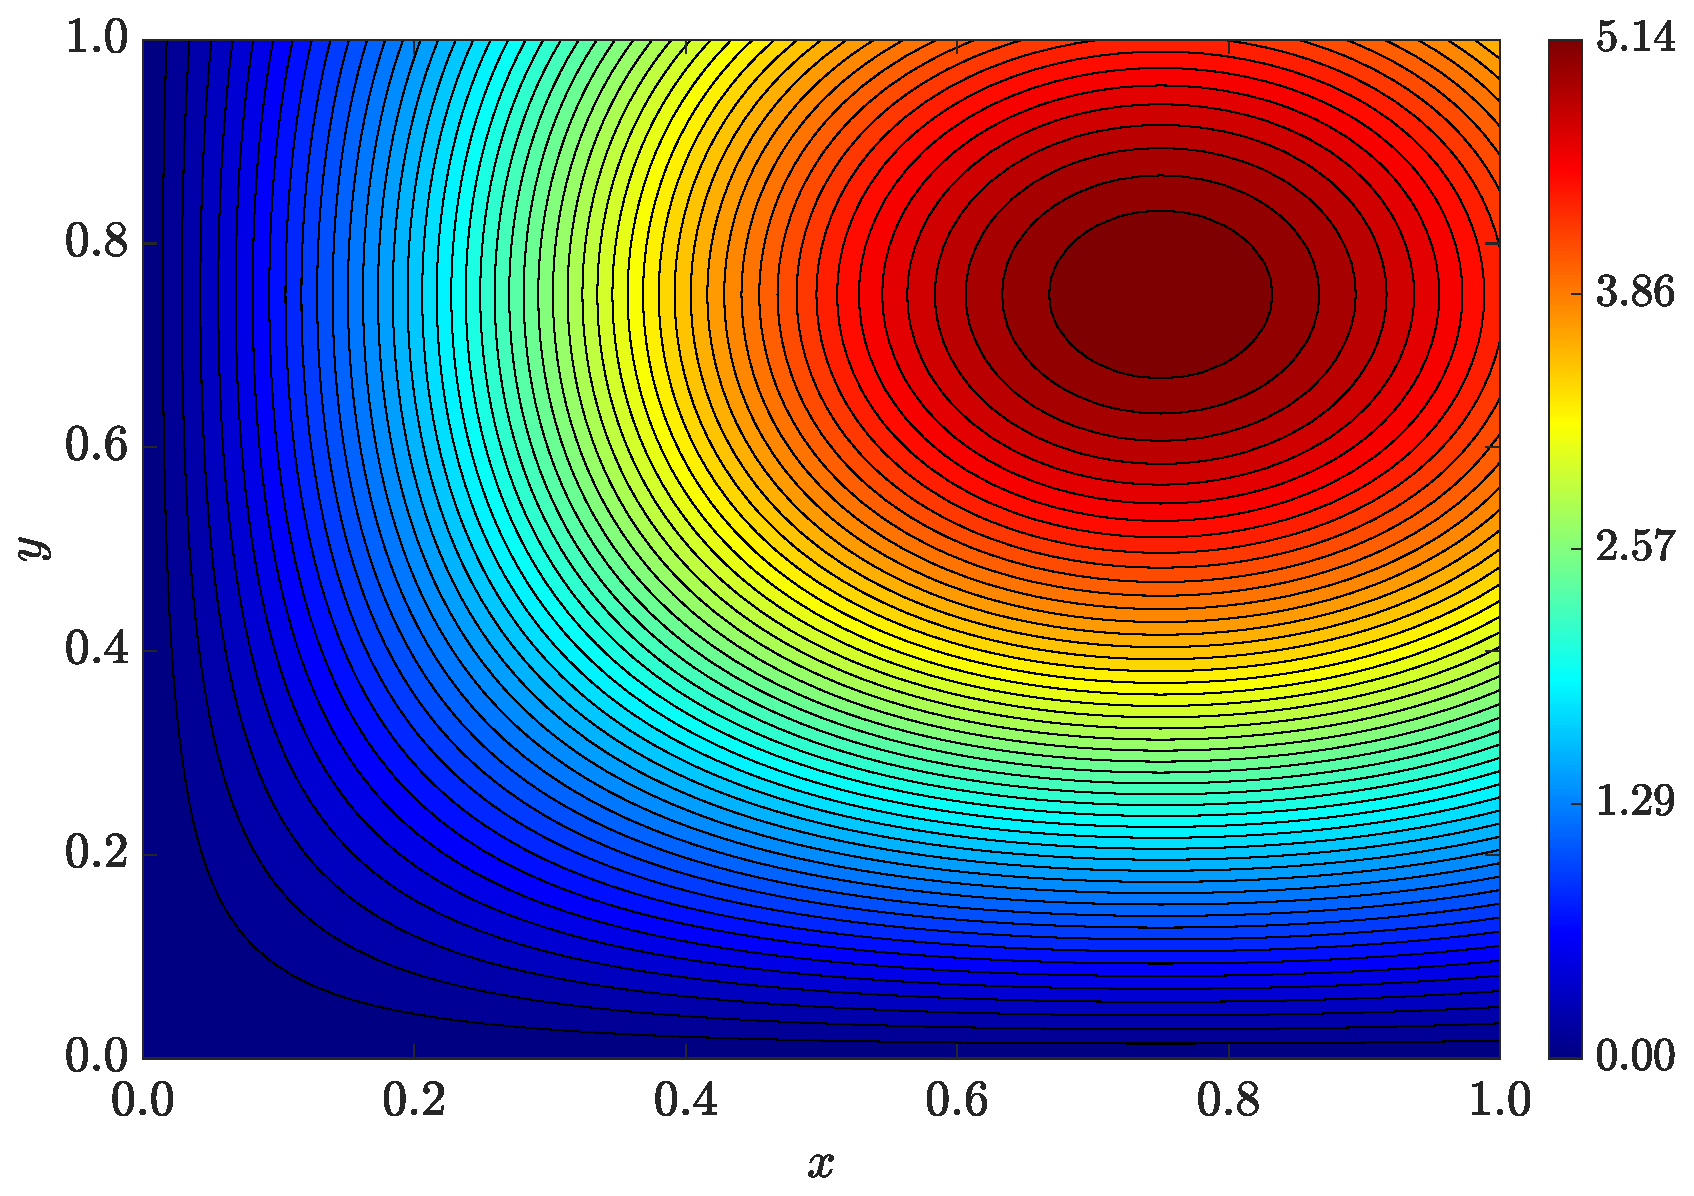
\includegraphics[width=\textwidth]{Exact_Map_NormErr_2nd_Betann_0.1_Re_1_Wi_1_epsilon_0_xi_0_alphaG_0_Dt_1e-06_at_0.05_tipsim_1_MMS_12_Tyy.eps}
        \caption{$\overline{T}_{yy}$}
        \label{fig_solexatyystreamlineCase1}
    \end{subfigure}
    \vspace{0.02cm}
    \caption{Contours of the manufactured solutions in the steady-state regime for the polymeric tensor components, using $\beta_{nn}=0.1$ and $a = 0.05$.\label{fig_Txxxyyy_m_u_sol_num_case1streamline2}}
\end{figure}

\subsection{Verification case using the Oldroyd-B constitutive model}
\label{subsec_oldroydb}

The numerical simulations conducted to verify the newly developed high-order
code for the calculation of viscoelastic fluid flows were set up using the
Oldroyd-B constitutive model with Reynolds number equal to
$\operatorname{Re}=1,\ 10,\ 100,\ 400,$ and $1000$, and a fixed Weissenberg
number of $Wi=1$. In addition, the solvent viscosity ratio was set equal to
$\beta_{nn} = 0.1,\ 0.5,\ 0.9,$ and $1.0$ to evaluate the performance of the
constitutive model under different flow regimes. The value of $\beta_{nn} =
1.0$ corresponds to Newtonian fluid behaviour, while lower values represent
increasingly viscoelastic fluid behaviour. It is important to note that the
Oldroyd-B constitutive model is obtained from Equation~(\ref{eq_geral_tensors})
by setting the parameter $\alpha_{G} = 0$, which simplifies the constitutive
model to the classical viscoelastic case without stress anisotropy.

Figure~\ref{fig_OldroydB_error_uvwzpsi} presents the error versus grid sizes
($\Delta x, \Delta y$) for the velocity field components, vorticity, and stream
function, while Figure~\ref{fig_OldroydB_error_txxxyyy} complements this
analysis by showing the errors associated with the polymeric tensor components
for the flow of an Oldroyd-B viscoelastic fluid. These plots illustrate the
evolution of errors for $\operatorname{Re}=100$, $Wi=1$, and $\beta_{nn}=0.1,\
0.5,\ 0.9$. It is important to note that the results for $\beta_{nn}=1.0$ have
been omitted, since the corresponding errors were of the order $10^{-18}$,
which would have distorted the comparative visualization of the other values of
$\beta_{nn}$. Lastly, Table~\ref{tab_OldroydBWzResumida} summarizes the
convergence order and the errors computed across the meshes considered.
\begin{figure}[H]
    \centering  
    \begin{subfigure}[b]{.46\textwidth}
        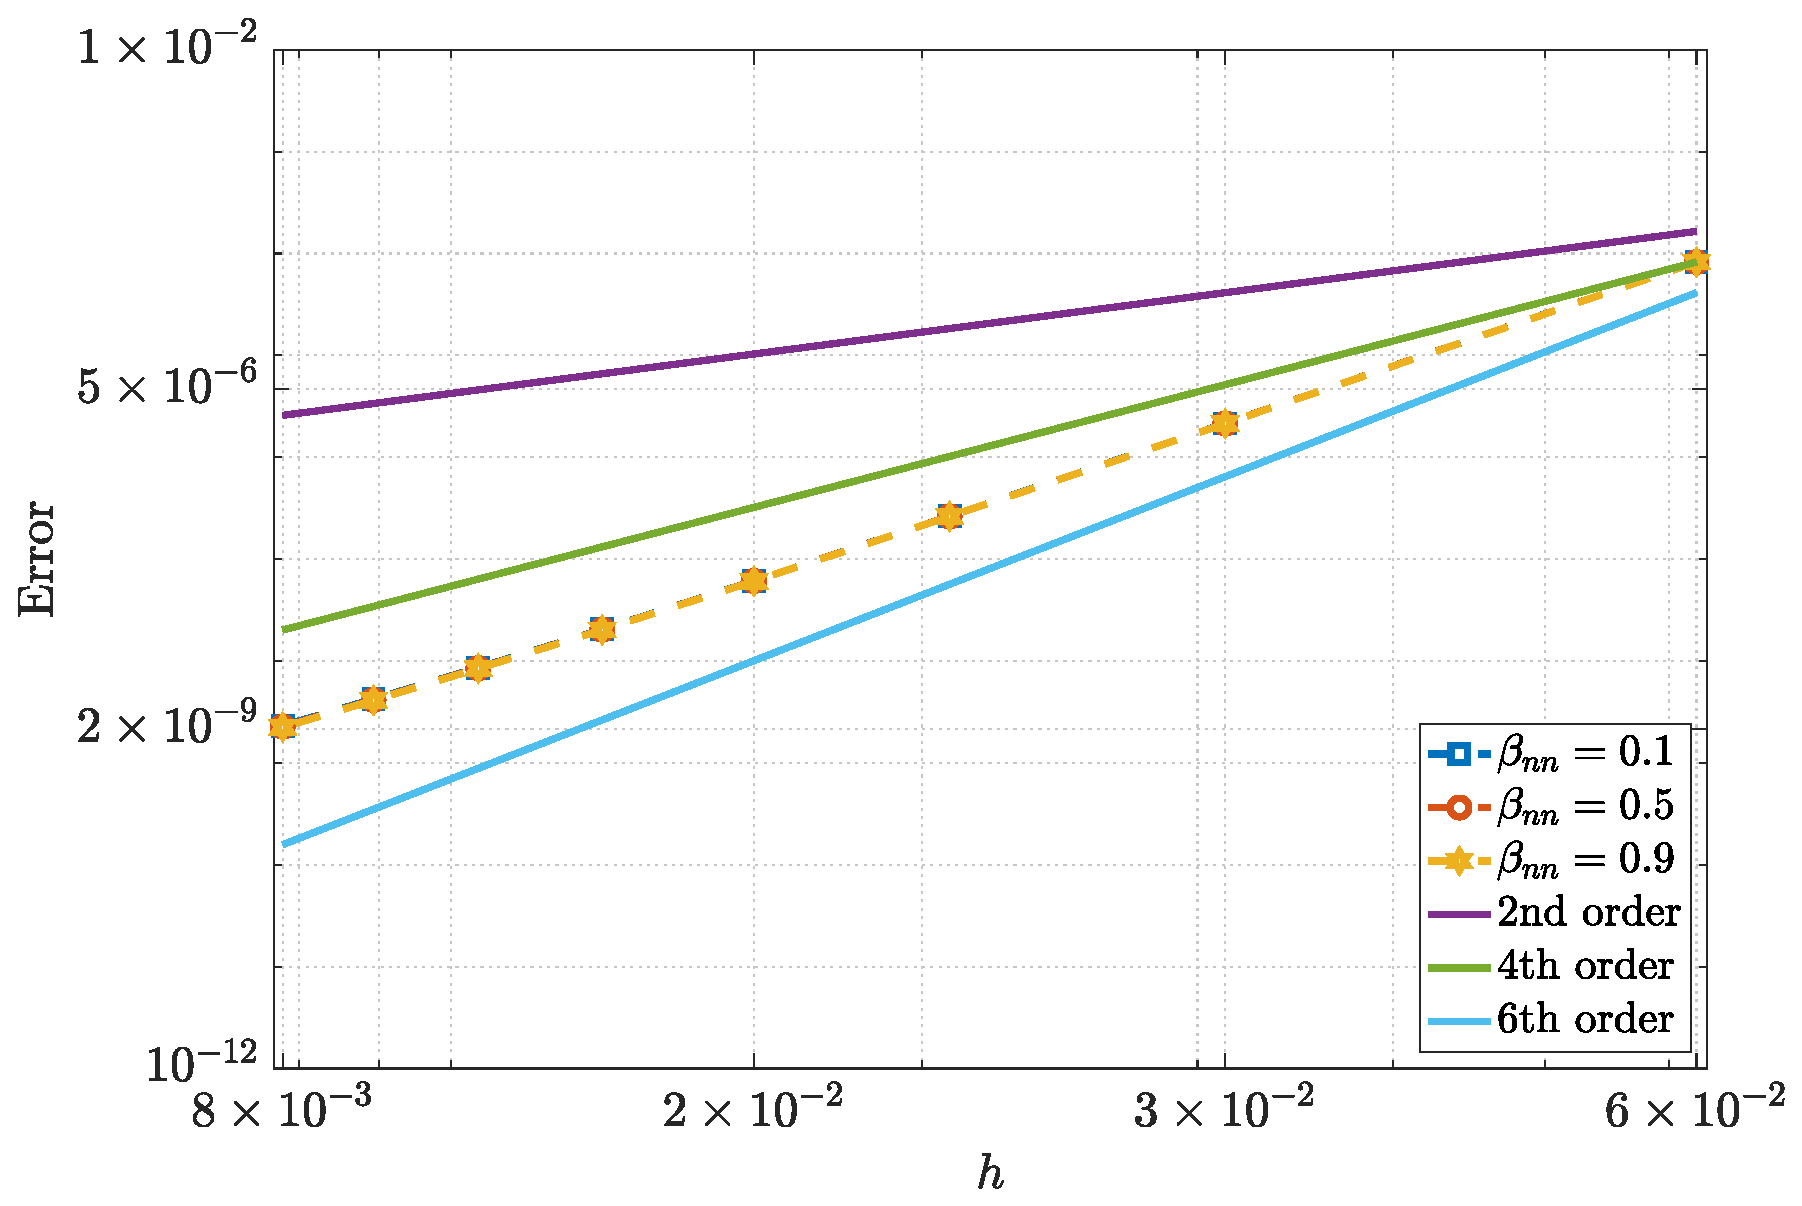
\includegraphics[width=\textwidth]{NormErr_2nd_Re_100_Wi_1_epsilon_0_xi_0_alphaG_0_Dt_1e-06_at_0.05_tipsim_1_MMS_12_U.eps}
        \caption{$||u - \overline{u}||_{2}$}
        \label{error_u_2nd_Case1_oldorydb}
    \end{subfigure}
    \vspace{0.2cm}
    \qquad
    \begin{subfigure}[b]{.46\textwidth}
        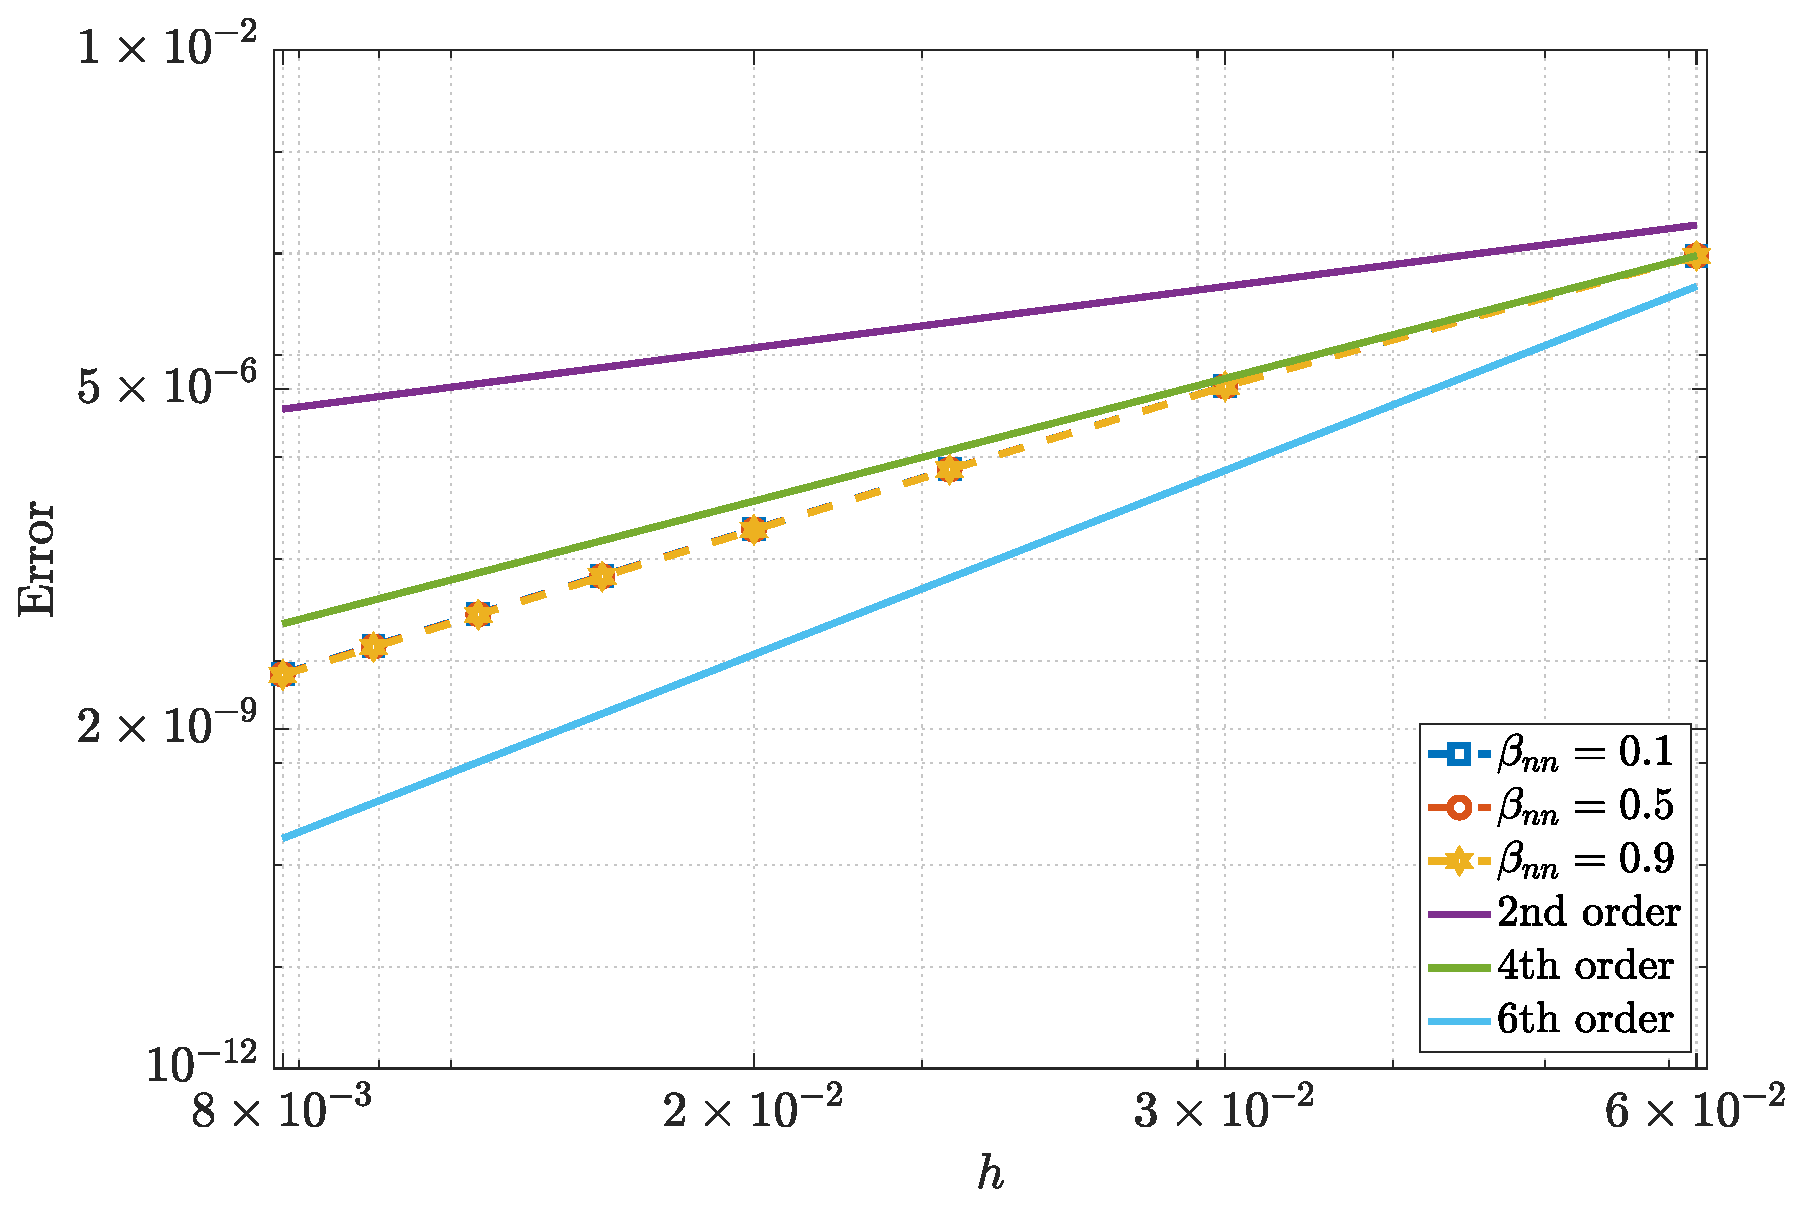
\includegraphics[width=\textwidth]{NormErr_2nd_Re_100_Wi_1_epsilon_0_xi_0_alphaG_0_Dt_1e-06_at_0.05_tipsim_1_MMS_12_V.eps}
        \caption{$||v - \widetilde{v}||_{2}$}
        \label{error_v_2nd_Case1_oldorydb}
    \end{subfigure}
    \qquad
    \begin{subfigure}[b]{.46\textwidth}
        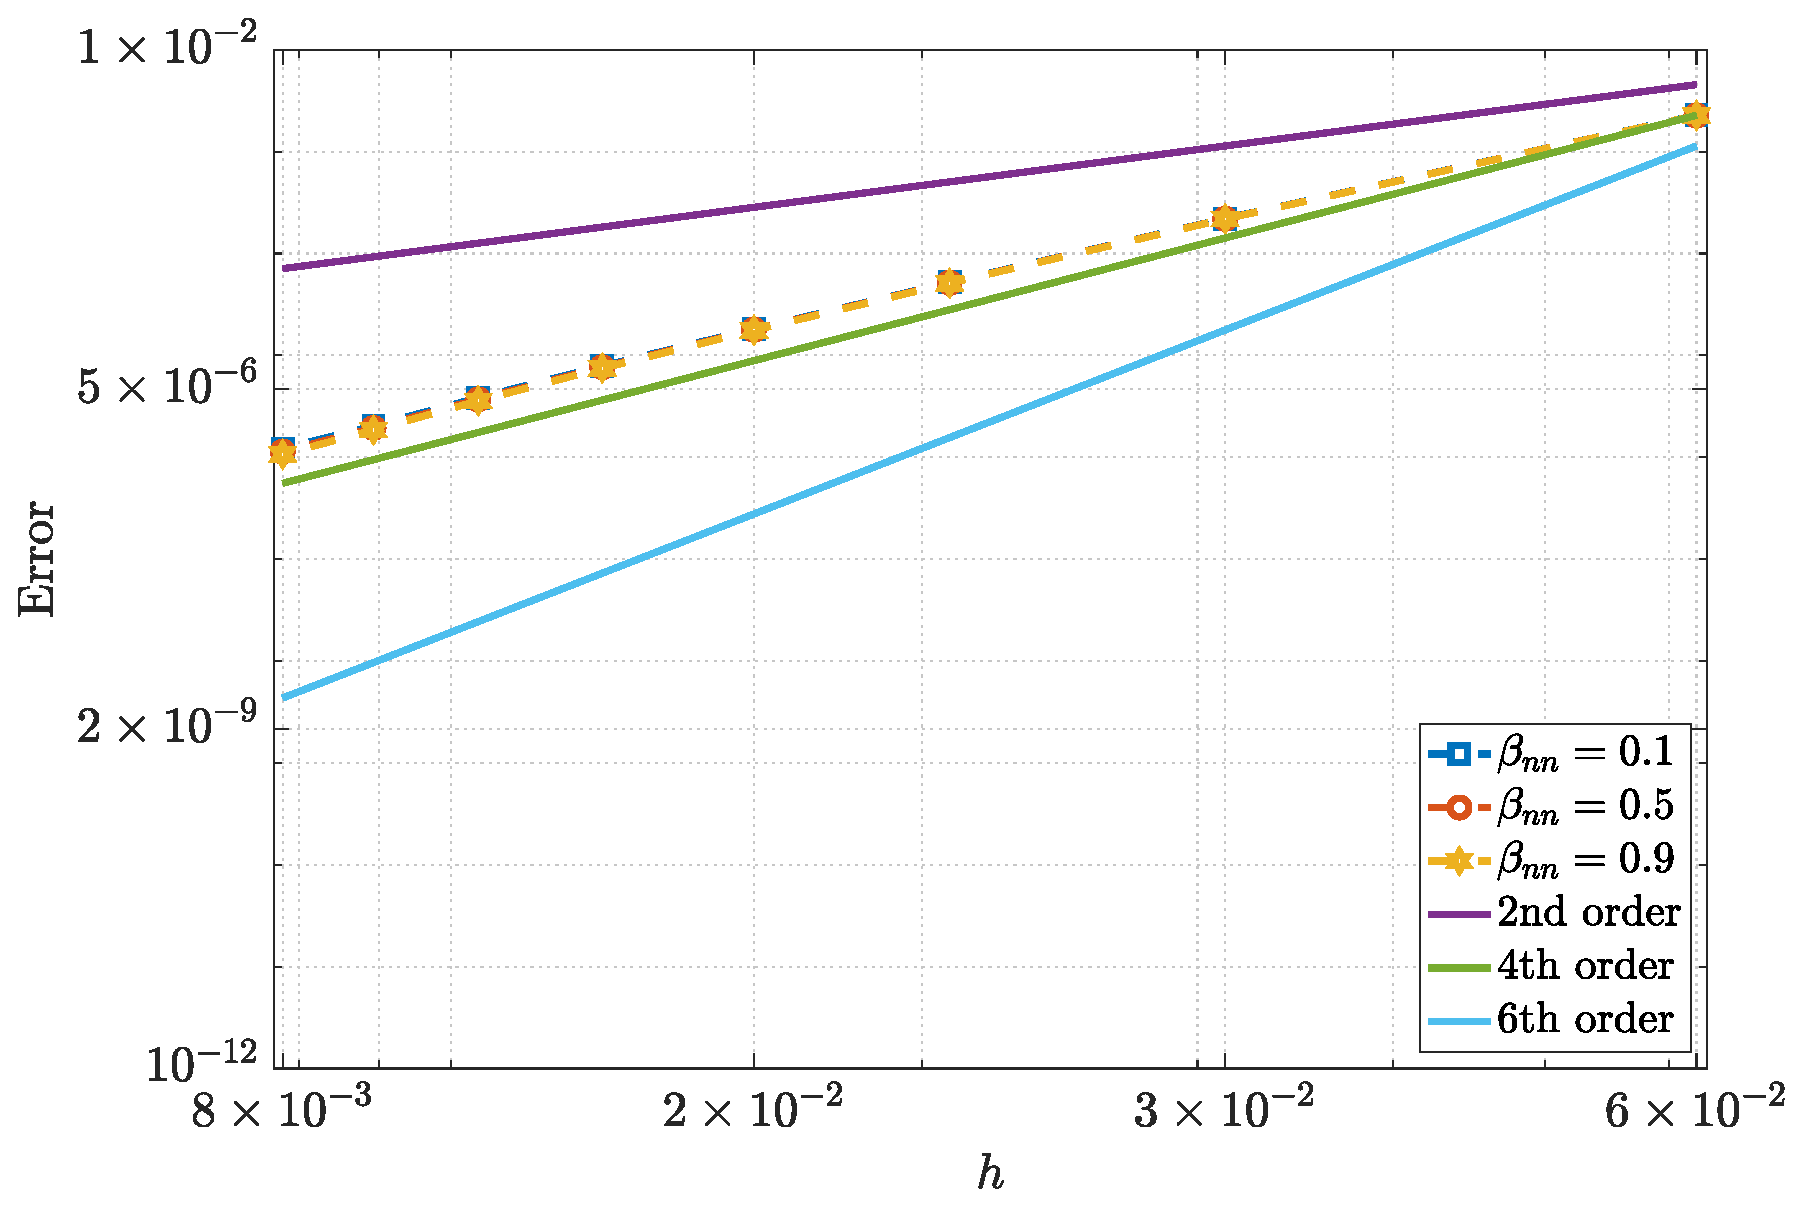
\includegraphics[width=\textwidth]{NormErr_2nd_Re_100_Wi_1_epsilon_0_xi_0_alphaG_0_Dt_1e-06_at_0.05_tipsim_1_MMS_12_Wz.eps}
        \caption{$||\omega_{z} - \widetilde{\omega_{z}}||_{2}$}
        \label{error_wz_2nd_Case1_oldorydb}
    \end{subfigure}
    \vspace{0.02cm}
    \qquad
    \begin{subfigure}[b]{.46\textwidth}
        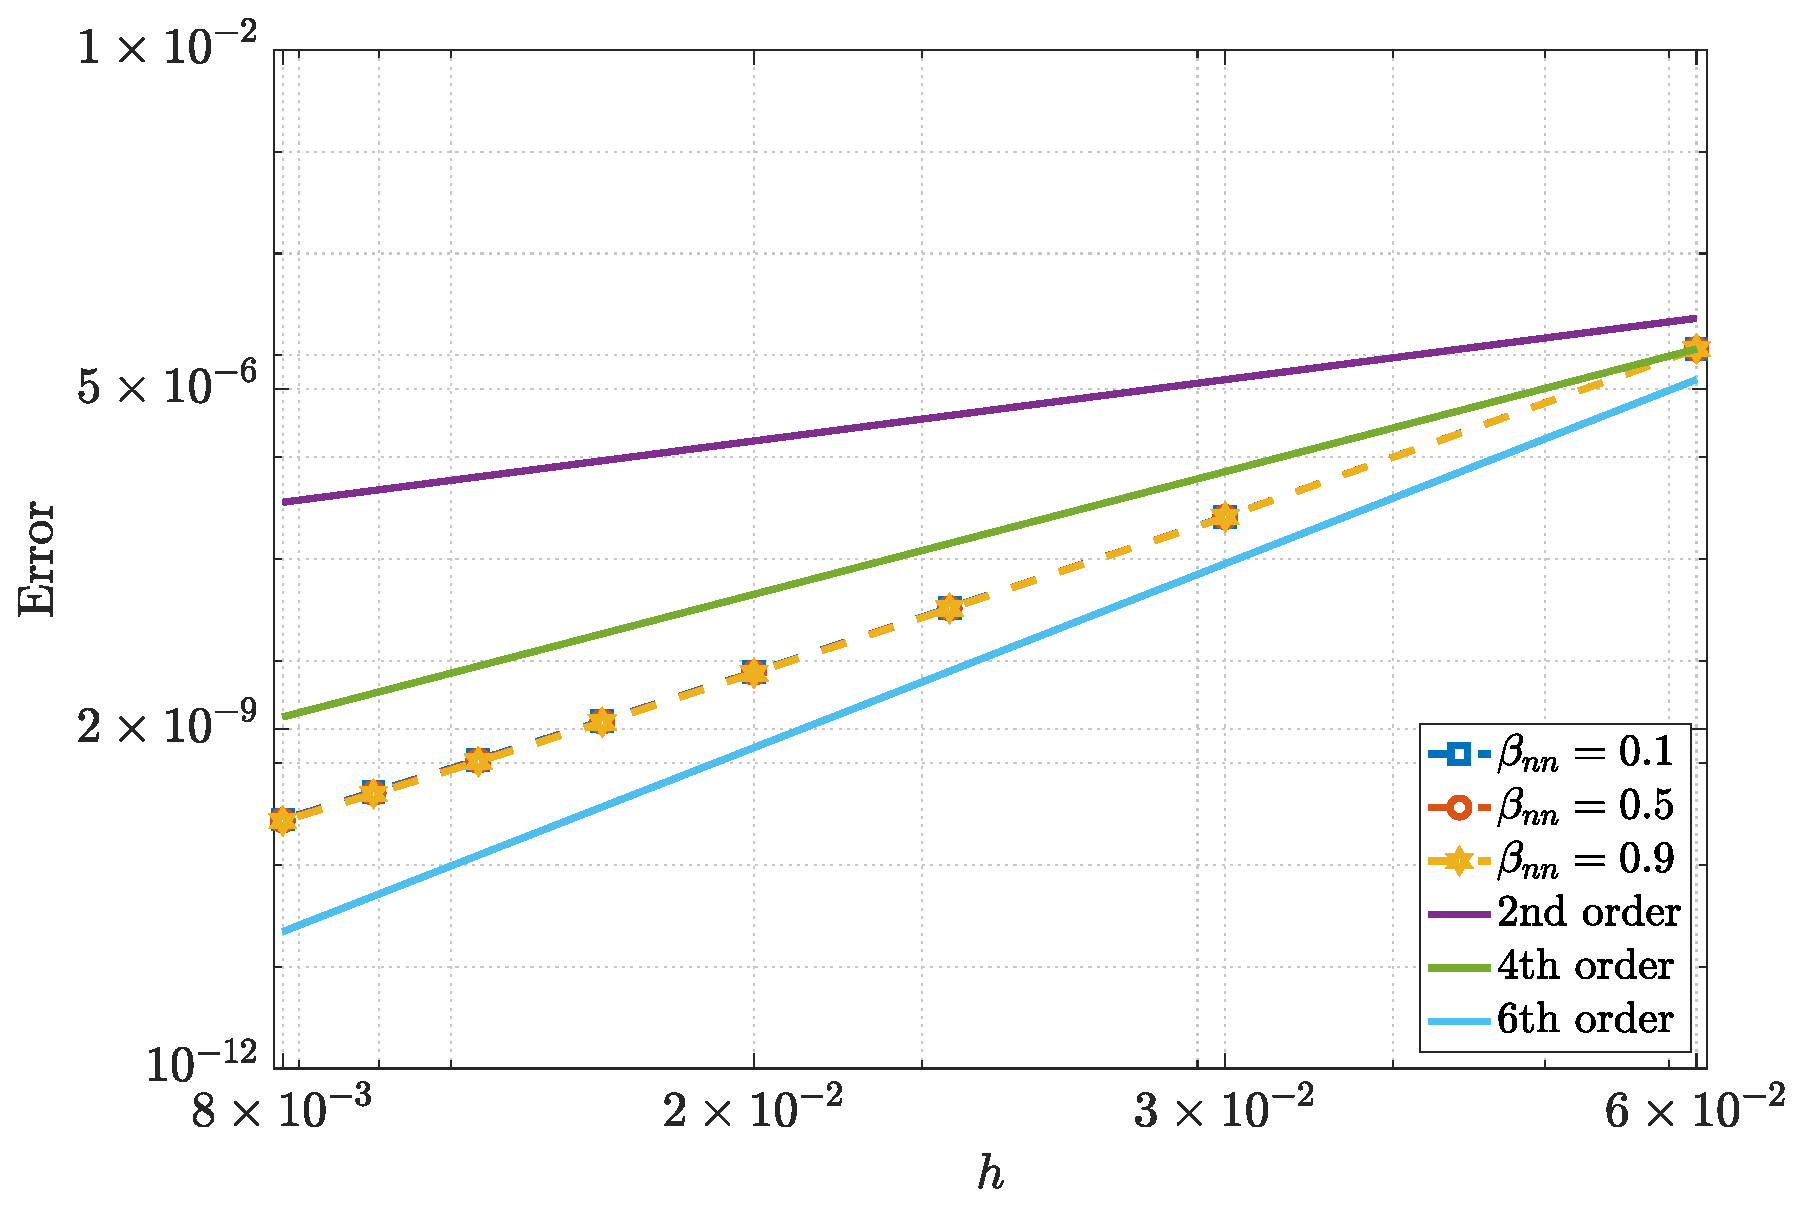
\includegraphics[width=\textwidth]{NormErr_2nd_Re_100_Wi_1_epsilon_0_xi_0_alphaG_0_Dt_1e-06_at_0.05_tipsim_1_MMS_12_Psi.eps}
        \caption{$||\Psi - \widetilde{\Psi}||_{2}$}
        \label{error_psi_2nd_Case1_oldorydb}
    \end{subfigure}
    \vspace{0.02cm}
    \caption{Error for the velocity field $({u},{v})$, vorticity $({\omega_{z}})$, and stream function $({\Psi})$, with $\operatorname{Re}=100$ and $Wi=1$ for the Oldroyd-B viscoelastic fluid flow, using different solvent viscosity ratios ($\beta_{nn}$) and grid sizes ($\Delta x, \Delta y$).\label{fig_OldroydB_error_uvwzpsi}}
\end{figure}

\begin{figure}[H]
    \centering  
    \begin{subfigure}[b]{.46\textwidth}
        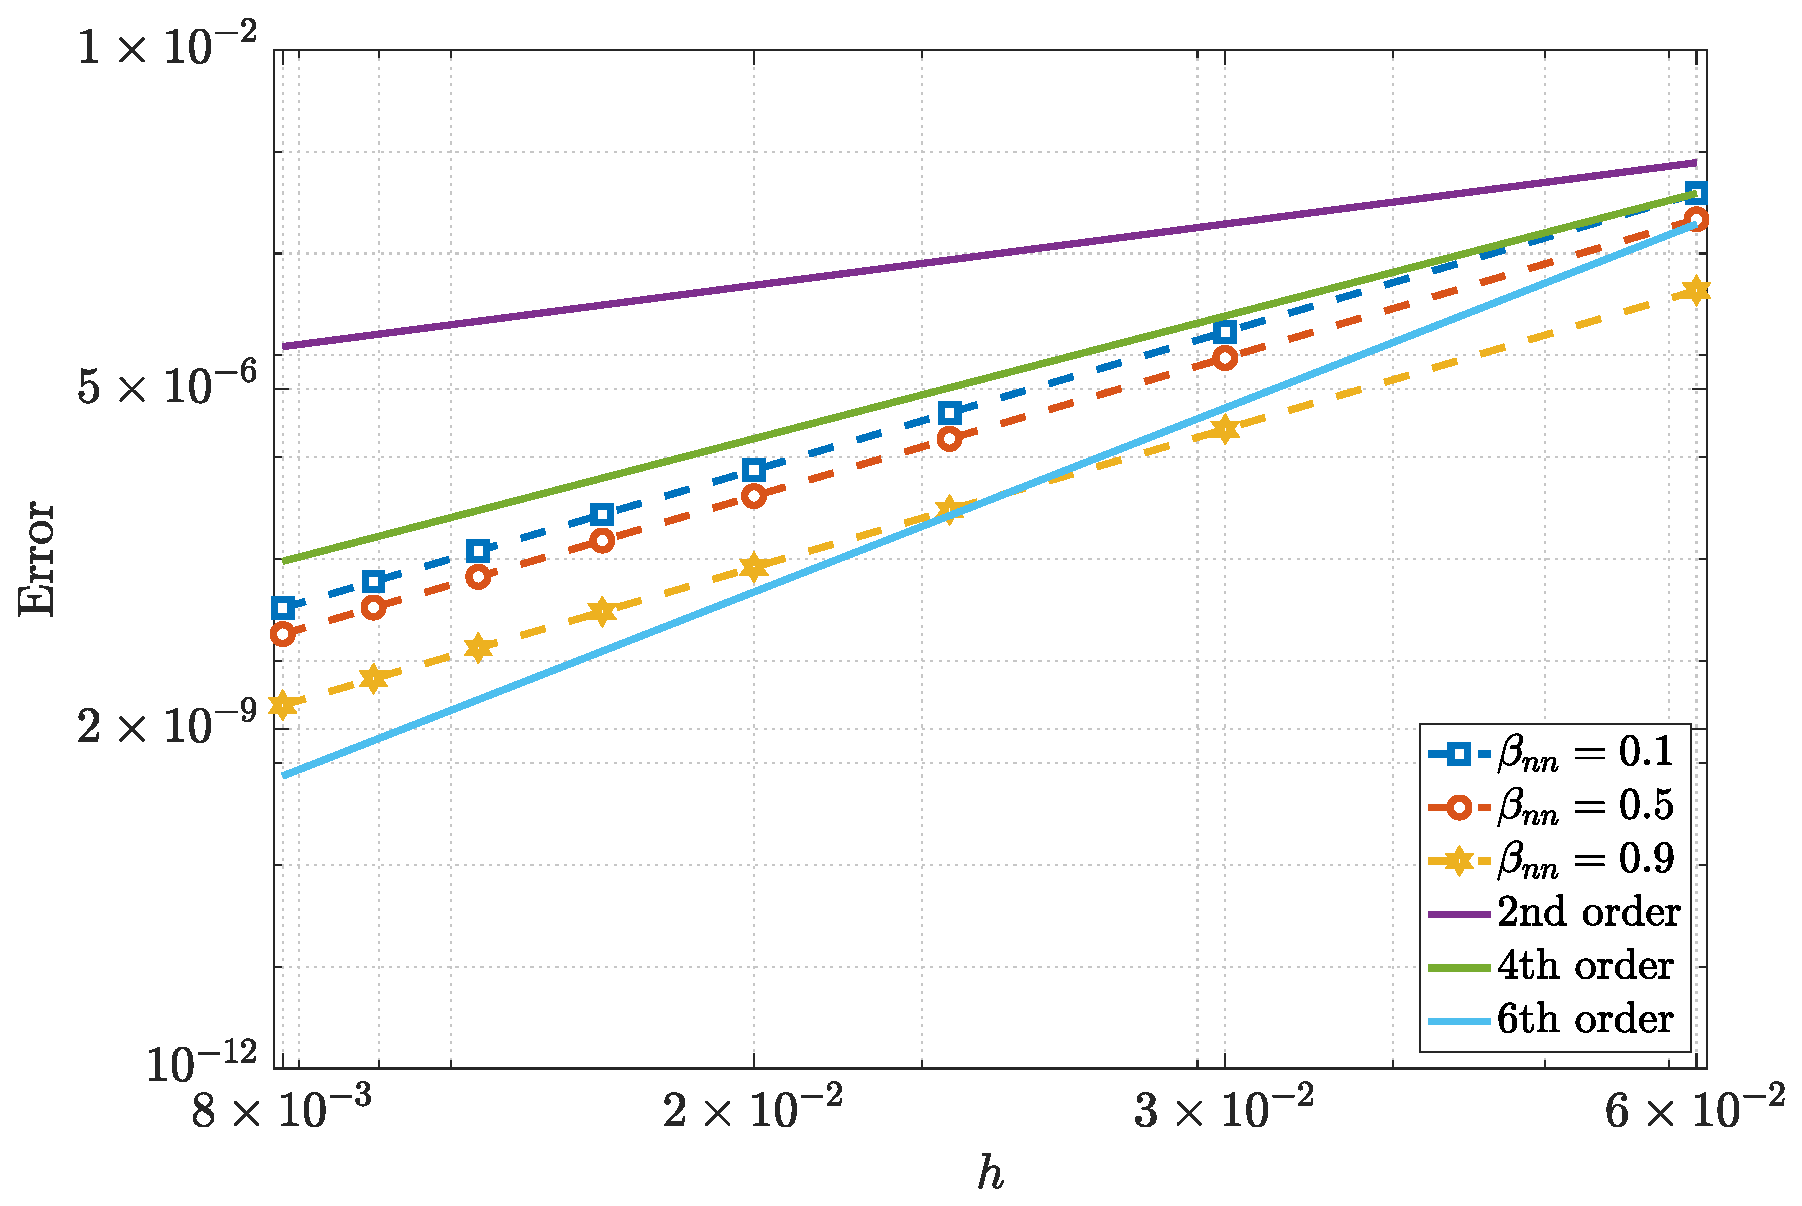
\includegraphics[width=\textwidth]{NormErr_2nd_Re_100_Wi_1_epsilon_0_xi_0_alphaG_0_Dt_1e-06_at_0.05_tipsim_1_MMS_12_Txx.eps}
        \caption{$||T_{xx} - \overline{T}_{xx}||_{2}$}
        \label{error_txx_2nd_Case1_oldorydb}
    \end{subfigure}
    \vspace{0.2cm}
    \qquad
    \begin{subfigure}[b]{.46\textwidth}
        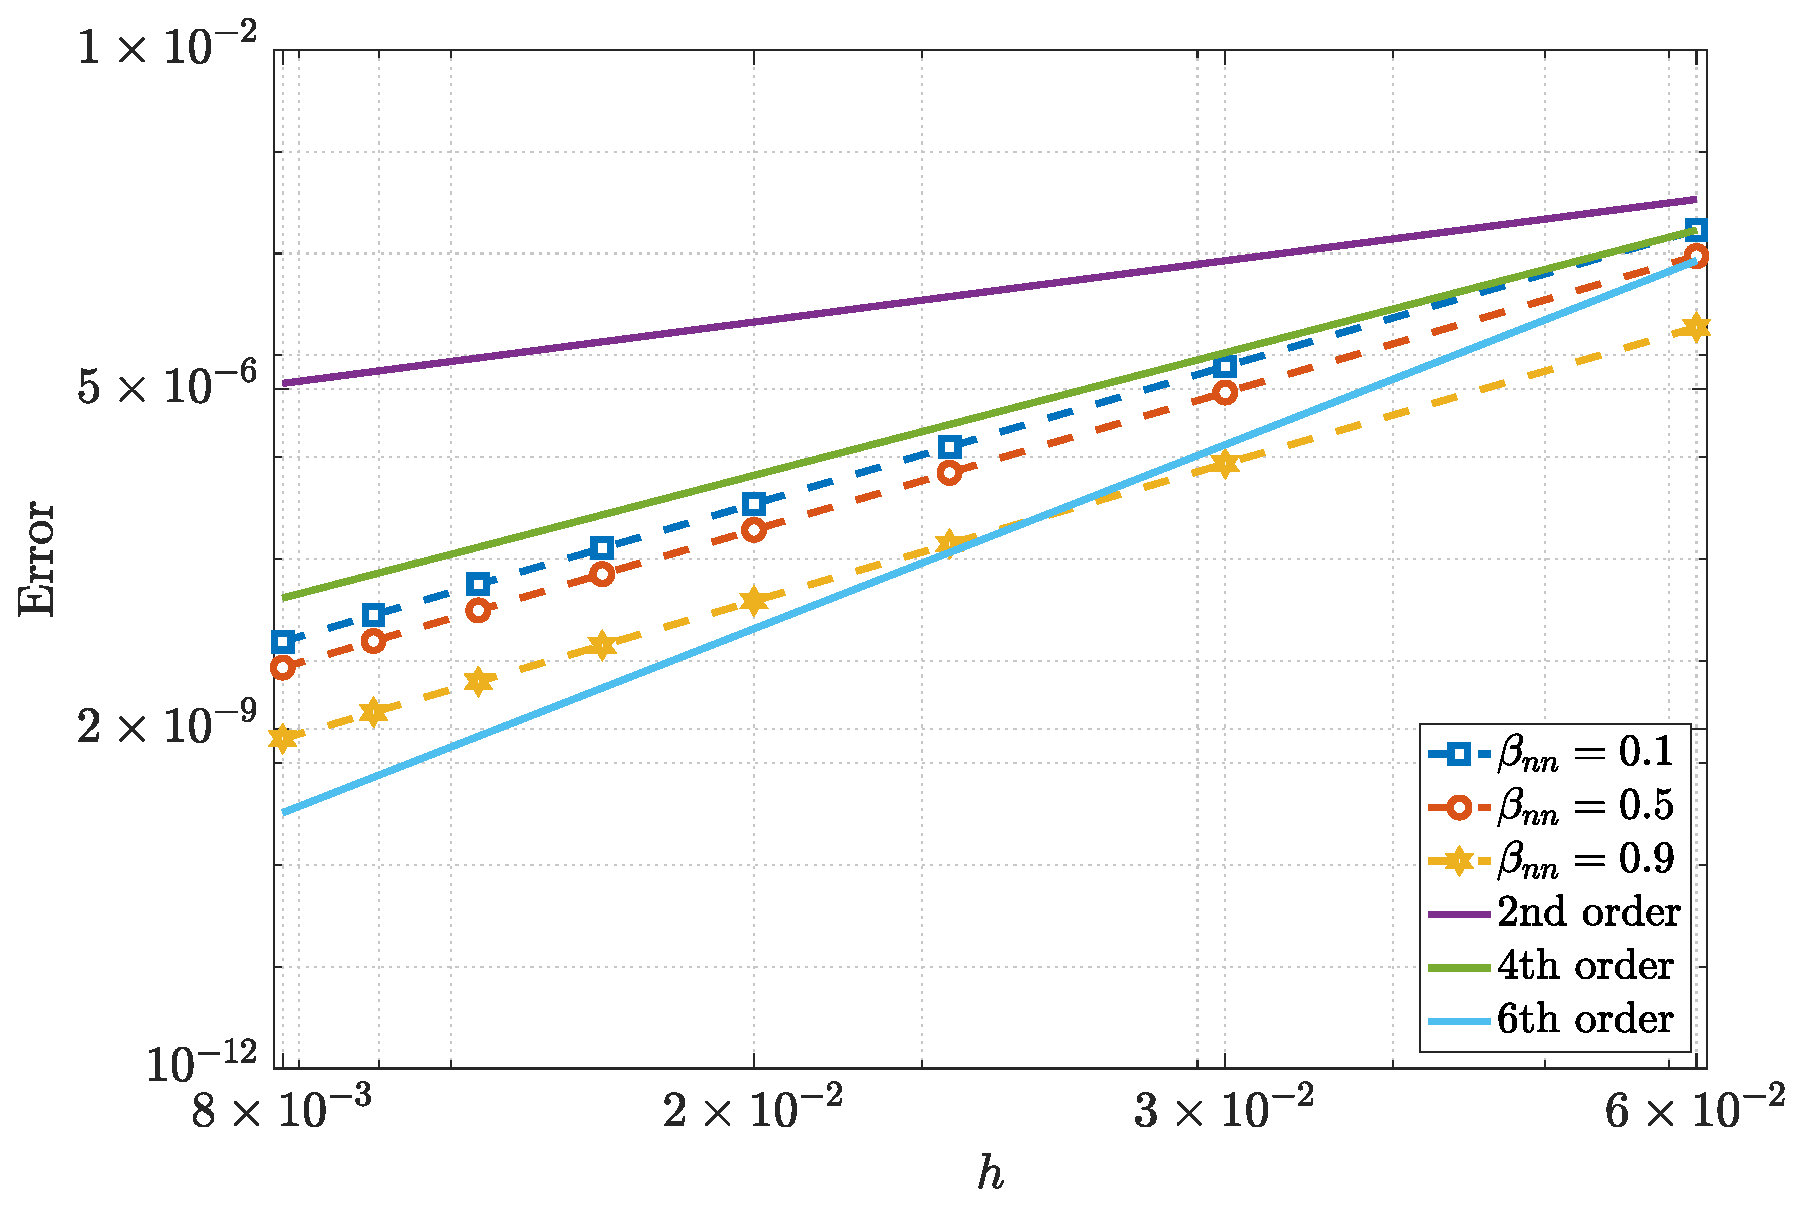
\includegraphics[width=\textwidth]{NormErr_2nd_Re_100_Wi_1_epsilon_0_xi_0_alphaG_0_Dt_1e-06_at_0.05_tipsim_1_MMS_12_Txy.eps}
        \caption{$||T_{xy} - \overline{T}_{xy}||_{2}$}
        \label{error_txy_2nd_Case1_oldorydb}
    \end{subfigure}
    \qquad
    \begin{subfigure}[b]{.46\textwidth}
        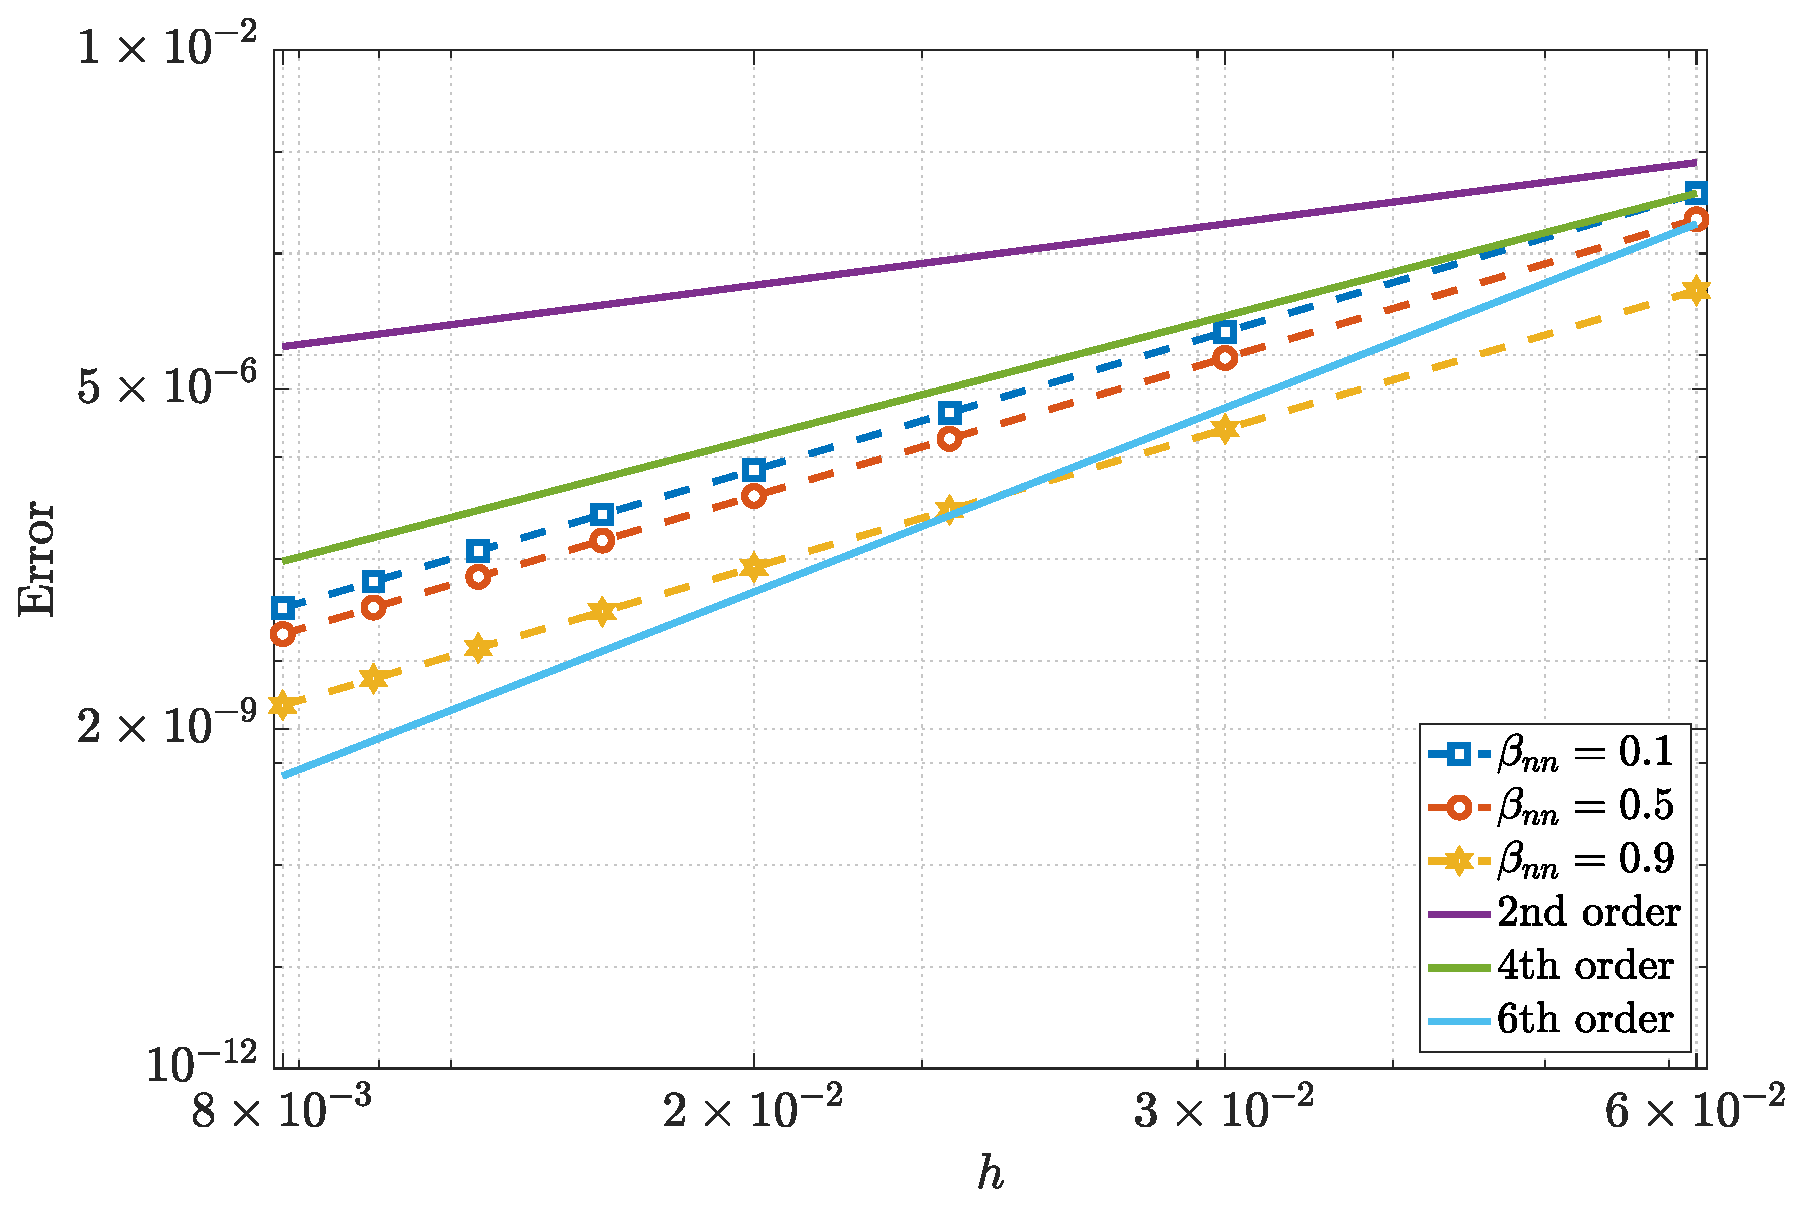
\includegraphics[width=\textwidth]{NormErr_2nd_Re_100_Wi_1_epsilon_0_xi_0_alphaG_0_Dt_1e-06_at_0.05_tipsim_1_MMS_12_Tyy.eps}
        \caption{$||T_{yy} - \overline{T}_{yy}||_{2}$}
        \label{error_tyy_2nd_Case1_oldorydb}
    \end{subfigure}
    \vspace{0.02cm}
    \caption{Error for the polymeric tensor components $({T}_{xx},~{T}_{xy},~{T}_{yy})$, with $\operatorname{Re}=100$ and $Wi=1$ for the Oldroyd-B viscoelastic fluid flow, using different solvent viscosity ratios ($\beta_{nn}$) and grid sizes ($\Delta x, \Delta y$).\label{fig_OldroydB_error_txxxyyy}}
\end{figure}

The results shown in Figures~\ref{fig_OldroydB_error_uvwzpsi} and
\ref{fig_OldroydB_error_txxxyyy}  also compare the theoretical convergence
order (2nd, 4th, and 6th) with the numerical order calculated from the results
obtained by the developed code. The results in
Figure~\ref{fig_OldroydB_error_uvwzpsi} show that the convergence order for
$u$, $v$, $\omega_{z}$, and $\Psi$, across different values of $\beta_{nn}$,
remains similar for each of these solutions, to the point where they overlap.
This indicates that the values of $\beta_{nn}$ do not affect the numerical
resolution obtained and do not influence the convergence order. In
Figure~\ref{fig_OldroydB_error_txxxyyy}, although the errors do not overlap,
they exhibit very similar slopes, indicating that the polymeric tensor
components share a similar convergence order, between 4 and 5. The lack of
overlap is mainly because $\beta_{nn}$ is directly incorporated into the
construction of the manufactured solutions for the polymeric tensor components,
resulting in different initial errors for each solution.

In Table~\ref{tab_OldroydBWzResumida}, the vorticity errors are presented for
$\operatorname{Re}$ of 1, 100, 400, and 1000, using different solvent viscosity
ratios ($\beta_{nn} = 0.1,\ 0.5,\ 0.9,$ and $1.0$). As the mesh is refined,{\color{red} the
results show a consistent reduction in numerical errors, indicating the
robustness of the proposed method. The convergence order generally approaches
the expected value of 4.5 for high-order numerical schemes, particularly for
the velocity and stress components. However, Table~\ref{tab_OldroydBWzResumida}
reveals that the convergence rate for vorticity decreases slightly (to
approximately 3.5–4.0) at higher Reynolds numbers ($\operatorname{Re} \geq
100$). This reduction is attributed to the increasing influence of convective
terms on the vorticity field, which tends to amplify numerical dissipation and
sensitivity to grid resolution. Despite this localized drop in convergence, the
consistency of high-order accuracy across most variables and flow conditions
reinforces the overall robustness and reliability of the numerical model for
simulating nonlinear viscoelastic flows across a broad range of solvent
viscosity ratios and flow regimes.}
\begin{center}
\begin{table}[H]
\caption{Numerical errors and convergence order calculation for vorticity $(\omega_{z})$, using \mbox{$Wi=1$}, $Re=\{1,100,400,1000\}$ and $\beta_{nn}=\{0.1,0.5,0.9,1.0\}$, for the Oldroyd-B viscoelastic fluid flow.\label{tab_OldroydBWzResumida}}
\scriptsize{
    \begin{tabular*}{\textwidth}{@{\extracolsep\fill}cccccccccc@{}}
    \hline
    \multirow{2}{*}{$\operatorname{Re}$} & \multirow{2}{*}{Mesh} & \multicolumn{2}{c}{$\beta_{nn}=0.1$}  & \multicolumn{2}{c}{$\beta_{nn}=0.5$}  & \multicolumn{2}{c}{$\beta_{nn}=0.9$}  & \multicolumn{2}{c}{$\beta_{nn}=1.0$}\\ %\cline{2-10}
     & & Error & Order & Error & Order & Error & Order & Error & Order \\
    \hline
    \multirow{7}{*}{1.00} & $17\times 17$ & 2.23e-03 & --- & 2.08e-03 & --- & 1.96e-03 & --- & 1.93e-03 & --- \\
    & $33\times 33$ & 2.02e-04 & 3.47 & 1.51e-04 & 3.79 & 1.23e-04 & 4.00 & 1.18e-04 & 4.03 \\
    & $49\times 49$ & 4.26e-05 & 3.84 & 2.50e-05 & 4.44 & 1.92e-05 & 4.57 & 1.84e-05 & 4.58 \\
    & $65\times 65$ & 1.28e-05 & 4.17 & 6.43e-06 & 4.71 & 5.05e-06 & 4.65 & 4.85e-06 & 4.63 \\
    & $81\times 81$ & 4.68e-06 & 4.52 & 2.23e-06 & 4.74 & 1.79e-06 & 4.63 & 1.73e-06 & 4.61 \\
    & $97\times 97$ & 1.92e-06 & 4.90 & 9.34e-07 & 4.78 & 7.68e-07 & 4.65 & 7.45e-07 & 4.63 \\
    & $113\times 113$ & 8.58e-07 & 5.21 & 4.47e-07 & 4.77 & 3.80e-07 & 4.57 & 3.71e-07 & 4.52 \\
    & $129\times 129$ & 4.34e-07 & 5.10 & 2.59e-07 & 4.11 & 2.30e-07 & 3.76 & 2.26e-07 & 3.71 \\
    \hline\hline
    \multirow{7}{*}{100.00} & $17\times 17$ & 2.27e-03 & --- & 2.27e-03 & --- & 2.26e-03 & --- & 2.26e-03 & --- \\
    & $33\times 33$ & 2.20e-04 & 3.37 & 2.19e-04 & 3.37 & 2.18e-04 & 3.37 & 2.18e-04 & 3.37 \\
    & $49\times 49$ & 5.20e-05 & 3.56 & 5.15e-05 & 3.57 & 5.11e-05 & 3.58 & 5.10e-05 & 3.59 \\
    & $65\times 65$ & 1.82e-05 & 3.66 & 1.79e-05 & 3.68 & 1.76e-05 & 3.70 & 1.75e-05 & 3.71 \\
    & $81\times 81$ & 7.84e-06 & 3.76 & 7.65e-06 & 3.80 & 7.47e-06 & 3.84 & 7.43e-06 & 3.85 \\
    & $97\times 97$ & 3.83e-06 & 3.93 & 3.70e-06 & 3.99 & 3.57e-06 & 4.05 & 3.54e-06 & 4.06 \\
    & $113\times 113$ & 2.04e-06 & 4.10 & 1.94e-06 & 4.19 & 1.85e-06 & 4.27 & 1.83e-06 & 4.29 \\
    & $129\times 129$ & 1.21e-06 & 3.89 & 1.13e-06 & 4.02 & 1.07e-06 & 4.13 & 1.05e-06 & 4.16 \\
    \hline\hline
    \multirow{7}{*}{400.00} & $17\times 17$ & 2.27e-03 & --- & 2.27e-03 & --- & 2.27e-03 & --- & 2.27e-03 & --- \\
    & $33\times 33$ & 2.20e-04 & 3.37 & 2.20e-04 & 3.37 & 2.20e-04 & 3.37 & 2.20e-04 & 3.37 \\
    & $49\times 49$ & 5.21e-05 & 3.56 & 5.19e-05 & 3.56 & 5.18e-05 & 3.56 & 5.18e-05 & 3.56 \\
    & $65\times 65$ & 1.82e-05 & 3.65 & 1.81e-05 & 3.66 & 1.81e-05 & 3.66 & 1.81e-05 & 3.66 \\
    & $81\times 81$ & 7.88e-06 & 3.75 & 7.83e-06 & 3.76 & 7.79e-06 & 3.77 & 7.78e-06 & 3.77 \\
    & $97\times 97$ & 3.86e-06 & 3.92 & 3.83e-06 & 3.93 & 3.80e-06 & 3.94 & 3.79e-06 & 3.95 \\
    & $113\times 113$ & 2.05e-06 & 4.09 & 2.03e-06 & 4.11 & 2.01e-06 & 4.12 & 2.01e-06 & 4.13 \\
    & $129\times 129$ & 1.23e-06 & 3.86 & 1.21e-06 & 3.89 & 1.19e-06 & 3.92 & 1.19e-06 & 3.93 \\
    \hline\hline
    \multirow{7}{*}{1000.00} & $17\times 17$ & 2.27e-03 & --- & 2.27e-03 & --- & 2.27e-03 & --- & 2.27e-03 & --- \\
    & $33\times 33$ & 2.20e-04 & 3.37 & 2.20e-04 & 3.37 & 2.20e-04 & 3.37 & 2.20e-04 & 3.37 \\
    & $49\times 49$ & 5.21e-05 & 3.56 & 5.20e-05 & 3.56 & 5.20e-05 & 3.56 & 5.20e-05 & 3.56 \\
    & $65\times 65$ & 1.82e-05 & 3.65 & 1.82e-05 & 3.65 & 1.82e-05 & 3.65 & 1.82e-05 & 3.65 \\
    & $81\times 81$ & 7.89e-06 & 3.75 & 7.87e-06 & 3.76 & 7.86e-06 & 3.76 & 7.85e-06 & 3.76 \\
    & $97\times 97$ & 3.86e-06 & 3.92 & 3.85e-06 & 3.92 & 3.84e-06 & 3.92 & 3.84e-06 & 3.92 \\
    & $113\times 113$ & 2.06e-06 & 4.08 & 2.05e-06 & 4.09 & 2.04e-06 & 4.09 & 2.04e-06 & 4.09 \\
    & $129\times 129$ & 1.23e-06 & 3.86 & 1.22e-06 & 3.87 & 1.22e-06 & 3.87 & 1.22e-06 & 3.88 \\
    \hline
    \end{tabular*}
}
\end{table}
\end{center}

\begin{center}
\begin{table}[H]
\caption{Numerical errors and convergence order calculation for polymeric tensor component $T_{xx}$, using $Wi=1$, $Re=\{1,100,400,1000\}$ and $\beta_{nn}=\{0.1,0.5,0.9,1.0\}$, for the Oldroyd-B viscoelastic fluid flow.\label{tab_OldroydBTxxResumida}}
\scriptsize{
    \begin{tabular*}{\textwidth}{@{\extracolsep\fill}cccccccccc@{}}
    \hline
    \multirow{2}{*}{$\operatorname{Re}$} & \multirow{2}{*}{Mesh} & \multicolumn{2}{c}{$\beta_{nn}=0.1$}  & \multicolumn{2}{c}{$\beta_{nn}=0.5$}  & \multicolumn{2}{c}{$\beta_{nn}=0.9$}  & \multicolumn{2}{c}{$\beta_{nn}=1.0$}\\ %\cline{3-10}
     & & Error & Order & Error & Order & Error & Order & Error & Order \\
    \hline
    \multirow{7}{*}{1.00} & $17\times 17$ & 3.90e-04 & --- & 2.16e-04 & --- & 4.33e-05 & --- & 4.33e-18 & --- \\
    & $33\times 33$ & 1.70e-05 & 4.52 & 9.42e-06 & 4.52 & 1.88e-06 & 4.52 & 1.88e-19 & 4.52 \\
    & $49\times 49$ & 2.73e-06 & 4.51 & 1.52e-06 & 4.51 & 3.03e-07 & 4.51 & 3.03e-20 & 4.51 \\
    & $65\times 65$ & 7.48e-07 & 4.50 & 4.15e-07 & 4.50 & 8.31e-08 & 4.50 & 8.30e-21 & 4.50 \\
    & $81\times 81$ & 2.74e-07 & 4.50 & 1.52e-07 & 4.50 & 3.04e-08 & 4.50 & 3.04e-21 & 4.50 \\
    & $97\times 97$ & 1.21e-07 & 4.50 & 6.70e-08 & 4.50 & 1.34e-08 & 4.50 & 1.34e-21 & 4.50 \\
    & $113\times 113$ & 6.03e-08 & 4.50 & 3.35e-08 & 4.50 & 6.70e-09 & 4.50 & 6.69e-22 & 4.50 \\
    & $129\times 129$ & 3.30e-08 & 4.50 & 1.84e-08 & 4.50 & 3.67e-09 & 4.50 & 3.67e-22 & 4.50 \\
    \hline\hline
    \multirow{7}{*}{100.00} & $17\times 17$ & 3.90e-04 & --- & 2.16e-04 & --- & 4.33e-05 & --- & 4.33e-18 & --- \\
    & $33\times 33$ & 1.70e-05 & 4.52 & 9.42e-06 & 4.52 & 1.88e-06 & 4.52 & 1.88e-19 & 4.52 \\
    & $49\times 49$ & 2.73e-06 & 4.51 & 1.52e-06 & 4.51 & 3.03e-07 & 4.51 & 3.03e-20 & 4.51 \\
    & $65\times 65$ & 7.48e-07 & 4.50 & 4.15e-07 & 4.50 & 8.31e-08 & 4.50 & 8.30e-21 & 4.50 \\
    & $81\times 81$ & 2.74e-07 & 4.50 & 1.52e-07 & 4.50 & 3.04e-08 & 4.50 & 3.04e-21 & 4.50 \\
    & $97\times 97$ & 1.21e-07 & 4.50 & 6.70e-08 & 4.50 & 1.34e-08 & 4.50 & 1.34e-21 & 4.50 \\
    & $113\times 113$ & 6.03e-08 & 4.50 & 3.35e-08 & 4.50 & 6.70e-09 & 4.50 & 6.69e-22 & 4.50 \\
    & $129\times 129$ & 3.30e-08 & 4.50 & 1.84e-08 & 4.50 & 3.67e-09 & 4.50 & 3.67e-22 & 4.50 \\
    \hline\hline
    \multirow{7}{*}{400.00} & $17\times 17$ & 3.90e-04 & --- & 2.16e-04 & --- & 4.33e-05 & --- & 4.33e-18 & --- \\
    & $33\times 33$ & 1.70e-05 & 4.52 & 9.42e-06 & 4.52 & 1.88e-06 & 4.52 & 1.88e-19 & 4.52 \\
    & $49\times 49$ & 2.73e-06 & 4.51 & 1.52e-06 & 4.51 & 3.03e-07 & 4.51 & 3.03e-20 & 4.51 \\
    & $65\times 65$ & 7.48e-07 & 4.50 & 4.15e-07 & 4.50 & 8.31e-08 & 4.50 & 8.30e-21 & 4.50 \\
    & $81\times 81$ & 2.74e-07 & 4.50 & 1.52e-07 & 4.50 & 3.04e-08 & 4.50 & 3.04e-21 & 4.50 \\
    & $97\times 97$ & 1.21e-07 & 4.50 & 6.70e-08 & 4.50 & 1.34e-08 & 4.50 & 1.34e-21 & 4.50 \\
    & $113\times 113$ & 6.03e-08 & 4.50 & 3.35e-08 & 4.50 & 6.70e-09 & 4.50 & 6.69e-22 & 4.50 \\
    & $129\times 129$ & 3.30e-08 & 4.50 & 1.84e-08 & 4.50 & 3.67e-09 & 4.50 & 3.67e-22 & 4.50 \\
    \hline\hline
    \multirow{7}{*}{1000.00} & $17\times 17$ & 3.90e-04 & --- & 2.16e-04 & --- & 4.33e-05 & --- & 4.33e-18 & --- \\
    & $33\times 33$ & 1.70e-05 & 4.52 & 9.42e-06 & 4.52 & 1.88e-06 & 4.52 & 1.88e-19 & 4.52 \\
    & $49\times 49$ & 2.73e-06 & 4.51 & 1.52e-06 & 4.51 & 3.03e-07 & 4.51 & 3.03e-20 & 4.51 \\
    & $65\times 65$ & 7.48e-07 & 4.50 & 4.15e-07 & 4.50 & 8.31e-08 & 4.50 & 8.30e-21 & 4.50 \\
    & $81\times 81$ & 2.74e-07 & 4.50 & 1.52e-07 & 4.50 & 3.04e-08 & 4.50 & 3.04e-21 & 4.50 \\
    & $97\times 97$ & 1.21e-07 & 4.50 & 6.70e-08 & 4.50 & 1.34e-08 & 4.50 & 1.34e-21 & 4.50 \\
    & $113\times 113$ & 6.03e-08 & 4.50 & 3.35e-08 & 4.50 & 6.70e-09 & 4.50 & 6.69e-22 & 4.50 \\
    & $129\times 129$ & 3.30e-08 & 4.50 & 1.84e-08 & 4.50 & 3.67e-09 & 4.50 & 3.67e-22 & 4.50 \\
    \hline
    \end{tabular*}
}
\end{table}
\end{center}

Table~\ref{tab_OldroydBTxxResumida} presents the errors and convergence orders
for the $T_{xx}$ component of the polymeric stress tensor. Similarly to the
vorticity results, a clear reduction in errors is observed as the mesh is
refined, with the convergence order remaining close to 4.5 under all evaluated
conditions. These results indicate the stability and robustness of the
numerical method in the simulation of both vorticity and polymeric tensor
components. When examining Table~\ref{tab_OldroydBTxxResumida} for $\beta_{nn}
= 1$, it is evident that the numerical errors are extremely small, approaching
the machine precision levels (e.g. $5.97e{-18}$ or $4.94e{-22}$). This
behaviour is expected since $\beta_{nn} = 1$ corresponds to the case of a
Newtonian fluid, where polymeric tensor components such as $T_{xx}$ become
negligible. As a result, the errors are minimal and the convergence order
remains consistently around $4.5$, aligning with the performance of high-order
numerical methods. The negligible errors for $\beta_{nn} = 1$ demonstrate that
the numerical scheme accurately captures the limiting case of a Newtonian fluid
with high precision.

To illustrate the key characteristics of the numerical solutions obtained from
the code developed, profiles are taken at $x=0.25$, $x=0.75$, $y=0.25$, and
$y=0.75$, marked red and blue, respectively, in Figure~\ref{fig_domain}.
Figures \ref{fig_slice_Solution_uvwzpsi_oldroydb_x} and
\ref{fig_slice_Solution_uvwzpsi_oldroydb_y} display profiles of the velocity
field components $(u, v)$, vorticity $(\omega_z)$, and the stream function
$(\Psi)$ along the lines $x=0.25$ and $y=0.75$, respectively, for the Oldroyd-B
constitutive model, under the conditions of $\operatorname{Re}=1000$ and
$Wi=1$. In this context, the continuous lines represent the manufactured
solutions, while the markers correspond to the numerical solutions, both
computed under the same parameters. These profiles will enable visualization of
the behaviour of the velocity components, the vorticity, and the polymeric
tensor components.
\begin{figure}[H]
    \centering
    \begin{subfigure}[b]{.46\textwidth}
        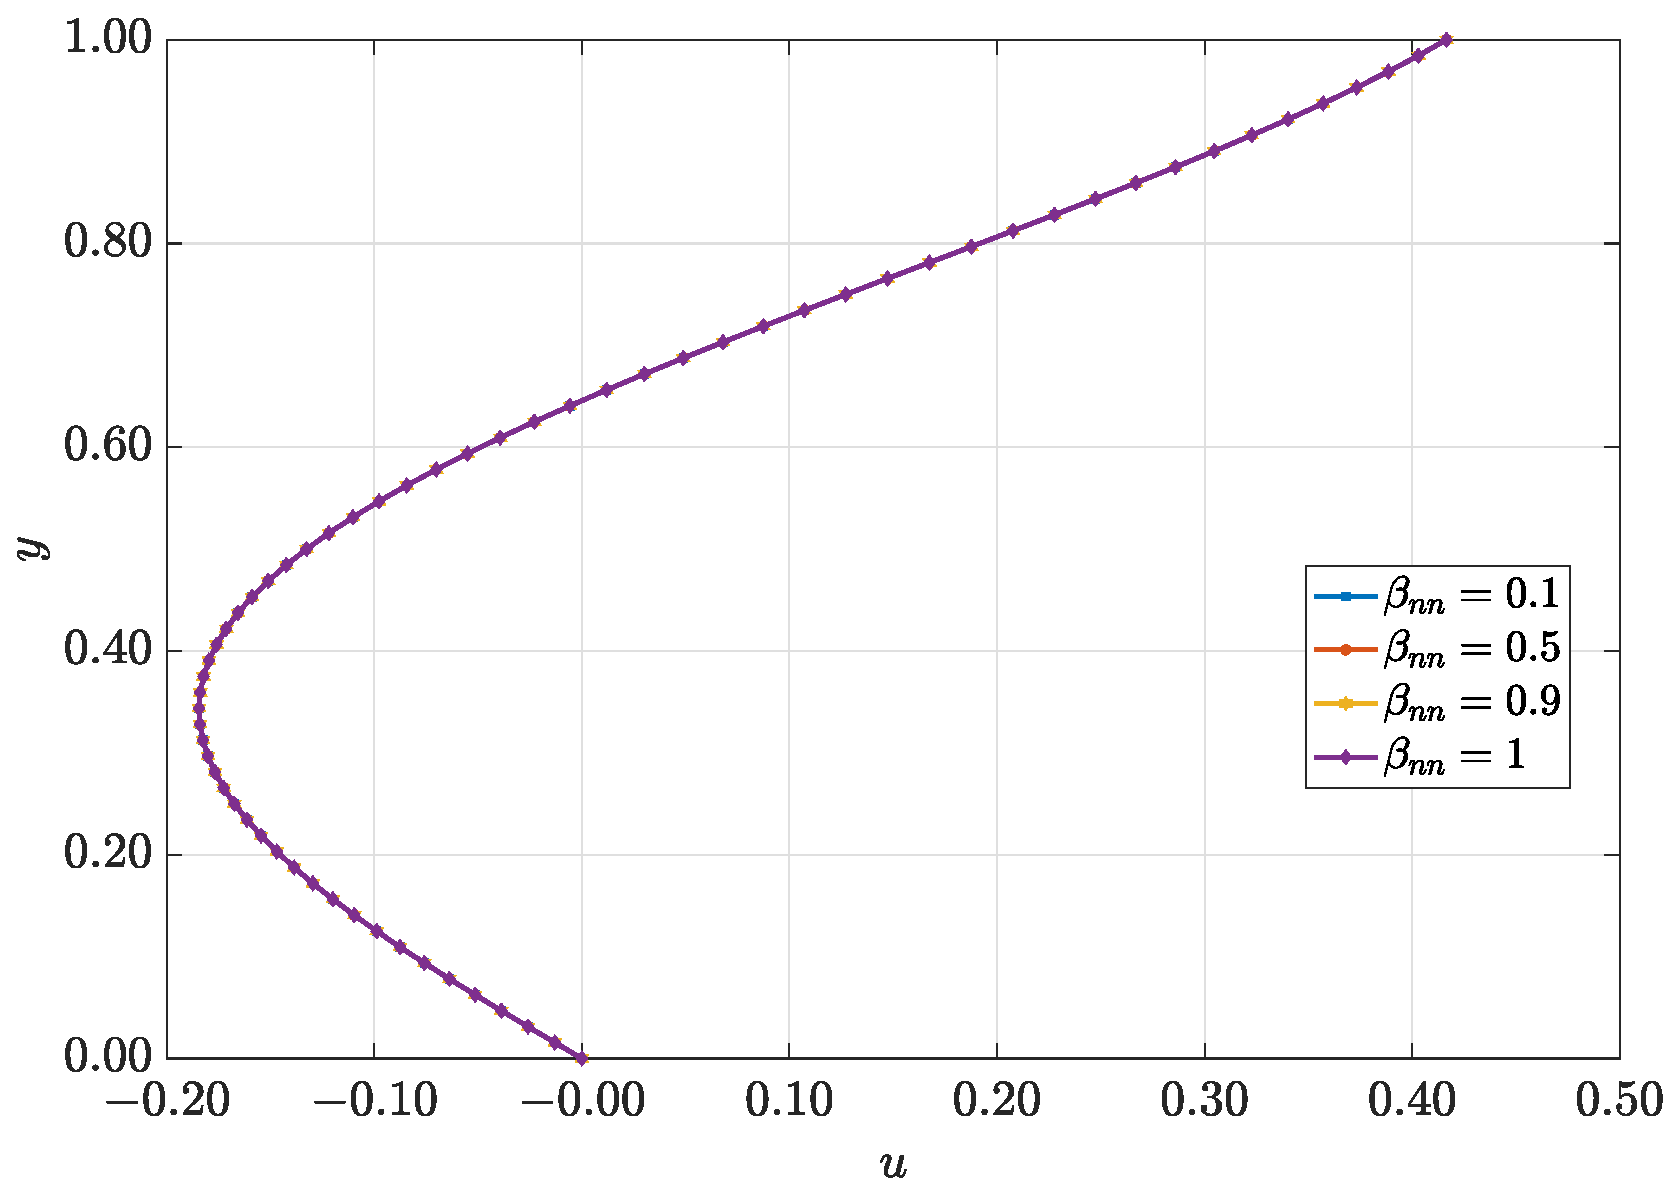
\includegraphics[width=\textwidth]{Slice_x_Tog_Numerical_NormErr_2nd_Betann_1_Re_1000_Wi_1_epsilon_0_xi_0_alphaG_0_Dt_1e-06_at_0.05_tipsim_1_MMS_12_x0.25y0.25_U.eps}
        \caption{Profile at $x=0.25$ for the velocity field component $(u)$}
        \label{fig_slice_x_u_2nd_Case1_oldroydB}
    \end{subfigure}
    \vspace{0.2cm}
    \qquad
    \begin{subfigure}[b]{.46\textwidth}
        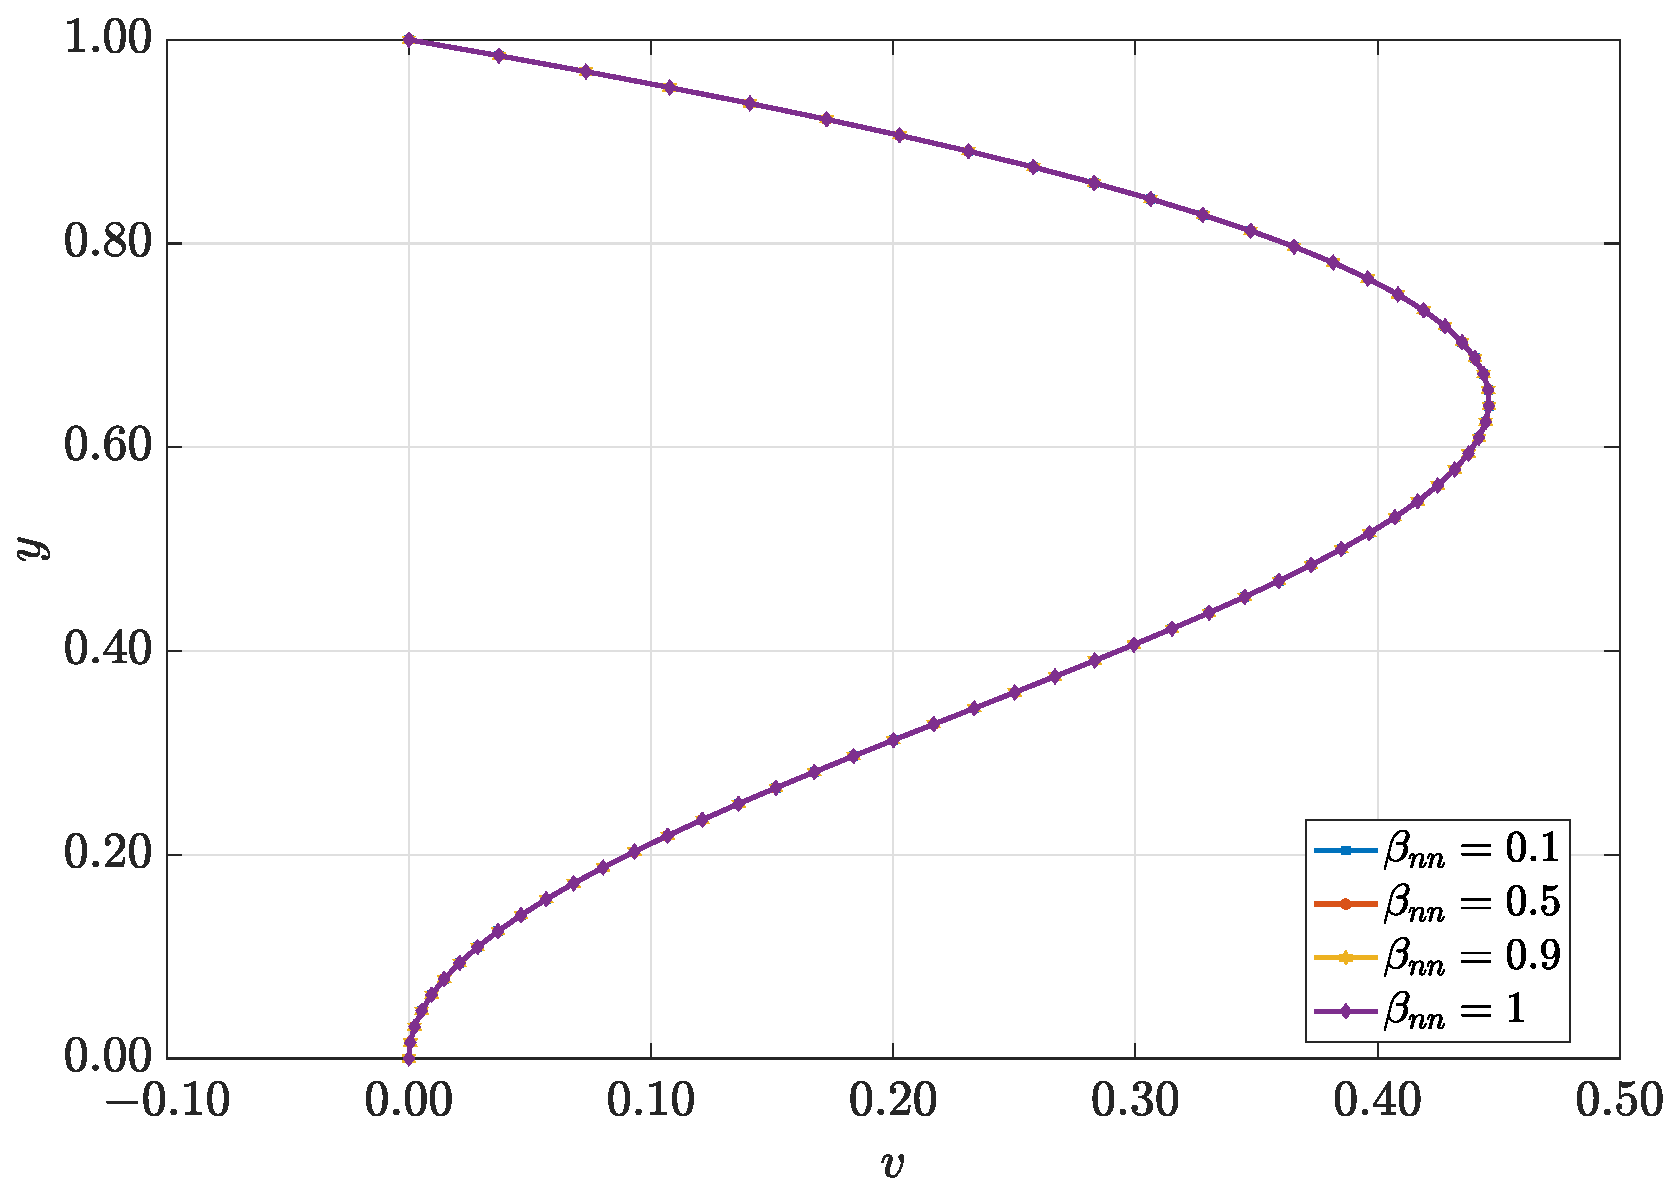
\includegraphics[width=\textwidth]{Slice_x_Tog_Numerical_NormErr_2nd_Betann_1_Re_1000_Wi_1_epsilon_0_xi_0_alphaG_0_Dt_1e-06_at_0.05_tipsim_1_MMS_12_x0.25y0.25_V.eps}
        \caption{Profile at $x=0.25$ for the velocity field component $(v)$}
        \label{fig_slice_x_v_2nd_Case1_oldorydb}
    \end{subfigure}
    \begin{subfigure}[b]{.46\textwidth}
        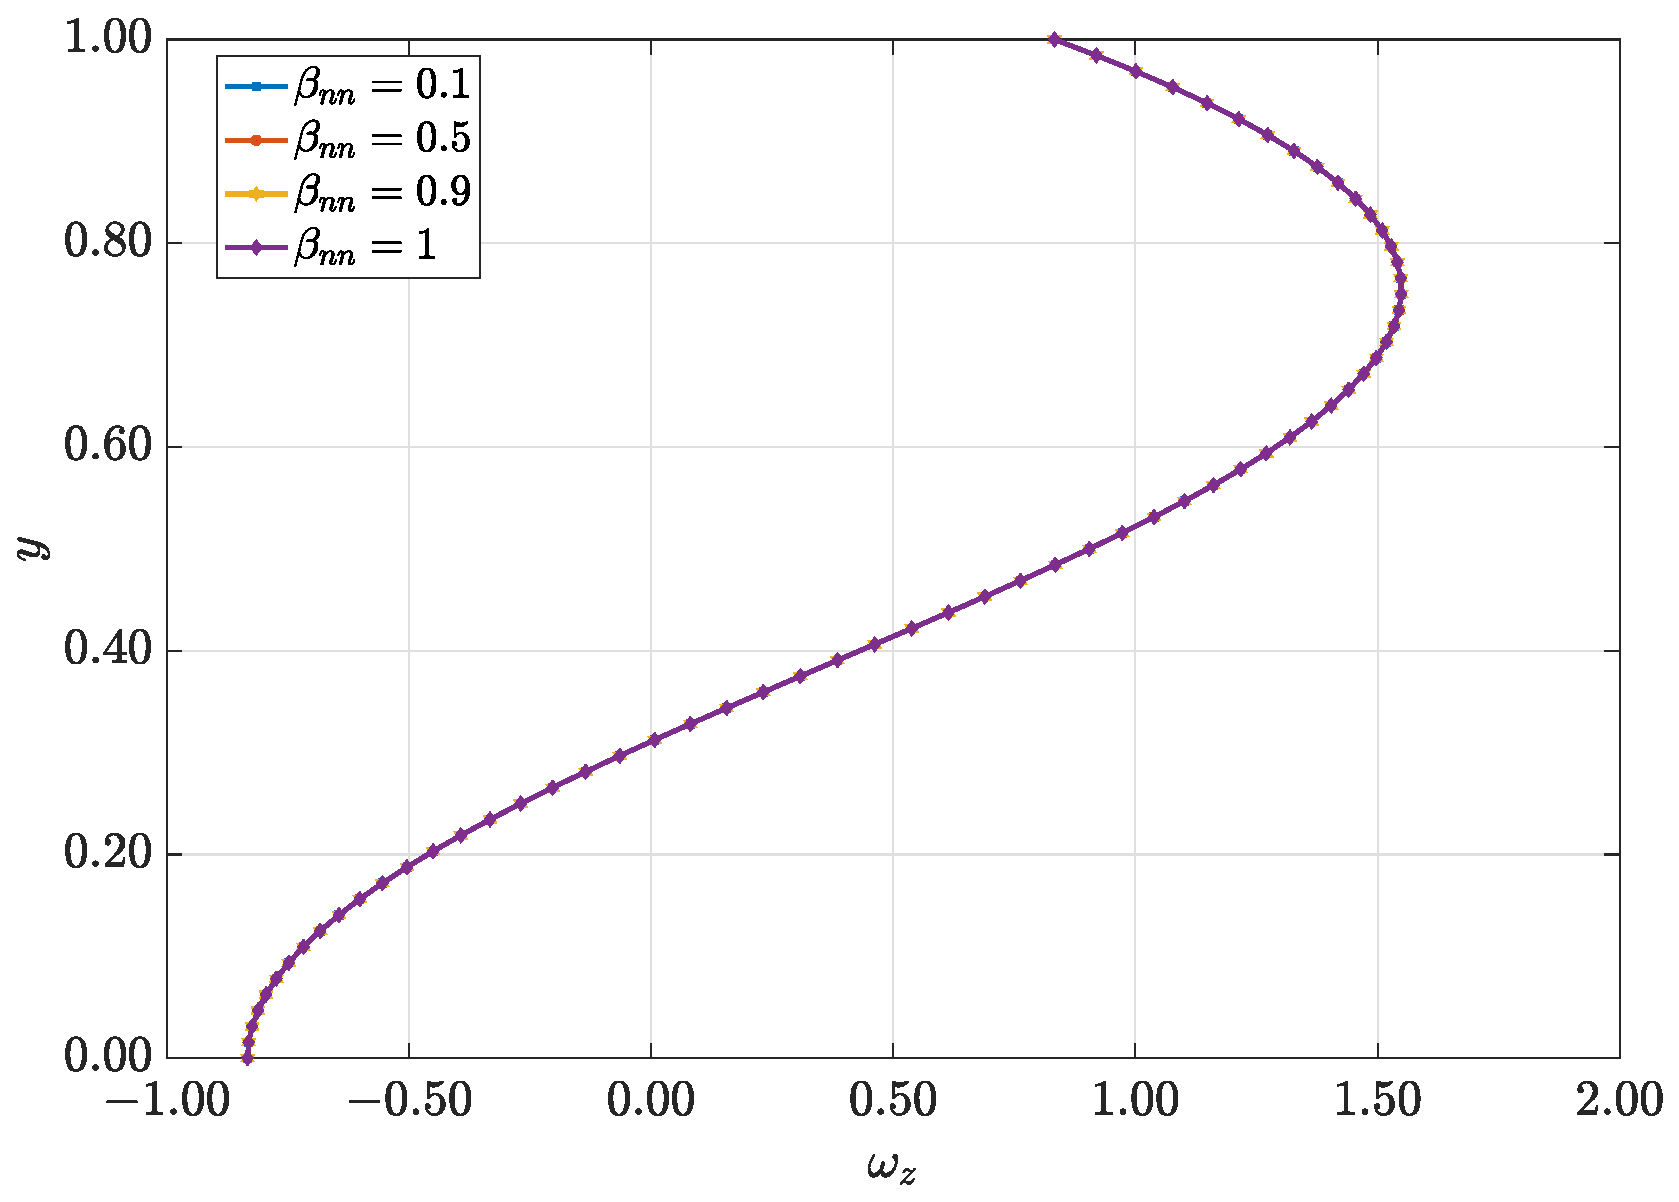
\includegraphics[width=\textwidth]{Slice_x_Tog_Numerical_NormErr_2nd_Betann_1_Re_1000_Wi_1_epsilon_0_xi_0_alphaG_0_Dt_1e-06_at_0.05_tipsim_1_MMS_12_x0.25y0.25_Wz.eps}
        \caption{Profile at $x=0.25$ for the vorticity $(\omega_{z})$}
        \label{fig_slice_x_wz_2nd_Case1_oldroydB}
    \end{subfigure}
    \vspace{0.2cm}
    \qquad
    \begin{subfigure}[b]{.46\textwidth}
        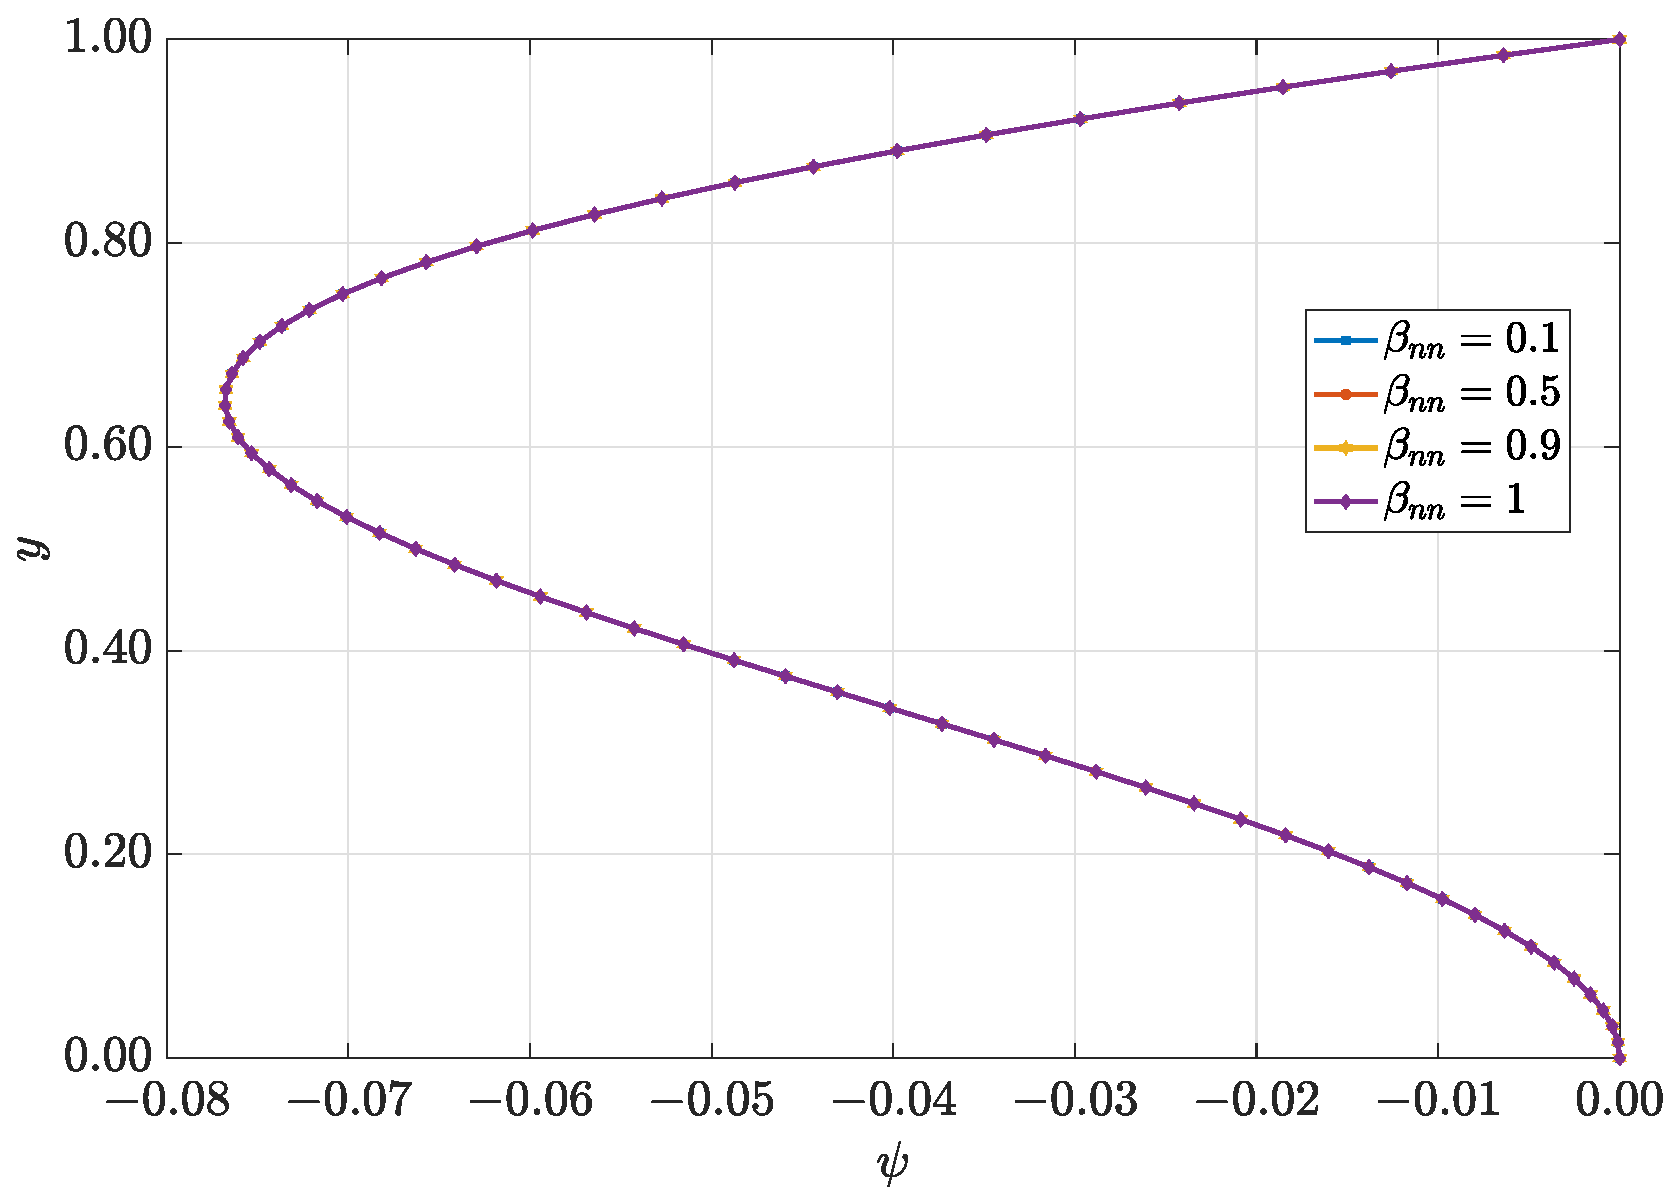
\includegraphics[width=\textwidth]{Slice_x_Tog_Numerical_NormErr_2nd_Betann_1_Re_1000_Wi_1_epsilon_0_xi_0_alphaG_0_Dt_1e-06_at_0.05_tipsim_1_MMS_12_x0.25y0.25_Psi.eps}
        \caption{Profile at $x=0.25$ for the stream function $(\Psi)$}
        \label{fig_slice_x_psi_2nd_Case1_oldorydb}
    \end{subfigure}
    \vspace{0.2cm}
    \caption{Profiles for the velocity field $(u,v)$, vorticity $(\omega_{z})$, and stream function $(\Psi)$, using $\operatorname{Re}=1000$ and $Wi=1$ for the Oldroyd-B viscoelastic fluid flow, where the continuous lines represent the manufactured solutions, and the markers correspond to the numerical solutions, both computed under the same parameters.\label{fig_slice_Solution_uvwzpsi_oldroydb_x}}
\end{figure}

\begin{figure}[H]
    \centering
    \begin{subfigure}[b]{.46\textwidth}
        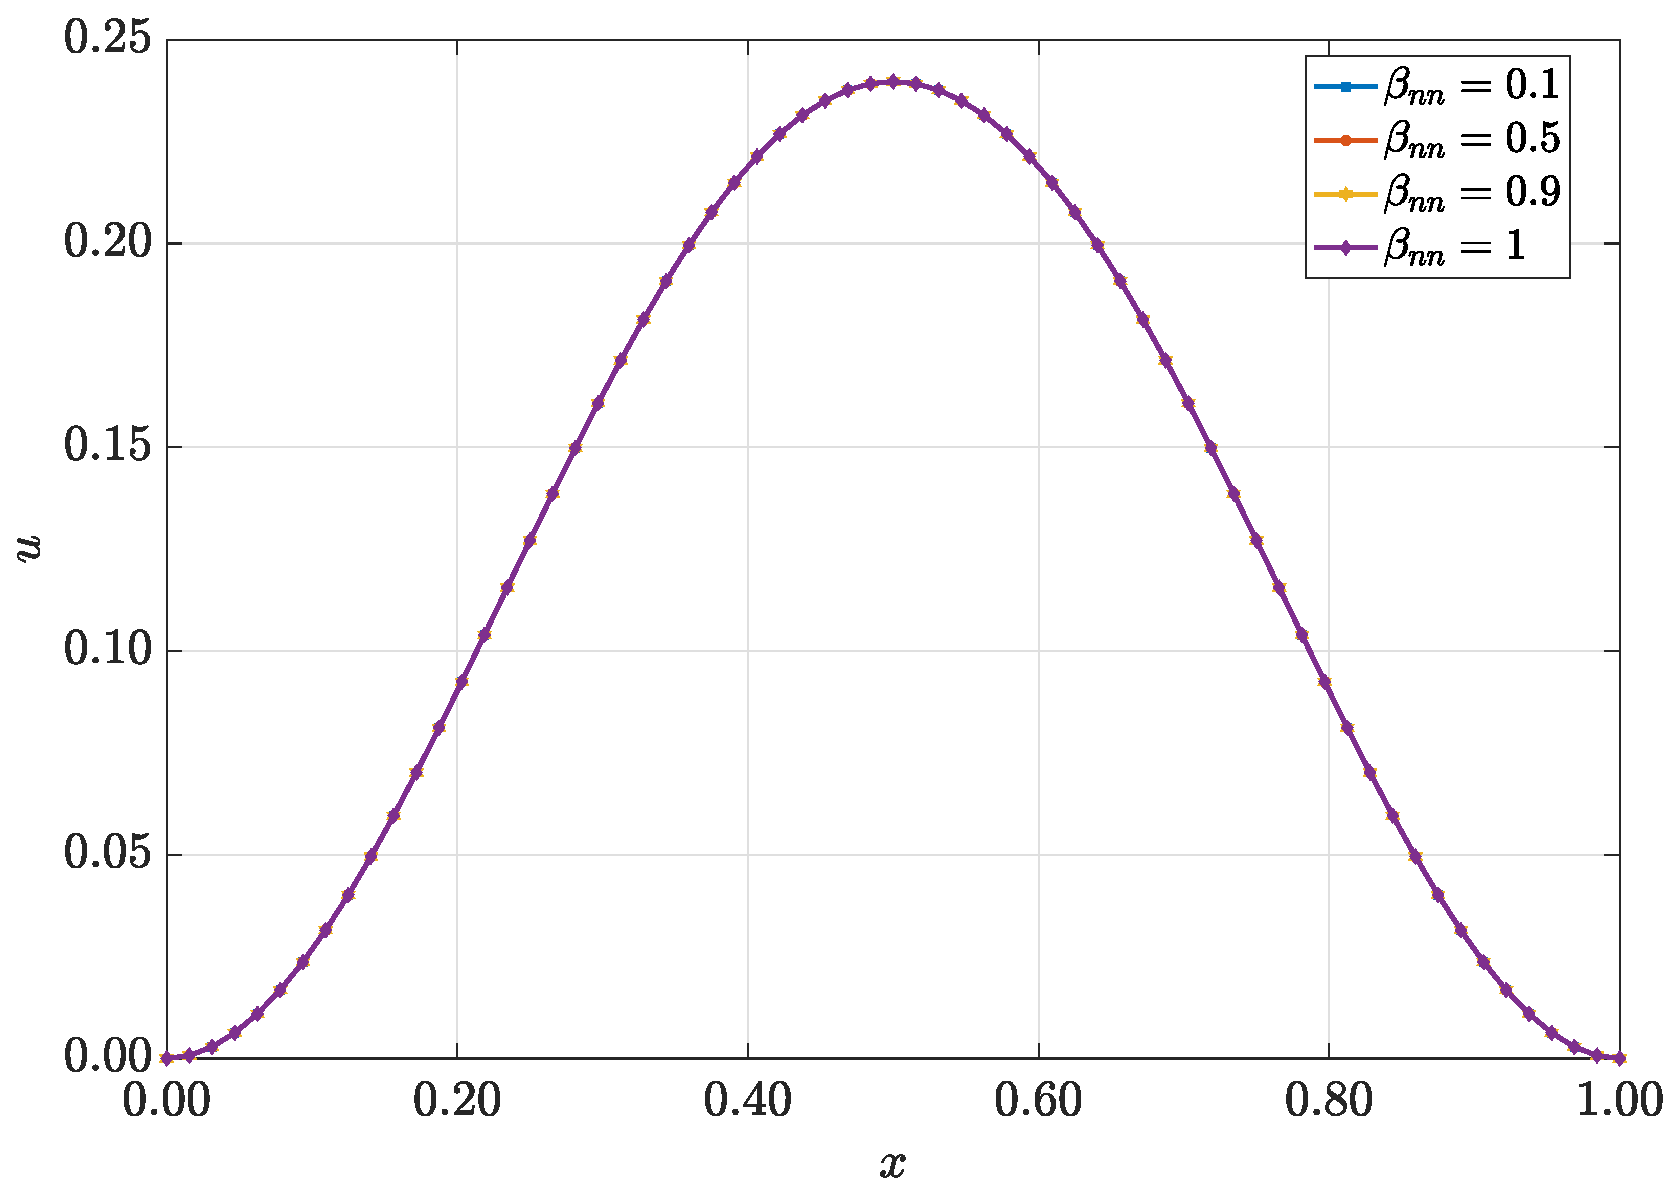
\includegraphics[width=\textwidth]{Slice_y_Tog_Numerical_NormErr_2nd_Betann_1_Re_1000_Wi_1_epsilon_0_xi_0_alphaG_0_Dt_1e-06_at_0.05_tipsim_1_MMS_12_x0.75y0.75_U.eps}
        \caption{Profile at $y=0.75$ for the velocity field component $(u)$}
        \label{fig_slice_y_u_2nd_Case1_oldorydb}
    \end{subfigure}
    \vspace{0.2cm}
    \qquad
    \begin{subfigure}[b]{.46\textwidth}
        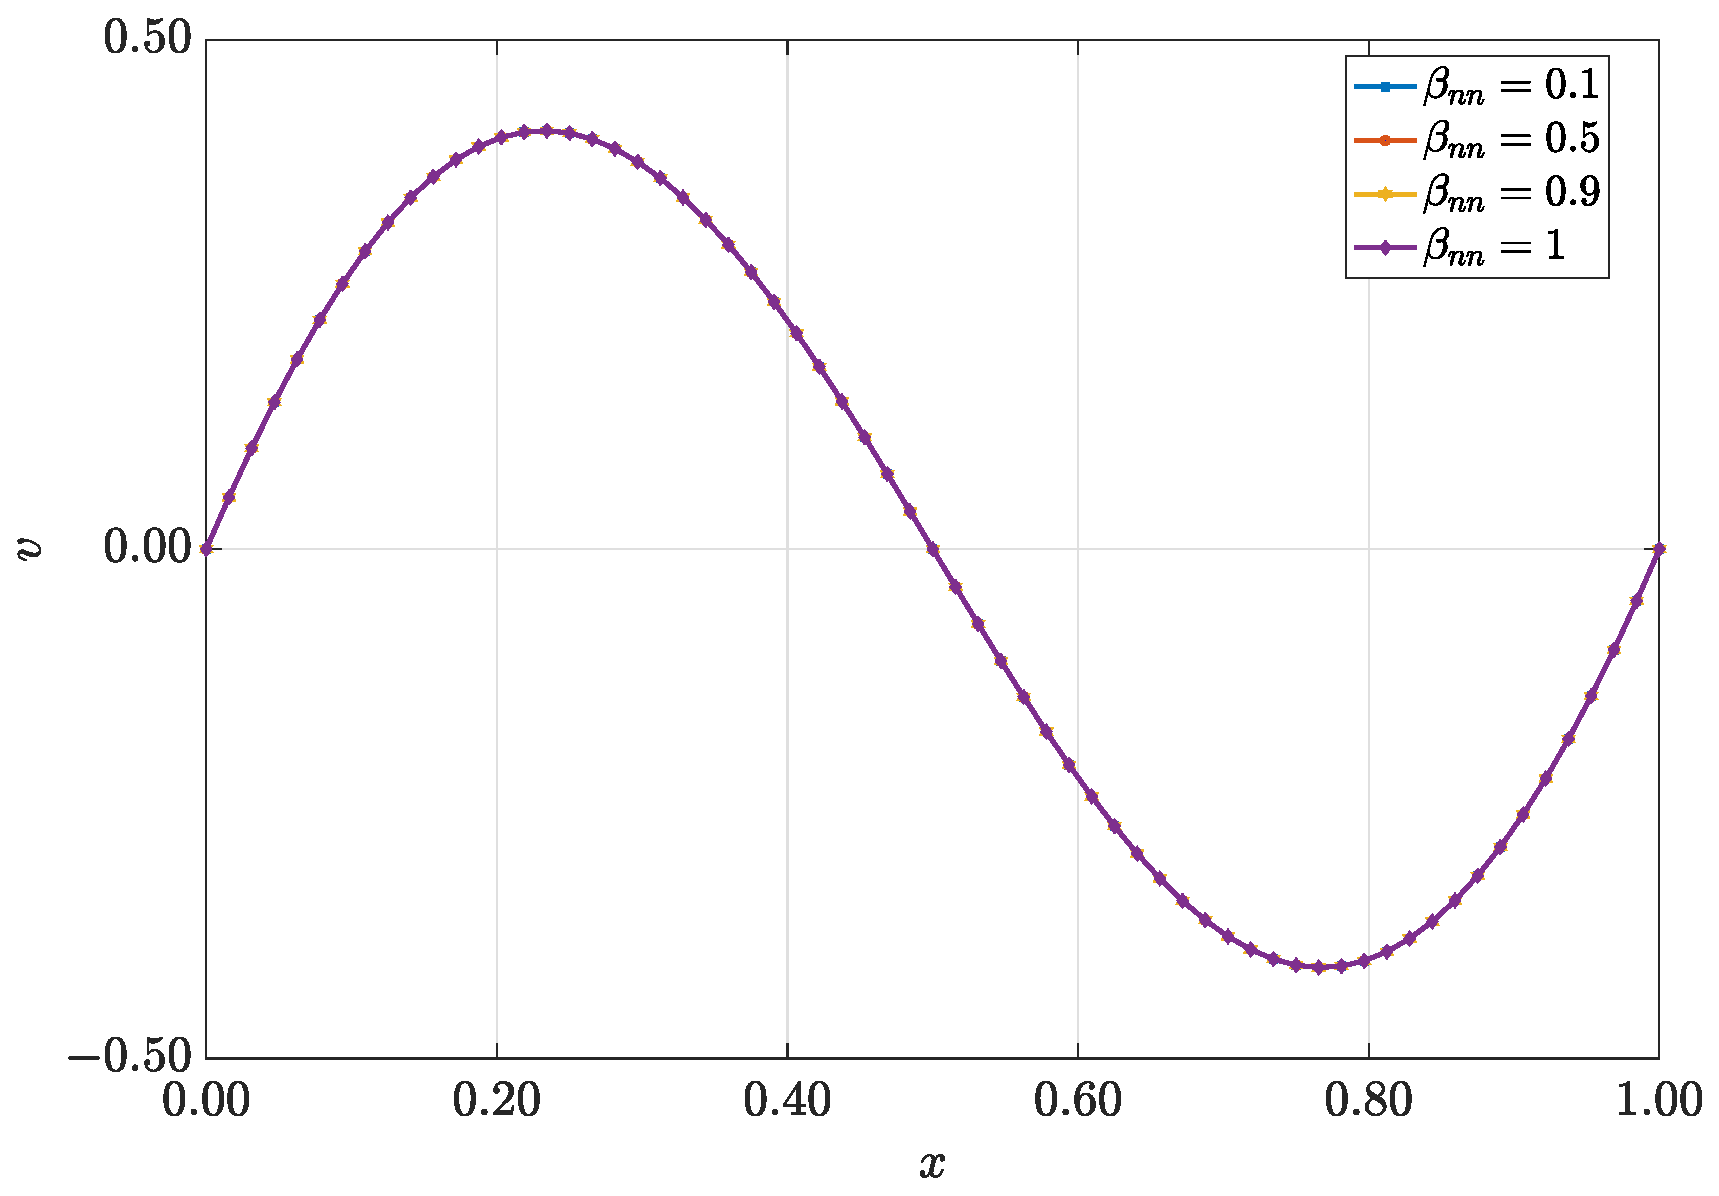
\includegraphics[width=\textwidth]{Slice_y_Tog_Numerical_NormErr_2nd_Betann_1_Re_1000_Wi_1_epsilon_0_xi_0_alphaG_0_Dt_1e-06_at_0.05_tipsim_1_MMS_12_x0.75y0.75_V.eps}
        \caption{Profile at $y=0.75$ for the velocity field component $(v)$}
        \label{fig_slice_y_v_2nd_Case1_oldorydb}
    \end{subfigure}
    \begin{subfigure}[b]{.46\textwidth}
        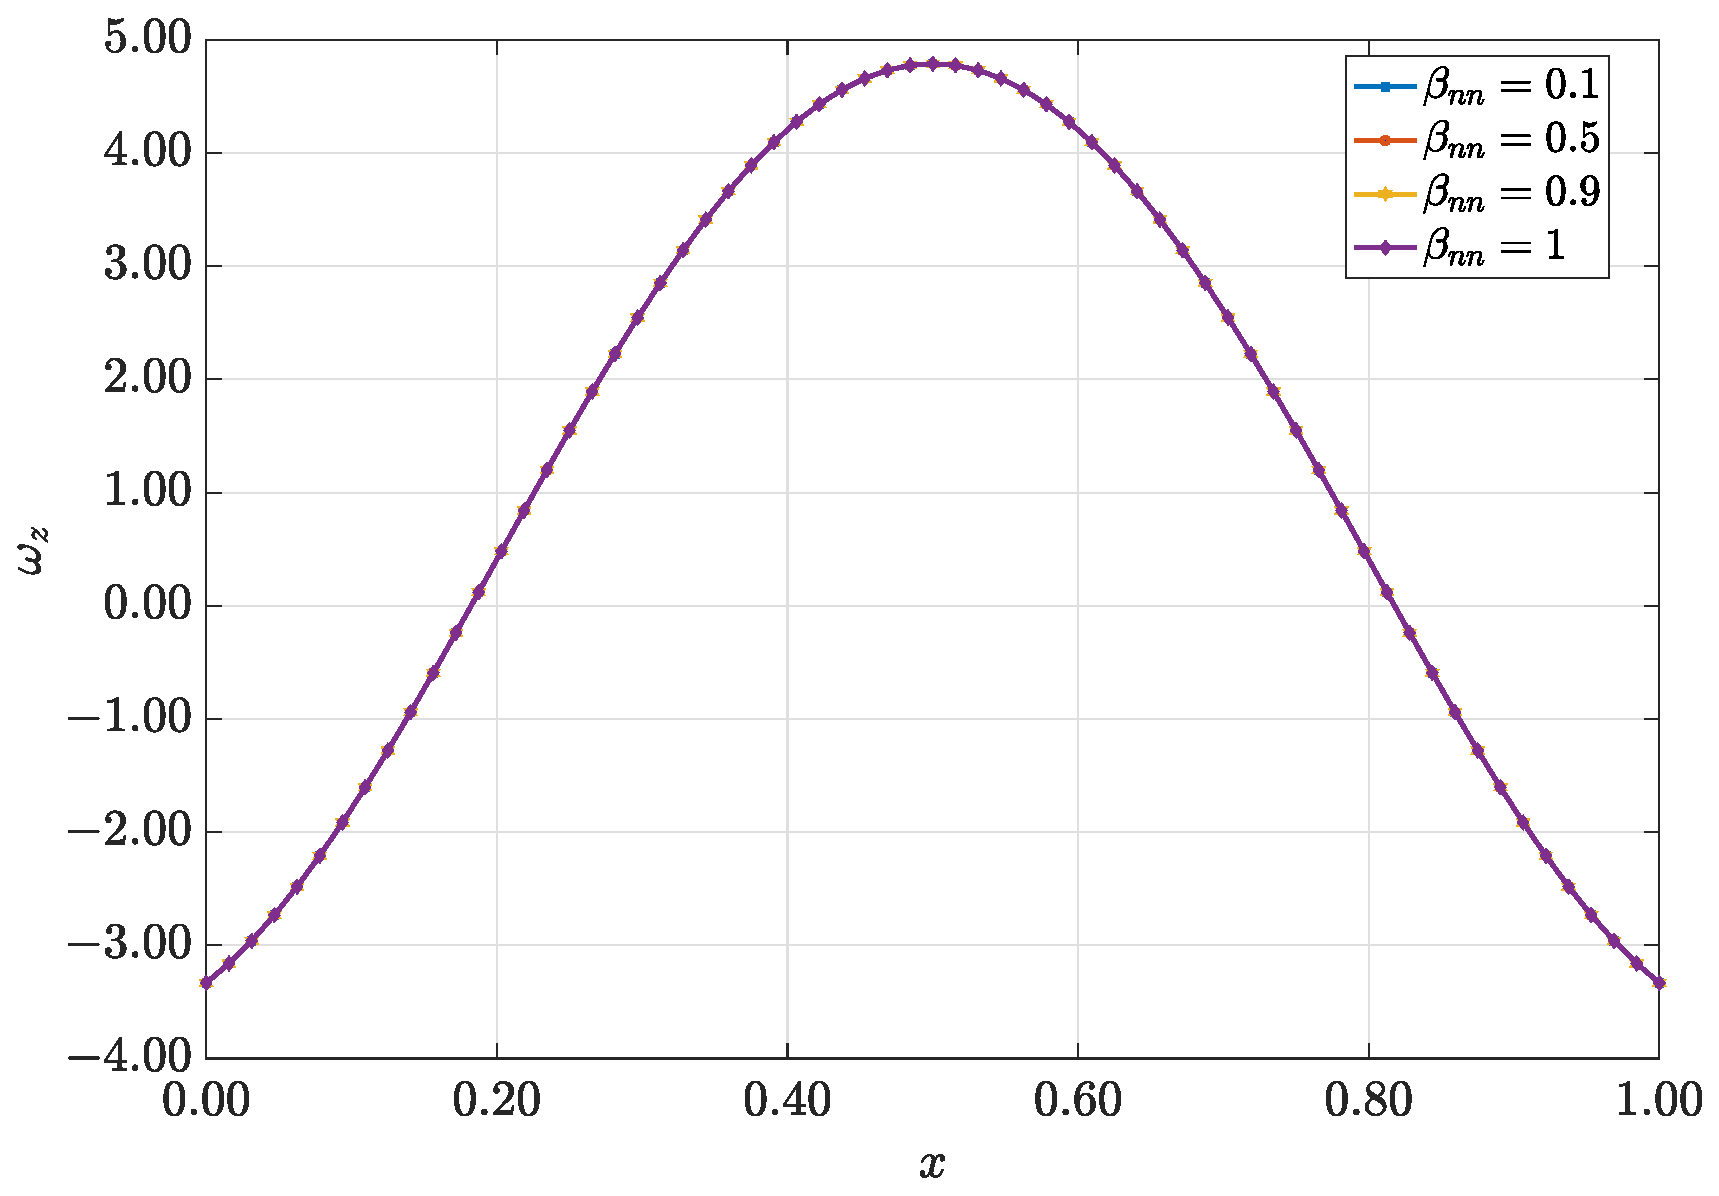
\includegraphics[width=\textwidth]{Slice_y_Tog_Numerical_NormErr_2nd_Betann_1_Re_1000_Wi_1_epsilon_0_xi_0_alphaG_0_Dt_1e-06_at_0.05_tipsim_1_MMS_12_x0.75y0.75_Wz.eps}
        \caption{Profile at $y=0.75$ for the vorticity $(\omega_{z})$}
        \label{fig_slice_y_wz_2nd_Case1_oldorydb}
    \end{subfigure}
    \vspace{0.2cm}
    \qquad
    \begin{subfigure}[b]{.46\textwidth}
        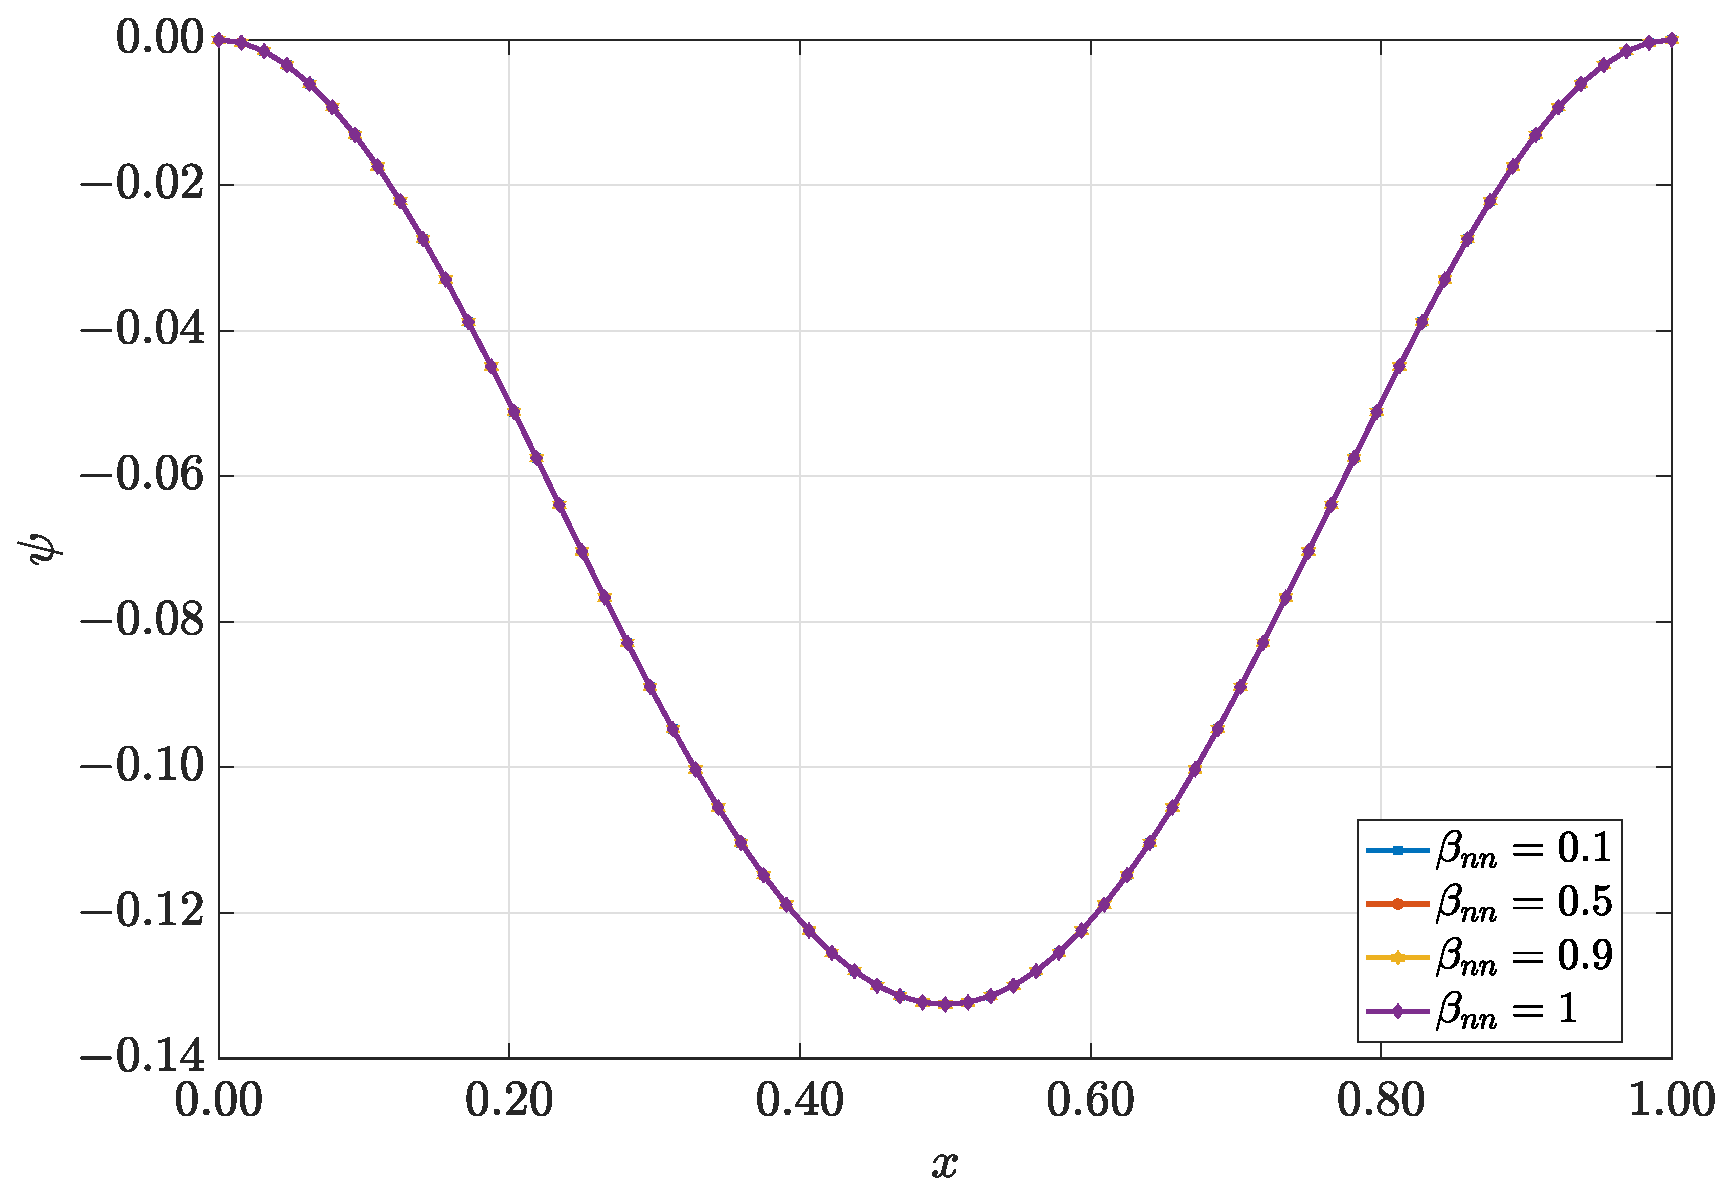
\includegraphics[width=\textwidth]{Slice_y_Tog_Numerical_NormErr_2nd_Betann_1_Re_1000_Wi_1_epsilon_0_xi_0_alphaG_0_Dt_1e-06_at_0.05_tipsim_1_MMS_12_x0.75y0.75_Psi.eps}
        \caption{Profile at $y=0.75$ for the stream function $(\Psi)$}
        \label{fig_slice_y_psi_2nd_Case1_oldorydb}
    \end{subfigure}
    \vspace{0.02cm}
    \caption{Profiles for the velocity field $(u,v)$, vorticity $(\omega_{z})$, and stream function $(\Psi)$, using $\operatorname{Re}=1000$ and $Wi=1$ for the Oldroyd-B viscoelastic fluid flow, where the continuous lines represent the manufactured solutions, and the markers correspond to the numerical solutions, both computed under the same parameters.\label{fig_slice_Solution_uvwzpsi_oldroydb_y}}
\end{figure}

Figures \ref{fig_slice_Solution_TxxTxyTyy_oldroydb_x} and
\ref{fig_slice_Solution_TxxTxyTyy_oldroydb_y} show profiles for the polymeric
tensor components $(T_{xx}, T_{xy}, T_{yy})$, providing insight into the
distribution of normal and shear stresses within the flow domain along the
lines $x=0.25$ and $y=0.75$, respectively, for the Oldroyd-B constitutive model
under conditions $\operatorname{Re}=1000$ and \mbox{$Wi=1$}, where the
continuous lines represent the manufactured solutions, and the markers
correspond to the numerical solutions, both computed under the same parameters.
\begin{figure}[H]
    \centering  
    \begin{subfigure}[b]{.46\textwidth}
        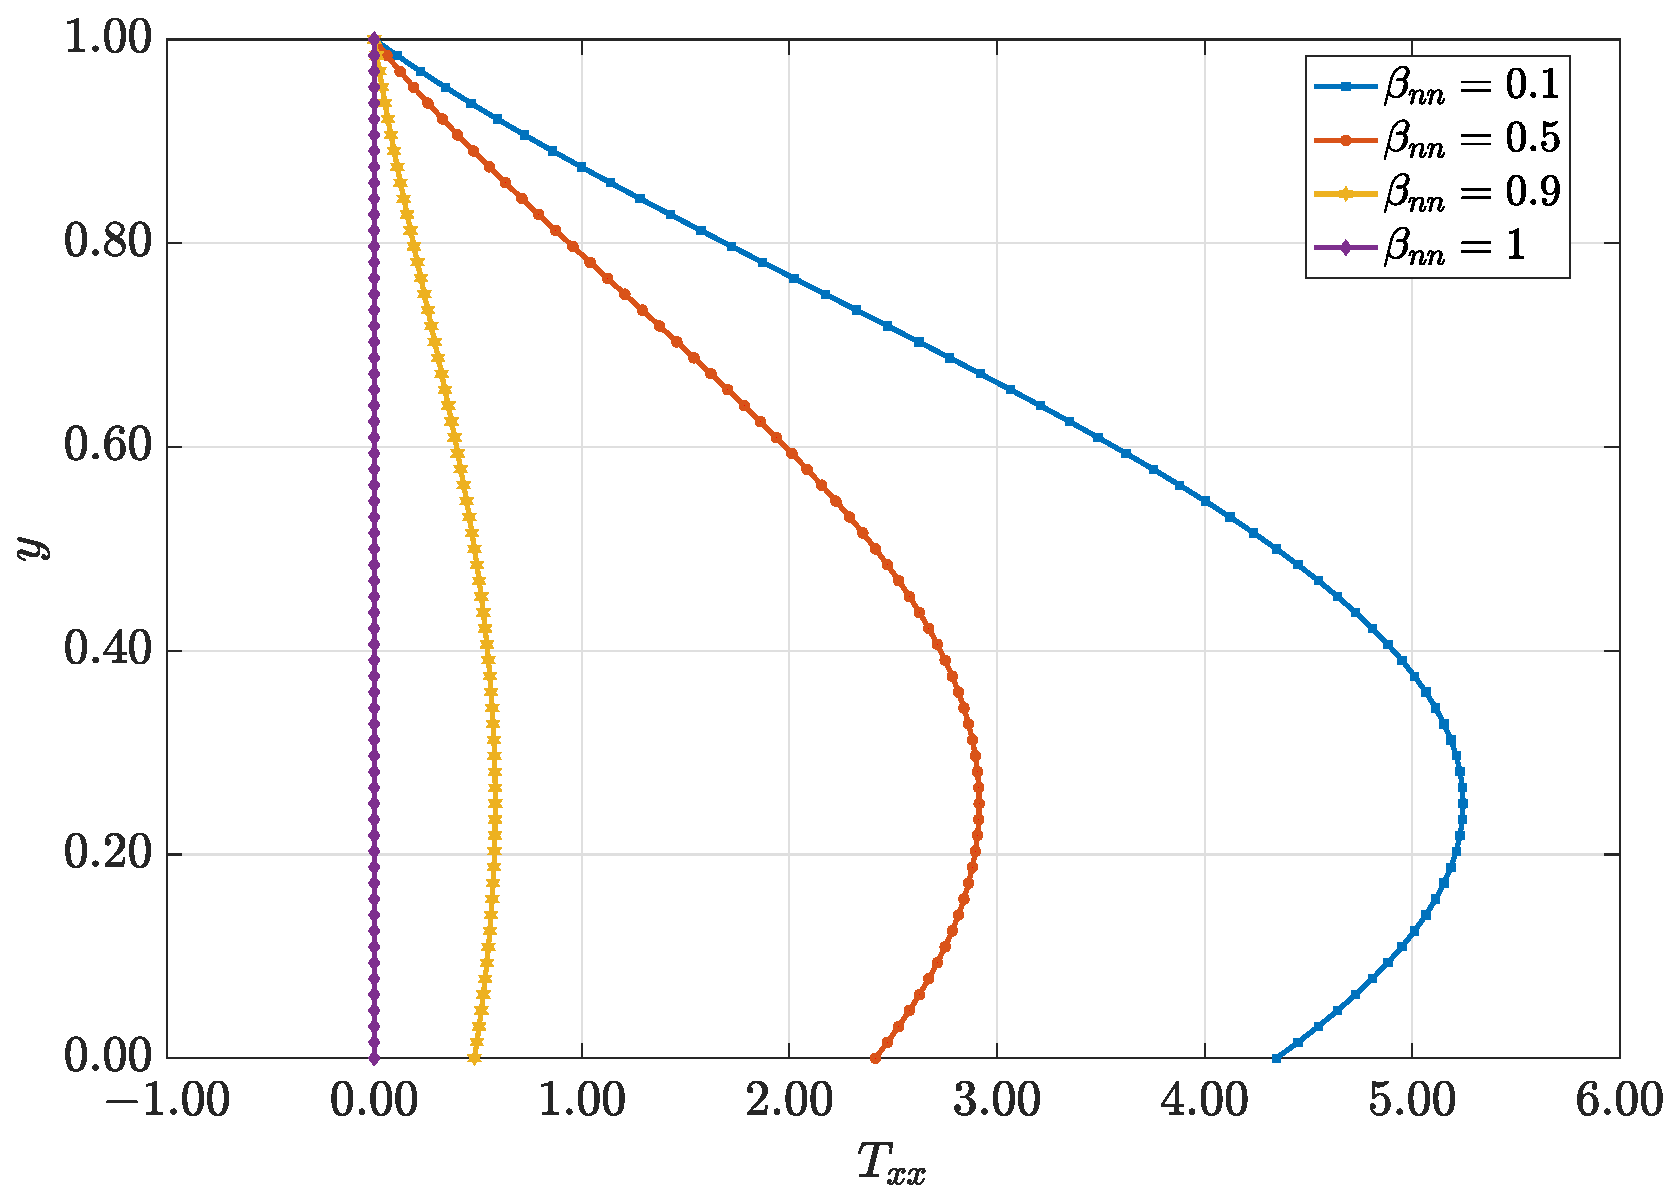
\includegraphics[width=\textwidth]{Slice_x_Tog_Numerical_NormErr_2nd_Betann_1_Re_1000_Wi_1_epsilon_0_xi_0_alphaG_0_Dt_1e-06_at_0.05_tipsim_1_MMS_12_x0.25y0.25_Txx.eps}
        \caption{Profile at $x=0.25$ for the polymeric tensor component $T_{xx}$}
        \label{fig_slice_x_txx_2nd_Case1_oldroydB}
    \end{subfigure}
    \vspace{0.2cm}
    \qquad
    \begin{subfigure}[b]{.46\textwidth}
        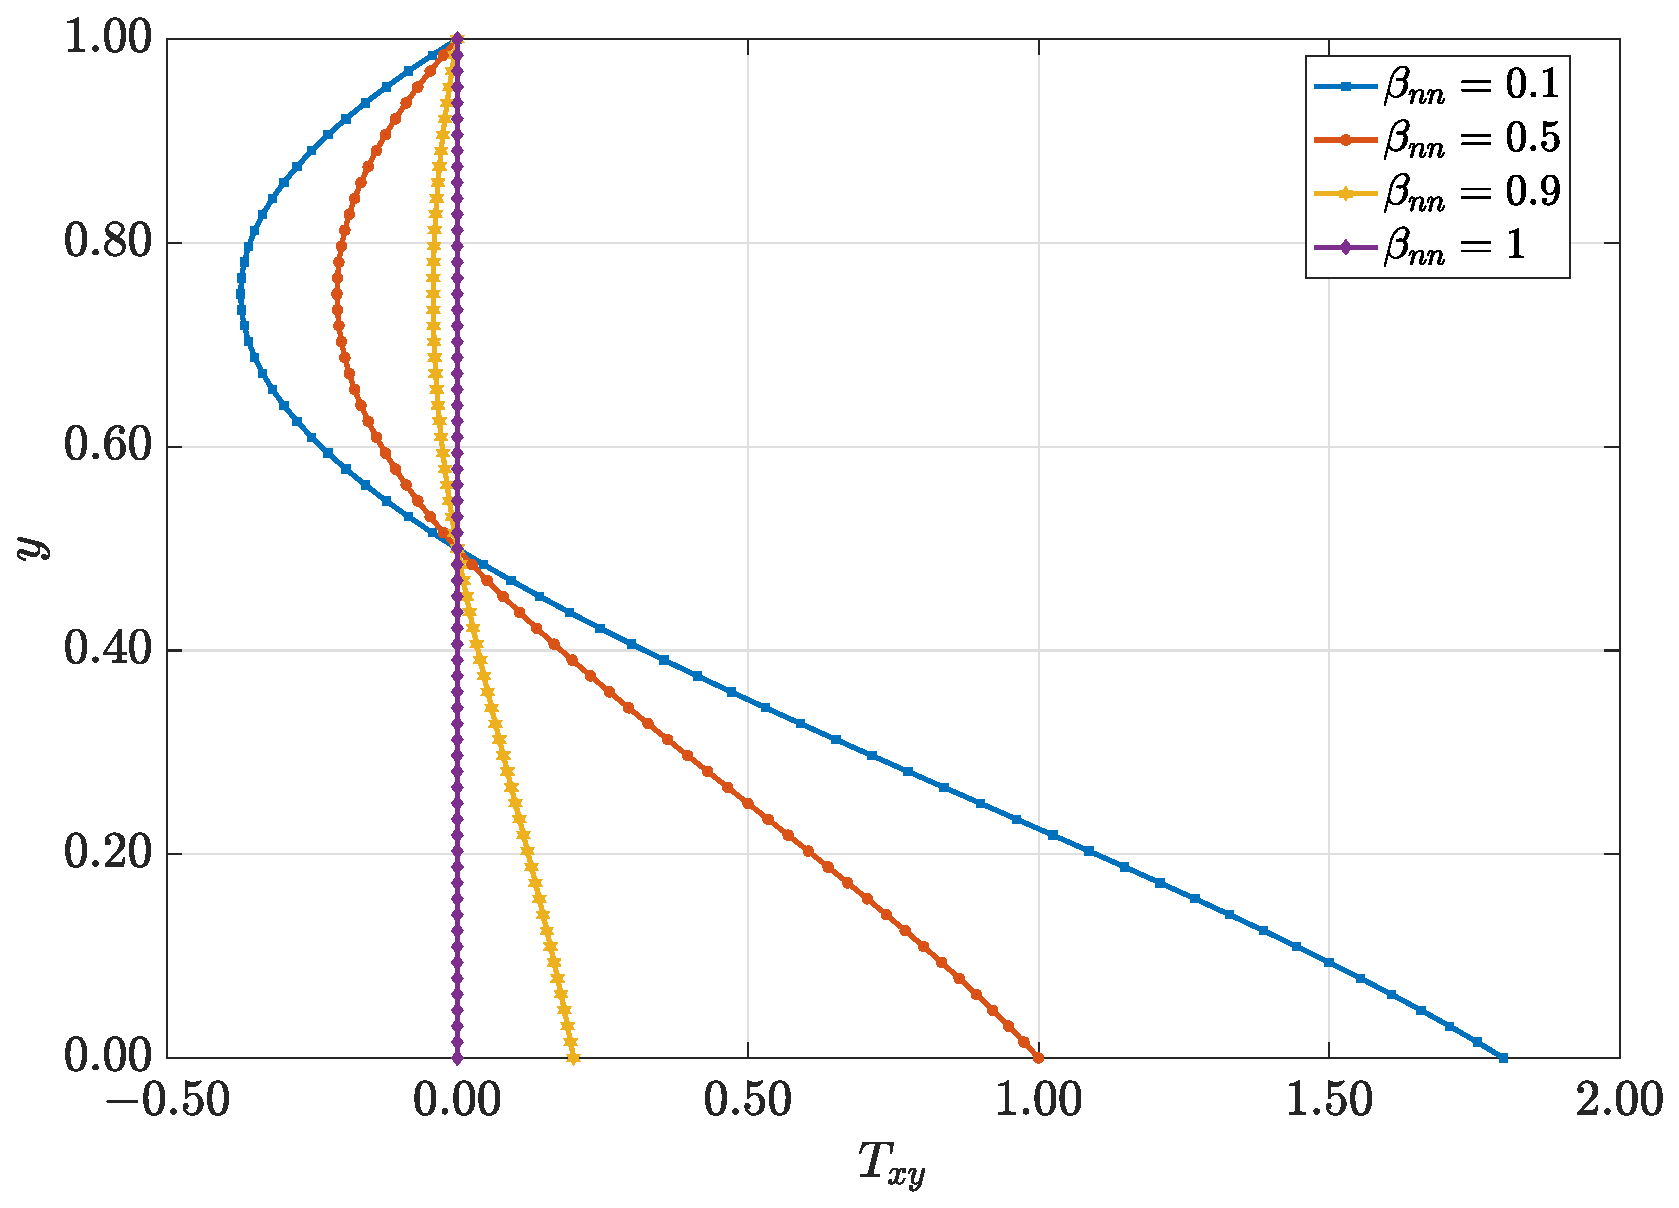
\includegraphics[width=\textwidth]{Slice_x_Tog_Numerical_NormErr_2nd_Betann_1_Re_1000_Wi_1_epsilon_0_xi_0_alphaG_0_Dt_1e-06_at_0.05_tipsim_1_MMS_12_x0.25y0.25_Txy.eps}
        \caption{Profile at $x=0.25$ for the polymeric tensor component $T_{xy}$}
        \label{fig_slice_x_txy_2nd_Case1_oldorydb}
    \end{subfigure}
    \begin{subfigure}[b]{.46\textwidth}
        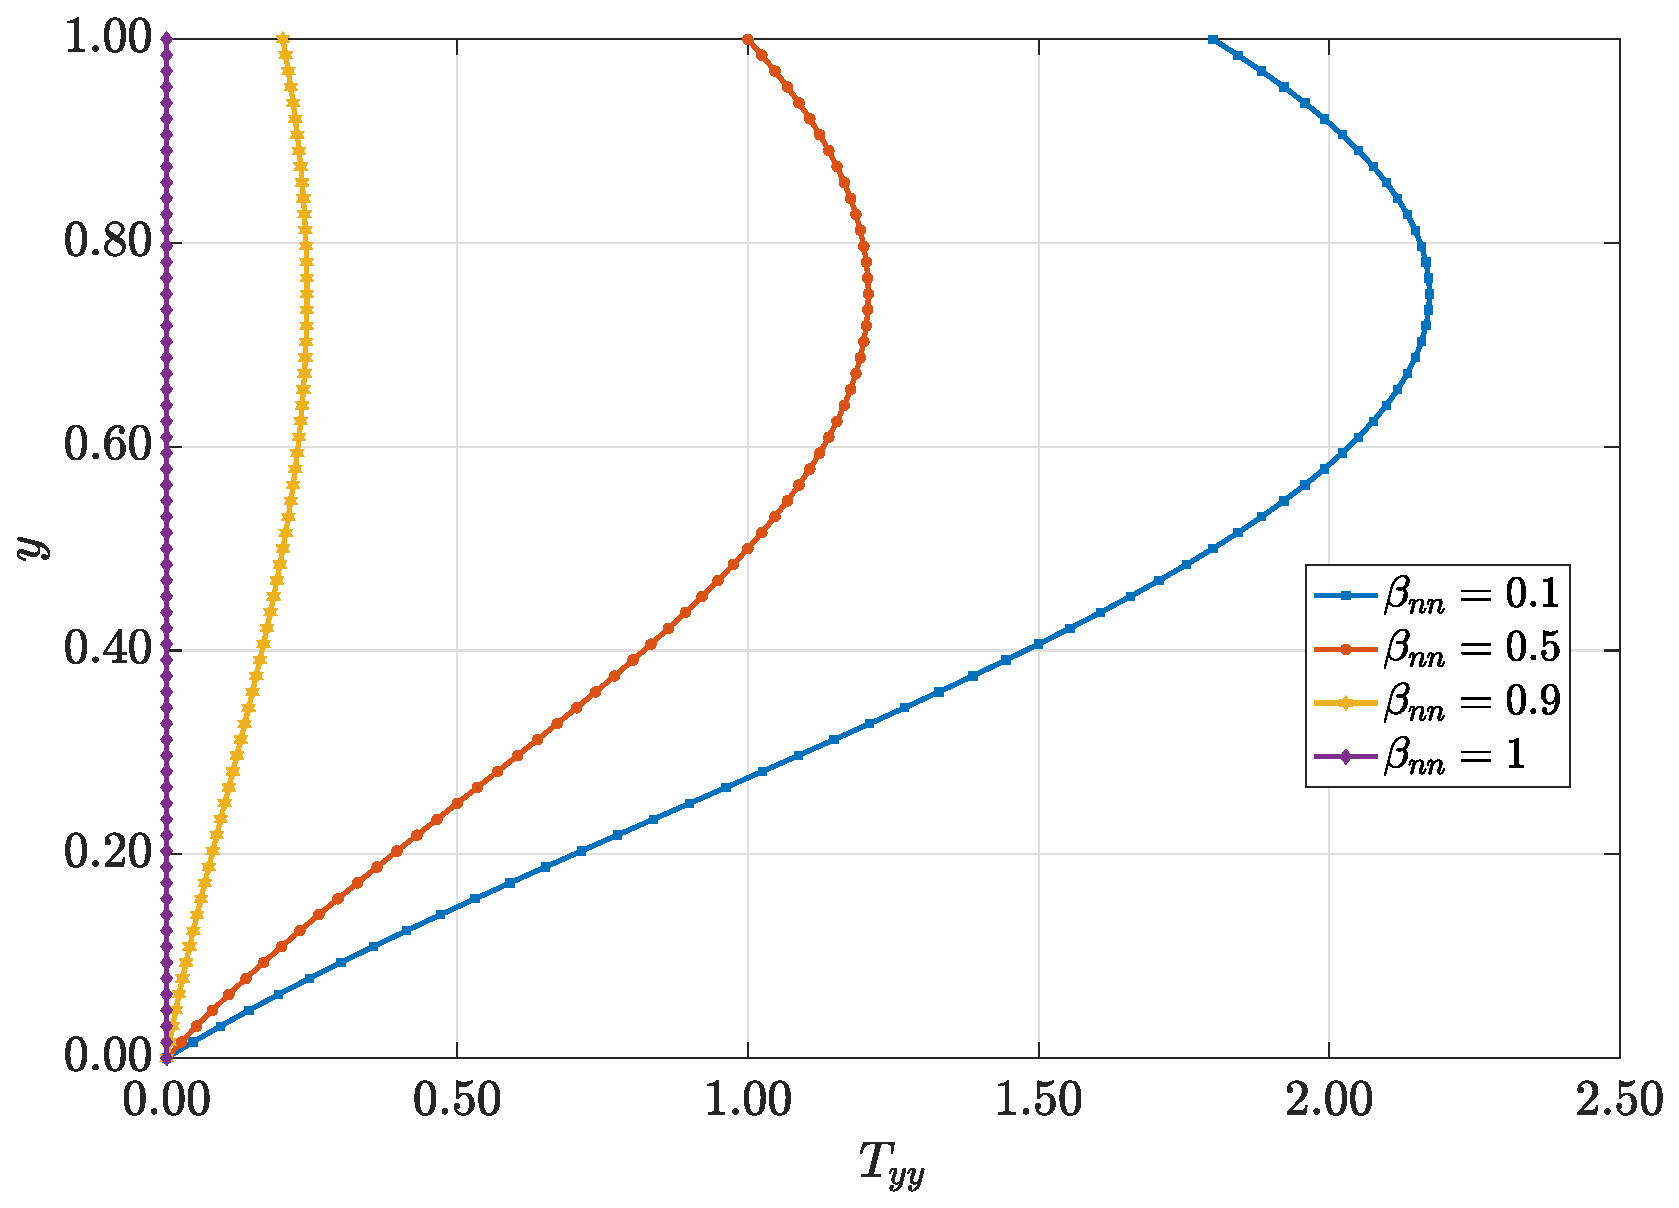
\includegraphics[width=\textwidth]{Slice_x_Tog_Numerical_NormErr_2nd_Betann_1_Re_1000_Wi_1_epsilon_0_xi_0_alphaG_0_Dt_1e-06_at_0.05_tipsim_1_MMS_12_x0.25y0.25_Tyy.eps}
        \caption{Profile at $x=0.25$ for the polymeric tensor component $T_{yy}$}
        \label{fig_slice_x_tyy_2nd_Case1_oldroydB}
    \end{subfigure}
    \vspace{0.02cm}
    \caption{Profiles for the polymeric tensor components ($T_{xx}, T_{xy}, T_{yy}$) at $x=0.25$, with $\operatorname{Re}=1000$ and $Wi=1$ for the Oldroyd-B viscoelastic fluid flow, where the continuous lines represent the manufactured solutions, and the markers correspond to the numerical solutions, both computed under the same parameters.\label{fig_slice_Solution_TxxTxyTyy_oldroydb_x}}
\end{figure}

\begin{figure}[H]
    \centering  
    \begin{subfigure}[b]{.46\textwidth}
        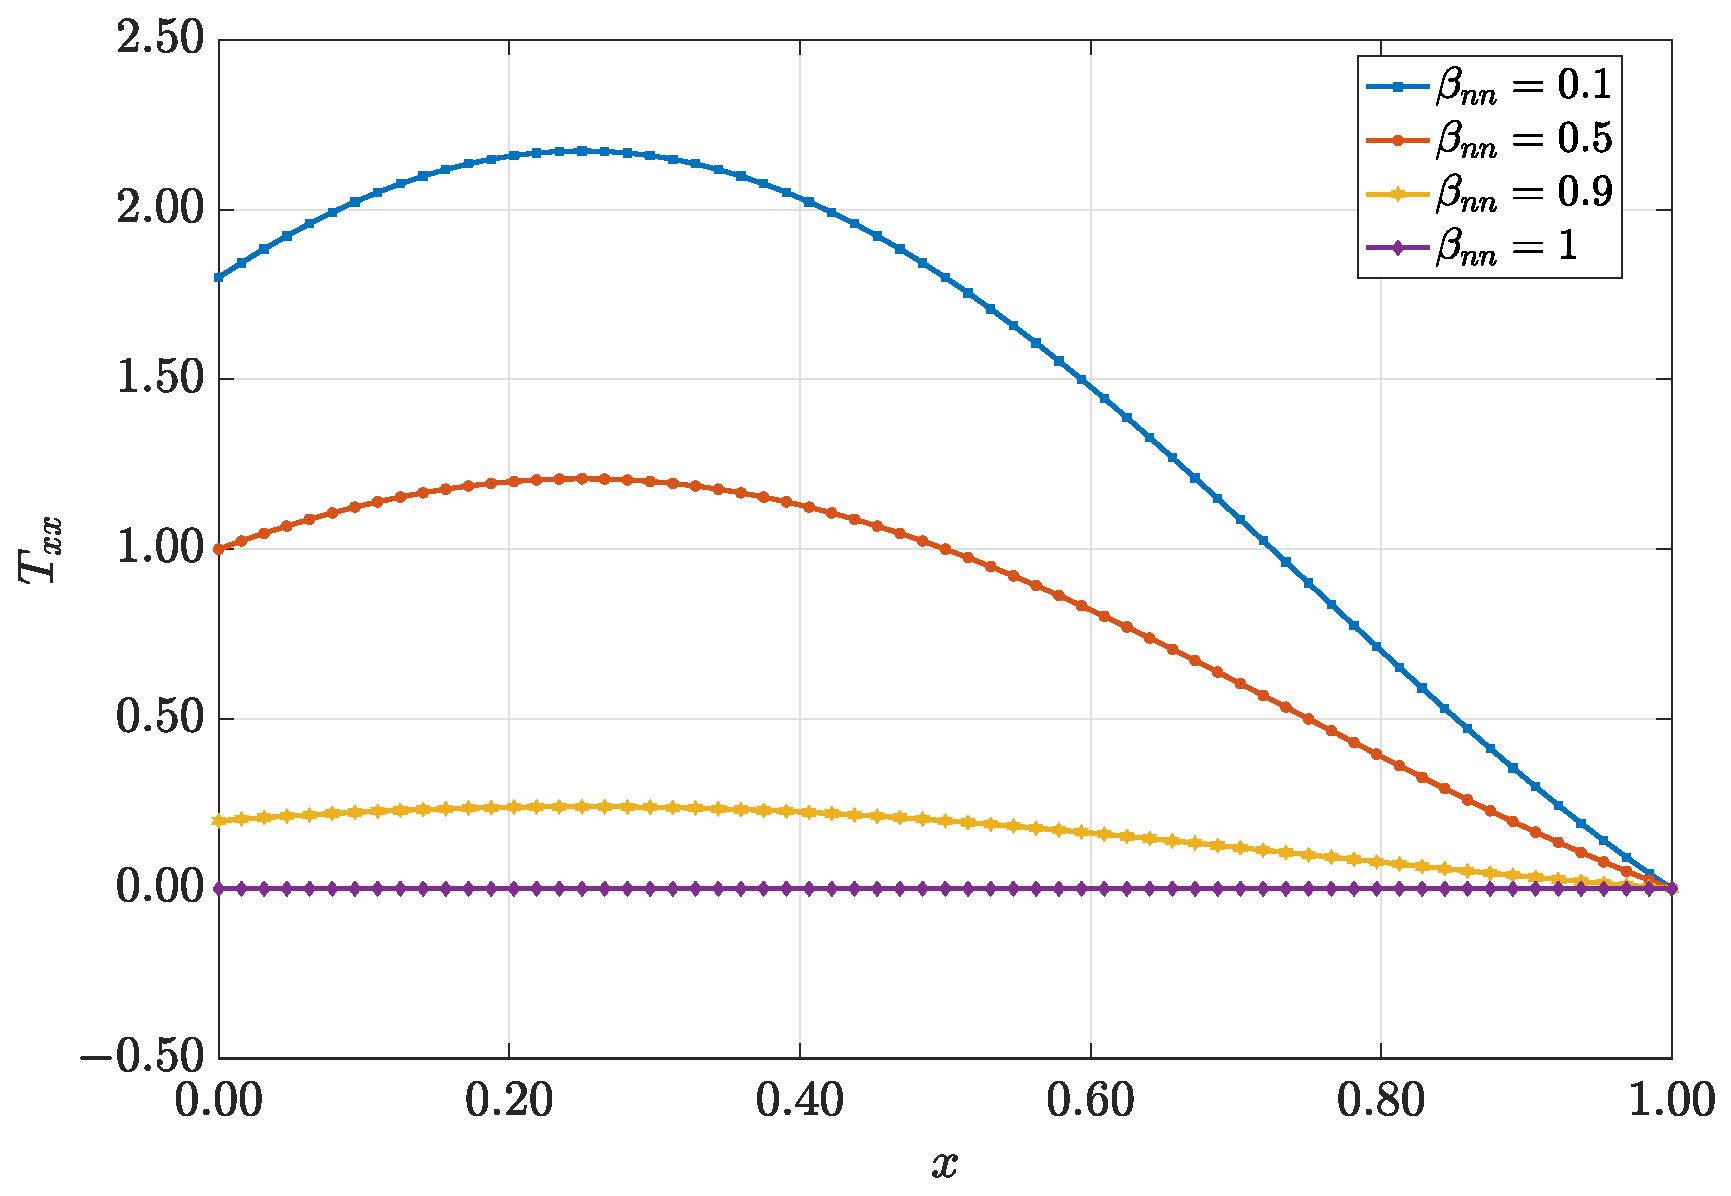
\includegraphics[width=\textwidth]{Slice_y_Tog_Numerical_NormErr_2nd_Betann_1_Re_1000_Wi_1_epsilon_0_xi_0_alphaG_0_Dt_1e-06_at_0.05_tipsim_1_MMS_12_x0.75y0.75_Txx.eps}
        \caption{Profile at $y=0.75$ for the polymeric tensor component $T_{xx}$}
        \label{fig_slice_y_txx_2nd_Case1_oldorydb}
    \end{subfigure}
    \vspace{0.2cm}
    \qquad
    \begin{subfigure}[b]{.46\textwidth}
        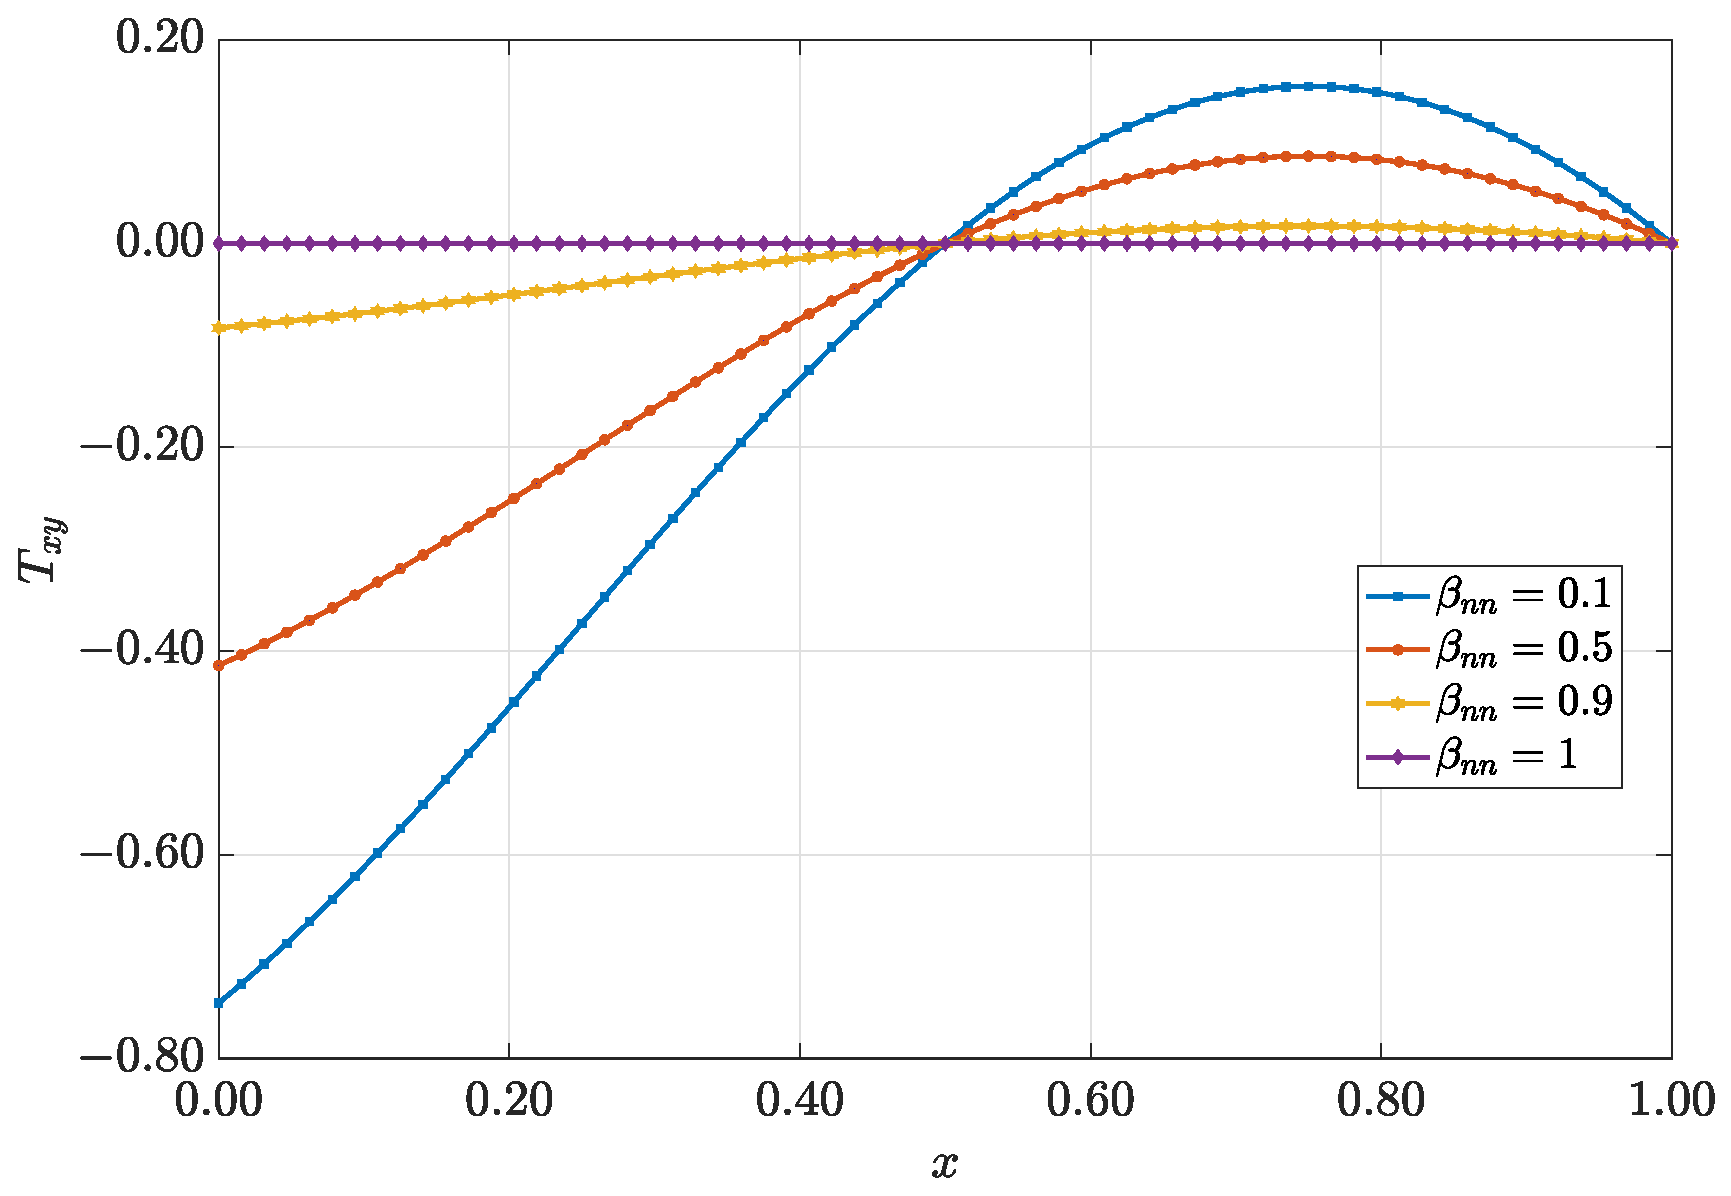
\includegraphics[width=\textwidth]{Slice_y_Tog_Numerical_NormErr_2nd_Betann_1_Re_1000_Wi_1_epsilon_0_xi_0_alphaG_0_Dt_1e-06_at_0.05_tipsim_1_MMS_12_x0.75y0.75_Txy.eps}
        \caption{Profile at $y=0.75$ for the polymeric tensor component $T_{xy}$}
        \label{fig_slice_y_txy_2nd_Case1_oldorydb}
    \end{subfigure}
    \begin{subfigure}[b]{.46\textwidth}
        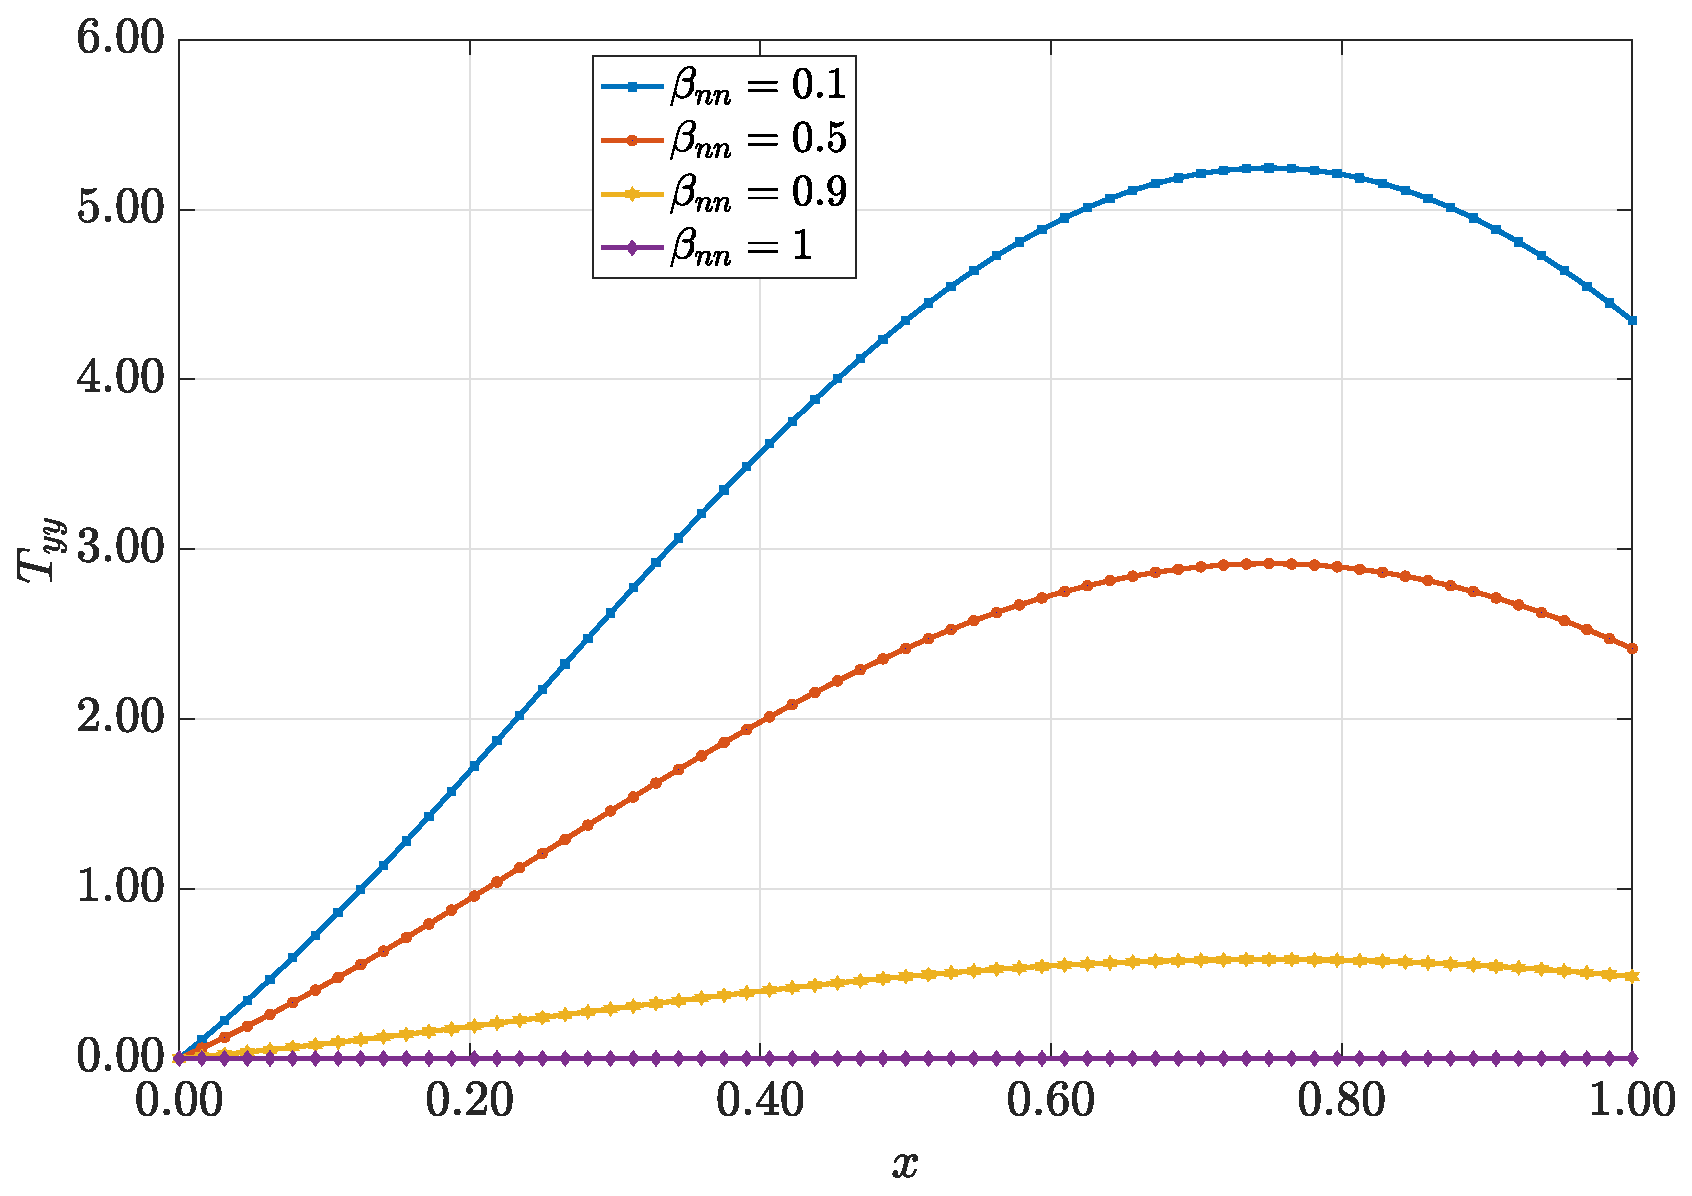
\includegraphics[width=\textwidth]{Slice_y_Tog_Numerical_NormErr_2nd_Betann_1_Re_1000_Wi_1_epsilon_0_xi_0_alphaG_0_Dt_1e-06_at_0.05_tipsim_1_MMS_12_x0.75y0.75_Tyy.eps}
        \caption{Profile at $y=0.75$ for the polymeric tensor component $T_{yy}$}
        \label{fig_slice_y_tyy_2nd_Case1_oldorydb}
    \end{subfigure}
    \vspace{0.02cm}
    \caption{Profiles for the polymeric tensor components ($T_{xx}, T_{xy}, T_{yy}$) at $y=0.75$, with $\operatorname{Re}=1000$ and $Wi=1$ for the Oldroyd-B viscoelastic fluid flow, where the continuous lines represent the manufactured solutions, and the markers correspond to the numerical solutions, both computed under the same parameters.\label{fig_slice_Solution_TxxTxyTyy_oldroydb_y}}
\end{figure}

In
Figures~\ref{fig_slice_Solution_uvwzpsi_oldroydb_x},~\ref{fig_slice_Solution_uvwzpsi_oldroydb_y},~\ref{fig_slice_Solution_TxxTxyTyy_oldroydb_x}
and~\ref{fig_slice_Solution_TxxTxyTyy_oldroydb_y}, the numerical results align
with the manufactured solutions, showing no discrepancies, which confirms that
the numerical solutions follow the expected behaviour. This consistency not
only highlights the accuracy of the numerical method employed but also
underscores its robustness in reproducing the solutions. In addition, Figures
\ref{fig_slice_Solution_TxxTxyTyy_oldroydb_x} and
\ref{fig_slice_Solution_TxxTxyTyy_oldroydb_y} illustrate that, as the parameter
$\beta_{nn}$ approaches 1, both the manufactured and numerical solutions along
these profiles ($x=0.25$ and $y=0.75$) demonstrate that the polymeric tensor
components $(T_{xx}, T_{xy}, T_{yy})$ tend toward the null tensor. This
reflects a substantial reduction in viscoelastic effects as the fluid behaviour
transitions to that of a Newtonian fluid. In this Newtonian regime, the
polymeric tensor components become negligible, indicating that the flow
dynamics is primarily governed by viscous forces, which is characteristic of
Newtonian fluids.

\subsection{Verification case using the Giesekus constitutive model}
\label{subsec_giesekus}

In simulations using the Giesekus constitutive model, Reynolds numbers ranging
from $\operatorname{Re} = 1,\ 10,\ 100,\ 400$ to $1000$ were used, with a fixed
Weissenberg number of $Wi = 1$ and various solvent viscosity ratios $\beta_{nn}
= 0.1,\ 0.5,\ 0.9$, and $1.0$. Furthermore, the shear-thinning parameter
$\alpha_G$ was set to values of 0.1 and 0.5 to analyse the behaviour of the
constitutive model under different flow regimes. An error analysis was
performed to assess the performance of the method concerning the velocity
field, vorticity, stream function, and polymeric tensor components.

In Figure~\ref{fig_Giesekus_error011}, the error plots for the velocity field
components ($u,~v$) vorticity ($w_z$) and the stream function ($\Psi$) using
different grid sizes ($\Delta x, \Delta y$) are presented for the Giesekus
constitutive model with $\operatorname{Re} = 100$, $Wi = 1$ and $\alpha_G =
0.1$. As shown, the errors consistently decrease as the grid size is reduced.
The convergence order approaches $4.5$, which is expected for high-order
numerical methods. This consistent behaviour reinforces the robustness and
accuracy of the numerical scheme, demonstrating its effectiveness in capturing
the dynamics of non-linear viscoelastic fluids for different solvent viscosity
ratios. This analysis is crucial to validate the model’s ability to correctly
simulate different flow properties.

\begin{figure}[H]
    \centering  
    \begin{subfigure}[b]{.46\textwidth}
        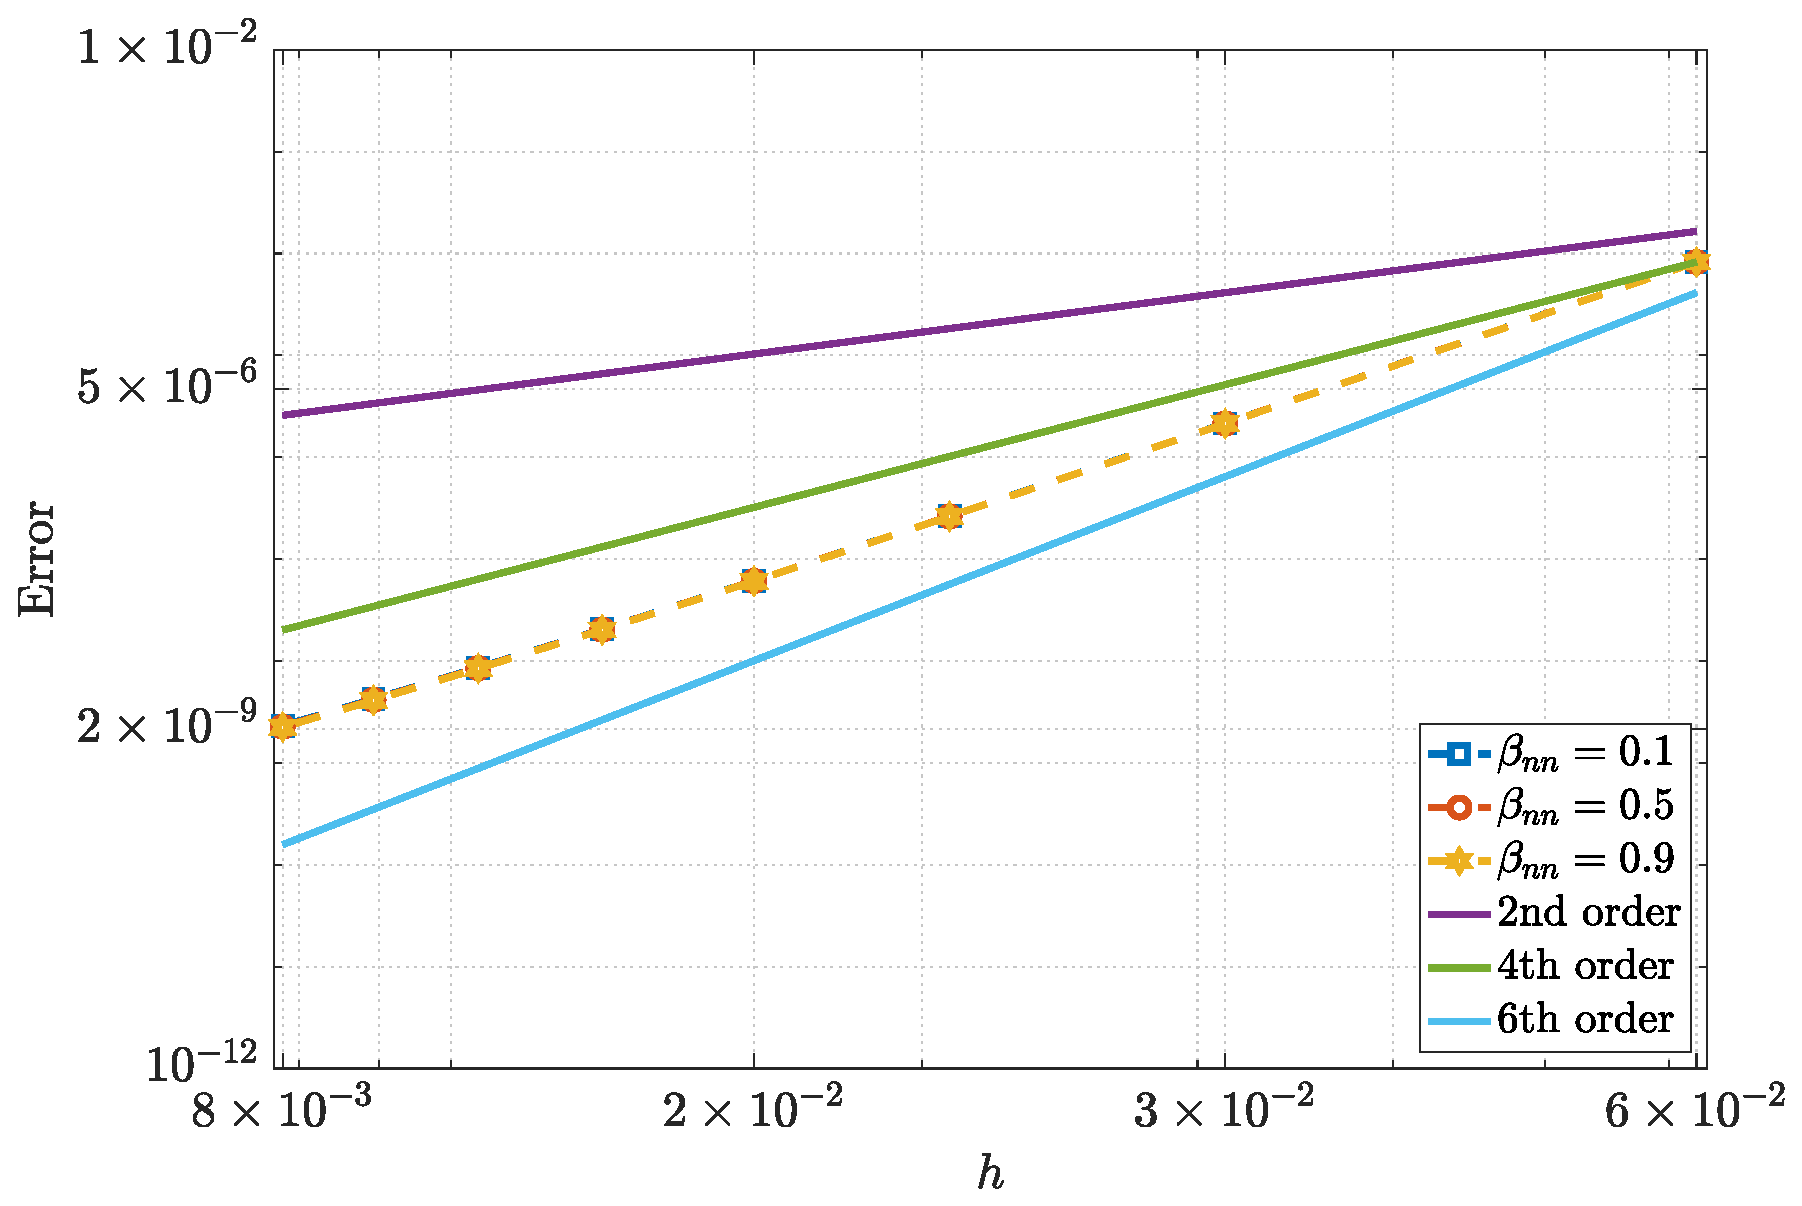
\includegraphics[width=\textwidth]{NormErr_2nd_Re_100_Wi_1_epsilon_0_xi_0_alphaG_0.1_Dt_1e-06_at_0.05_tipsim_1_MMS_12_U.eps}
        \caption{$||u - \overline{u}||_{2}$}
        \label{error_u_2nd_Case1_giesekus_alphaG_0.1}
    \end{subfigure}
    \vspace{0.2cm}
    \qquad
    \begin{subfigure}[b]{.46\textwidth}
        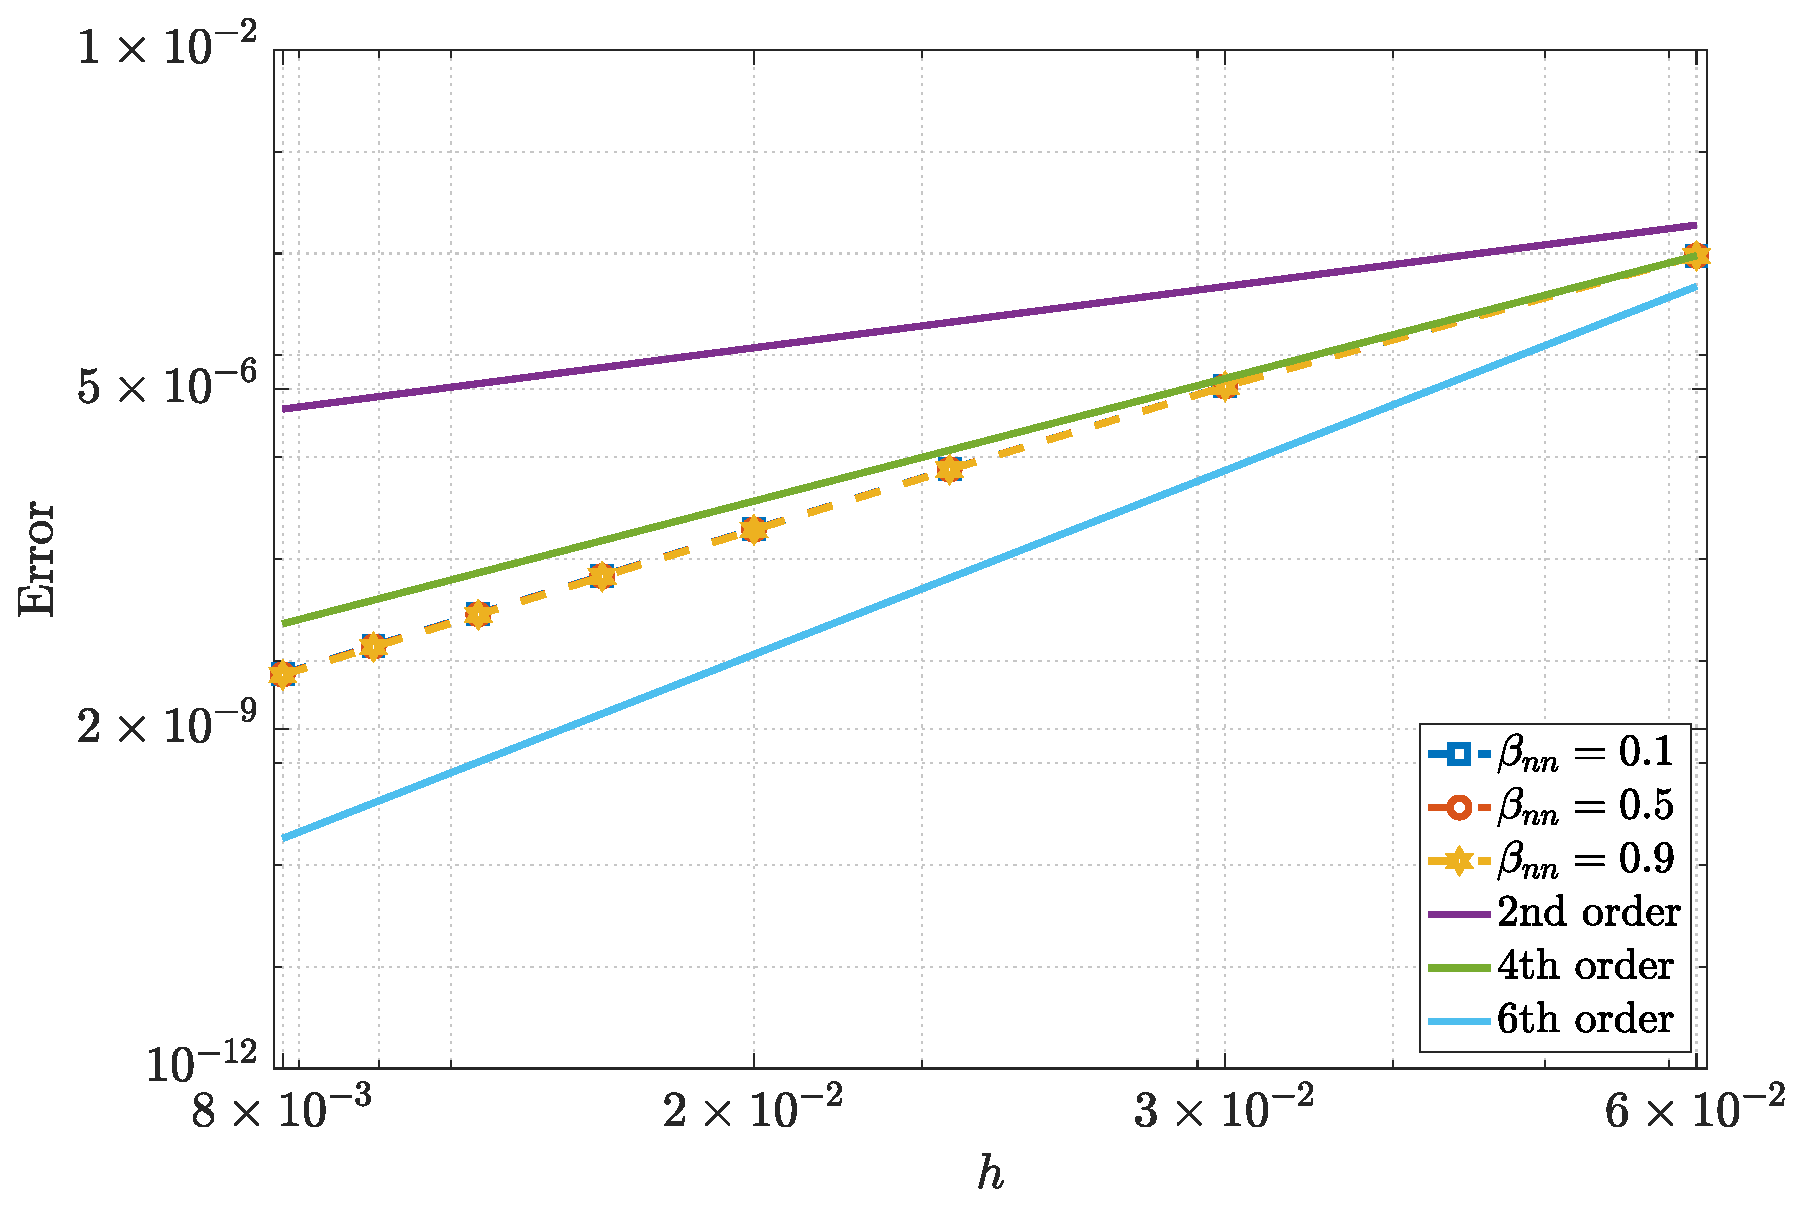
\includegraphics[width=\textwidth]{NormErr_2nd_Re_100_Wi_1_epsilon_0_xi_0_alphaG_0.1_Dt_1e-06_at_0.05_tipsim_1_MMS_12_V.eps}
        \caption{$||v - \widetilde{v}||_{2}$}
        \label{error_v_2nd_Case1_giesekus_alphaG_0.1}
    \end{subfigure}
    \qquad
    \begin{subfigure}[b]{.46\textwidth}
        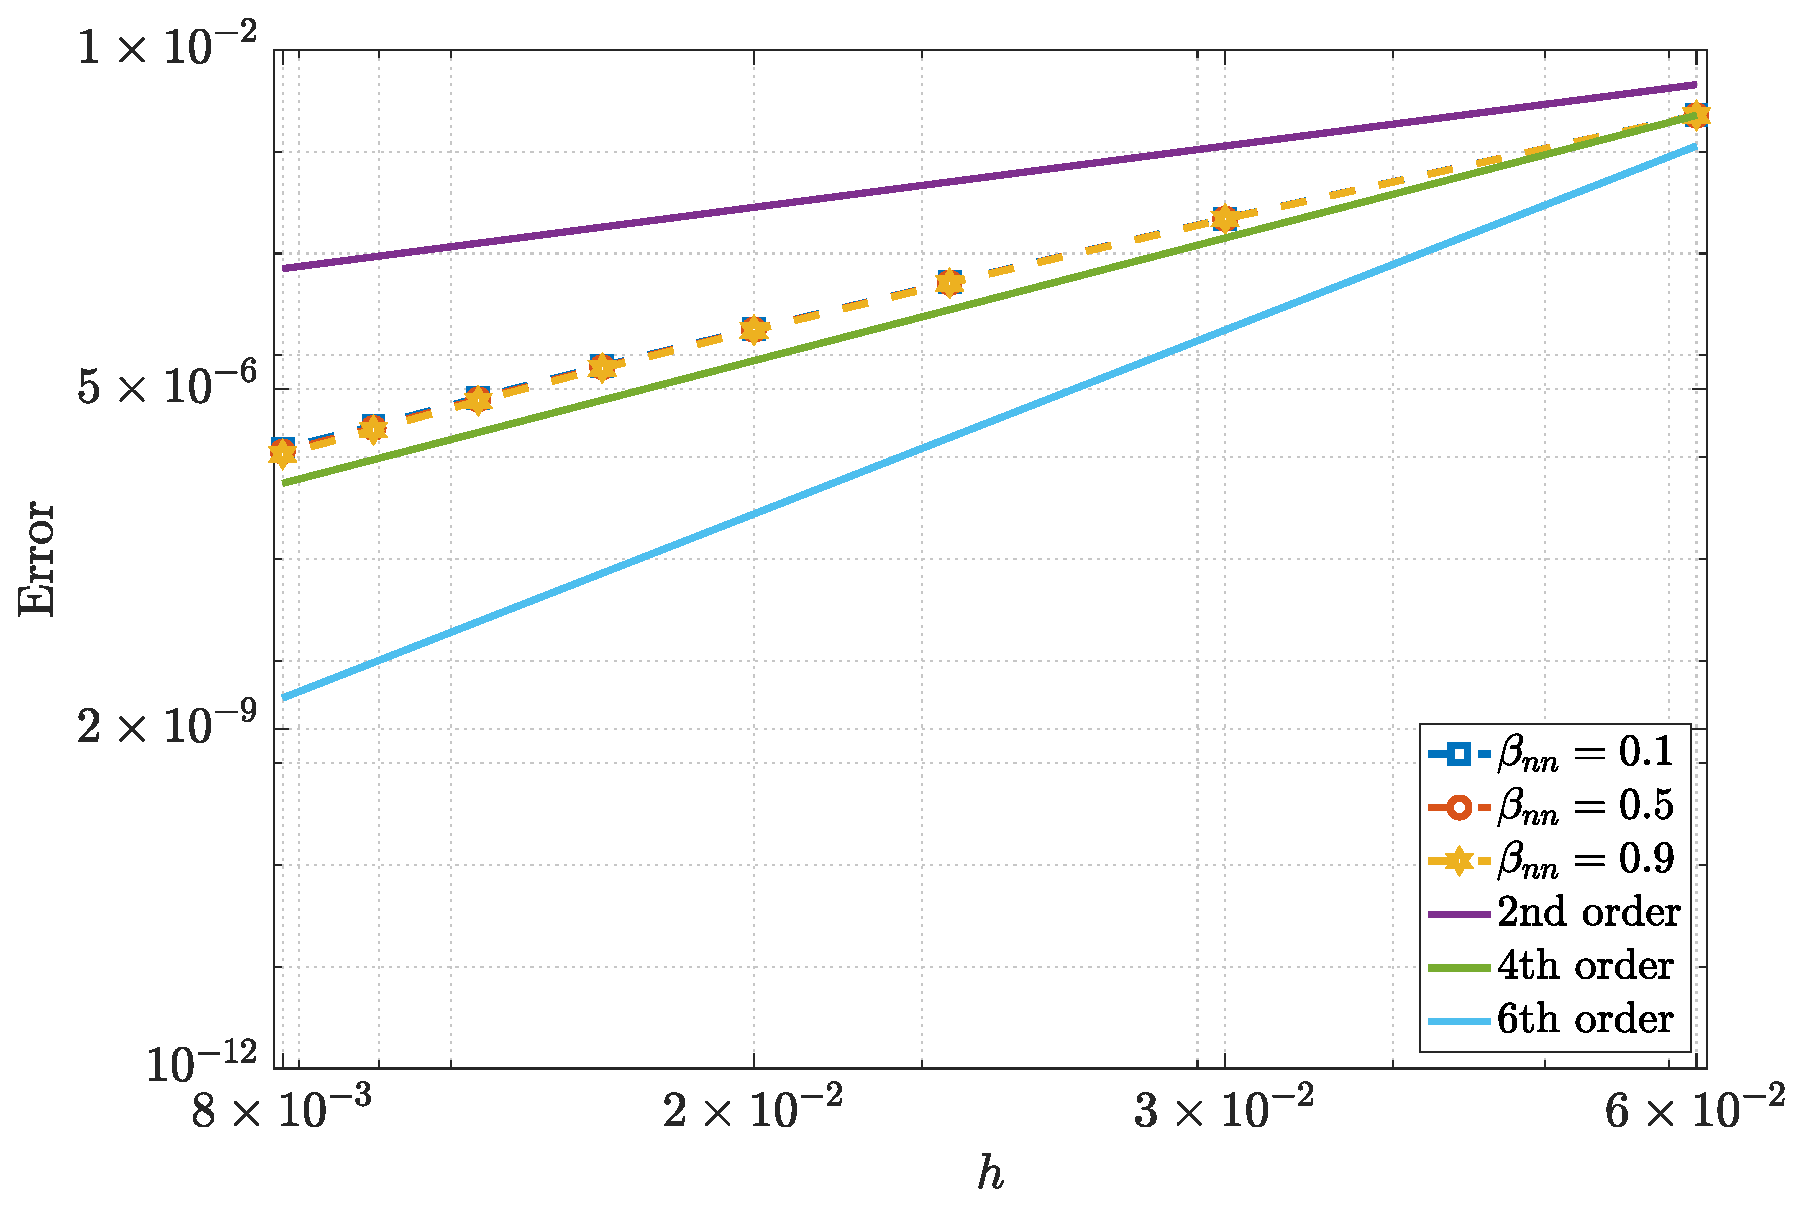
\includegraphics[width=\textwidth]{NormErr_2nd_Re_100_Wi_1_epsilon_0_xi_0_alphaG_0.1_Dt_1e-06_at_0.05_tipsim_1_MMS_12_Wz.eps}
        \caption{$||\omega_{z} - \widetilde{\omega_{z}}||_{2}$}
        \label{error_wz_2nd_Case1_giesekus_alphaG_0.1}
    \end{subfigure}
    \qquad
    \begin{subfigure}[b]{.46\textwidth}
        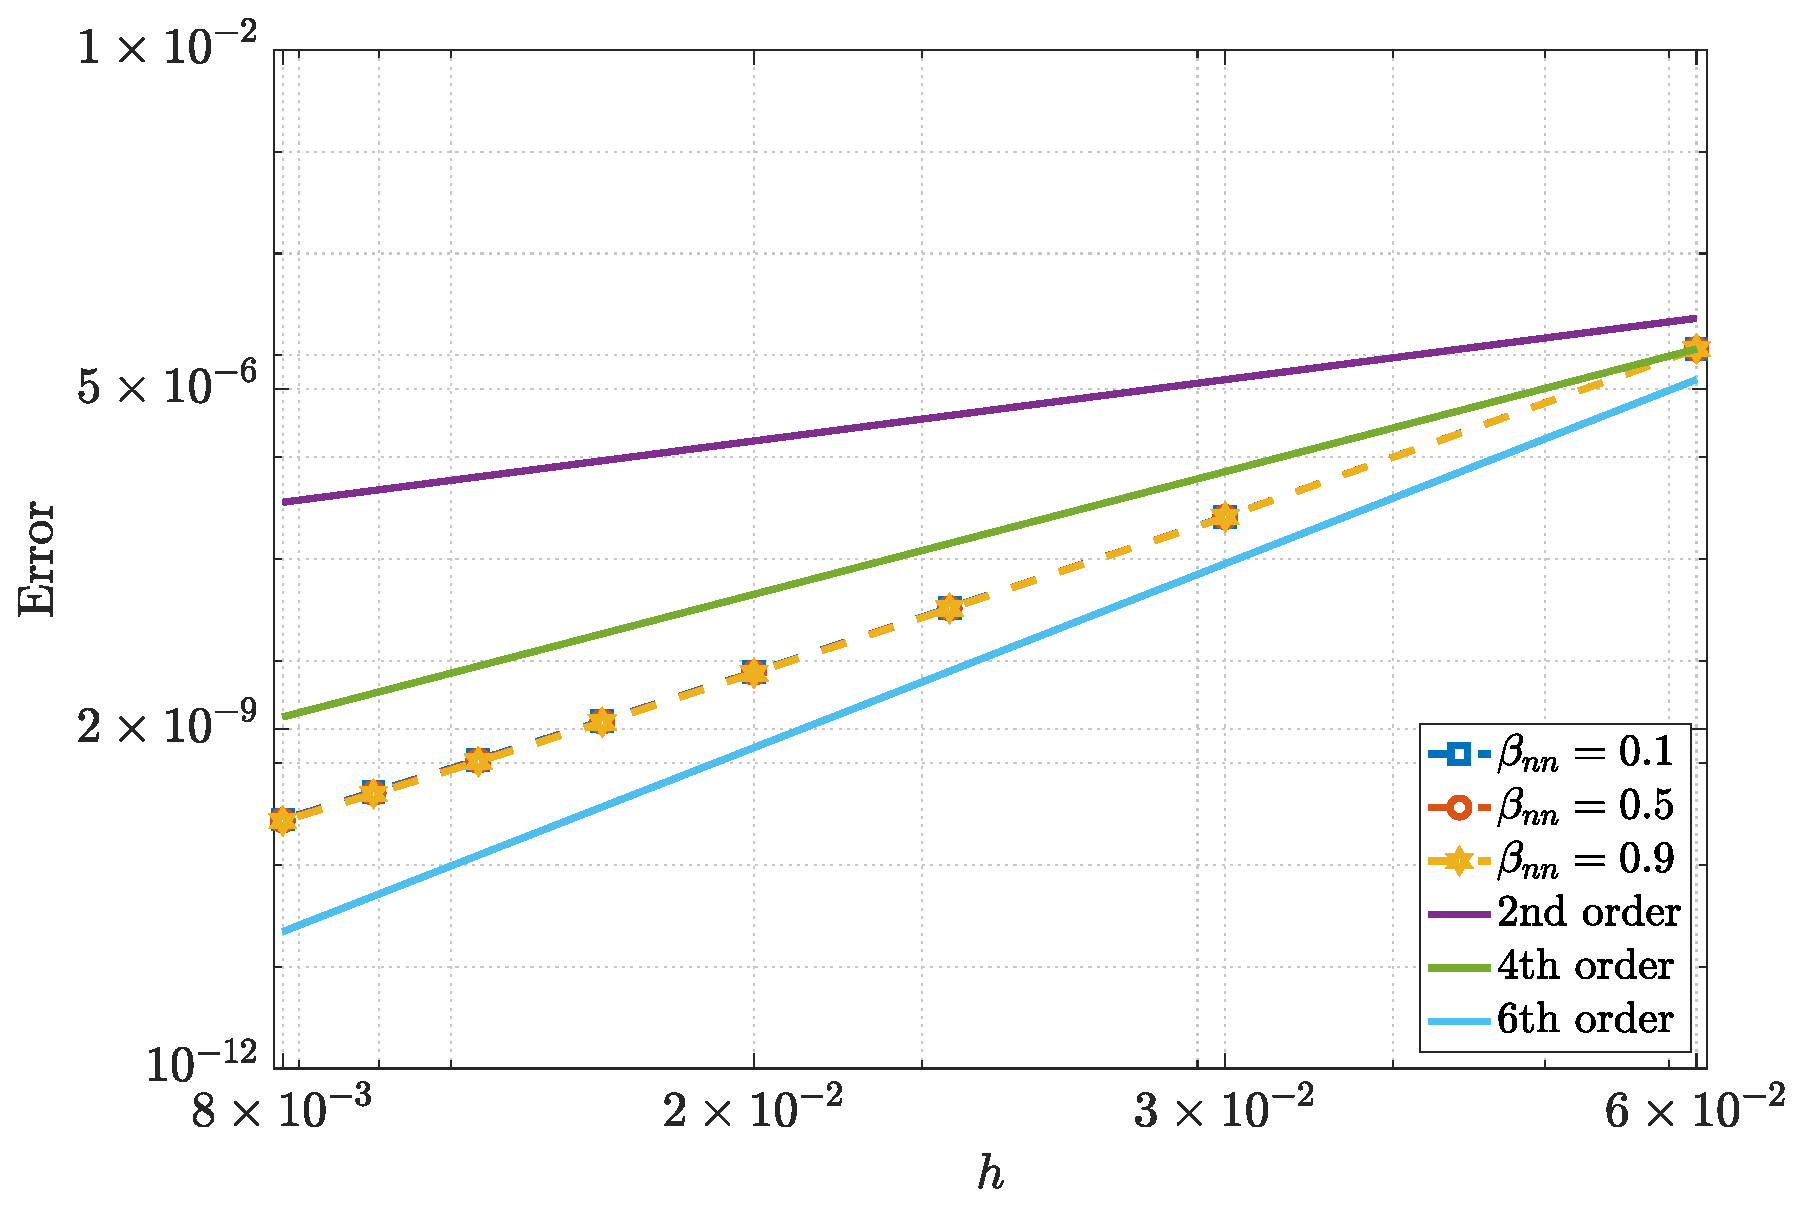
\includegraphics[width=\textwidth]{NormErr_2nd_Re_100_Wi_1_epsilon_0_xi_0_alphaG_0.1_Dt_1e-06_at_0.05_tipsim_1_MMS_12_Psi.eps}
        \caption{$||\Psi - \widetilde{\Psi}||_{2}$}
        \label{error_psi_2nd_Case1_oldorydbgiesekus_alphaG_0.1}
    \end{subfigure}
    \vspace{0.02cm}
    \caption{Error for the velocity field $({u},{v})$, vorticity $({\omega_{z}})$, and stream function $({\Psi})$, with $\operatorname{Re}=100$, $Wi=1$ and $\alpha_G=0.1$ for the Giesekus viscoelastic fluid flow, using different solvent viscosity ratios ($\beta_{nn}$) and grid sizes ($\Delta x, \Delta y$).\label{fig_Giesekus_error011}}
\end{figure}

Figure \ref{fig_Giesekus_error012} expands the analysis by presenting the
errors related to the polymeric tensor components $T_{xx}$, $T_{xy}$, and
$T_{yy}$ using different grid sizes ($\Delta x, \Delta y$), for the same set of
parameters $\operatorname{Re} = 100$, $Wi = 1$ and $\alpha_G = 0.1$. The
results show a significant reduction in errors as the mesh is refined,
maintaining a high convergence order, typically close to 4. This suggests that
the numerical method is robust in capturing the complexity of the polymeric
tensor in viscoelastic fluids, minimizing deviations between different values
of $\beta_{nn}$.

\begin{figure}[H]
    \centering  
    \begin{subfigure}[b]{.46\textwidth}
        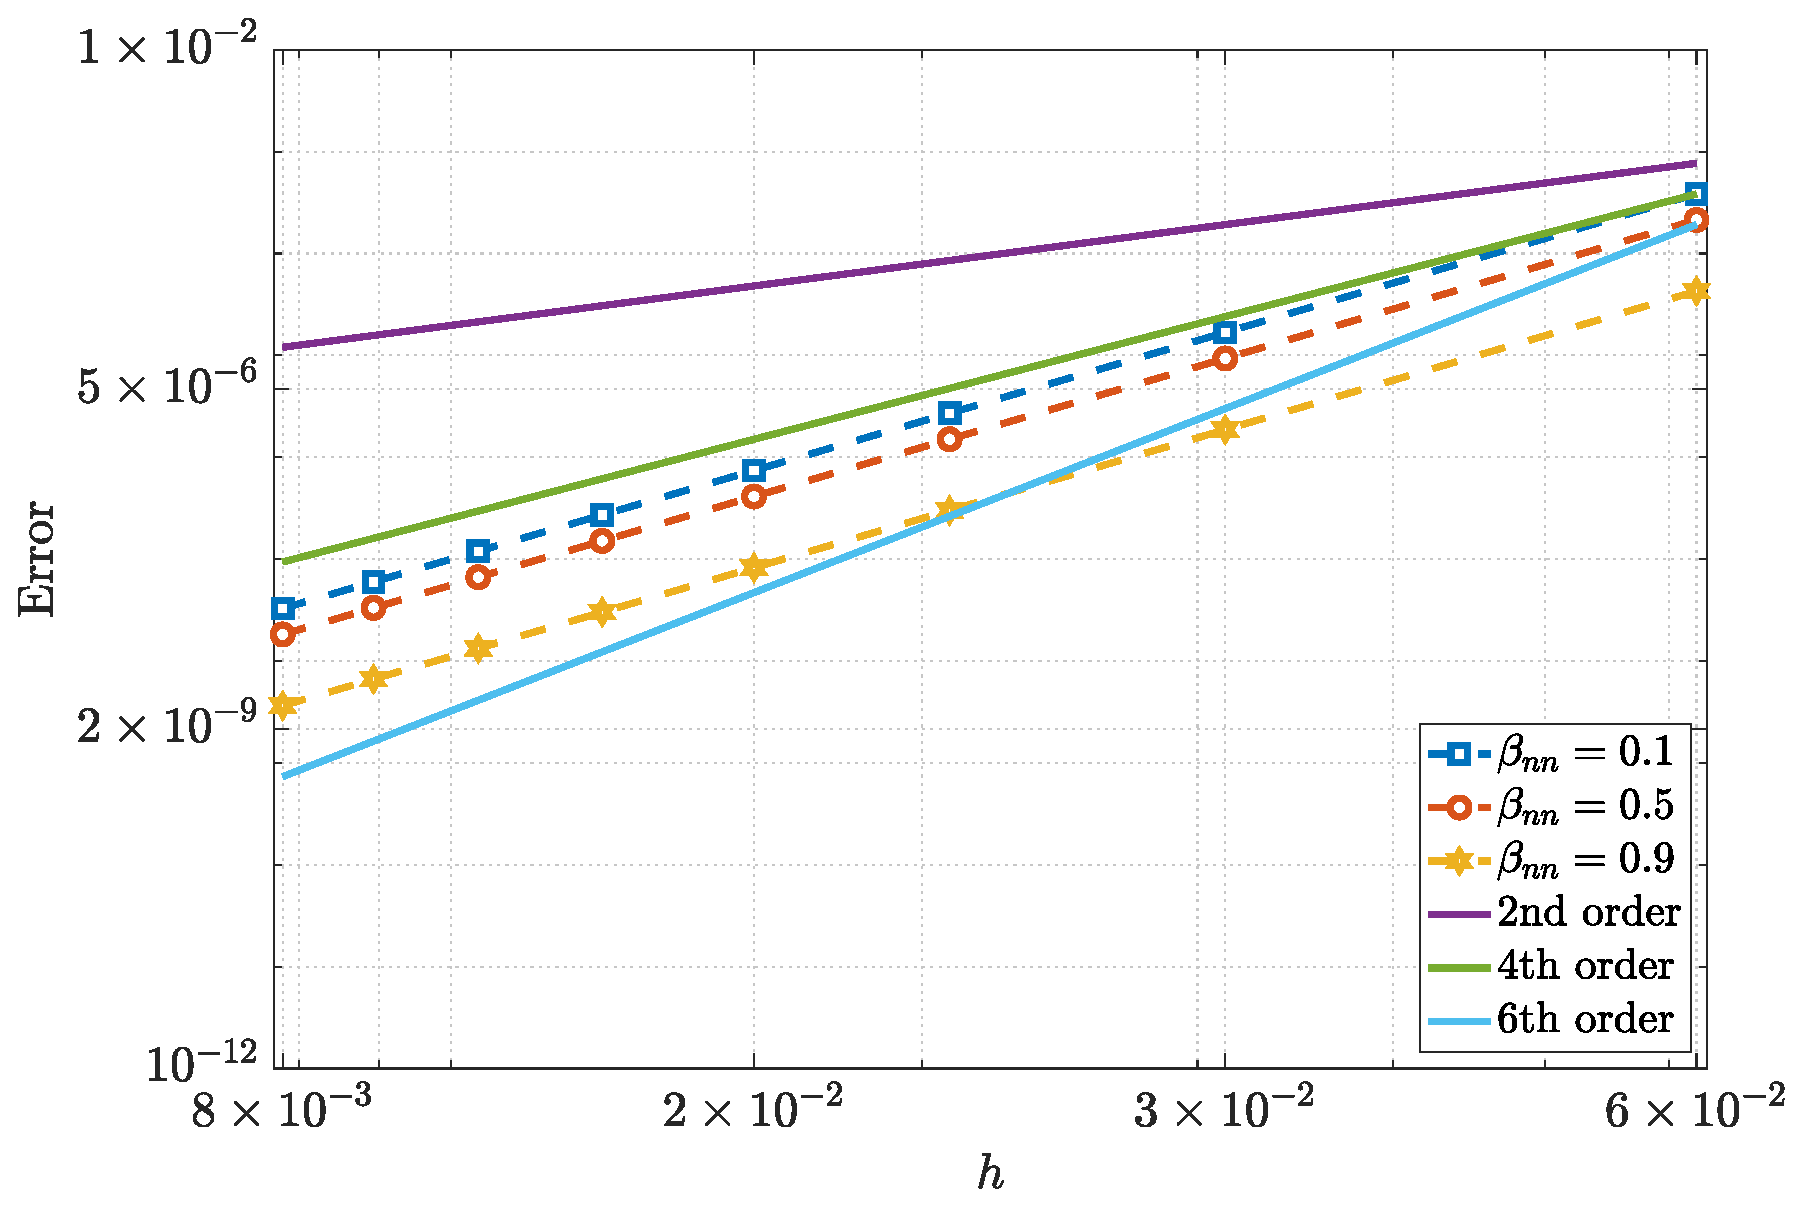
\includegraphics[width=\textwidth]{NormErr_2nd_Re_100_Wi_1_epsilon_0_xi_0_alphaG_0.1_Dt_1e-06_at_0.05_tipsim_1_MMS_12_Txx.eps}
        \caption{$||T_{xx} - \overline{T}_{xx}||_{2}$}
        \label{error_txx_2nd_Case1_giesekus_alphaG_0.1}
    \end{subfigure}
    \vspace{0.2cm}
    \qquad
    \begin{subfigure}[b]{.46\textwidth}
        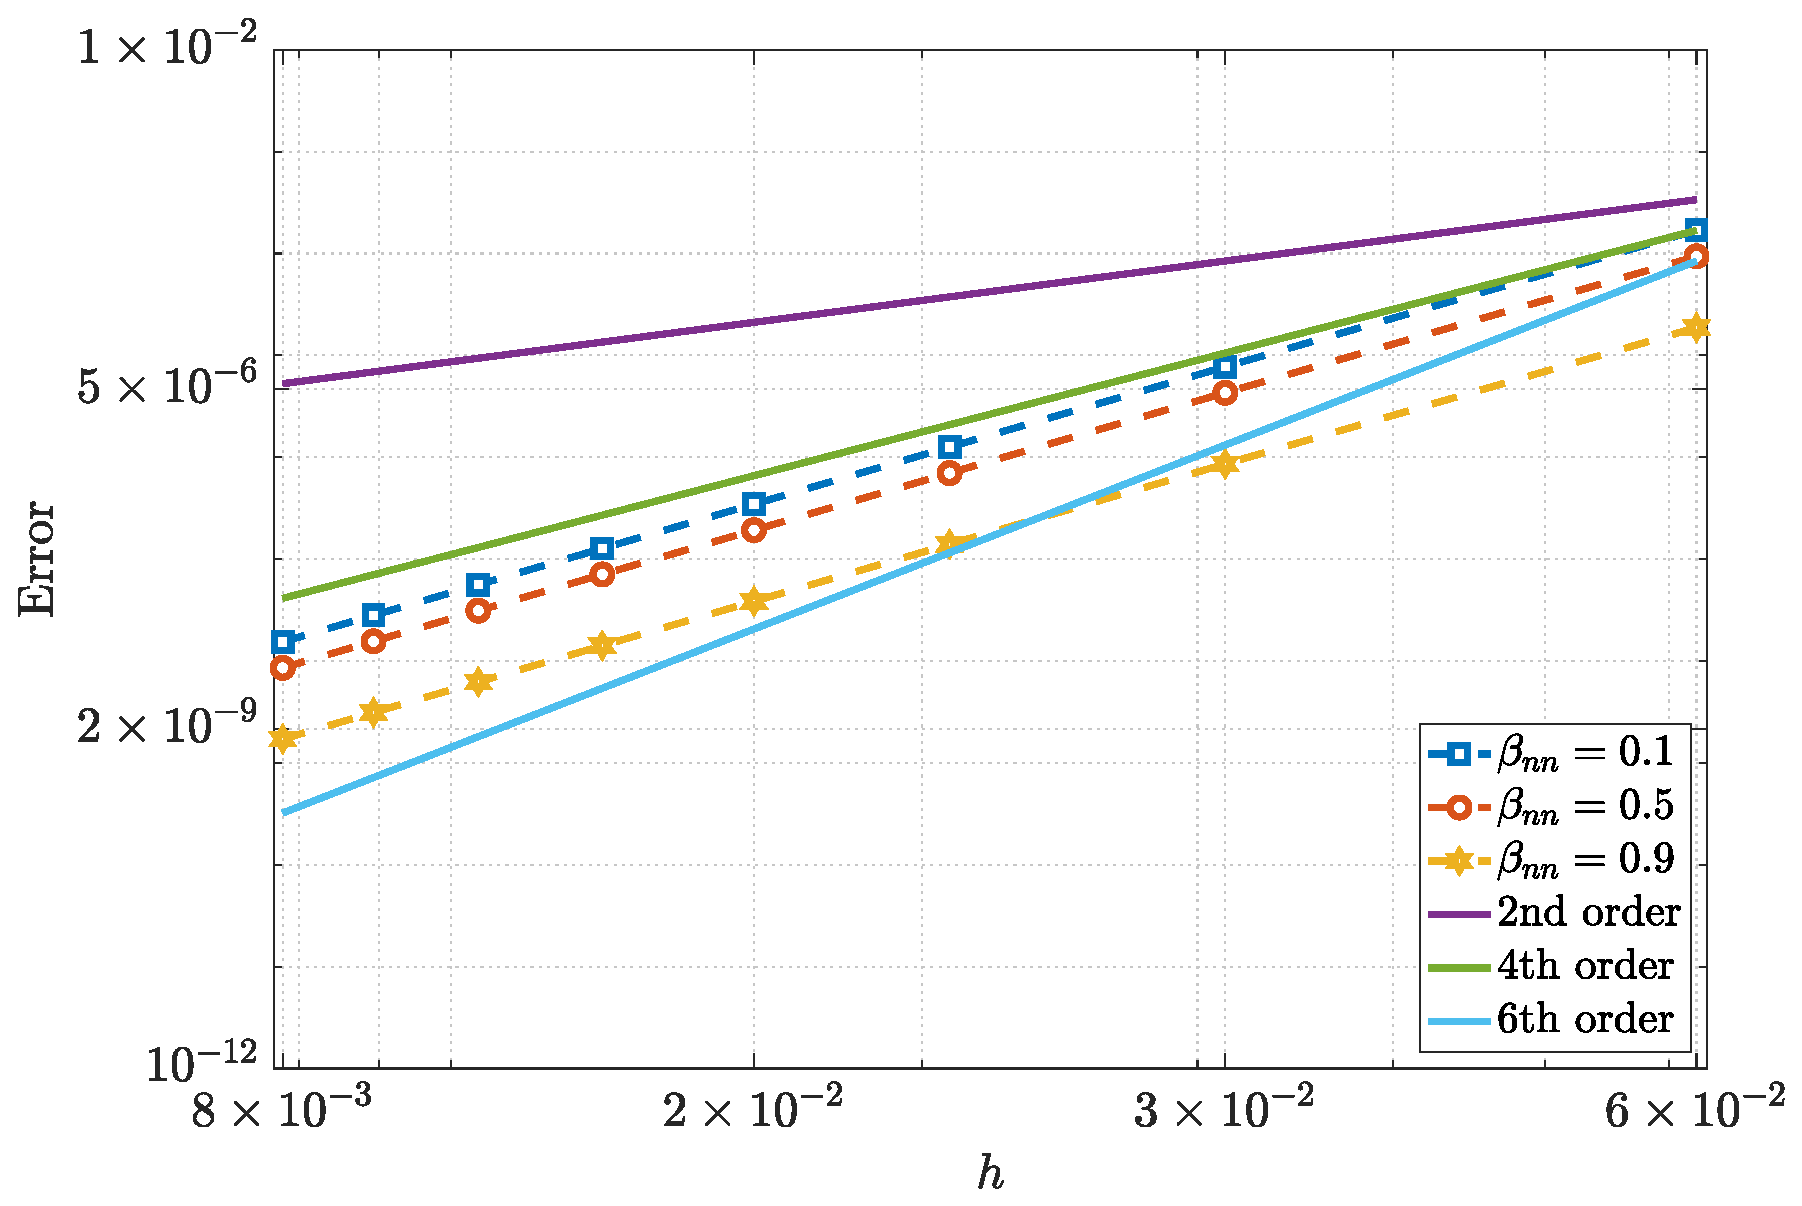
\includegraphics[width=\textwidth]{NormErr_2nd_Re_100_Wi_1_epsilon_0_xi_0_alphaG_0.1_Dt_1e-06_at_0.05_tipsim_1_MMS_12_Txy.eps}
        \caption{$||T_{xy} - \overline{T}_{xy}||_{2}$}
        \label{error_txy_2nd_Case1_giesekus_alphaG_0.1}
    \end{subfigure}
    \qquad
    \begin{subfigure}[b]{.46\textwidth}
        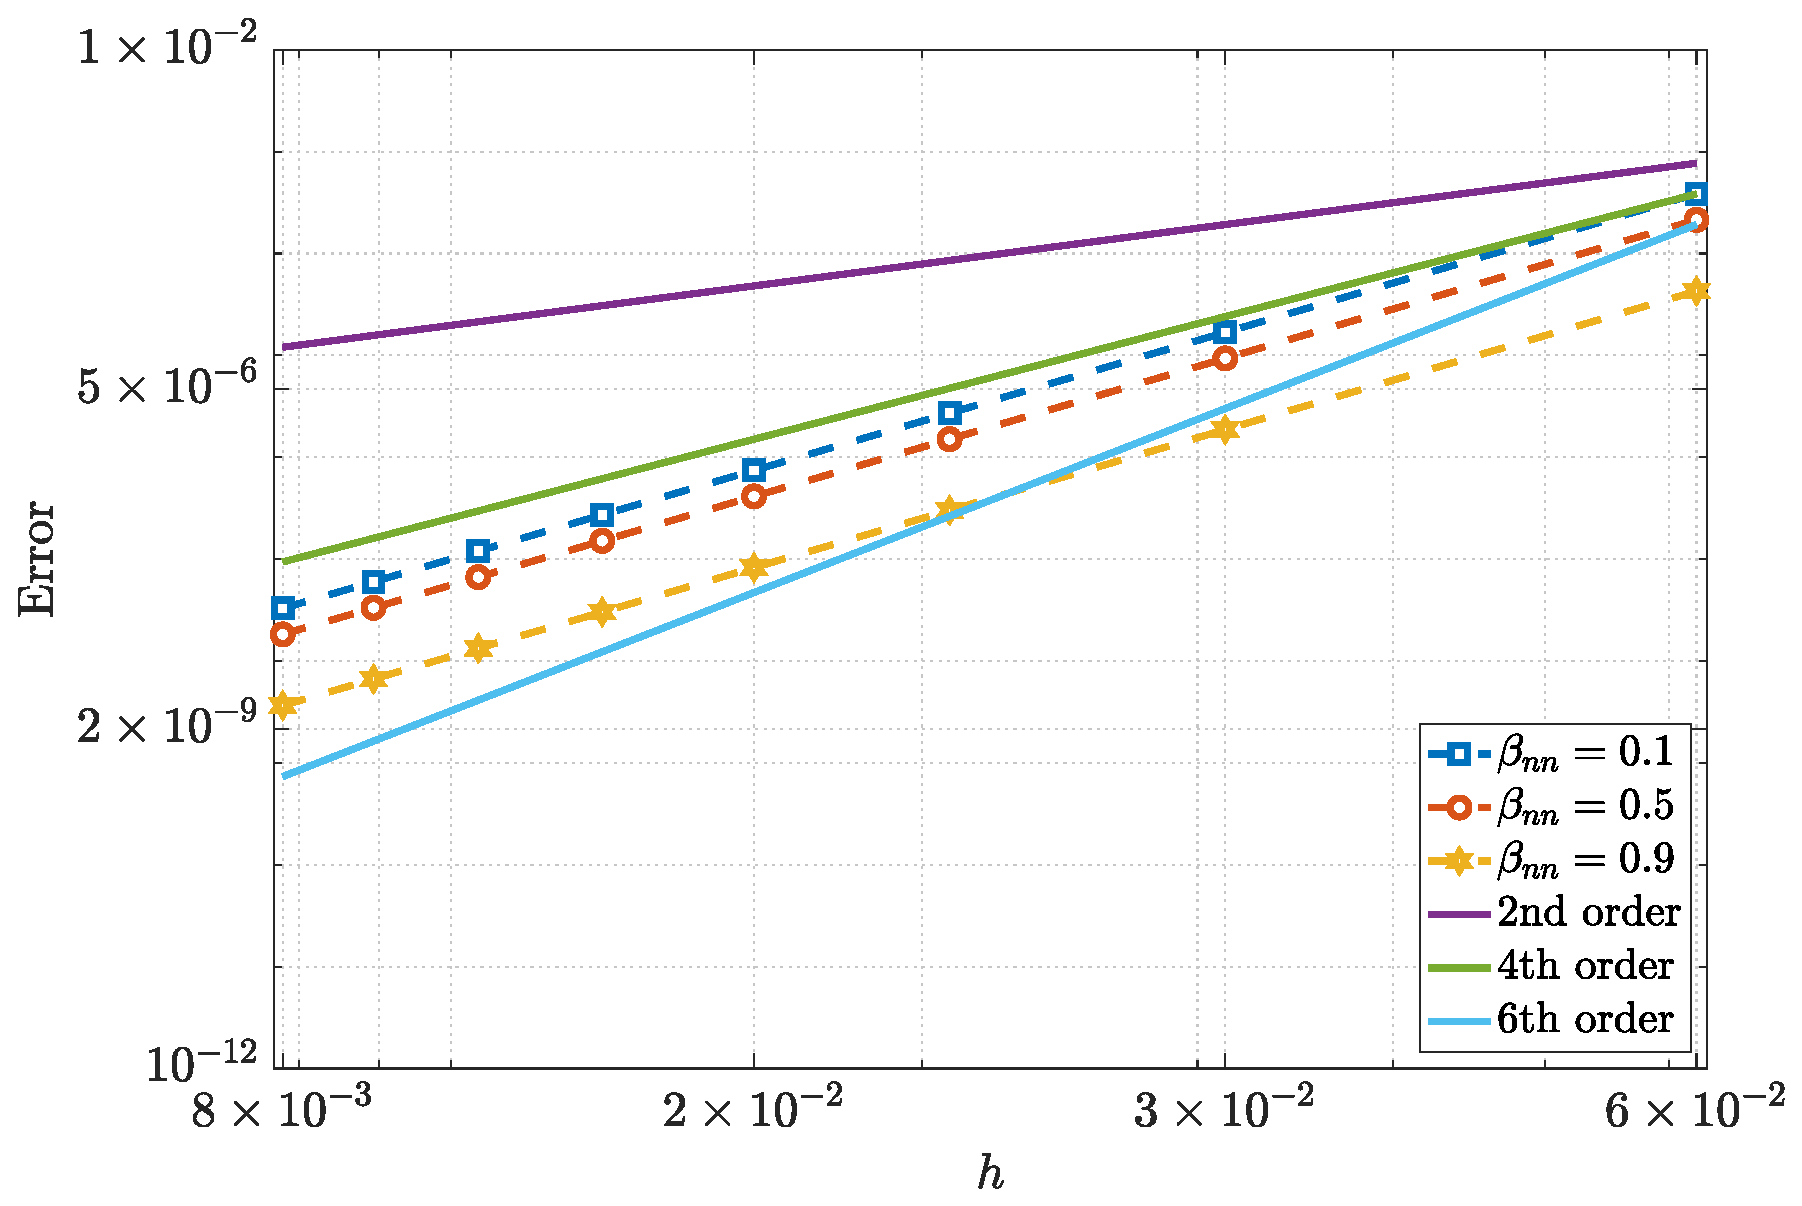
\includegraphics[width=\textwidth]{NormErr_2nd_Re_100_Wi_1_epsilon_0_xi_0_alphaG_0.1_Dt_1e-06_at_0.05_tipsim_1_MMS_12_Tyy.eps}
        \caption{$||T_{yy} - \overline{T}_{yy}||_{2}$}
        \label{error_tyy_2nd_Case1_giesekus_alphaG_0.1}
    \end{subfigure}
    \vspace{0.02cm}
    \caption{Error for the polymeric tensor components ($T_{xx}, T_{xy}, T_{yy}$), with $\operatorname{Re}=100,$ $Wi=1$ and $\alpha_{G} = 0.1$ for the Giesekus viscoelastic fluid flow, using different solvent viscosity ratios ($\beta_{nn}$) and grid sizes ($\Delta x, \Delta y$).\label{fig_Giesekus_error012}}
\end{figure}

\begin{center}
\begin{table}[H]
\caption{Numerical errors and convergence order calculation for vorticity ($\omega_{z}$), using \mbox{$Wi=1$}, $Re=\{1,100,400,1000\}$, $\beta_{nn}=\{0.1,0.5,0.9,1.0\}$ and $\alpha_G = 0.1$, for the Giesekus viscoelastic fluid flow.\label{tab_GiesekusWzalphaG01Resumida}}
\scriptsize{
    \begin{tabular*}{\textwidth}{@{\extracolsep\fill}cccccccccc@{}}
    \hline
    \multirow{2}{*}{$\operatorname{Re}$} & \multirow{2}{*}{Mesh} & \multicolumn{2}{c}{$\beta_{nn}=0.1$}  & \multicolumn{2}{c}{$\beta_{nn}=0.5$}  & \multicolumn{2}{c}{$\beta_{nn}=0.9$}  & \multicolumn{2}{c}{$\beta_{nn}=1.0$}\\ %\cline{3-10}
     & & Error & Order & Error & Order & Error & Order & Error & Order \\
    \hline
    \multirow{7}{*}{1.00} & $17\times 17$ & 2.23e-03 & --- & 2.08e-03 & --- & 1.96e-03 & --- & 1.93e-03 & --- \\
    & $33\times 33$ & 2.02e-04 & 3.47 & 1.51e-04 & 3.79 & 1.23e-04 & 4.00 & 1.18e-04 & 4.03 \\
    & $49\times 49$ & 4.26e-05 & 3.84 & 2.50e-05 & 4.44 & 1.92e-05 & 4.57 & 1.84e-05 & 4.58 \\
    & $65\times 65$ & 1.28e-05 & 4.17 & 6.43e-06 & 4.71 & 5.05e-06 & 4.65 & 4.85e-06 & 4.63 \\
    & $81\times 81$ & 4.68e-06 & 4.52 & 2.23e-06 & 4.74 & 1.79e-06 & 4.63 & 1.73e-06 & 4.61 \\
    & $97\times 97$ & 1.92e-06 & 4.90 & 9.34e-07 & 4.78 & 7.68e-07 & 4.65 & 7.45e-07 & 4.63 \\
    & $113\times 113$ & 8.58e-07 & 5.21 & 4.47e-07 & 4.77 & 3.80e-07 & 4.57 & 3.71e-07 & 4.52 \\
    & $129\times 129$ & 4.34e-07 & 5.10 & 2.59e-07 & 4.11 & 2.30e-07 & 3.76 & 2.26e-07 & 3.71 \\
    \hline\hline
    \multirow{7}{*}{100.00} & $17\times 17$ & 2.27e-03 & --- & 2.27e-03 & --- & 2.26e-03 & --- & 2.26e-03 & --- \\
    & $33\times 33$ & 2.20e-04 & 3.37 & 2.19e-04 & 3.37 & 2.18e-04 & 3.37 & 2.18e-04 & 3.37 \\
    & $49\times 49$ & 5.20e-05 & 3.56 & 5.15e-05 & 3.57 & 5.11e-05 & 3.58 & 5.10e-05 & 3.59 \\
    & $65\times 65$ & 1.82e-05 & 3.66 & 1.79e-05 & 3.68 & 1.76e-05 & 3.70 & 1.75e-05 & 3.71 \\
    & $81\times 81$ & 7.84e-06 & 3.76 & 7.65e-06 & 3.80 & 7.47e-06 & 3.84 & 7.43e-06 & 3.85 \\
    & $97\times 97$ & 3.83e-06 & 3.93 & 3.70e-06 & 3.99 & 3.57e-06 & 4.05 & 3.54e-06 & 4.06 \\
    & $113\times 113$ & 2.04e-06 & 4.10 & 1.94e-06 & 4.19 & 1.85e-06 & 4.27 & 1.83e-06 & 4.29 \\
    & $129\times 129$ & 1.21e-06 & 3.89 & 1.13e-06 & 4.02 & 1.07e-06 & 4.13 & 1.05e-06 & 4.16 \\
    \hline\hline
    \multirow{7}{*}{400.00} & $17\times 17$ & 2.27e-03 & --- & 2.27e-03 & --- & 2.27e-03 & --- & 2.27e-03 & --- \\
    & $33\times 33$ & 2.20e-04 & 3.37 & 2.20e-04 & 3.37 & 2.20e-04 & 3.37 & 2.20e-04 & 3.37 \\
    & $49\times 49$ & 5.21e-05 & 3.56 & 5.19e-05 & 3.56 & 5.18e-05 & 3.56 & 5.18e-05 & 3.56 \\
    & $65\times 65$ & 1.82e-05 & 3.65 & 1.81e-05 & 3.66 & 1.81e-05 & 3.66 & 1.81e-05 & 3.66 \\
    & $81\times 81$ & 7.88e-06 & 3.75 & 7.83e-06 & 3.76 & 7.79e-06 & 3.77 & 7.78e-06 & 3.77 \\
    & $97\times 97$ & 3.86e-06 & 3.92 & 3.83e-06 & 3.93 & 3.80e-06 & 3.94 & 3.79e-06 & 3.95 \\
    & $113\times 113$ & 2.05e-06 & 4.09 & 2.03e-06 & 4.11 & 2.01e-06 & 4.12 & 2.01e-06 & 4.13 \\
    & $129\times 129$ & 1.23e-06 & 3.86 & 1.21e-06 & 3.89 & 1.19e-06 & 3.92 & 1.19e-06 & 3.93 \\
    \hline\hline
    \multirow{7}{*}{1000.00} & $17\times 17$ & 2.27e-03 & --- & 2.27e-03 & --- & 2.27e-03 & --- & 2.27e-03 & --- \\
    & $33\times 33$ & 2.20e-04 & 3.37 & 2.20e-04 & 3.37 & 2.20e-04 & 3.37 & 2.20e-04 & 3.37 \\
    & $49\times 49$ & 5.21e-05 & 3.56 & 5.20e-05 & 3.56 & 5.20e-05 & 3.56 & 5.20e-05 & 3.56 \\
    & $65\times 65$ & 1.82e-05 & 3.65 & 1.82e-05 & 3.65 & 1.82e-05 & 3.65 & 1.82e-05 & 3.65 \\
    & $81\times 81$ & 7.89e-06 & 3.75 & 7.87e-06 & 3.76 & 7.86e-06 & 3.76 & 7.85e-06 & 3.76 \\
    & $97\times 97$ & 3.86e-06 & 3.92 & 3.85e-06 & 3.92 & 3.84e-06 & 3.92 & 3.84e-06 & 3.92 \\
    & $113\times 113$ & 2.06e-06 & 4.08 & 2.05e-06 & 4.09 & 2.04e-06 & 4.09 & 2.04e-06 & 4.09 \\
    & $129\times 129$ & 1.23e-06 & 3.86 & 1.22e-06 & 3.87 & 1.22e-06 & 3.87 & 1.22e-06 & 3.88 \\
    \hline
    \end{tabular*}
}
\end{table}
\end{center}

\begin{center}
\begin{table}[H]
\caption{Numerical errors and convergence order calculation for the polymeric tensor component $T_{xy}$, using \mbox{$Wi=1$}, $Re=\{1,100,400,1000\}$, $\beta_{nn}=\{0.1,0.5,0.9,1.0\}$ and \mbox{$\alpha_G = 0.1$}, for the Giesekus viscoelastic fluid flow.\label{tab_GiesekusTxyalphaG01Resumida}}
\scriptsize{
    \begin{tabular*}{\textwidth}{@{\extracolsep\fill}cccccccccc@{}}
    \hline
    \multirow{2}{*}{$\operatorname{Re}$} & \multirow{2}{*}{Mesh} & \multicolumn{2}{c}{$\beta_{nn}=0.1$}  & \multicolumn{2}{c}{$\beta_{nn}=0.5$}  & \multicolumn{2}{c}{$\beta_{nn}=0.9$}  & \multicolumn{2}{c}{$\beta_{nn}=1.0$}\\ %\cline{3-10}
     & & Error & Order & Error & Order & Error & Order & Error & Order \\
    \hline
    \multirow{7}{*}{1.00} & $17\times 17$ & 1.70e-04 & --- & 9.43e-05 & --- & 1.89e-05 & --- & 1.89e-18 & --- \\
    & $33\times 33$ & 7.77e-06 & 4.45 & 4.32e-06 & 4.45 & 8.64e-07 & 4.45 & 8.63e-20 & 4.45 \\
    & $49\times 49$ & 1.27e-06 & 4.48 & 7.04e-07 & 4.48 & 1.41e-07 & 4.48 & 1.41e-20 & 4.48 \\
    & $65\times 65$ & 3.49e-07 & 4.48 & 1.94e-07 & 4.48 & 3.87e-08 & 4.48 & 3.87e-21 & 4.48 \\
    & $81\times 81$ & 1.28e-07 & 4.49 & 7.11e-08 & 4.49 & 1.42e-08 & 4.49 & 1.42e-21 & 4.49 \\
    & $97\times 97$ & 5.65e-08 & 4.49 & 3.14e-08 & 4.49 & 6.28e-09 & 4.49 & 6.27e-22 & 4.49 \\
    & $113\times 113$ & 2.83e-08 & 4.49 & 1.57e-08 & 4.49 & 3.14e-09 & 4.49 & 3.14e-22 & 4.49 \\
    & $129\times 129$ & 1.55e-08 & 4.49 & 8.62e-09 & 4.49 & 1.72e-09 & 4.49 & 1.72e-22 & 4.49 \\
    \hline\hline
    \multirow{7}{*}{100.00} & $17\times 17$ & 1.69e-04 & --- & 9.37e-05 & --- & 1.87e-05 & --- & 1.87e-18 & --- \\
    & $33\times 33$ & 7.73e-06 & 4.45 & 4.29e-06 & 4.45 & 8.59e-07 & 4.45 & 8.58e-20 & 4.45 \\
    & $49\times 49$ & 1.26e-06 & 4.48 & 6.99e-07 & 4.48 & 1.40e-07 & 4.48 & 1.40e-20 & 4.48 \\
    & $65\times 65$ & 3.46e-07 & 4.48 & 1.92e-07 & 4.48 & 3.85e-08 & 4.48 & 3.85e-21 & 4.48 \\
    & $81\times 81$ & 1.27e-07 & 4.49 & 7.07e-08 & 4.49 & 1.41e-08 & 4.49 & 1.41e-21 & 4.49 \\
    & $97\times 97$ & 5.61e-08 & 4.49 & 3.12e-08 & 4.49 & 6.24e-09 & 4.49 & 6.23e-22 & 4.49 \\
    & $113\times 113$ & 2.81e-08 & 4.49 & 1.56e-08 & 4.49 & 3.12e-09 & 4.49 & 3.12e-22 & 4.49 \\
    & $129\times 129$ & 1.54e-08 & 4.49 & 8.56e-09 & 4.49 & 1.71e-09 & 4.49 & 1.71e-22 & 4.49 \\
    \hline\hline
    \multirow{7}{*}{400.00} & $17\times 17$ & 1.66e-04 & --- & 9.20e-05 & --- & 1.84e-05 & --- & 1.84e-18 & --- \\
    & $33\times 33$ & 7.59e-06 & 4.45 & 4.22e-06 & 4.45 & 8.44e-07 & 4.45 & 8.43e-20 & 4.45 \\
    & $49\times 49$ & 1.24e-06 & 4.48 & 6.87e-07 & 4.48 & 1.37e-07 & 4.48 & 1.37e-20 & 4.48 \\
    & $65\times 65$ & 3.40e-07 & 4.48 & 1.89e-07 & 4.48 & 3.78e-08 & 4.48 & 3.78e-21 & 4.48 \\
    & $81\times 81$ & 1.25e-07 & 4.49 & 6.95e-08 & 4.49 & 1.39e-08 & 4.49 & 1.39e-21 & 4.49 \\
    & $97\times 97$ & 5.52e-08 & 4.49 & 3.06e-08 & 4.49 & 6.13e-09 & 4.49 & 6.13e-22 & 4.49 \\
    & $113\times 113$ & 2.76e-08 & 4.49 & 1.53e-08 & 4.49 & 3.07e-09 & 4.49 & 3.07e-22 & 4.49 \\
    & $129\times 129$ & 1.52e-08 & 4.49 & 8.42e-09 & 4.49 & 1.68e-09 & 4.49 & 1.68e-22 & 4.49 \\
    \hline\hline
    \multirow{7}{*}{1000.00} & $17\times 17$ & 1.60e-04 & --- & 8.90e-05 & --- & 1.78e-05 & --- & 1.78e-18 & --- \\
    & $33\times 33$ & 7.36e-06 & 4.44 & 4.09e-06 & 4.44 & 8.18e-07 & 4.44 & 8.18e-20 & 4.44 \\
    & $49\times 49$ & 1.20e-06 & 4.47 & 6.67e-07 & 4.47 & 1.33e-07 & 4.47 & 1.33e-20 & 4.47 \\
    & $65\times 65$ & 3.31e-07 & 4.48 & 1.84e-07 & 4.48 & 3.67e-08 & 4.48 & 3.67e-21 & 4.48 \\
    & $81\times 81$ & 1.21e-07 & 4.49 & 6.75e-08 & 4.49 & 1.35e-08 & 4.49 & 1.35e-21 & 4.49 \\
    & $97\times 97$ & 5.36e-08 & 4.49 & 2.98e-08 & 4.49 & 5.95e-09 & 4.49 & 5.95e-22 & 4.49 \\
    & $113\times 113$ & 2.68e-08 & 4.49 & 1.49e-08 & 4.49 & 2.98e-09 & 4.49 & 2.98e-22 & 4.49 \\
    & $129\times 129$ & 1.47e-08 & 4.49 & 8.18e-09 & 4.49 & 1.64e-09 & 4.49 & 1.64e-22 & 4.49 \\
    \hline
    \end{tabular*}
}
\end{table}
\end{center}

Tables~\ref{tab_GiesekusWzalphaG01Resumida} and \ref{tab_GiesekusTxyalphaG01Resumida} present the errors and convergence order for vorticity ($\omega_z$) and the polymeric tensor component $T_{xy}$, respectively, using $Wi = 1$,~$Re=\{1,100,400,1000\}$,~$\beta_{nn}=\{0.1,0.5,0.9,1\}$ and $\alpha_G = 0.1$. The results obtained demonstrate that as the mesh is refined, the errors decrease significantly, while the convergence order remains close to 4.5. This confirms that the numerical scheme is efficient in capturing the flow properties even on finer meshes, ensuring an accurate representation of both vorticity and polymeric tensor components even for shear-thinning viscoelastic fluid flows.

\begin{figure}[H]
    \centering  
    \begin{subfigure}[b]{.46\textwidth}
        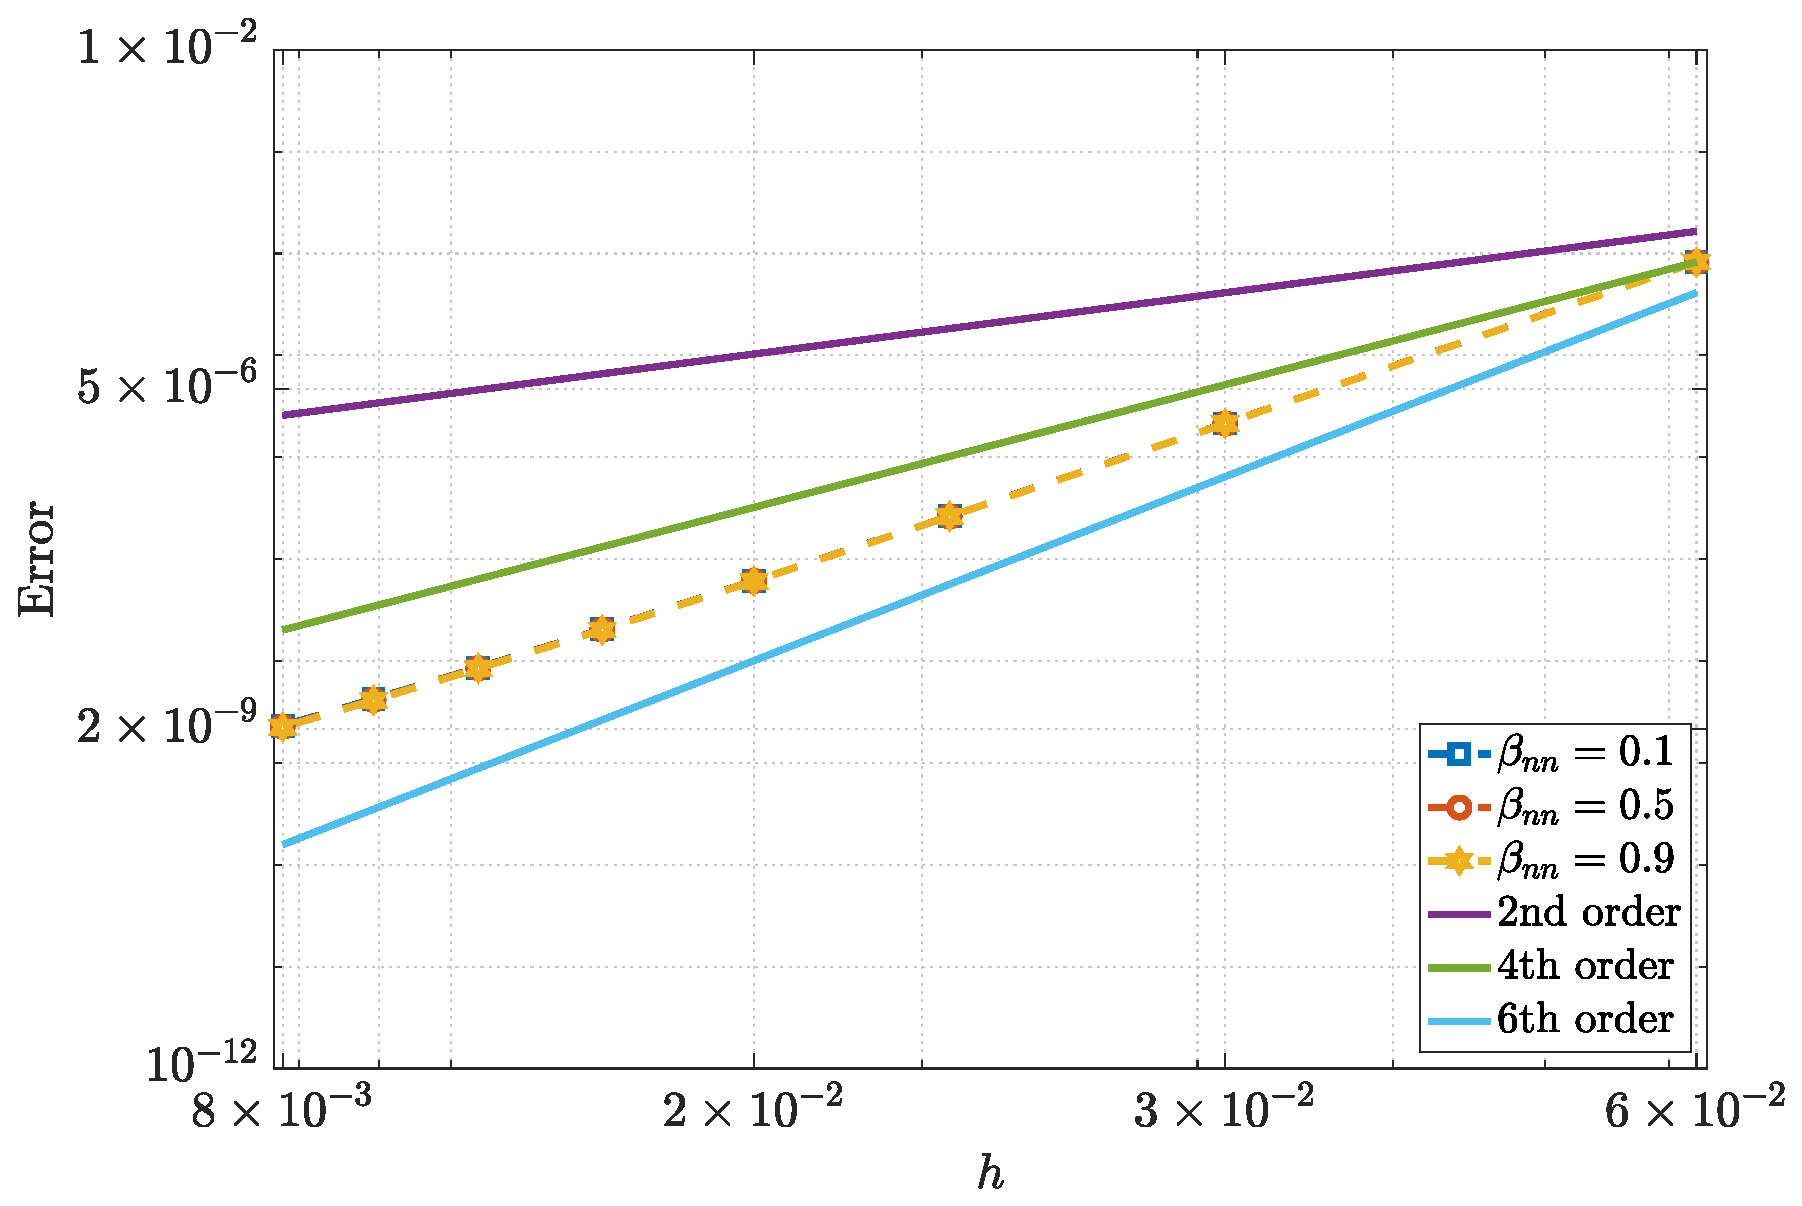
\includegraphics[width=\textwidth]{NormErr_2nd_Re_100_Wi_1_epsilon_0_xi_0_alphaG_0.5_Dt_1e-06_at_0.05_tipsim_1_MMS_12_U.eps}
        \caption{$||u - \overline{u}||_{2}$}
        \label{error_u_2nd_Case1_giesekus_alphaG_0.5}
    \end{subfigure}
    \vspace{0.2cm}
    \qquad
    \begin{subfigure}[b]{.46\textwidth}
        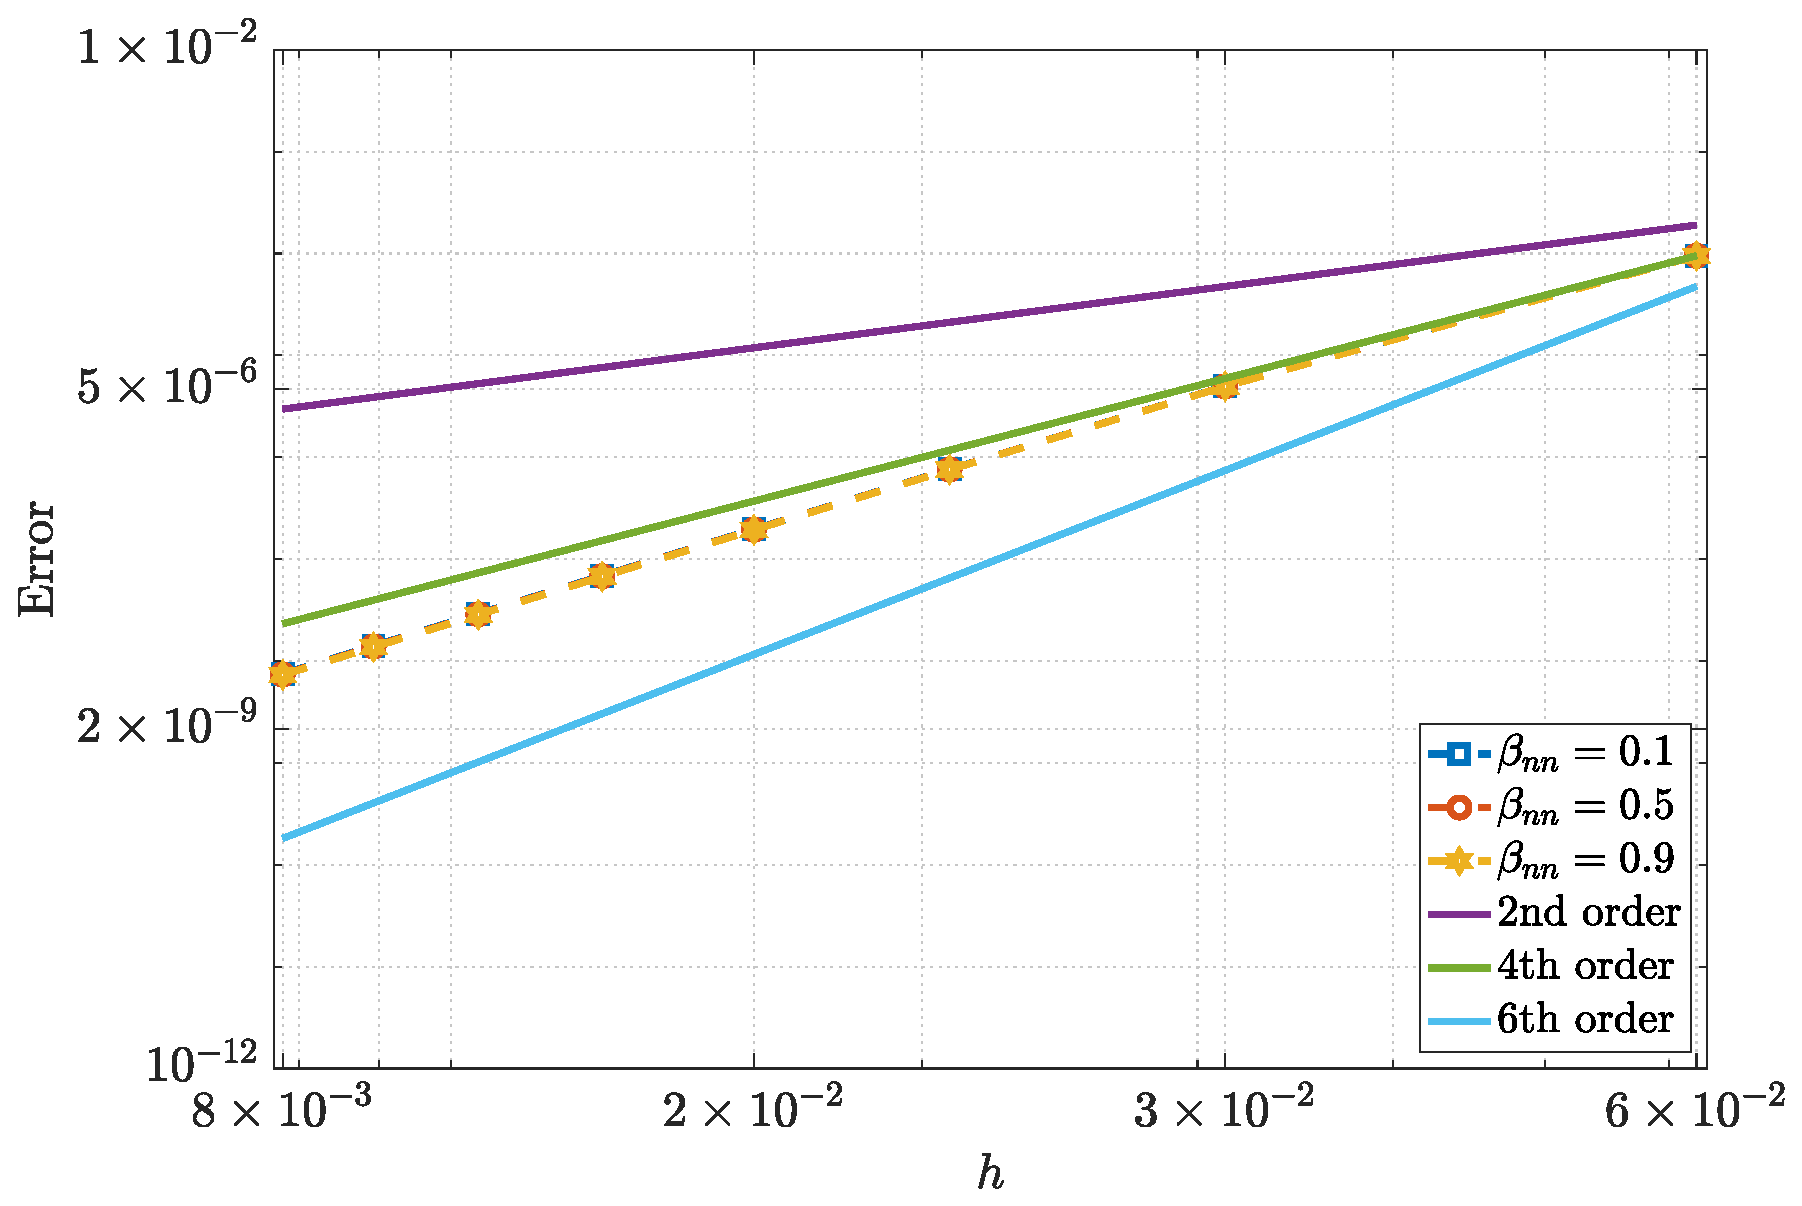
\includegraphics[width=\textwidth]{NormErr_2nd_Re_100_Wi_1_epsilon_0_xi_0_alphaG_0.5_Dt_1e-06_at_0.05_tipsim_1_MMS_12_V.eps}
        \caption{$||v - \widetilde{v}||_{2}$}
        \label{error_v_2nd_Case1_giesekus_alphaG_0.5}
    \end{subfigure}
    \qquad
    \begin{subfigure}[b]{.46\textwidth}
        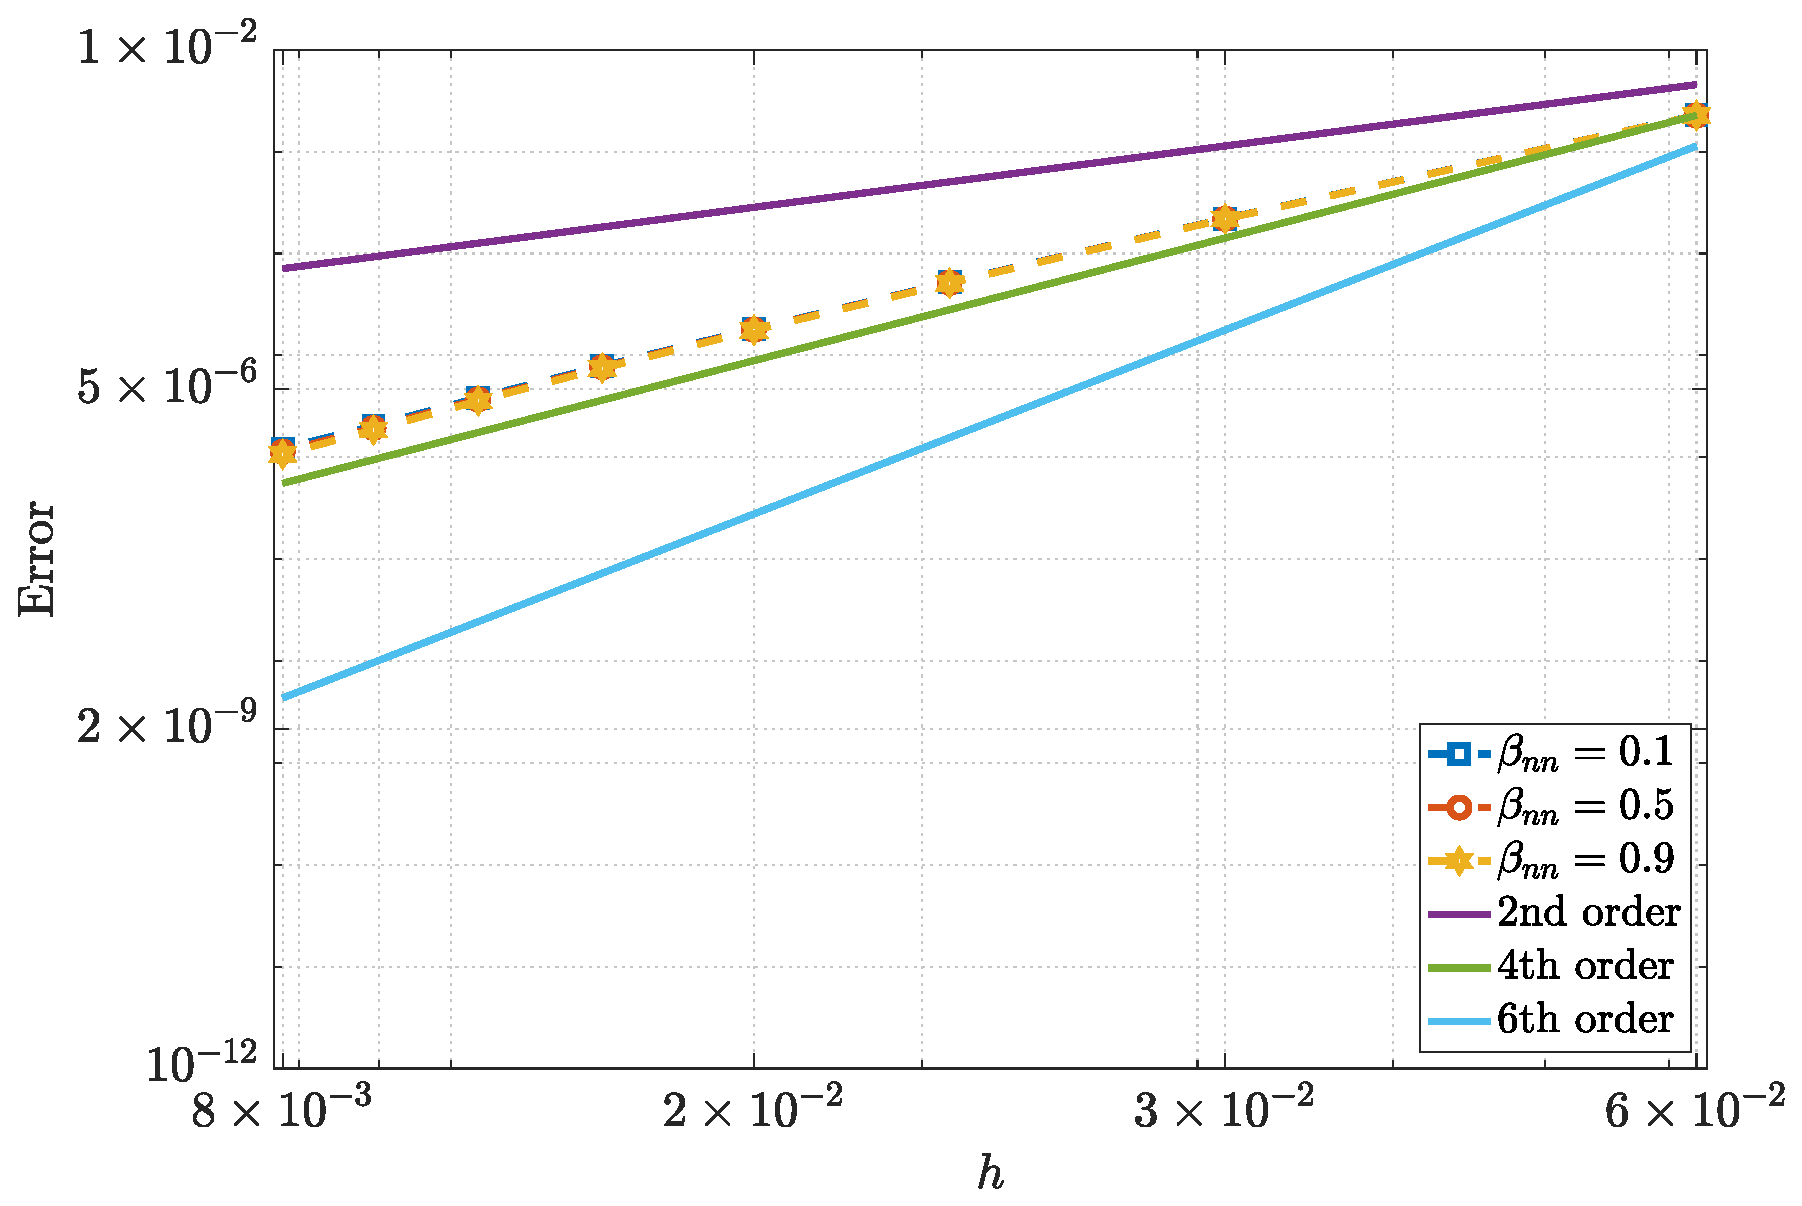
\includegraphics[width=\textwidth]{NormErr_2nd_Re_100_Wi_1_epsilon_0_xi_0_alphaG_0.5_Dt_1e-06_at_0.05_tipsim_1_MMS_12_Wz.eps}
        \caption{$||\omega_{z} - \widetilde{\omega_{z}}||_{2}$}
        \label{error_wz_2nd_Case1_giesekus_alphaG_0.5}
    \end{subfigure}
    \qquad
    \begin{subfigure}[b]{.46\textwidth}
        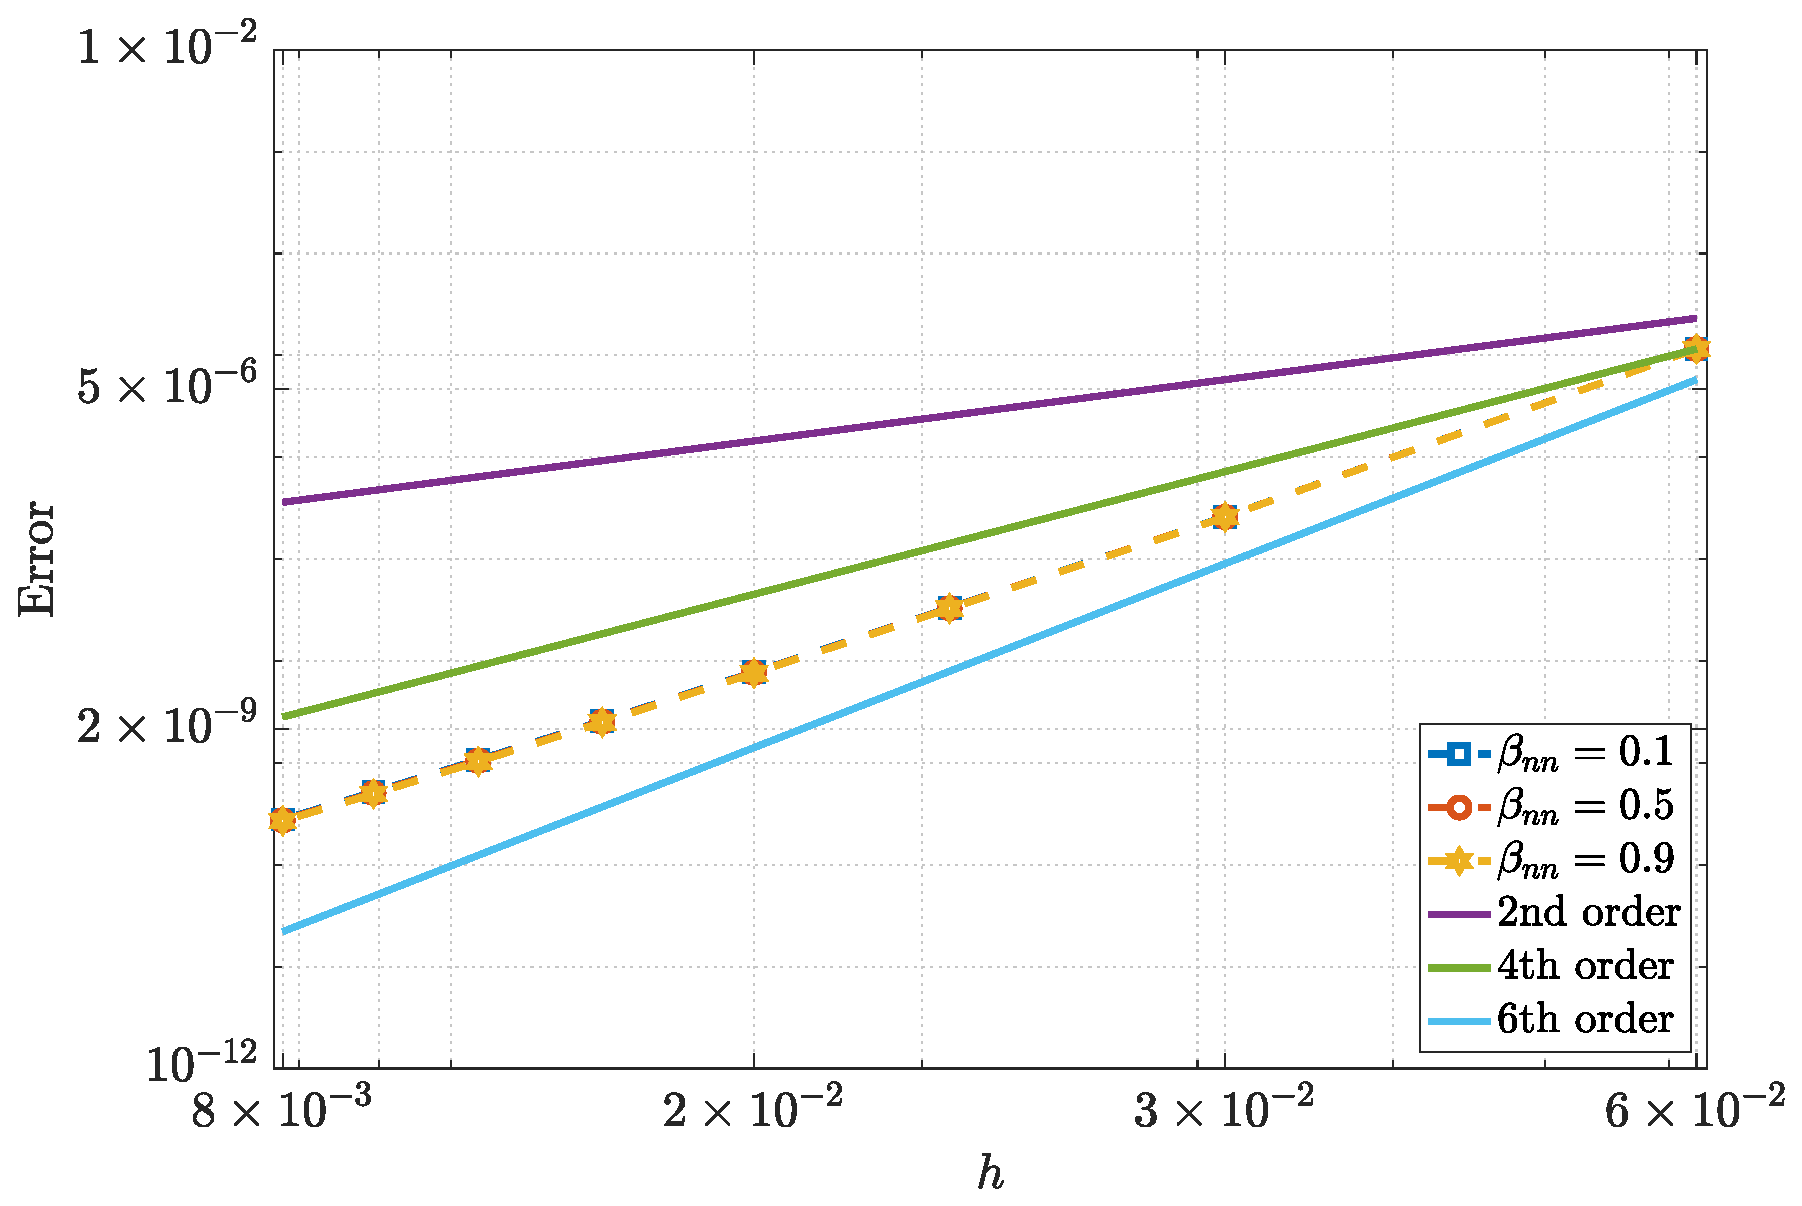
\includegraphics[width=\textwidth]{NormErr_2nd_Re_100_Wi_1_epsilon_0_xi_0_alphaG_0.5_Dt_1e-06_at_0.05_tipsim_1_MMS_12_Psi.eps}
        \caption{$||\Psi - \widetilde{\Psi}||_{2}$}
        \label{error_psi_2nd_Case1_oldorydbgiesekus_alphaG_0.5}
    \end{subfigure}
    \vspace{0.02cm}
    \caption{Error for the velocity field $({u},{v})$, vorticity $({\omega_{z}})$, and stream function$({\Psi})$, with $\operatorname{Re}=100$, $Wi=1$ and $\alpha_G=0.5$ for the Giesekus viscoelastic fluid flow using different solvent viscosity ratios ($\beta_{nn}$) and grid sizes ($\Delta x, \Delta y$).\label{GEerror051}}
\end{figure}

In Figure~\ref{GEerror052} we show the error plots for the polymeric tensor
components ($T_{xx},~T_{xy},~T_{yy}$) using different grid sizes ($\Delta x,
\Delta y$), for the viscoelastic Giesekus fluid flow at
$\operatorname{Re}=100$, $Wi=1$ and $\alpha_G=0.5$.

\begin{figure}[H]
    \centering  
    \begin{subfigure}[b]{.46\textwidth}
        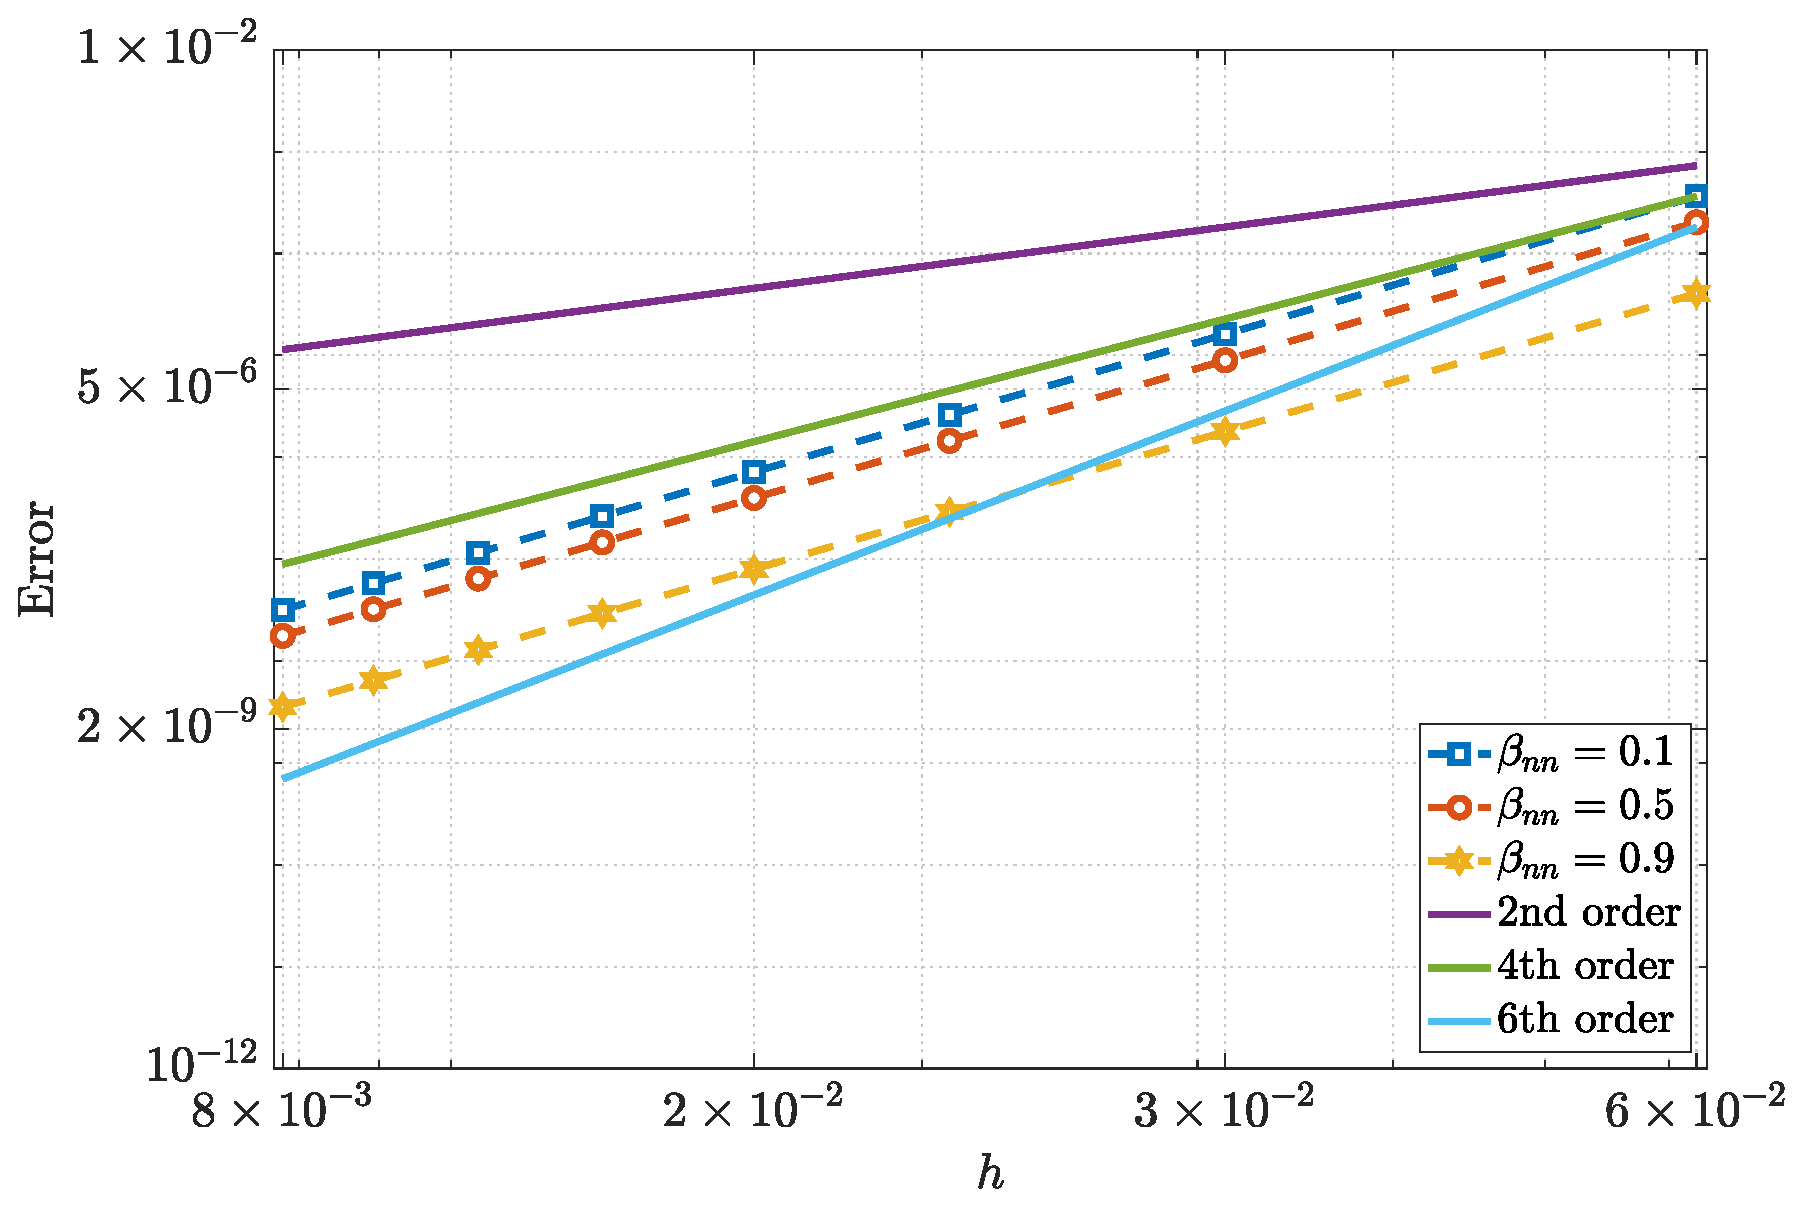
\includegraphics[width=\textwidth]{NormErr_2nd_Re_100_Wi_1_epsilon_0_xi_0_alphaG_0.5_Dt_1e-06_at_0.05_tipsim_1_MMS_12_Txx.eps}
        \caption{$||T_{xx} - \overline{T}_{xx}||_{2}$}
        \label{error_txx_2nd_Case1_giesekus_alphaG_0.5}
    \end{subfigure}
    \vspace{0.2cm}
    \qquad
    \begin{subfigure}[b]{.46\textwidth}
        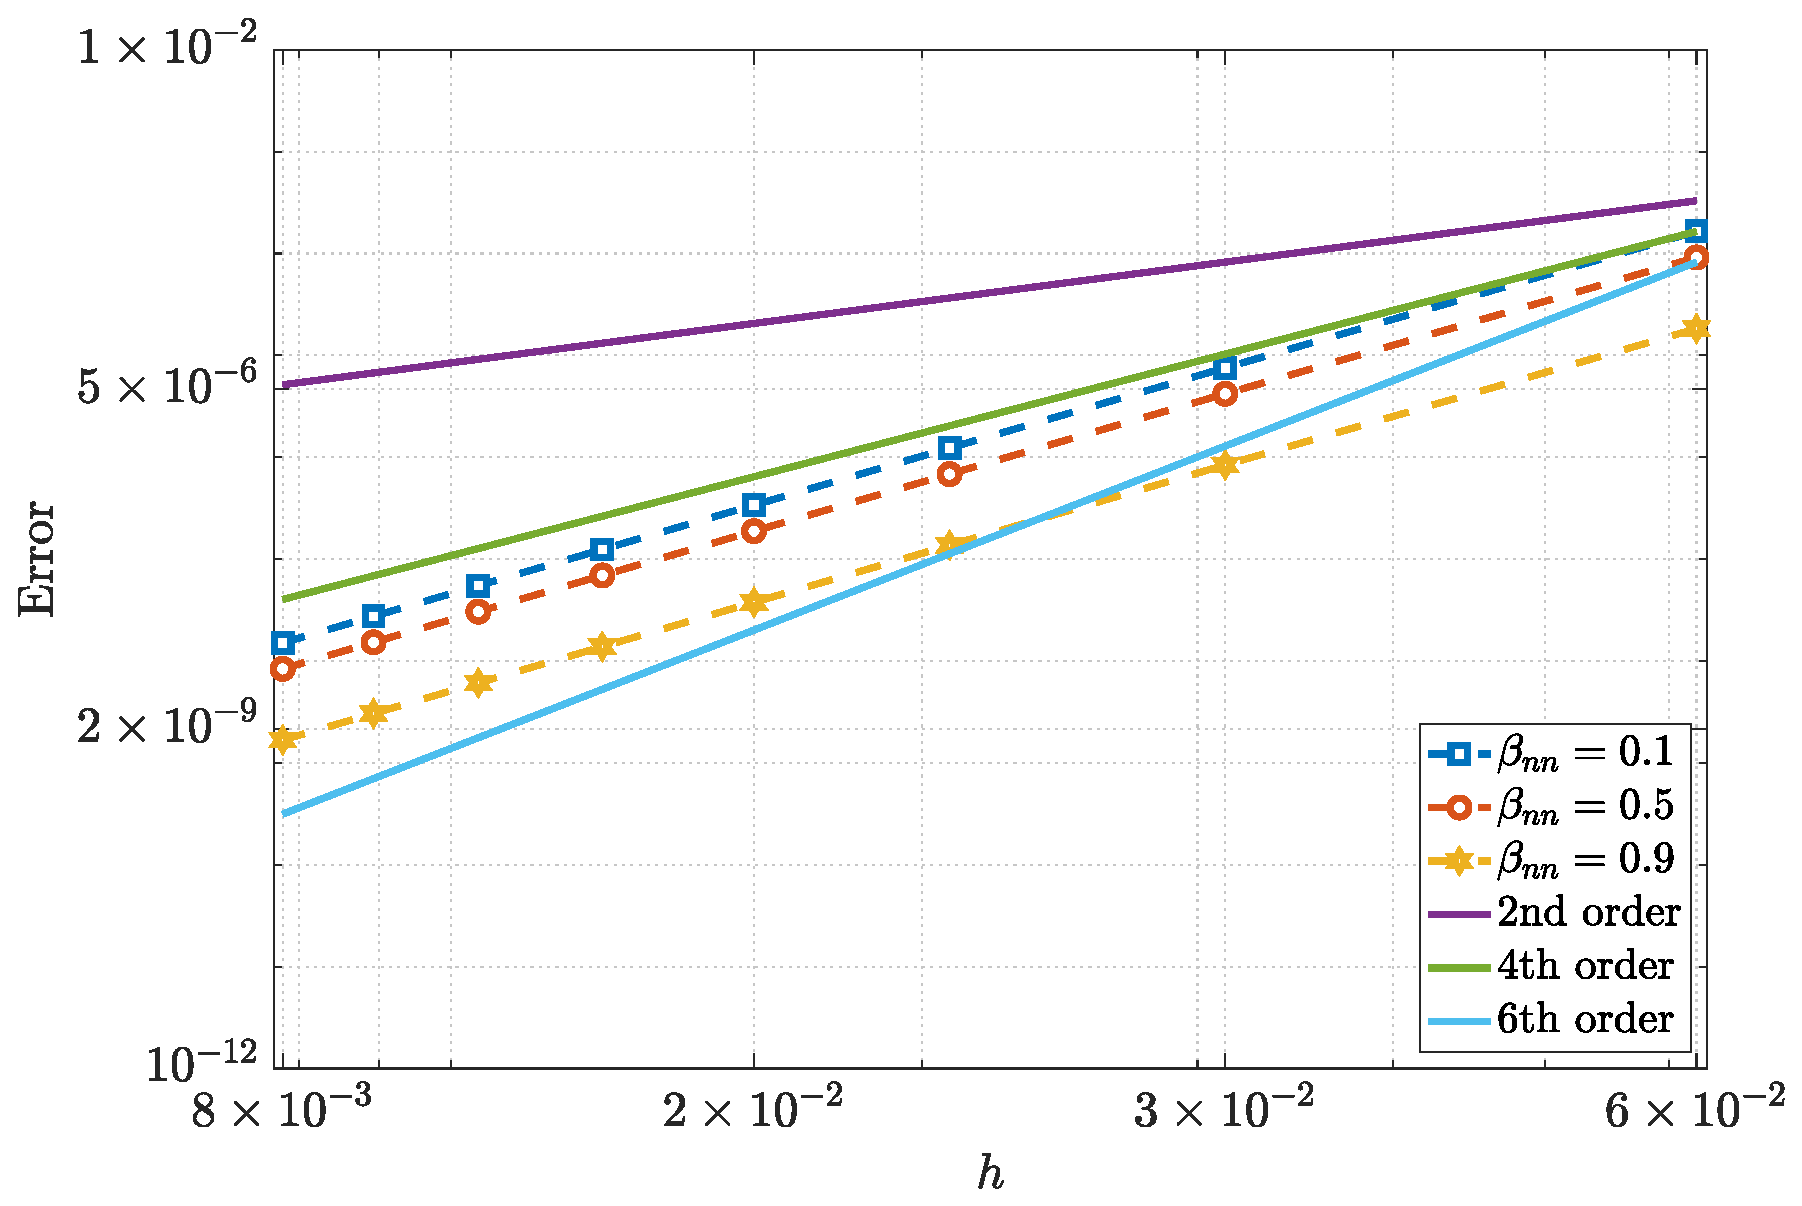
\includegraphics[width=\textwidth]{NormErr_2nd_Re_100_Wi_1_epsilon_0_xi_0_alphaG_0.5_Dt_1e-06_at_0.05_tipsim_1_MMS_12_Txy.eps}
        \caption{$||T_{xy} - \overline{T}_{xy}||_{2}$}
        \label{error_txy_2nd_Case1_giesekus_alphaG_0.5}
    \end{subfigure}
    \qquad
    \begin{subfigure}[b]{.46\textwidth}
        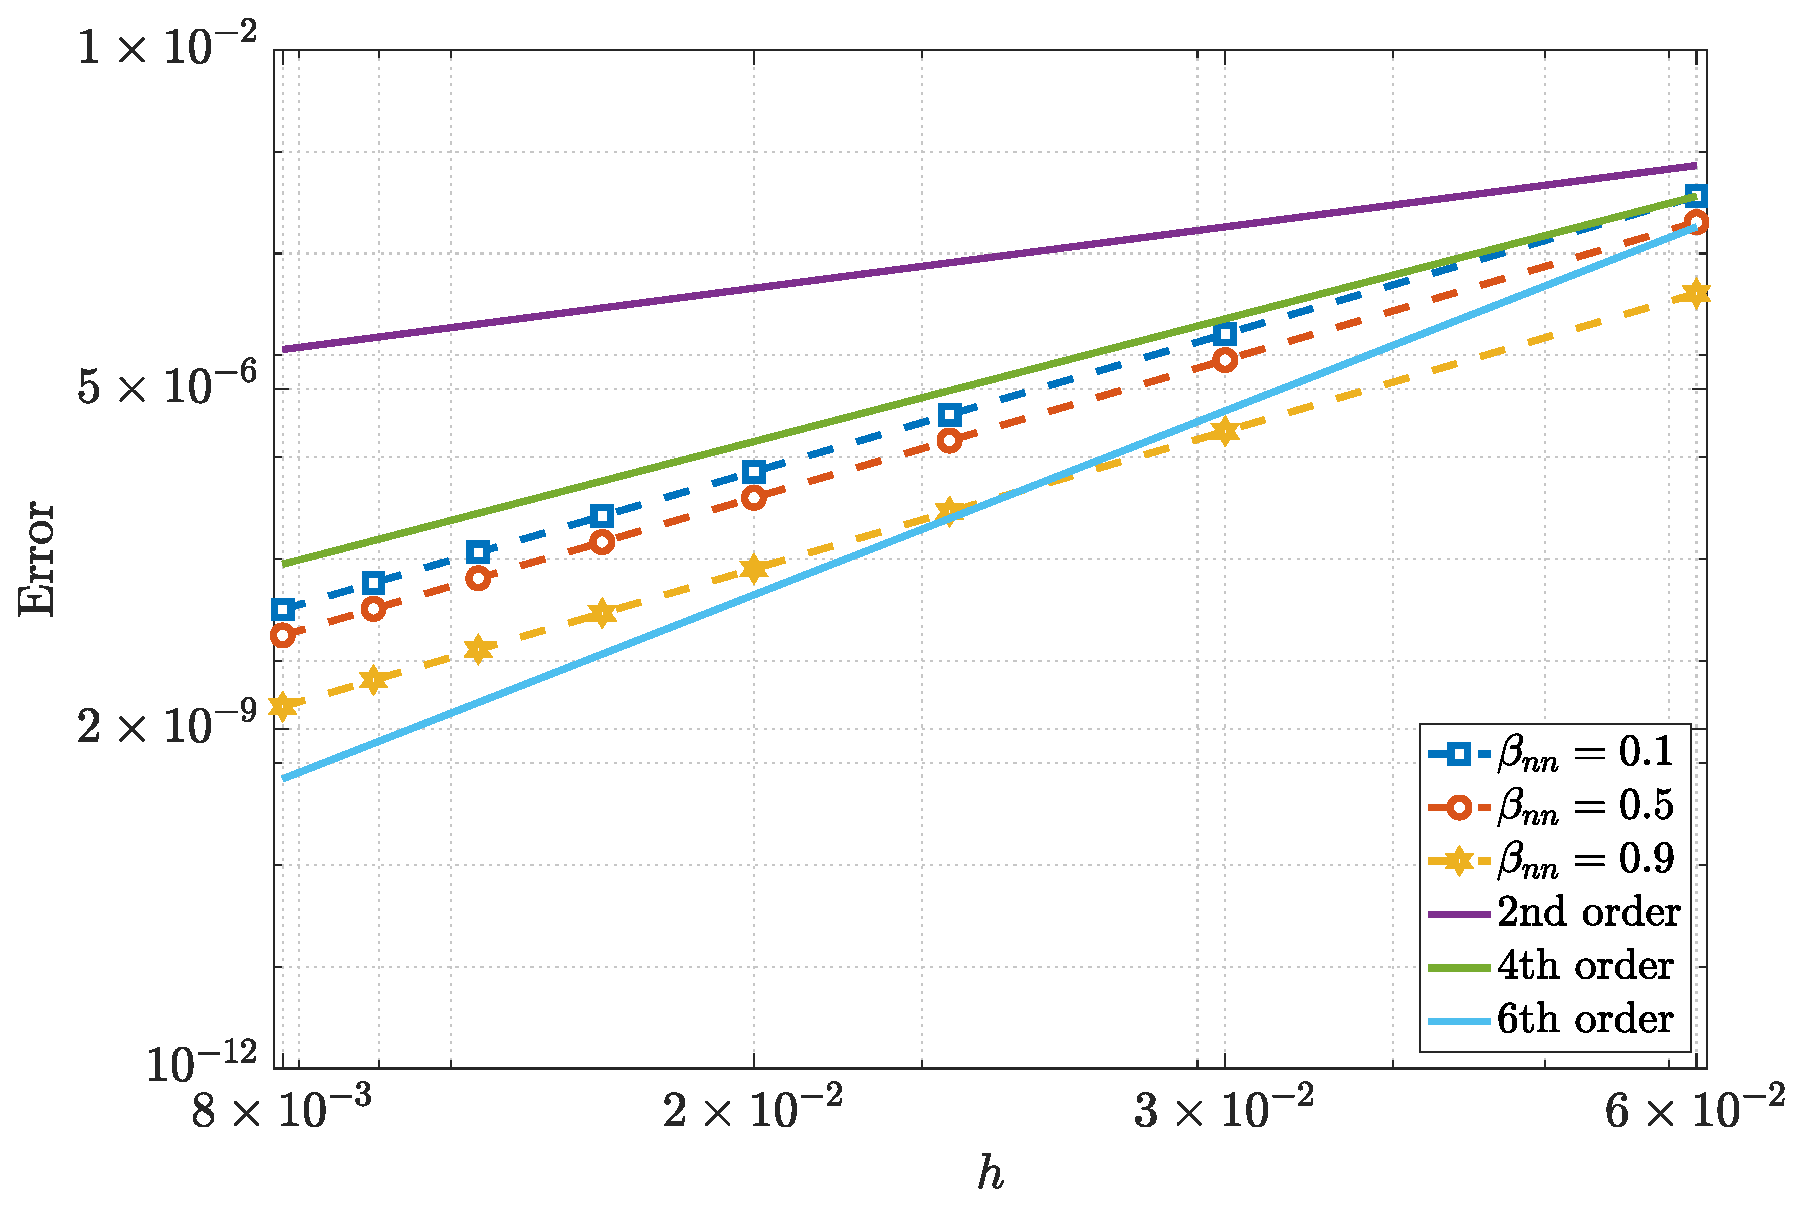
\includegraphics[width=\textwidth]{NormErr_2nd_Re_100_Wi_1_epsilon_0_xi_0_alphaG_0.5_Dt_1e-06_at_0.05_tipsim_1_MMS_12_Tyy.eps}
        \caption{$||T_{yy} - \overline{T}_{yy}||_{2}$}
        \label{error_tyy_2nd_Case1_giesekus_alphaG_0.5}
    \end{subfigure}
    \vspace{0.02cm}
    \caption{Error for the polymeric tensor components ($T_{xx},~T_{xy},~T_{yy}$), with $\operatorname{Re}=100,$ $Wi=1$ and $\alpha_{G} = 0.5$ for the Giesekus viscoelastic fluid flow using different solvent viscosity ratios ($\beta_{nn}$) and grid sizes ($\Delta x, \Delta y$).\label{GEerror052}}
\end{figure}

In the simulations with $\alpha_G = 0.5$, presented in Figures~\ref{GEerror051}
and \ref{GEerror052}, a similarity is observed in the results compared to those
obtained with $\alpha_G = 0.1$. The convergence order remains consistent, close
to $4.5$ for all variables studied, including polymeric tensor components and
vorticity. This indicates that the {\color{red} adopted high-order numerical code is stable
and accurate in a wide range of $\alpha_G$ values, making it applicable under
various flow conditions.}

\begin{center}
\begin{table}[H]
\caption{Numerical errors and convergence order calculation for vorticity ($\omega_{z}$), using \mbox{$Wi=1$}, $Re=\{1,100,400,1000\}$, $\beta_{nn}=\{0.1,0.5,0.9,1.0\}$ and $\alpha_G = 0.5$, for the Giesekus viscoelastic fluid flow.\label{tab_GiesekusWzalphaG05Resumida}}
\scriptsize{
    \begin{tabular*}{\textwidth}{@{\extracolsep\fill}cccccccccc@{}}
    \hline
    \multirow{2}{*}{$\operatorname{Re}$} & \multirow{2}{*}{Mesh} & \multicolumn{2}{c}{$\beta_{nn}=0.1$}  & \multicolumn{2}{c}{$\beta_{nn}=0.5$}  & \multicolumn{2}{c}{$\beta_{nn}=0.9$}  & \multicolumn{2}{c}{$\beta_{nn}=1.0$}\\ %\cline{3-10}
     & & Error & Order & Error & Order & Error & Order & Error & Order \\
    \hline
    \multirow{7}{*}{1.00} & $17\times 17$ & 2.23e-03 & --- & 2.08e-03 & --- & 1.96e-03 & --- & 1.93e-03 & --- \\
    & $33\times 33$ & 2.02e-04 & 3.47 & 1.51e-04 & 3.79 & 1.23e-04 & 4.00 & 1.18e-04 & 4.03 \\
    & $49\times 49$ & 4.26e-05 & 3.84 & 2.50e-05 & 4.44 & 1.92e-05 & 4.57 & 1.84e-05 & 4.58 \\
    & $65\times 65$ & 1.28e-05 & 4.17 & 6.43e-06 & 4.71 & 5.05e-06 & 4.65 & 4.85e-06 & 4.63 \\
    & $81\times 81$ & 4.68e-06 & 4.52 & 2.23e-06 & 4.74 & 1.79e-06 & 4.63 & 1.73e-06 & 4.61 \\
    & $97\times 97$ & 1.92e-06 & 4.90 & 9.34e-07 & 4.78 & 7.68e-07 & 4.65 & 7.45e-07 & 4.63 \\
    & $113\times 113$ & 8.58e-07 & 5.21 & 4.47e-07 & 4.77 & 3.80e-07 & 4.57 & 3.71e-07 & 4.52 \\
    & $129\times 129$ & 4.34e-07 & 5.10 & 2.59e-07 & 4.11 & 2.30e-07 & 3.76 & 2.26e-07 & 3.71 \\
    \hline\hline
    \multirow{7}{*}{100.00} & $17\times 17$ & 2.27e-03 & --- & 2.27e-03 & --- & 2.26e-03 & --- & 2.26e-03 & --- \\
    & $33\times 33$ & 2.20e-04 & 3.37 & 2.19e-04 & 3.37 & 2.18e-04 & 3.37 & 2.18e-04 & 3.37 \\
    & $49\times 49$ & 5.20e-05 & 3.56 & 5.15e-05 & 3.57 & 5.11e-05 & 3.58 & 5.10e-05 & 3.59 \\
    & $65\times 65$ & 1.82e-05 & 3.66 & 1.79e-05 & 3.68 & 1.76e-05 & 3.70 & 1.75e-05 & 3.71 \\
    & $81\times 81$ & 7.84e-06 & 3.76 & 7.65e-06 & 3.80 & 7.47e-06 & 3.84 & 7.43e-06 & 3.85 \\
    & $97\times 97$ & 3.83e-06 & 3.93 & 3.70e-06 & 3.99 & 3.57e-06 & 4.05 & 3.54e-06 & 4.06 \\
    & $113\times 113$ & 2.04e-06 & 4.10 & 1.94e-06 & 4.19 & 1.85e-06 & 4.27 & 1.83e-06 & 4.29 \\
    & $129\times 129$ & 1.21e-06 & 3.89 & 1.13e-06 & 4.02 & 1.07e-06 & 4.13 & 1.05e-06 & 4.16 \\
    \hline\hline
    \multirow{7}{*}{400.00} & $17\times 17$ & 2.27e-03 & --- & 2.27e-03 & --- & 2.27e-03 & --- & 2.27e-03 & --- \\
    & $33\times 33$ & 2.20e-04 & 3.37 & 2.20e-04 & 3.37 & 2.20e-04 & 3.37 & 2.20e-04 & 3.37 \\
    & $49\times 49$ & 5.21e-05 & 3.56 & 5.19e-05 & 3.56 & 5.18e-05 & 3.56 & 5.18e-05 & 3.56 \\
    & $65\times 65$ & 1.82e-05 & 3.65 & 1.81e-05 & 3.66 & 1.81e-05 & 3.66 & 1.81e-05 & 3.66 \\
    & $81\times 81$ & 7.88e-06 & 3.75 & 7.83e-06 & 3.76 & 7.79e-06 & 3.77 & 7.78e-06 & 3.77 \\
    & $97\times 97$ & 3.86e-06 & 3.92 & 3.82e-06 & 3.93 & 3.80e-06 & 3.94 & 3.79e-06 & 3.95 \\
    & $113\times 113$ & 2.05e-06 & 4.09 & 2.03e-06 & 4.11 & 2.01e-06 & 4.12 & 2.01e-06 & 4.13 \\
    & $129\times 129$ & 1.23e-06 & 3.86 & 1.21e-06 & 3.89 & 1.19e-06 & 3.92 & 1.19e-06 & 3.93 \\
    \hline\hline
    \multirow{7}{*}{1000.00} & $17\times 17$ & 2.27e-03 & --- & 2.27e-03 & --- & 2.27e-03 & --- & 2.27e-03 & --- \\
    & $33\times 33$ & 2.20e-04 & 3.37 & 2.20e-04 & 3.37 & 2.20e-04 & 3.37 & 2.20e-04 & 3.37 \\
    & $49\times 49$ & 5.21e-05 & 3.56 & 5.20e-05 & 3.56 & 5.20e-05 & 3.56 & 5.20e-05 & 3.56 \\
    & $65\times 65$ & 1.82e-05 & 3.65 & 1.82e-05 & 3.65 & 1.82e-05 & 3.65 & 1.82e-05 & 3.65 \\
    & $81\times 81$ & 7.89e-06 & 3.75 & 7.87e-06 & 3.76 & 7.86e-06 & 3.76 & 7.85e-06 & 3.76 \\
    & $97\times 97$ & 3.86e-06 & 3.92 & 3.85e-06 & 3.92 & 3.84e-06 & 3.92 & 3.84e-06 & 3.92 \\
    & $113\times 113$ & 2.06e-06 & 4.08 & 2.05e-06 & 4.09 & 2.04e-06 & 4.09 & 2.04e-06 & 4.09 \\
    & $129\times 129$ & 1.23e-06 & 3.85 & 1.22e-06 & 3.87 & 1.22e-06 & 3.87 & 1.22e-06 & 3.88 \\
    \hline
    \end{tabular*}
}
\end{table}
\end{center}

\begin{center}
\begin{table}[H]
\caption{Numerical errors and convergence order calculation for the polymeric tensor component $T_{yy}$, using \mbox{$Wi=1$}, $Re=\{1,100,400,1000\}$, $\beta_{nn}=\{0.1,0.5,0.9,1.0\}$ and \mbox{$\alpha_G = 0.5$}, for the Giesekus viscoelastic fluid flow.\label{tab_GiesekusTyyalphaG05Resumida}}
\scriptsize{
    \begin{tabular*}{\textwidth}{@{\extracolsep\fill}cccccccccc@{}}
    \hline
    \multirow{2}{*}{$\operatorname{Re}$} & \multirow{2}{*}{Mesh} & \multicolumn{2}{c}{$\beta_{nn}=0.1$}  & \multicolumn{2}{c}{$\beta_{nn}=0.5$}  & \multicolumn{2}{c}{$\beta_{nn}=0.9$}  & \multicolumn{2}{c}{$\beta_{nn}=1.0$}\\ %\cline{3-10}
     & & Error & Order & Error & Order & Error & Order & Error & Order \\
    \hline
    \multirow{7}{*}{1.00} & $17\times 17$ & 3.90e-04 & --- & 2.17e-04 & --- & 4.33e-05 & --- & 4.33e-18 & --- \\
    & $33\times 33$ & 1.70e-05 & 4.52 & 9.43e-06 & 4.52 & 1.89e-06 & 4.52 & 1.88e-19 & 4.52 \\
    & $49\times 49$ & 2.73e-06 & 4.50 & 1.52e-06 & 4.51 & 3.03e-07 & 4.51 & 3.03e-20 & 4.51 \\
    & $65\times 65$ & 7.48e-07 & 4.50 & 4.15e-07 & 4.50 & 8.31e-08 & 4.50 & 8.30e-21 & 4.50 \\
    & $81\times 81$ & 2.74e-07 & 4.50 & 1.52e-07 & 4.50 & 3.04e-08 & 4.50 & 3.04e-21 & 4.50 \\
    & $97\times 97$ & 1.21e-07 & 4.50 & 6.70e-08 & 4.50 & 1.34e-08 & 4.50 & 1.34e-21 & 4.50 \\
    & $113\times 113$ & 6.03e-08 & 4.50 & 3.35e-08 & 4.50 & 6.70e-09 & 4.50 & 6.69e-22 & 4.50 \\
    & $129\times 129$ & 3.31e-08 & 4.50 & 1.84e-08 & 4.50 & 3.67e-09 & 4.50 & 3.67e-22 & 4.50 \\
    \hline\hline
    \multirow{7}{*}{100.00} & $17\times 17$ & 3.65e-04 & --- & 2.03e-04 & --- & 4.06e-05 & --- & 4.05e-18 & --- \\
    & $33\times 33$ & 1.62e-05 & 4.49 & 9.00e-06 & 4.49 & 1.80e-06 & 4.49 & 1.80e-19 & 4.49 \\
    & $49\times 49$ & 2.62e-06 & 4.49 & 1.46e-06 & 4.49 & 2.92e-07 & 4.49 & 2.91e-20 & 4.49 \\
    & $65\times 65$ & 7.21e-07 & 4.49 & 4.01e-07 & 4.49 & 8.02e-08 & 4.49 & 8.01e-21 & 4.49 \\
    & $81\times 81$ & 2.65e-07 & 4.49 & 1.47e-07 & 4.49 & 2.94e-08 & 4.49 & 2.94e-21 & 4.49 \\
    & $97\times 97$ & 1.17e-07 & 4.49 & 6.49e-08 & 4.49 & 1.30e-08 & 4.49 & 1.30e-21 & 4.49 \\
    & $113\times 113$ & 5.84e-08 & 4.49 & 3.24e-08 & 4.49 & 6.49e-09 & 4.49 & 6.48e-22 & 4.49 \\
    & $129\times 129$ & 3.21e-08 & 4.49 & 1.78e-08 & 4.49 & 3.56e-09 & 4.49 & 3.56e-22 & 4.49 \\
    \hline\hline
    \multirow{7}{*}{400.00} & $17\times 17$ & 3.12e-04 & --- & 1.74e-04 & --- & 3.47e-05 & --- & 3.47e-18 & --- \\
    & $33\times 33$ & 1.45e-05 & 4.43 & 8.07e-06 & 4.43 & 1.61e-06 & 4.43 & 1.61e-19 & 4.43 \\
    & $49\times 49$ & 2.40e-06 & 4.44 & 1.33e-06 & 4.44 & 2.66e-07 & 4.44 & 2.66e-20 & 4.44 \\
    & $65\times 65$ & 6.65e-07 & 4.46 & 3.69e-07 & 4.46 & 7.38e-08 & 4.46 & 7.38e-21 & 4.46 \\
    & $81\times 81$ & 2.45e-07 & 4.47 & 1.36e-07 & 4.47 & 2.73e-08 & 4.47 & 2.72e-21 & 4.47 \\
    & $97\times 97$ & 1.09e-07 & 4.47 & 6.03e-08 & 4.47 & 1.21e-08 & 4.47 & 1.20e-21 & 4.47 \\
    & $113\times 113$ & 5.44e-08 & 4.48 & 3.02e-08 & 4.48 & 6.05e-09 & 4.48 & 6.04e-22 & 4.48 \\
    & $129\times 129$ & 2.99e-08 & 4.48 & 1.66e-08 & 4.48 & 3.32e-09 & 4.48 & 3.32e-22 & 4.48 \\
    \hline\hline
    \multirow{7}{*}{1000.00} & $17\times 17$ & 2.58e-04 & --- & 1.43e-04 & --- & 2.87e-05 & --- & 2.87e-18 & --- \\
    & $33\times 33$ & 1.28e-05 & 4.34 & 7.11e-06 & 4.34 & 1.42e-06 & 4.34 & 1.42e-19 & 4.34 \\
    & $49\times 49$ & 2.16e-06 & 4.38 & 1.20e-06 & 4.38 & 2.40e-07 & 4.38 & 2.40e-20 & 4.38 \\
    & $65\times 65$ & 6.08e-07 & 4.41 & 3.38e-07 & 4.41 & 6.75e-08 & 4.41 & 6.75e-21 & 4.41 \\
    & $81\times 81$ & 2.26e-07 & 4.43 & 1.26e-07 & 4.43 & 2.51e-08 & 4.43 & 2.51e-21 & 4.43 \\
    & $97\times 97$ & 1.01e-07 & 4.44 & 5.59e-08 & 4.44 & 1.12e-08 & 4.44 & 1.12e-21 & 4.44 \\
    & $113\times 113$ & 5.06e-08 & 4.45 & 2.81e-08 & 4.45 & 5.63e-09 & 4.45 & 5.62e-22 & 4.45 \\
    & $129\times 129$ & 2.79e-08 & 4.46 & 1.55e-08 & 4.46 & 3.10e-09 & 4.46 & 3.10e-22 & 4.46 \\
    \hline
    \end{tabular*}
}
\end{table}
\end{center}

Similarly, Tables~\ref{tab_GiesekusWzalphaG05Resumida} and
\ref{tab_GiesekusTyyalphaG05Resumida} present the error results and the
convergence order for $\omega_{z}$ and $T_{yy}$, respectively, when $\alpha_G =
0.5$. It is observed that, regardless of the value of $\alpha_G$, the results
maintain high accuracy and a stable convergence order. This behaviour
highlights the Giesekus {\color{red} constitutive model's capability to accurately simulate
different conditions of viscosity and elasticity, ensuring that the numerical
method applies to a wide range of viscoelastic problems.}

Figures \ref{fig_slice_Solution_uvwzpsi_Giesekus_x075} and
\ref{fig_slice_Solution_uvwzpsi_Giesekus_x025} display profiles of the velocity
field components $(u, v)$, vorticity $(\omega_z)$, and stream function $(\Psi)$
along the lines $x=0.25$ and $y=0.75$, respectively, for the Giesekus
constitutive model with $\alpha_G = 0.5$, under the conditions of
$\operatorname{Re}=1000$, $Wi=1$ and different solvent viscosity ratios. In
this context, the continuous lines represent the manufactured solutions, while
the markers correspond to the numerical solutions, both computed under the same
parameters. The numerical results reveal the distribution of normal and shear
stresses within the flow domain, demonstrating a high level of agreement with
the expected behaviour. It is evident that, as $\beta_{nn}$ approaches 1, the
values of $(T_{xx}, T_{xy}, T_{yy})$ converge to the null tensor, indicating a
gradual transition from viscoelastic behaviour to a Newtonian regime. This
behaviour reflects a significant reduction in elastic effects and the dominance
of viscous forces, thereby confirming the robustness and the accuracy of the
numerical method adopted.

\begin{figure}[H]
    \centering
    \begin{subfigure}[b]{.46\textwidth}
        \includegraphics[width=\textwidth]{Slice_x_Tog_Numerical_NormErr_2nd_Betann_1_Re_1000_Wi_1_epsilon_0_xi_0_alphaG_0.5_Dt_1e-06_at_0.05_tipsim_1_MMS_12_x0.75y0.75_U.eps}
        \caption{Profile at $x=0.75$ for the velocity field component $(u)$}
        \label{fig_slice_y_u_2nd_Case1_giesekus_x075}
    \end{subfigure}
    \vspace{0.2cm}
    \qquad
    \begin{subfigure}[b]{.46\textwidth}
        \includegraphics[width=\textwidth]{Slice_x_Tog_Numerical_NormErr_2nd_Betann_1_Re_1000_Wi_1_epsilon_0_xi_0_alphaG_0.5_Dt_1e-06_at_0.05_tipsim_1_MMS_12_x0.75y0.75_V.eps}
        \caption{Profile at $x=0.75$ for the velocity field component $(v)$}
        \label{fig_slice_y_v_2nd_Case1_giesekus_x075}
    \end{subfigure}
    \begin{subfigure}[b]{.46\textwidth}
        \includegraphics[width=\textwidth]{Slice_x_Tog_Numerical_NormErr_2nd_Betann_1_Re_1000_Wi_1_epsilon_0_xi_0_alphaG_0.5_Dt_1e-06_at_0.05_tipsim_1_MMS_12_x0.75y0.75_Wz.eps}
        \caption{Profile at $x=0.75$ for the vorticity $(\omega_{z})$}
        \label{fig_slice_y_wz_2nd_Case1_giesekus_x075}
    \end{subfigure}
    \vspace{0.2cm}
    \qquad
    \begin{subfigure}[b]{.46\textwidth}
        \includegraphics[width=\textwidth]{Slice_x_Tog_Numerical_NormErr_2nd_Betann_1_Re_1000_Wi_1_epsilon_0_xi_0_alphaG_0.5_Dt_1e-06_at_0.05_tipsim_1_MMS_12_x0.75y0.75_Psi.eps}
        \caption{Profile at $x=0.75$ for the stream function $(\Psi)$}
        \label{fig_slice_y_psi_2nd_Case1_giesekus_x075}
    \end{subfigure}
    \vspace{0.02cm}
    \caption{Profiles for the velocity field $(u,v)$, vorticity $(\omega_{z})$, and stream function $(\Psi)$, using $\operatorname{Re}=1000, $ $Wi=1$ and $\alpha_{G} = 0.5$, for the Giesekus viscoelastic fluid flow, where the continuous lines represent the manufactured solutions, and the markers correspond to the numerical solutions, both computed under the same parameters.\label{fig_slice_Solution_uvwzpsi_Giesekus_x075}}
\end{figure}

\begin{figure}[H]
    \centering
    \begin{subfigure}[b]{.46\textwidth}
        \includegraphics[width=\textwidth]{Slice_y_Tog_Numerical_NormErr_2nd_Betann_1_Re_1000_Wi_1_epsilon_0_xi_0_alphaG_0.5_Dt_1e-06_at_0.05_tipsim_1_MMS_12_x0.25y0.25_U.eps}
        \caption{Profile at $y=0.25$ for the velocity field component $(u)$}
        \label{fig_slice_y_u_2nd_Case1_giesekus_y025}
    \end{subfigure}
    \vspace{0.2cm}
    \qquad
    \begin{subfigure}[b]{.46\textwidth}
        \includegraphics[width=\textwidth]{Slice_y_Tog_Numerical_NormErr_2nd_Betann_1_Re_1000_Wi_1_epsilon_0_xi_0_alphaG_0.5_Dt_1e-06_at_0.05_tipsim_1_MMS_12_x0.25y0.25_V.eps}
        \caption{Profile at $y=0.25$ for the velocity field component $(v)$}
        \label{fig_slice_y_v_2nd_Case1_giesekus_y025}
    \end{subfigure}
    \begin{subfigure}[b]{.46\textwidth}
        \includegraphics[width=\textwidth]{Slice_y_Tog_Numerical_NormErr_2nd_Betann_1_Re_1000_Wi_1_epsilon_0_xi_0_alphaG_0.5_Dt_1e-06_at_0.05_tipsim_1_MMS_12_x0.25y0.25_Wz.eps}
        \caption{Profile at $y=0.25$ for the vorticity $(\omega_{z})$}
        \label{fig_slice_y_wz_2nd_Case1_giesekus_y025}
    \end{subfigure}
    \vspace{0.2cm}
    \qquad
    \begin{subfigure}[b]{.46\textwidth}
        \includegraphics[width=\textwidth]{Slice_y_Tog_Numerical_NormErr_2nd_Betann_1_Re_1000_Wi_1_epsilon_0_xi_0_alphaG_0.5_Dt_1e-06_at_0.05_tipsim_1_MMS_12_x0.25y0.25_Psi.eps}
        \caption{Profile at $y=0.25$ for the stream function $(\Psi)$}
        \label{fig_slice_y_psi_2nd_Case1_giesekus_y025}
    \end{subfigure}
    \vspace{0.02cm}
    \caption{Profiles for the velocity field $(u,v)$, vorticity $(\omega_{z})$ and stream function $(\Psi)$, using $\operatorname{Re}=1000,$ $Wi=1$ and $\alpha_{G} = 0.5$, for the Giesekus viscoelastic fluid flow, where the continuous lines represent the manufactured solutions, and the markers correspond to the numerical solutions, both computed under the same parameters.\label{fig_slice_Solution_uvwzpsi_Giesekus_x025}}
\end{figure}

Figures \ref{fig_slice_Solution_txxxyyy_Giesekus_x075} and
\ref{fig_slice_Solution_txxxyyy_Giesekus_y025} present slices for the
components of the extra stress tensor $(T_{xx}, T_{xy}, T_{yy})$, providing
insights into the distribution of normal and shear stresses within the flow
domain along the lines $x=0.75$ and $y=0.25$, for the Giesekus constitutive
model with $\alpha_G = 0.5$, under the conditions $\operatorname{Re}=1000$ and
$Wi=1$, where the continuous lines represent the manufactured solutions, and
the markers correspond to the numerical solutions, both computed under the same
parameters.

\begin{figure}[H]
    \centering
    \begin{subfigure}[b]{.46\textwidth}
        \includegraphics[width=\textwidth]{Slice_x_Tog_Numerical_NormErr_2nd_Betann_1_Re_1000_Wi_1_epsilon_0_xi_0_alphaG_0.5_Dt_1e-06_at_0.05_tipsim_1_MMS_12_x0.75y0.75_Txx.eps}
        \caption{Slice at $x=0.75$ for the extra-stress component $T_{xx}$}
        \label{fig_slice_y_txx_2nd_Case1_giesekus_x075}
    \end{subfigure}
    \vspace{0.2cm}
    \qquad
    \begin{subfigure}[b]{.46\textwidth}
        \includegraphics[width=\textwidth]{Slice_x_Tog_Numerical_NormErr_2nd_Betann_1_Re_1000_Wi_1_epsilon_0_xi_0_alphaG_0.5_Dt_1e-06_at_0.05_tipsim_1_MMS_12_x0.75y0.75_Txy.eps}
        \caption{Slice at $x=0.75$ for the extra-stress component $T_{xy}$}
        \label{fig_slice_y_txy_2nd_Case1_giesekus_x075}
    \end{subfigure}
    \begin{subfigure}[b]{.46\textwidth}
        \includegraphics[width=\textwidth]{Slice_x_Tog_Numerical_NormErr_2nd_Betann_1_Re_1000_Wi_1_epsilon_0_xi_0_alphaG_0.5_Dt_1e-06_at_0.05_tipsim_1_MMS_12_x0.75y0.75_Tyy.eps}
        \caption{Slice at $x=0.75$ for the extra-stress component $T_{yy}$}
        \label{fig_slice_y_tyy_2nd_Case1_giesekus_x075}
    \end{subfigure}
    \vspace{0.02cm}
    \caption{Profiles for the polymeric tensor components ($T_{xx},~T_{xy},~T_{yy}$) at $x=0.75$, using $\operatorname{Re}=1000,$ $Wi=1$ and $\alpha_{G} = 0.5$, for the Giesekus viscoelastic fluid flow, where the continuous lines represent the manufactured solutions, and the markers correspond to the numerical solutions, both computed under the same parameters.\label{fig_slice_Solution_txxxyyy_Giesekus_x075}}
\end{figure}

\begin{figure}[H]
    \centering
    \begin{subfigure}[b]{.46\textwidth}
        \includegraphics[width=\textwidth]{Slice_y_Tog_Numerical_NormErr_2nd_Betann_1_Re_1000_Wi_1_epsilon_0_xi_0_alphaG_0.5_Dt_1e-06_at_0.05_tipsim_1_MMS_12_x0.25y0.25_Txx.eps}
        \caption{Profile at $y=0.25$ for the polymeric tensor component $T_{xx}$}
        \label{fig_slice_y_txx_2nd_Case1_giesekus_y025}
    \end{subfigure}
    \vspace{0.2cm}
    \qquad
    \begin{subfigure}[b]{.46\textwidth}
        \includegraphics[width=\textwidth]{Slice_y_Tog_Numerical_NormErr_2nd_Betann_1_Re_1000_Wi_1_epsilon_0_xi_0_alphaG_0.5_Dt_1e-06_at_0.05_tipsim_1_MMS_12_x0.25y0.25_Txy.eps}
        \caption{Profile at $y=0.25$ for the polymeric tensor component $T_{xy}$}
        \label{fig_slice_y_txy_2nd_Case1_giesekus_y025}
    \end{subfigure}
    \begin{subfigure}[b]{.46\textwidth}
        \includegraphics[width=\textwidth]{Slice_y_Tog_Numerical_NormErr_2nd_Betann_1_Re_1000_Wi_1_epsilon_0_xi_0_alphaG_0.5_Dt_1e-06_at_0.05_tipsim_1_MMS_12_x0.25y0.25_Tyy.eps}
        \caption{Profile at $y=0.25$ for the polymeric tensor component $T_{yy}$}
        \label{fig_slice_y_tyy_2nd_Case1_giesekus_y025}
    \end{subfigure}
    \vspace{0.02cm}
    \caption{Profiles for the polymeric tensor components ($T_{xx},~T_{xy},~T_{yy}$) at $y=0.25$, using $\operatorname{Re}=1000,$ $Wi=1$ and $\alpha_{G} = 0.5$, for the Giesekus viscoelastic fluid flow, where the continuous lines represent the manufactured solutions, and the markers correspond to the numerical solutions, both computed under the same parameters.\label{fig_slice_Solution_txxxyyy_Giesekus_y025}}
\end{figure}

In Figures \ref{fig_slice_Solution_txxxyyy_Giesekus_x075} and
\ref{fig_slice_Solution_txxxyyy_Giesekus_y025} we show profiles for the
polymeric tensor components $(T_{xx}, T_{xy}, T_{yy})$ for the Giesekus
constitutive model with $\alpha_G = 0.5$, providing information on the
distribution of normal and shear stresses within the flow domain along the
lines $x=0.75$ and $y=0.25$, respectively. Similarly to the results presented
for the Oldroyd-B constitutive model in Section \ref{subsec_oldroydb}, these
numerical results align well with the manufactured solutions. This agreement
confirms that the numerical solutions obtained by the employed methods follow
the expected behaviour, highlighting not only the accuracy of the methods but
also their robustness in reproducing complex viscoelastic flow solutions, in
both constitutive models used. As mentioned above, as the solvent viscosity
ratio $\beta_{nn}$ approaches 1, both manufactured and numerical solutions
along the lines $x=0.75$ and \mbox{$y=0.25$} show that the polymeric tensor
components $(T_{xx}, T_{xy}, T_{yy})$ tend to the null tensor. This behaviour
indicates a significant reduction in viscoelastic effects as the fluid
transitions to a Newtonian-like behaviour. 

{\color{red} The present code was also verified for higher Weissenberg numbers, for both
Oldroyd-B and Giesekus constitutive models. These results are shown in the \ref{Appendix_more_wi}.}


\section{Conclusions}\label{sec_Conclusions}

{\color{red} This study presents the application of the Method of Manufactured Solutions
(MMS) to verify numerical schemes for viscoelastic fluid flows, utilizing the
Oldroyd-B and Giesekus constitutive models. Simulations were conducted over a
range of Reynolds numbers (\( 1 \leq Re \leq 1000 \)), solvent viscosity ratios
(\( 0.1 \leq \beta_{nn} \leq 1 \)), and mobility factors (\( 0 \leq \alpha_G
\leq 0.5 \)), with varying Weissenberg numbers. Error analyses and convergence
rates confirmed the expected convergence order for all variables, including
velocity components, vorticity, streamfunction, and polymeric stress tensor
components, underscoring the robustness and accuracy of the employed high-order
numerical schemes.

For the Oldroyd-B model, the results demonstrated the scheme's ability to
accurately capture viscoelastic behaviour across diverse flow conditions. The
numerical code effectively reproduced elastic effects and the influence of the
solvent viscosity ratio (\( \beta_{nn} \)), maintaining precision across
different parameter sets. Similarly, the Giesekus model exhibited stability and
precision for varying \( \alpha_G \), confirming its suitability for a wide
range of viscosity and elasticity regimes. As \( \beta_{nn} \) approached 1,
the Giesekus model results showed a reduction in elastic effects and a
dominance of viscous forces, with stress tensor components converging to zero,
highlighting the code’s capability to capture these modifications.

Validation through manufactured solutions revealed consistent agreement with
numerical results for both constitutive models across all flow regimes,
demonstrating the schemes' effectiveness in handling elasticity-dominated
flows. The Giesekus model further extended the MMS applicability by capturing a
broad spectrum of viscosity and elasticity effects via the mobility factor \(
\alpha_G \).

This work validates the accuracy of the high-order numerical schemes and
emphasizes the MMS as a powerful tool for verifying codes simulating
viscoelastic flows. Future research could extend these schemes to benchmark
problems in computational rheology, such as planar contraction flows and flow
past a cylinder, to assess their robustness across a wider range of Weissenberg
numbers, viscosity ratios, and mobility parameters, thereby enhancing their
applicability to complex viscoelastic flow scenarios.}

\section*{Acknowledgements}
J. Organista, A. T. G. da Silva, and W. C. Lavercio gratefully acknowledge
financial support from Coordenação de Aperfeiçoamento de Pessoal de Nível
Superior–Brasil (CAPES)–Finance Code 001. Research was carried out using the
computational resources of the Center for Mathematical Sciences Applied to
Industry (CeMEAI) funded by FAPESP (grant 2013/07375-0). A. Castelo gratefully
acknowledges financial support from the São Paulo Research Foundation (FAPESP)
grants 2013/07375-0 and 2019/07316-0. C. Fernandes gratefully acknowledges the
financial support of the São Paulo Research Foundation (FAPESP) through grant
2023/00062-8 and Fundação para a Ciência e a Tecnologia (FCT) through CMAT
(Centre of Mathematics at the University of Minho) projects UIDB/00013/2020 and
UIDP/00013/2020; and through CEFT (Transport Phenomena Research Center at the
University of Porto) projects UIDB/00532/2020 and UIDP / 00532 / 2020. He would
also like to thank FCT for providing funding under the contract
FCT/2022.00753.CEECIND.
%% If you have bib database file and want bibtex to generate the
%% bibitems, please use
%%

% \bibliographystyle{plainnat}
\bibliographystyle{unsrtnat}
% \bibliographystyle{elsarticle-num}

\bibliography{references_OrganistaJ}
%%  \bibliography{<your bibdatabase>}

{\color{red}
\appendix
\section{Additional Numerical Results for Weissenberg Numbers}\label{Appendix_more_wi}

To further assess the robustness and accuracy of the proposed high-order numerical scheme under conditions of increased elasticity, we conducted supplementary simulations for the Oldroyd-B and Giesekus constitutive models at Weissenberg numbers $Wi = 5$ and $Wi = 10$. These simulations follow the same computational framework described in Section \ref{sec_Results} of the main text, using the vorticity-stream function formulation in conjunction with a compact fourth-order finite-difference scheme for spatial discretization and a fourth-order Runge-Kutta method for temporal integration.

\subsection{Oldroyd-B Constitutive Model}
\label{Appendix_more_wi_oldroydb}

Simulations of the Oldroyd-B constitutive model were performed for $Wi = 5$ and $Wi = 10$, using $\operatorname{Re}=\{1,100,400,1000\}$ and $\beta_{nn}=\{0.1,0.5,0.9,1.0\}$. Tables \ref{Appendix_tab_OldroydBWzWi5_10}, \ref{Appendix_tab_OldroydBTxxWi5_10}, \ref{Appendix_tab_OldroydBTxyWi5_10} and \ref{Appendix_tab_OldroydBTyyWi5_10} presents the relative errors and observed convergence rates for various mesh resolution for $\omega_z,\ T_{xx},\ T_{xy}$ and $T_{yy}$, respectively. The results indicate that the numerical scheme preserves its high-order accuracy and stability with high Weissenberg numbers.

\begin{center}
\begin{table}[H]
\caption{Numerical errors and convergence order calculation for vorticity $(\omega_{z})$, using $\operatorname{Re}=\{1,100,400,1000\}$ and $\beta_{nn}=\{0.1,0.5,0.9,1.0\}$, for the Oldroyd-B viscoelastic fluid flow.\label{Appendix_tab_OldroydBWzWi5_10}}
\tiny{
    \begin{tabular*}{\textwidth}{@{\extracolsep\fill}cccccccccc@{}}
    \hline
    \multirow{2}{*}{$\operatorname{Re}/\operatorname{Wi}$} & \multirow{2}{*}{Mesh} & \multicolumn{2}{c}{$\beta_{nn}=0.1$}  & \multicolumn{2}{c}{$\beta_{nn}=0.5$}  & \multicolumn{2}{c}{$\beta_{nn}=0.9$}  & \multicolumn{2}{c}{$\beta_{nn}=1.0$}\\ %\cline{2-10}
     & & Error & Order & Error & Order & Error & Order & Error & Order \\
    \hline
    \multirow{7}{*}{$\operatorname{Re}=1.00$} & $17\times 17$ & 3.02e-03 & --- & 2.77e-03 & --- & 2.57e-03 & --- & 2.52e-03 & --- \\
    & $33\times 33$ & 2.54e-04 & 3.57 & 1.70e-04 & 4.03 & 1.35e-04 & 4.25 & 1.29e-04 & 4.29 \\
    & $49\times 49$ & 4.87e-05 & 4.07 & 2.59e-05 & 4.64 & 1.99e-05 & 4.72 & 1.90e-05 & 4.73 \\
    \multirow{3}{*}{$\operatorname{Wi}=5$} & $65\times 65$ & 1.32e-05 & 4.53 & 6.42e-06 & 4.85 & 4.91e-06 & 4.86 & 4.68e-06 & 4.86 \\
    & $81\times 81$ & 4.47e-06 & 4.87 & 2.14e-06 & 4.91 & 1.66e-06 & 4.84 & 1.60e-06 & 4.81 \\
    & $97\times 97$ & 1.77e-06 & 5.09 & 8.69e-07 & 4.95 & 6.98e-07 & 4.77 & 6.76e-07 & 4.72 \\
    & $113\times 113$ & 7.92e-07 & 5.20 & 4.11e-07 & 4.86 & 3.46e-07 & 4.55 & 3.38e-07 & 4.50 \\
    & $129\times 129$ & 4.08e-07 & 4.98 & 2.39e-07 & 4.05 & 2.14e-07 & 3.61 & 2.11e-07 & 3.54 \\
    \hline
    \multirow{7}{*}{$\operatorname{Re}=100.00$} & $17\times 17$ & 3.10e-03 & --- & 3.09e-03 & --- & 3.08e-03 & --- & 3.08e-03 & --- \\
    & $33\times 33$ & 2.93e-04 & 3.40 & 2.91e-04 & 3.41 & 2.88e-04 & 3.42 & 2.88e-04 & 3.42 \\
    & $49\times 49$ & 6.76e-05 & 3.62 & 6.65e-05 & 3.64 & 6.54e-05 & 3.66 & 6.51e-05 & 3.66 \\
    \multirow{3}{*}{$\operatorname{Wi}=5$} & $65\times 65$ & 2.30e-05 & 3.75 & 2.23e-05 & 3.79 & 2.17e-05 & 3.83 & 2.16e-05 & 3.84 \\
    & $81\times 81$ & 9.72e-06 & 3.86 & 9.28e-06 & 3.93 & 8.88e-06 & 4.01 & 8.79e-06 & 4.02 \\
    & $97\times 97$ & 4.66e-06 & 4.03 & 4.36e-06 & 4.14 & 4.09e-06 & 4.25 & 4.03e-06 & 4.27 \\
    & $113\times 113$ & 2.42e-06 & 4.25 & 2.21e-06 & 4.41 & 2.03e-06 & 4.55 & 1.99e-06 & 4.58 \\
    & $129\times 129$ & 1.38e-06 & 4.22 & 1.22e-06 & 4.46 & 1.09e-06 & 4.67 & 1.06e-06 & 4.71 \\
    \hline
    \multirow{7}{*}{$\operatorname{Re}=400.00$} & $17\times 17$ & 3.10e-03 & --- & 3.09e-03 & --- & 3.08e-03 & --- & 3.08e-03 & --- \\
    & $33\times 33$ & 2.93e-04 & 3.40 & 2.92e-04 & 3.40 & 2.91e-04 & 3.40 & 2.91e-04 & 3.40 \\
    & $49\times 49$ & 6.78e-05 & 3.61 & 6.74e-05 & 3.62 & 6.71e-05 & 3.62 & 6.70e-05 & 3.62 \\
    \multirow{3}{*}{$\operatorname{Wi}=5$} & $65\times 65$ & 2.31e-05 & 3.74 & 2.29e-05 & 3.75 & 2.28e-05 & 3.76 & 2.27e-05 & 3.76 \\
    & $81\times 81$ & 9.80e-06 & 3.85 & 9.69e-06 & 3.86 & 9.58e-06 & 3.88 & 9.55e-06 & 3.88 \\
    & $97\times 97$ & 4.72e-06 & 4.01 & 4.64e-06 & 4.04 & 4.57e-06 & 4.06 & 4.55e-06 & 4.06 \\
    & $113\times 113$ & 2.46e-06 & 4.22 & 2.41e-06 & 4.25 & 2.36e-06 & 4.28 & 2.35e-06 & 4.29 \\
    & $129\times 129$ & 1.41e-06 & 4.17 & 1.37e-06 & 4.22 & 1.33e-06 & 4.27 & 1.33e-06 & 4.28 \\
    \hline
    \multirow{7}{*}{$\operatorname{Re}=1000.00$} & $17\times 17$ & 3.10e-03 & --- & 3.09e-03 & --- & 3.09e-03 & --- & 3.08e-03 & --- \\
    & $33\times 33$ & 2.93e-04 & 3.40 & 2.93e-04 & 3.40 & 2.92e-04 & 3.40 & 2.92e-04 & 3.40 \\
    & $49\times 49$ & 6.78e-05 & 3.61 & 6.76e-05 & 3.61 & 6.74e-05 & 3.61 & 6.74e-05 & 3.61 \\
    \multirow{3}{*}{$\operatorname{Wi}=5$} & $65\times 65$ & 2.31e-05 & 3.74 & 2.31e-05 & 3.74 & 2.30e-05 & 3.74 & 2.30e-05 & 3.74 \\
    & $81\times 81$ & 9.82e-06 & 3.84 & 9.77e-06 & 3.85 & 9.73e-06 & 3.85 & 9.72e-06 & 3.85 \\
    & $97\times 97$ & 4.73e-06 & 4.01 & 4.70e-06 & 4.01 & 4.68e-06 & 4.02 & 4.67e-06 & 4.02 \\
    & $113\times 113$ & 2.47e-06 & 4.21 & 2.45e-06 & 4.22 & 2.44e-06 & 4.23 & 2.43e-06 & 4.23 \\
    & $129\times 129$ & 1.42e-06 & 4.16 & 1.40e-06 & 4.17 & 1.39e-06 & 4.18 & 1.39e-06 & 4.18 \\
    \hline\hline
    \multirow{7}{*}{$\operatorname{Re}=1.00$} & $17\times 17$ & 3.02e-03 & --- & 2.77e-03 & --- & 2.57e-03 & --- & 2.52e-03 & --- \\
    & $33\times 33$ & 2.54e-04 & 3.57 & 1.70e-04 & 4.03 & 1.35e-04 & 4.25 & 1.29e-04 & 4.29 \\
    & $49\times 49$ & 4.87e-05 & 4.07 & 2.59e-05 & 4.64 & 1.99e-05 & 4.72 & 1.90e-05 & 4.73 \\
    \multirow{3}{*}{$\operatorname{Wi}=10$} & $65\times 65$ & 1.32e-05 & 4.53 & 6.42e-06 & 4.85 & 4.91e-06 & 4.86 & 4.68e-06 & 4.86 \\
    & $81\times 81$ & 4.47e-06 & 4.87 & 2.14e-06 & 4.91 & 1.66e-06 & 4.84 & 1.60e-06 & 4.81 \\
    & $97\times 97$ & 1.77e-06 & 5.09 & 8.69e-07 & 4.95 & 6.98e-07 & 4.77 & 6.76e-07 & 4.72 \\
    & $113\times 113$ & 7.93e-07 & 5.20 & 4.11e-07 & 4.86 & 3.46e-07 & 4.55 & 3.38e-07 & 4.50 \\
    & $129\times 129$ & 4.08e-07 & 4.98 & 2.39e-07 & 4.05 & 2.14e-07 & 3.61 & 2.11e-07 & 3.54 \\
    \hline
    \multirow{7}{*}{$\operatorname{Re}=100.00$} & $17\times 17$ & 3.10e-03 & --- & 3.09e-03 & --- & 3.08e-03 & --- & 3.08e-03 & --- \\
    & $33\times 33$ & 2.93e-04 & 3.40 & 2.91e-04 & 3.41 & 2.88e-04 & 3.42 & 2.88e-04 & 3.42 \\
    & $49\times 49$ & 6.76e-05 & 3.62 & 6.65e-05 & 3.64 & 6.54e-05 & 3.66 & 6.51e-05 & 3.66 \\
    \multirow{3}{*}{$\operatorname{Wi}=10$} & $65\times 65$ & 2.30e-05 & 3.75 & 2.23e-05 & 3.79 & 2.17e-05 & 3.83 & 2.16e-05 & 3.84 \\
    & $81\times 81$ & 9.72e-06 & 3.86 & 9.28e-06 & 3.93 & 8.88e-06 & 4.01 & 8.79e-06 & 4.02 \\
    & $97\times 97$ & 4.66e-06 & 4.03 & 4.36e-06 & 4.14 & 4.09e-06 & 4.25 & 4.03e-06 & 4.27 \\
    & $113\times 113$ & 2.42e-06 & 4.25 & 2.21e-06 & 4.41 & 2.03e-06 & 4.55 & 1.99e-06 & 4.58 \\
    & $129\times 129$ & 1.38e-06 & 4.22 & 1.22e-06 & 4.46 & 1.09e-06 & 4.67 & 1.06e-06 & 4.71 \\
    \hline
    \multirow{7}{*}{$\operatorname{Re}=400.00$} & $17\times 17$ & 3.10e-03 & --- & 3.09e-03 & --- & 3.08e-03 & --- & 3.08e-03 & --- \\
    & $33\times 33$ & 2.93e-04 & 3.40 & 2.92e-04 & 3.40 & 2.91e-04 & 3.40 & 2.91e-04 & 3.40 \\
    & $49\times 49$ & 6.78e-05 & 3.61 & 6.74e-05 & 3.62 & 6.71e-05 & 3.62 & 6.70e-05 & 3.62 \\
    \multirow{3}{*}{$\operatorname{Wi}=10$} & $65\times 65$ & 2.31e-05 & 3.74 & 2.29e-05 & 3.75 & 2.28e-05 & 3.76 & 2.27e-05 & 3.76 \\
    & $81\times 81$ & 9.80e-06 & 3.85 & 9.69e-06 & 3.86 & 9.58e-06 & 3.88 & 9.55e-06 & 3.88 \\
    & $97\times 97$ & 4.72e-06 & 4.01 & 4.64e-06 & 4.04 & 4.57e-06 & 4.06 & 4.55e-06 & 4.06 \\
    & $113\times 113$ & 2.46e-06 & 4.22 & 2.41e-06 & 4.25 & 2.36e-06 & 4.28 & 2.35e-06 & 4.29 \\
    & $129\times 129$ & 1.41e-06 & 4.17 & 1.37e-06 & 4.22 & 1.33e-06 & 4.27 & 1.33e-06 & 4.28 \\
    \hline
    \multirow{7}{*}{$\operatorname{Re}=1000.00$} & $17\times 17$ & 3.10e-03 & --- & 3.09e-03 & --- & 3.09e-03 & --- & 3.08e-03 & --- \\
    & $33\times 33$ & 2.93e-04 & 3.40 & 2.93e-04 & 3.40 & 2.92e-04 & 3.40 & 2.92e-04 & 3.40 \\
    & $49\times 49$ & 6.78e-05 & 3.61 & 6.76e-05 & 3.61 & 6.74e-05 & 3.61 & 6.74e-05 & 3.61 \\
    \multirow{3}{*}{$\operatorname{Wi}=10$} & $65\times 65$ & 2.31e-05 & 3.74 & 2.31e-05 & 3.74 & 2.30e-05 & 3.74 & 2.30e-05 & 3.74 \\
    & $81\times 81$ & 9.82e-06 & 3.84 & 9.77e-06 & 3.85 & 9.73e-06 & 3.85 & 9.72e-06 & 3.85 \\
    & $97\times 97$ & 4.73e-06 & 4.01 & 4.70e-06 & 4.01 & 4.68e-06 & 4.02 & 4.67e-06 & 4.02 \\
    & $113\times 113$ & 2.47e-06 & 4.21 & 2.45e-06 & 4.22 & 2.44e-06 & 4.23 & 2.43e-06 & 4.23 \\
    & $129\times 129$ & 1.42e-06 & 4.16 & 1.40e-06 & 4.17 & 1.39e-06 & 4.18 & 1.39e-06 & 4.18 \\
    \hline
    \end{tabular*}
}
\end{table}
\end{center}

%%%%
\begin{center}
\begin{table}[H]
\caption{Numerical errors and convergence order calculation for polymeric tensor component $T_{xx}$, using $\operatorname{Re}=\{1,100,400,1000\}$ and $\beta_{nn}=\{0.1,0.5,0.9,1.0\}$, for the Oldroyd-B viscoelastic fluid flow.\label{Appendix_tab_OldroydBTxxWi5_10}}
\tiny{
    \begin{tabular*}{\textwidth}{@{\extracolsep\fill}cccccccccc@{}}
    \hline
    \multirow{2}{*}{$\operatorname{Re}/\operatorname{Wi}$} & \multirow{2}{*}{Mesh} & \multicolumn{2}{c}{$\beta_{nn}=0.1$}  & \multicolumn{2}{c}{$\beta_{nn}=0.5$}  & \multicolumn{2}{c}{$\beta_{nn}=0.9$}  & \multicolumn{2}{c}{$\beta_{nn}=1.0$}\\ %\cline{3-10}
     & & Error & Order & Error & Order & Error & Order & Error & Order \\
    \hline
    \multirow{7}{*}{$\operatorname{Re}=1.00$} & $17\times 17$ & 5.38e-04 & --- & 2.99e-04 & --- & 5.98e-05 & --- & 5.97e-18 & --- \\
    & $33\times 33$ & 2.30e-05 & 4.54 & 1.28e-05 & 4.54 & 2.56e-06 & 4.54 & 2.56e-19 & 4.54 \\
    & $49\times 49$ & 3.69e-06 & 4.52 & 2.05e-06 & 4.52 & 4.10e-07 & 4.52 & 4.10e-20 & 4.52 \\
    \multirow{3}{*}{$\operatorname{Wi}=5$} & $65\times 65$ & 1.01e-06 & 4.51 & 5.61e-07 & 4.51 & 1.12e-07 & 4.51 & 1.12e-20 & 4.51 \\
    & $81\times 81$ & 3.69e-07 & 4.50 & 2.05e-07 & 4.50 & 4.10e-08 & 4.50 & 4.10e-21 & 4.50 \\
    & $97\times 97$ & 1.63e-07 & 4.50 & 9.03e-08 & 4.50 & 1.81e-08 & 4.50 & 1.80e-21 & 4.50 \\
    & $113\times 113$ & 8.12e-08 & 4.50 & 4.51e-08 & 4.50 & 9.02e-09 & 4.50 & 9.01e-22 & 4.50 \\
    & $129\times 129$ & 4.45e-08 & 4.50 & 2.47e-08 & 4.50 & 4.94e-09 & 4.50 & 4.94e-22 & 4.50 \\
    \hline
    \multirow{7}{*}{$\operatorname{Re}=100.00$} & $17\times 17$ & 5.38e-04 & --- & 2.99e-04 & --- & 5.98e-05 & --- & 5.97e-18 & --- \\
    & $33\times 33$ & 2.30e-05 & 4.54 & 1.28e-05 & 4.54 & 2.56e-06 & 4.54 & 2.56e-19 & 4.54 \\
    & $49\times 49$ & 3.69e-06 & 4.52 & 2.05e-06 & 4.52 & 4.10e-07 & 4.52 & 4.10e-20 & 4.52 \\
    \multirow{3}{*}{$\operatorname{Wi}=5$} & $65\times 65$ & 1.01e-06 & 4.51 & 5.61e-07 & 4.51 & 1.12e-07 & 4.51 & 1.12e-20 & 4.51 \\
    & $81\times 81$ & 3.69e-07 & 4.50 & 2.05e-07 & 4.50 & 4.10e-08 & 4.50 & 4.10e-21 & 4.50 \\
    & $97\times 97$ & 1.62e-07 & 4.50 & 9.03e-08 & 4.50 & 1.81e-08 & 4.50 & 1.80e-21 & 4.50 \\
    & $113\times 113$ & 8.12e-08 & 4.50 & 4.51e-08 & 4.50 & 9.02e-09 & 4.50 & 9.01e-22 & 4.50 \\
    & $129\times 129$ & 4.45e-08 & 4.50 & 2.47e-08 & 4.50 & 4.95e-09 & 4.50 & 4.94e-22 & 4.50 \\
    \hline
    \multirow{7}{*}{$\operatorname{Re}=400.00$} & $17\times 17$ & 5.38e-04 & --- & 2.99e-04 & --- & 5.98e-05 & --- & 5.97e-18 & --- \\
    & $33\times 33$ & 2.30e-05 & 4.54 & 1.28e-05 & 4.54 & 2.56e-06 & 4.54 & 2.56e-19 & 4.54 \\
    & $49\times 49$ & 3.69e-06 & 4.52 & 2.05e-06 & 4.52 & 4.10e-07 & 4.52 & 4.10e-20 & 4.52 \\
    \multirow{3}{*}{$\operatorname{Wi}=5$} & $65\times 65$ & 1.01e-06 & 4.51 & 5.61e-07 & 4.51 & 1.12e-07 & 4.51 & 1.12e-20 & 4.51 \\
    & $81\times 81$ & 3.69e-07 & 4.50 & 2.05e-07 & 4.50 & 4.10e-08 & 4.50 & 4.10e-21 & 4.50 \\
    & $97\times 97$ & 1.62e-07 & 4.50 & 9.03e-08 & 4.50 & 1.81e-08 & 4.50 & 1.80e-21 & 4.50 \\
    & $113\times 113$ & 8.12e-08 & 4.50 & 4.51e-08 & 4.50 & 9.02e-09 & 4.50 & 9.01e-22 & 4.50 \\
    & $129\times 129$ & 4.45e-08 & 4.50 & 2.47e-08 & 4.50 & 4.95e-09 & 4.50 & 4.94e-22 & 4.50 \\
    \hline
    \multirow{7}{*}{$\operatorname{Re}=1000.00$} & $17\times 17$ & 5.38e-04 & --- & 2.99e-04 & --- & 5.98e-05 & --- & 5.97e-18 & --- \\
    & $33\times 33$ & 2.30e-05 & 4.54 & 1.28e-05 & 4.54 & 2.56e-06 & 4.54 & 2.56e-19 & 4.54 \\
    & $49\times 49$ & 3.69e-06 & 4.52 & 2.05e-06 & 4.52 & 4.10e-07 & 4.52 & 4.10e-20 & 4.52 \\
    \multirow{3}{*}{$\operatorname{Wi}=5$} & $65\times 65$ & 1.01e-06 & 4.51 & 5.61e-07 & 4.51 & 1.12e-07 & 4.51 & 1.12e-20 & 4.51 \\
    & $81\times 81$ & 3.69e-07 & 4.50 & 2.05e-07 & 4.50 & 4.10e-08 & 4.50 & 4.10e-21 & 4.50 \\
    & $97\times 97$ & 1.62e-07 & 4.50 & 9.03e-08 & 4.50 & 1.81e-08 & 4.50 & 1.80e-21 & 4.50 \\
    & $113\times 113$ & 8.12e-08 & 4.50 & 4.51e-08 & 4.50 & 9.02e-09 & 4.50 & 9.01e-22 & 4.50 \\
    & $129\times 129$ & 4.45e-08 & 4.50 & 2.47e-08 & 4.50 & 4.95e-09 & 4.50 & 4.94e-22 & 4.50 \\
    \hline\hline
    \multirow{7}{*}{$\operatorname{Re}=1.00$} & $17\times 17$ & 5.38e-04 & --- & 2.99e-04 & --- & 5.98e-05 & --- & 5.97e-18 & --- \\
    & $33\times 33$ & 2.30e-05 & 4.54 & 1.28e-05 & 4.54 & 2.56e-06 & 4.54 & 2.56e-19 & 4.54 \\
    & $49\times 49$ & 3.69e-06 & 4.52 & 2.05e-06 & 4.52 & 4.10e-07 & 4.52 & 4.10e-20 & 4.52 \\
    \multirow{3}{*}{$\operatorname{Wi}=10$} & $65\times 65$ & 1.01e-06 & 4.51 & 5.61e-07 & 4.51 & 1.12e-07 & 4.51 & 1.12e-20 & 4.51 \\
    & $81\times 81$ & 3.69e-07 & 4.50 & 2.05e-07 & 4.50 & 4.10e-08 & 4.50 & 4.10e-21 & 4.50 \\
    & $97\times 97$ & 1.63e-07 & 4.50 & 9.03e-08 & 4.50 & 1.81e-08 & 4.50 & 1.80e-21 & 4.50 \\
    & $113\times 113$ & 8.12e-08 & 4.50 & 4.51e-08 & 4.50 & 9.02e-09 & 4.50 & 9.01e-22 & 4.50 \\
    & $129\times 129$ & 4.45e-08 & 4.50 & 2.47e-08 & 4.50 & 4.94e-09 & 4.50 & 4.94e-22 & 4.50 \\
    \hline
    \multirow{7}{*}{$\operatorname{Re}=100.00$} & $17\times 17$ & 5.38e-04 & --- & 2.99e-04 & --- & 5.98e-05 & --- & 5.97e-18 & --- \\
    & $33\times 33$ & 2.30e-05 & 4.54 & 1.28e-05 & 4.54 & 2.56e-06 & 4.54 & 2.56e-19 & 4.54 \\
    & $49\times 49$ & 3.69e-06 & 4.52 & 2.05e-06 & 4.52 & 4.10e-07 & 4.52 & 4.10e-20 & 4.52 \\
    \multirow{3}{*}{$\operatorname{Wi}=10$} & $65\times 65$ & 1.01e-06 & 4.51 & 5.61e-07 & 4.51 & 1.12e-07 & 4.51 & 1.12e-20 & 4.51 \\
    & $81\times 81$ & 3.69e-07 & 4.50 & 2.05e-07 & 4.50 & 4.10e-08 & 4.50 & 4.10e-21 & 4.50 \\
    & $97\times 97$ & 1.62e-07 & 4.50 & 9.03e-08 & 4.50 & 1.81e-08 & 4.50 & 1.80e-21 & 4.50 \\
    & $113\times 113$ & 8.12e-08 & 4.50 & 4.51e-08 & 4.50 & 9.02e-09 & 4.50 & 9.01e-22 & 4.50 \\
    & $129\times 129$ & 4.45e-08 & 4.50 & 2.47e-08 & 4.50 & 4.95e-09 & 4.50 & 4.94e-22 & 4.50 \\
    \hline
    \multirow{7}{*}{$\operatorname{Re}=400.00$} & $17\times 17$ & 5.38e-04 & --- & 2.99e-04 & --- & 5.98e-05 & --- & 5.97e-18 & --- \\
    & $33\times 33$ & 2.30e-05 & 4.54 & 1.28e-05 & 4.54 & 2.56e-06 & 4.54 & 2.56e-19 & 4.54 \\
    & $49\times 49$ & 3.69e-06 & 4.52 & 2.05e-06 & 4.52 & 4.10e-07 & 4.52 & 4.10e-20 & 4.52 \\
    \multirow{3}{*}{$\operatorname{Wi}=10$} & $65\times 65$ & 1.01e-06 & 4.51 & 5.61e-07 & 4.51 & 1.12e-07 & 4.51 & 1.12e-20 & 4.51 \\
    & $81\times 81$ & 3.69e-07 & 4.50 & 2.05e-07 & 4.50 & 4.10e-08 & 4.50 & 4.10e-21 & 4.50 \\
    & $97\times 97$ & 1.62e-07 & 4.50 & 9.03e-08 & 4.50 & 1.81e-08 & 4.50 & 1.80e-21 & 4.50 \\
    & $113\times 113$ & 8.12e-08 & 4.50 & 4.51e-08 & 4.50 & 9.02e-09 & 4.50 & 9.01e-22 & 4.50 \\
    & $129\times 129$ & 4.45e-08 & 4.50 & 2.47e-08 & 4.50 & 4.95e-09 & 4.50 & 4.94e-22 & 4.50 \\
    \hline
    \multirow{7}{*}{$\operatorname{Re}=1000.00$} & $17\times 17$ & 5.38e-04 & --- & 2.99e-04 & --- & 5.98e-05 & --- & 5.97e-18 & --- \\
    & $33\times 33$ & 2.30e-05 & 4.54 & 1.28e-05 & 4.54 & 2.56e-06 & 4.54 & 2.56e-19 & 4.54 \\
    & $49\times 49$ & 3.69e-06 & 4.52 & 2.05e-06 & 4.52 & 4.10e-07 & 4.52 & 4.10e-20 & 4.52 \\
    \multirow{3}{*}{$\operatorname{Wi}=10$} & $65\times 65$ & 1.01e-06 & 4.51 & 5.61e-07 & 4.51 & 1.12e-07 & 4.51 & 1.12e-20 & 4.51 \\
    & $81\times 81$ & 3.69e-07 & 4.50 & 2.05e-07 & 4.50 & 4.10e-08 & 4.50 & 4.10e-21 & 4.50 \\
    & $97\times 97$ & 1.62e-07 & 4.50 & 9.03e-08 & 4.50 & 1.81e-08 & 4.50 & 1.80e-21 & 4.50 \\
    & $113\times 113$ & 8.12e-08 & 4.50 & 4.51e-08 & 4.50 & 9.02e-09 & 4.50 & 9.01e-22 & 4.50 \\
    & $129\times 129$ & 4.45e-08 & 4.50 & 2.47e-08 & 4.50 & 4.95e-09 & 4.50 & 4.94e-22 & 4.50 \\
    \hline
    \end{tabular*}
}
\end{table}
\end{center}

\begin{center}
\begin{table}[H]
\caption{Numerical errors and convergence order calculation for polymeric tensor component $T_{xy}$, using $\operatorname{Re}=\{1,100,400,1000\}$ and $\beta_{nn}=\{0.1,0.5,0.9,1.0\}$, for the Oldroyd-B viscoelastic fluid flow.\label{Appendix_tab_OldroydBTxyWi5_10}}
\tiny{
    \begin{tabular*}{\textwidth}{@{\extracolsep\fill}cccccccccc@{}}
    \hline
    \multirow{2}{*}{$\operatorname{Re}/\operatorname{Wi}$} & \multirow{2}{*}{Mesh} & \multicolumn{2}{c}{$\beta_{nn}=0.1$}  & \multicolumn{2}{c}{$\beta_{nn}=0.5$}  & \multicolumn{2}{c}{$\beta_{nn}=0.9$}  & \multicolumn{2}{c}{$\beta_{nn}=1.0$}\\ %\cline{3-10}
     & & Error & Order & Error & Order & Error & Order & Error & Order \\
    \hline
    \multirow{7}{*}{$\operatorname{Re}=1.00$} & $17\times 17$ & 2.34e-04 & --- & 1.30e-04 & --- & 2.60e-05 & --- & 2.60e-18 & --- \\
    & $33\times 33$ & 1.06e-05 & 4.46 & 5.90e-06 & 4.46 & 1.18e-06 & 4.46 & 1.18e-19 & 4.46 \\
    & $49\times 49$ & 1.72e-06 & 4.49 & 9.57e-07 & 4.49 & 1.91e-07 & 4.49 & 1.91e-20 & 4.49 \\
    \multirow{3}{*}{$\operatorname{Wi}=5$} & $65\times 65$ & 4.73e-07 & 4.49 & 2.63e-07 & 4.49 & 5.25e-08 & 4.49 & 5.25e-21 & 4.49 \\
    & $81\times 81$ & 1.73e-07 & 4.50 & 9.63e-08 & 4.49 & 1.93e-08 & 4.49 & 1.93e-21 & 4.49 \\
    & $97\times 97$ & 7.64e-08 & 4.50 & 4.25e-08 & 4.50 & 8.49e-09 & 4.49 & 8.49e-22 & 4.49 \\
    & $113\times 113$ & 3.82e-08 & 4.50 & 2.12e-08 & 4.49 & 4.25e-09 & 4.49 & 4.25e-22 & 4.49 \\
    & $129\times 129$ & 2.09e-08 & 4.50 & 1.17e-08 & 4.49 & 2.33e-09 & 4.49 & 2.33e-22 & 4.49 \\
    \hline
    \multirow{7}{*}{$\operatorname{Re}=100.00$} & $17\times 17$ & 2.34e-04 & --- & 1.30e-04 & --- & 2.60e-05 & --- & 2.60e-18 & --- \\
    & $33\times 33$ & 1.06e-05 & 4.46 & 5.90e-06 & 4.46 & 1.18e-06 & 4.46 & 1.18e-19 & 4.46 \\
    & $49\times 49$ & 1.72e-06 & 4.49 & 9.57e-07 & 4.49 & 1.91e-07 & 4.49 & 1.91e-20 & 4.49 \\
    \multirow{3}{*}{$\operatorname{Wi}=5$} & $65\times 65$ & 4.73e-07 & 4.49 & 2.63e-07 & 4.49 & 5.25e-08 & 4.49 & 5.25e-21 & 4.49 \\
    & $81\times 81$ & 1.73e-07 & 4.50 & 9.63e-08 & 4.49 & 1.93e-08 & 4.49 & 1.93e-21 & 4.49 \\
    & $97\times 97$ & 7.64e-08 & 4.50 & 4.25e-08 & 4.50 & 8.49e-09 & 4.49 & 8.49e-22 & 4.49 \\
    & $113\times 113$ & 3.82e-08 & 4.50 & 2.12e-08 & 4.50 & 4.25e-09 & 4.49 & 4.24e-22 & 4.49 \\
    & $129\times 129$ & 2.10e-08 & 4.50 & 1.16e-08 & 4.50 & 2.33e-09 & 4.49 & 2.33e-22 & 4.49 \\
    \hline
    \multirow{7}{*}{$\operatorname{Re}=400.00$} & $17\times 17$ & 2.34e-04 & --- & 1.30e-04 & --- & 2.60e-05 & --- & 2.60e-18 & --- \\
    & $33\times 33$ & 1.06e-05 & 4.46 & 5.90e-06 & 4.46 & 1.18e-06 & 4.46 & 1.18e-19 & 4.46 \\
    & $49\times 49$ & 1.72e-06 & 4.49 & 9.57e-07 & 4.49 & 1.91e-07 & 4.49 & 1.91e-20 & 4.49 \\
    \multirow{3}{*}{$\operatorname{Wi}=5$} & $65\times 65$ & 4.73e-07 & 4.49 & 2.63e-07 & 4.49 & 5.25e-08 & 4.49 & 5.25e-21 & 4.49 \\
    & $81\times 81$ & 1.73e-07 & 4.50 & 9.63e-08 & 4.49 & 1.93e-08 & 4.49 & 1.93e-21 & 4.49 \\
    & $97\times 97$ & 7.64e-08 & 4.50 & 4.25e-08 & 4.50 & 8.49e-09 & 4.49 & 8.49e-22 & 4.49 \\
    & $113\times 113$ & 3.82e-08 & 4.50 & 2.12e-08 & 4.50 & 4.25e-09 & 4.49 & 4.25e-22 & 4.49 \\
    & $129\times 129$ & 2.10e-08 & 4.50 & 1.16e-08 & 4.49 & 2.33e-09 & 4.49 & 2.33e-22 & 4.49 \\
    \hline
    \multirow{7}{*}{$\operatorname{Re}=1000.00$} & $17\times 17$ & 2.34e-04 & --- & 1.30e-04 & --- & 2.60e-05 & --- & 2.60e-18 & --- \\
    & $33\times 33$ & 1.06e-05 & 4.46 & 5.90e-06 & 4.46 & 1.18e-06 & 4.46 & 1.18e-19 & 4.46 \\
    & $49\times 49$ & 1.72e-06 & 4.49 & 9.57e-07 & 4.49 & 1.91e-07 & 4.49 & 1.91e-20 & 4.49 \\
    \multirow{3}{*}{$\operatorname{Wi}=5$} & $65\times 65$ & 4.73e-07 & 4.49 & 2.63e-07 & 4.49 & 5.25e-08 & 4.49 & 5.25e-21 & 4.49 \\
    & $81\times 81$ & 1.73e-07 & 4.50 & 9.63e-08 & 4.49 & 1.93e-08 & 4.49 & 1.93e-21 & 4.49 \\
    & $97\times 97$ & 7.64e-08 & 4.50 & 4.25e-08 & 4.50 & 8.49e-09 & 4.49 & 8.49e-22 & 4.49 \\
    & $113\times 113$ & 3.82e-08 & 4.50 & 2.12e-08 & 4.50 & 4.25e-09 & 4.49 & 4.25e-22 & 4.49 \\
    & $129\times 129$ & 2.10e-08 & 4.50 & 1.16e-08 & 4.49 & 2.33e-09 & 4.49 & 2.33e-22 & 4.49 \\
    \hline\hline
    \multirow{7}{*}{$\operatorname{Re}=1.00$} & $17\times 17$ & 2.34e-04 & --- & 1.30e-04 & --- & 2.60e-05 & --- & 2.60e-18 & --- \\
    & $33\times 33$ & 1.06e-05 & 4.46 & 5.90e-06 & 4.46 & 1.18e-06 & 4.46 & 1.18e-19 & 4.46 \\
    & $49\times 49$ & 1.72e-06 & 4.49 & 9.57e-07 & 4.49 & 1.91e-07 & 4.49 & 1.91e-20 & 4.49 \\
    \multirow{3}{*}{$\operatorname{Wi}=10$} & $65\times 65$ & 4.73e-07 & 4.49 & 2.63e-07 & 4.49 & 5.25e-08 & 4.49 & 5.25e-21 & 4.49 \\
    & $81\times 81$ & 1.73e-07 & 4.50 & 9.63e-08 & 4.49 & 1.93e-08 & 4.49 & 1.93e-21 & 4.49 \\
    & $97\times 97$ & 7.64e-08 & 4.50 & 4.24e-08 & 4.50 & 8.49e-09 & 4.49 & 8.49e-22 & 4.49 \\
    & $113\times 113$ & 3.82e-08 & 4.50 & 2.12e-08 & 4.49 & 4.25e-09 & 4.49 & 4.25e-22 & 4.49 \\
    & $129\times 129$ & 2.09e-08 & 4.50 & 1.17e-08 & 4.49 & 2.33e-09 & 4.49 & 2.33e-22 & 4.49 \\
    \hline
    \multirow{7}{*}{$\operatorname{Re}=100.00$} & $17\times 17$ & 2.34e-04 & --- & 1.30e-04 & --- & 2.60e-05 & --- & 2.60e-18 & --- \\
    & $33\times 33$ & 1.06e-05 & 4.46 & 5.90e-06 & 4.46 & 1.18e-06 & 4.46 & 1.18e-19 & 4.46 \\
    & $49\times 49$ & 1.72e-06 & 4.49 & 9.57e-07 & 4.49 & 1.91e-07 & 4.49 & 1.91e-20 & 4.49 \\
    \multirow{3}{*}{$\operatorname{Wi}=10$} & $65\times 65$ & 4.73e-07 & 4.49 & 2.63e-07 & 4.49 & 5.25e-08 & 4.49 & 5.25e-21 & 4.49 \\
    & $81\times 81$ & 1.73e-07 & 4.50 & 9.63e-08 & 4.49 & 1.93e-08 & 4.49 & 1.93e-21 & 4.49 \\
    & $97\times 97$ & 7.64e-08 & 4.50 & 4.25e-08 & 4.50 & 8.49e-09 & 4.49 & 8.49e-22 & 4.49 \\
    & $113\times 113$ & 3.82e-08 & 4.50 & 2.12e-08 & 4.50 & 4.25e-09 & 4.49 & 4.24e-22 & 4.49 \\
    & $129\times 129$ & 2.10e-08 & 4.50 & 1.16e-08 & 4.50 & 2.33e-09 & 4.49 & 2.33e-22 & 4.49 \\
    \hline
    \multirow{7}{*}{$\operatorname{Re}=400.00$} & $17\times 17$ & 2.34e-04 & --- & 1.30e-04 & --- & 2.60e-05 & --- & 2.60e-18 & --- \\
    & $33\times 33$ & 1.06e-05 & 4.46 & 5.90e-06 & 4.46 & 1.18e-06 & 4.46 & 1.18e-19 & 4.46 \\
    & $49\times 49$ & 1.72e-06 & 4.49 & 9.57e-07 & 4.49 & 1.91e-07 & 4.49 & 1.91e-20 & 4.49 \\
    \multirow{3}{*}{$\operatorname{Wi}=10$} & $65\times 65$ & 4.73e-07 & 4.49 & 2.63e-07 & 4.49 & 5.25e-08 & 4.49 & 5.25e-21 & 4.49 \\
    & $81\times 81$ & 1.73e-07 & 4.50 & 9.64e-08 & 4.49 & 1.93e-08 & 4.49 & 1.93e-21 & 4.49 \\
    & $97\times 97$ & 7.64e-08 & 4.50 & 4.25e-08 & 4.50 & 8.49e-09 & 4.49 & 8.49e-22 & 4.49 \\
    & $113\times 113$ & 3.82e-08 & 4.50 & 2.12e-08 & 4.50 & 4.25e-09 & 4.49 & 4.25e-22 & 4.49 \\
    & $129\times 129$ & 2.10e-08 & 4.50 & 1.16e-08 & 4.49 & 2.33e-09 & 4.49 & 2.33e-22 & 4.49 \\
    \hline
    \multirow{7}{*}{$\operatorname{Re}=1000.00$} & $17\times 17$ & 2.34e-04 & --- & 1.30e-04 & --- & 2.60e-05 & --- & 2.60e-18 & --- \\
    & $33\times 33$ & 1.06e-05 & 4.46 & 5.90e-06 & 4.46 & 1.18e-06 & 4.46 & 1.18e-19 & 4.46 \\
    & $49\times 49$ & 1.72e-06 & 4.49 & 9.57e-07 & 4.49 & 1.91e-07 & 4.49 & 1.91e-20 & 4.49 \\
    \multirow{3}{*}{$\operatorname{Wi}=10$} & $65\times 65$ & 4.73e-07 & 4.49 & 2.63e-07 & 4.49 & 5.25e-08 & 4.49 & 5.25e-21 & 4.49 \\
    & $81\times 81$ & 1.73e-07 & 4.50 & 9.64e-08 & 4.49 & 1.93e-08 & 4.49 & 1.93e-21 & 4.49 \\
    & $97\times 97$ & 7.64e-08 & 4.50 & 4.25e-08 & 4.50 & 8.49e-09 & 4.49 & 8.49e-22 & 4.49 \\
    & $113\times 113$ & 3.82e-08 & 4.50 & 2.12e-08 & 4.50 & 4.25e-09 & 4.49 & 4.25e-22 & 4.49 \\
    & $129\times 129$ & 2.10e-08 & 4.50 & 1.16e-08 & 4.49 & 2.33e-09 & 4.49 & 2.33e-22 & 4.49 \\
    \hline
    \end{tabular*}
}
\end{table}
\end{center}

\begin{center}
\begin{table}[H]
\caption{Numerical errors and convergence order calculation for polymeric tensor component $T_{yy}$, using $\operatorname{Re}=\{1,100,400,1000\}$ and $\beta_{nn}=\{0.1,0.5,0.9,1.0\}$, for the Oldroyd-B viscoelastic fluid flow.\label{Appendix_tab_OldroydBTyyWi5_10}}
\tiny{
    \begin{tabular*}{\textwidth}{@{\extracolsep\fill}cccccccccc@{}}
    \hline
    \multirow{2}{*}{$\operatorname{Re}/\operatorname{Wi}$} & \multirow{2}{*}{Mesh} & \multicolumn{2}{c}{$\beta_{nn}=0.1$}  & \multicolumn{2}{c}{$\beta_{nn}=0.5$}  & \multicolumn{2}{c}{$\beta_{nn}=0.9$}  & \multicolumn{2}{c}{$\beta_{nn}=1.0$}\\ %\cline{3-10}
     & & Error & Order & Error & Order & Error & Order & Error & Order \\
    \hline
    \multirow{7}{*}{$\operatorname{Re}=1.00$} & $17\times 17$ & 2.34e-04 & --- & 1.30e-04 & --- & 2.60e-05 & --- & 2.60e-18 & --- \\
    & $33\times 33$ & 1.06e-05 & 4.46 & 5.90e-06 & 4.46 & 1.18e-06 & 4.46 & 1.18e-19 & 4.46 \\
    & $49\times 49$ & 1.72e-06 & 4.49 & 9.56e-07 & 4.49 & 1.91e-07 & 4.49 & 1.91e-20 & 4.49 \\
    \multirow{3}{*}{$\operatorname{Wi}=5$} & $65\times 65$ & 4.72e-07 & 4.49 & 2.63e-07 & 4.49 & 5.25e-08 & 4.49 & 5.25e-21 & 4.49 \\
    & $81\times 81$ & 1.73e-07 & 4.50 & 9.63e-08 & 4.50 & 1.93e-08 & 4.50 & 1.92e-21 & 4.50 \\
    & $97\times 97$ & 7.63e-08 & 4.50 & 4.24e-08 & 4.50 & 8.48e-09 & 4.50 & 8.48e-22 & 4.50 \\
    & $113\times 113$ & 3.81e-08 & 4.50 & 2.12e-08 & 4.50 & 4.24e-09 & 4.50 & 4.24e-22 & 4.50 \\
    & $129\times 129$ & 2.09e-08 & 4.50 & 1.16e-08 & 4.50 & 2.33e-09 & 4.50 & 2.32e-22 & 4.50 \\
    \hline
    \multirow{7}{*}{$\operatorname{Re}=100.00$} & $17\times 17$ & 2.34e-04 & --- & 1.30e-04 & --- & 2.61e-05 & --- & 2.60e-18 & --- \\
    & $33\times 33$ & 1.06e-05 & 4.46 & 5.90e-06 & 4.46 & 1.18e-06 & 4.46 & 1.18e-19 & 4.46 \\
    & $49\times 49$ & 1.72e-06 & 4.49 & 9.56e-07 & 4.49 & 1.91e-07 & 4.49 & 1.91e-20 & 4.49 \\
    \multirow{3}{*}{$\operatorname{Wi}=5$} & $65\times 65$ & 4.72e-07 & 4.49 & 2.63e-07 & 4.49 & 5.25e-08 & 4.49 & 5.25e-21 & 4.49 \\
    & $81\times 81$ & 1.73e-07 & 4.50 & 9.63e-08 & 4.50 & 1.93e-08 & 4.50 & 1.92e-21 & 4.50 \\
    & $97\times 97$ & 7.63e-08 & 4.50 & 4.24e-08 & 4.50 & 8.48e-09 & 4.50 & 8.47e-22 & 4.50 \\
    & $113\times 113$ & 3.81e-08 & 4.50 & 2.12e-08 & 4.50 & 4.24e-09 & 4.50 & 4.24e-22 & 4.50 \\
    & $129\times 129$ & 2.09e-08 & 4.50 & 1.16e-08 & 4.50 & 2.33e-09 & 4.50 & 2.32e-22 & 4.50 \\
    \hline
    \multirow{7}{*}{$\operatorname{Re}=400.00$} & $17\times 17$ & 2.34e-04 & --- & 1.30e-04 & --- & 2.61e-05 & --- & 2.60e-18 & --- \\
    & $33\times 33$ & 1.06e-05 & 4.46 & 5.90e-06 & 4.46 & 1.18e-06 & 4.46 & 1.18e-19 & 4.46 \\
    & $49\times 49$ & 1.72e-06 & 4.49 & 9.56e-07 & 4.49 & 1.91e-07 & 4.49 & 1.91e-20 & 4.49 \\
    \multirow{3}{*}{$\operatorname{Wi}=5$} & $65\times 65$ & 4.72e-07 & 4.49 & 2.63e-07 & 4.49 & 5.25e-08 & 4.49 & 5.25e-21 & 4.49 \\
    & $81\times 81$ & 1.73e-07 & 4.50 & 9.63e-08 & 4.50 & 1.93e-08 & 4.50 & 1.92e-21 & 4.50 \\
    & $97\times 97$ & 7.63e-08 & 4.50 & 4.24e-08 & 4.50 & 8.48e-09 & 4.50 & 8.47e-22 & 4.50 \\
    & $113\times 113$ & 3.81e-08 & 4.50 & 2.12e-08 & 4.50 & 4.24e-09 & 4.50 & 4.24e-22 & 4.50 \\
    & $129\times 129$ & 2.09e-08 & 4.50 & 1.16e-08 & 4.50 & 2.33e-09 & 4.50 & 2.32e-22 & 4.50 \\
    \hline
    \multirow{7}{*}{$\operatorname{Re}=1000.00$} & $17\times 17$ & 2.34e-04 & --- & 1.30e-04 & --- & 2.61e-05 & --- & 2.60e-18 & --- \\
    & $33\times 33$ & 1.06e-05 & 4.46 & 5.90e-06 & 4.46 & 1.18e-06 & 4.46 & 1.18e-19 & 4.46 \\
    & $49\times 49$ & 1.72e-06 & 4.49 & 9.56e-07 & 4.49 & 1.91e-07 & 4.49 & 1.91e-20 & 4.49 \\
    \multirow{3}{*}{$\operatorname{Wi}=5$} & $65\times 65$ & 4.72e-07 & 4.49 & 2.63e-07 & 4.49 & 5.25e-08 & 4.49 & 5.25e-21 & 4.49 \\
    & $81\times 81$ & 1.73e-07 & 4.50 & 9.63e-08 & 4.50 & 1.93e-08 & 4.50 & 1.92e-21 & 4.50 \\
    & $97\times 97$ & 7.63e-08 & 4.50 & 4.24e-08 & 4.50 & 8.48e-09 & 4.50 & 8.47e-22 & 4.50 \\
    & $113\times 113$ & 3.81e-08 & 4.50 & 2.12e-08 & 4.50 & 4.24e-09 & 4.50 & 4.24e-22 & 4.50 \\
    & $129\times 129$ & 2.09e-08 & 4.50 & 1.16e-08 & 4.50 & 2.33e-09 & 4.50 & 2.32e-22 & 4.50 \\
    \hline\hline
    \multirow{7}{*}{$\operatorname{Re}=1.00$} & $17\times 17$ & 2.34e-04 & --- & 1.30e-04 & --- & 2.61e-05 & --- & 2.60e-18 & --- \\
    & $33\times 33$ & 1.06e-05 & 4.46 & 5.91e-06 & 4.46 & 1.18e-06 & 4.46 & 1.18e-19 & 4.46 \\
    & $49\times 49$ & 1.72e-06 & 4.49 & 9.57e-07 & 4.49 & 1.91e-07 & 4.49 & 1.91e-20 & 4.49 \\
    \multirow{3}{*}{$\operatorname{Wi}=10$} & $65\times 65$ & 4.72e-07 & 4.49 & 2.63e-07 & 4.49 & 5.25e-08 & 4.49 & 5.25e-21 & 4.49 \\
    & $81\times 81$ & 1.73e-07 & 4.50 & 9.63e-08 & 4.50 & 1.93e-08 & 4.50 & 1.92e-21 & 4.50 \\
    & $97\times 97$ & 7.63e-08 & 4.50 & 4.24e-08 & 4.50 & 8.48e-09 & 4.50 & 8.48e-22 & 4.50 \\
    & $113\times 113$ & 3.81e-08 & 4.50 & 2.12e-08 & 4.50 & 4.24e-09 & 4.50 & 4.24e-22 & 4.50 \\
    & $129\times 129$ & 2.09e-08 & 4.50 & 1.16e-08 & 4.50 & 2.33e-09 & 4.50 & 2.32e-22 & 4.50 \\
    \hline
    \multirow{7}{*}{$\operatorname{Re}=100.00$} & $17\times 17$ & 2.34e-04 & --- & 1.30e-04 & --- & 2.61e-05 & --- & 2.60e-18 & --- \\
    & $33\times 33$ & 1.06e-05 & 4.46 & 5.91e-06 & 4.46 & 1.18e-06 & 4.46 & 1.18e-19 & 4.46 \\
    & $49\times 49$ & 1.72e-06 & 4.49 & 9.56e-07 & 4.49 & 1.91e-07 & 4.49 & 1.91e-20 & 4.49 \\
    \multirow{3}{*}{$\operatorname{Wi}=10$} & $65\times 65$ & 4.72e-07 & 4.49 & 2.63e-07 & 4.49 & 5.25e-08 & 4.49 & 5.25e-21 & 4.49 \\
    & $81\times 81$ & 1.73e-07 & 4.50 & 9.63e-08 & 4.50 & 1.93e-08 & 4.50 & 1.92e-21 & 4.50 \\
    & $97\times 97$ & 7.63e-08 & 4.50 & 4.24e-08 & 4.50 & 8.48e-09 & 4.50 & 8.47e-22 & 4.50 \\
    & $113\times 113$ & 3.81e-08 & 4.50 & 2.12e-08 & 4.50 & 4.24e-09 & 4.50 & 4.24e-22 & 4.50 \\
    & $129\times 129$ & 2.09e-08 & 4.50 & 1.16e-08 & 4.50 & 2.33e-09 & 4.50 & 2.32e-22 & 4.50 \\
    \hline
    \multirow{7}{*}{$\operatorname{Re}=400.00$} & $17\times 17$ & 2.34e-04 & --- & 1.30e-04 & --- & 2.61e-05 & --- & 2.60e-18 & --- \\
    & $33\times 33$ & 1.06e-05 & 4.46 & 5.91e-06 & 4.46 & 1.18e-06 & 4.46 & 1.18e-19 & 4.46 \\
    & $49\times 49$ & 1.72e-06 & 4.49 & 9.56e-07 & 4.49 & 1.91e-07 & 4.49 & 1.91e-20 & 4.49 \\
    \multirow{3}{*}{$\operatorname{Wi}=10$} & $65\times 65$ & 4.72e-07 & 4.49 & 2.63e-07 & 4.49 & 5.25e-08 & 4.49 & 5.25e-21 & 4.49 \\
    & $81\times 81$ & 1.73e-07 & 4.50 & 9.63e-08 & 4.50 & 1.93e-08 & 4.50 & 1.92e-21 & 4.50 \\
    & $97\times 97$ & 7.63e-08 & 4.50 & 4.24e-08 & 4.50 & 8.48e-09 & 4.50 & 8.48e-22 & 4.50 \\
    & $113\times 113$ & 3.81e-08 & 4.50 & 2.12e-08 & 4.50 & 4.24e-09 & 4.50 & 4.24e-22 & 4.50 \\
    & $129\times 129$ & 2.09e-08 & 4.50 & 1.16e-08 & 4.50 & 2.33e-09 & 4.50 & 2.32e-22 & 4.50 \\
    \hline
    \multirow{7}{*}{$\operatorname{Re}=1000.00$} & $17\times 17$ & 2.34e-04 & --- & 1.30e-04 & --- & 2.61e-05 & --- & 2.60e-18 & --- \\
    & $33\times 33$ & 1.06e-05 & 4.46 & 5.91e-06 & 4.46 & 1.18e-06 & 4.46 & 1.18e-19 & 4.46 \\
    & $49\times 49$ & 1.72e-06 & 4.49 & 9.56e-07 & 4.49 & 1.91e-07 & 4.49 & 1.91e-20 & 4.49 \\
    \multirow{3}{*}{$\operatorname{Wi}=10$} & $65\times 65$ & 4.72e-07 & 4.49 & 2.63e-07 & 4.49 & 5.25e-08 & 4.49 & 5.25e-21 & 4.49 \\
    & $81\times 81$ & 1.73e-07 & 4.50 & 9.63e-08 & 4.50 & 1.93e-08 & 4.50 & 1.92e-21 & 4.50 \\
    & $97\times 97$ & 7.63e-08 & 4.50 & 4.24e-08 & 4.50 & 8.48e-09 & 4.50 & 8.48e-22 & 4.50 \\
    & $113\times 113$ & 3.81e-08 & 4.50 & 2.12e-08 & 4.50 & 4.24e-09 & 4.50 & 4.24e-22 & 4.50 \\
    & $129\times 129$ & 2.09e-08 & 4.50 & 1.16e-08 & 4.50 & 2.33e-09 & 4.50 & 2.32e-22 & 4.50 \\
    \hline
    \end{tabular*}
}
\end{table}
\end{center}

\subsection{Giesekus Constitutive Model}
\label{Appendix_more_wi_giesekus}

For the Giesekus constitutive model, simulations were similarly conducted at $Wi = 5$ and $Wi = 10$, using $Re=\{1,100,400,1000\}$, $\beta_{nn}=\{0.1,0.5,0.9,1.0\}$ and $\alpha_G = 0.5$. Tables \ref{tab_GiesekusWzalphaG05Wi5_10}, \ref{tab_GiesekusTxxalphaG05Wi5_10}, \ref{tab_GiesekusTxyalphaG05Wi5_10} and \ref{tab_GiesekusTyyalphaG05Wi5_10} summarizes the relative errors and convergence rates obtained for different mesh sizes, for $\omega_z,\ T_{xx},\ T_{xy}$ and $T_{yy}$, respectively. The numerical results demonstrate that the scheme effectively captures the viscoelastic flow characteristics under increased elasticity.

\begin{center}
\begin{table}[H]
\caption{Numerical errors and convergence order calculation for vorticity ($\omega_{z}$), using $Re=\{1,100,400,1000\}$, $\beta_{nn}=\{0.1,0.5,0.9,1.0\}$ and $\alpha_G = 0.5$, for the Giesekus viscoelastic fluid flow.\label{tab_GiesekusWzalphaG05Wi5_10}}
\tiny{
    \begin{tabular*}{\textwidth}{@{\extracolsep\fill}cccccccccc@{}}
    \hline
    \multirow{2}{*}{$\operatorname{Re}/\operatorname{Wi}$} & \multirow{2}{*}{Mesh} & \multicolumn{2}{c}{$\beta_{nn}=0.1$}  & \multicolumn{2}{c}{$\beta_{nn}=0.5$}  & \multicolumn{2}{c}{$\beta_{nn}=0.9$}  & \multicolumn{2}{c}{$\beta_{nn}=1.0$}\\ %\cline{3-10}
     & & Error & Order & Error & Order & Error & Order & Error & Order \\
    \hline
    \multirow{7}{*}{$\operatorname{Re}=1.00$} & $17\times 17$ & 3.02e-03 & --- & 2.77e-03 & --- & 2.57e-03 & --- & 2.52e-03 & --- \\
& $33\times 33$ & 2.54e-04 & 3.57 & 1.70e-04 & 4.03 & 1.35e-04 & 4.25 & 1.29e-04 & 4.29 \\
& $49\times 49$ & 4.87e-05 & 4.07 & 2.59e-05 & 4.64 & 1.99e-05 & 4.72 & 1.90e-05 & 4.73 \\
\multirow{3}{*}{$\operatorname{Wi}=5$} & $65\times 65$ & 1.32e-05 & 4.53 & 6.42e-06 & 4.85 & 4.91e-06 & 4.86 & 4.68e-06 & 4.86 \\
& $81\times 81$ & 4.47e-06 & 4.87 & 2.14e-06 & 4.91 & 1.66e-06 & 4.84 & 1.60e-06 & 4.81 \\
& $97\times 97$ & 1.77e-06 & 5.09 & 8.69e-07 & 4.95 & 6.98e-07 & 4.77 & 6.76e-07 & 4.72 \\
& $113\times 113$ & 7.92e-07 & 5.20 & 4.11e-07 & 4.86 & 3.46e-07 & 4.55 & 3.38e-07 & 4.50 \\
& $129\times 129$ & 4.08e-07 & 4.98 & 2.39e-07 & 4.05 & 2.14e-07 & 3.61 & 2.11e-07 & 3.54 \\
    \hline
    \multirow{7}{*}{$\operatorname{Re}=100.00$} & $17\times 17$ & 3.10e-03 & --- & 3.09e-03 & --- & 3.08e-03 & --- & 3.08e-03 & --- \\
& $33\times 33$ & 2.93e-04 & 3.40 & 2.91e-04 & 3.41 & 2.88e-04 & 3.42 & 2.88e-04 & 3.42 \\
& $49\times 49$ & 6.76e-05 & 3.62 & 6.65e-05 & 3.64 & 6.54e-05 & 3.66 & 6.51e-05 & 3.66 \\
\multirow{3}{*}{$\operatorname{Wi}=5$} & $65\times 65$ & 2.30e-05 & 3.75 & 2.23e-05 & 3.79 & 2.17e-05 & 3.83 & 2.16e-05 & 3.84 \\
& $81\times 81$ & 9.72e-06 & 3.86 & 9.28e-06 & 3.93 & 8.88e-06 & 4.01 & 8.79e-06 & 4.02 \\
& $97\times 97$ & 4.66e-06 & 4.03 & 4.36e-06 & 4.14 & 4.09e-06 & 4.25 & 4.03e-06 & 4.27 \\
& $113\times 113$ & 2.42e-06 & 4.25 & 2.21e-06 & 4.41 & 2.03e-06 & 4.55 & 1.99e-06 & 4.58 \\
& $129\times 129$ & 1.38e-06 & 4.22 & 1.22e-06 & 4.46 & 1.09e-06 & 4.67 & 1.06e-06 & 4.71 \\
    \hline
    \multirow{7}{*}{$\operatorname{Re}=400.00$} & $17\times 17$ & 3.10e-03 & --- & 3.09e-03 & --- & 3.08e-03 & --- & 3.08e-03 & --- \\
& $33\times 33$ & 2.93e-04 & 3.40 & 2.92e-04 & 3.40 & 2.91e-04 & 3.40 & 2.91e-04 & 3.40 \\
& $49\times 49$ & 6.77e-05 & 3.61 & 6.74e-05 & 3.62 & 6.71e-05 & 3.62 & 6.70e-05 & 3.62 \\
\multirow{3}{*}{$\operatorname{Wi}=5$} & $65\times 65$ & 2.31e-05 & 3.74 & 2.29e-05 & 3.75 & 2.28e-05 & 3.76 & 2.27e-05 & 3.76 \\
& $81\times 81$ & 9.81e-06 & 3.84 & 9.69e-06 & 3.86 & 9.58e-06 & 3.88 & 9.55e-06 & 3.88 \\
& $97\times 97$ & 4.72e-06 & 4.01 & 4.64e-06 & 4.03 & 4.57e-06 & 4.06 & 4.55e-06 & 4.06 \\
& $113\times 113$ & 2.47e-06 & 4.21 & 2.41e-06 & 4.25 & 2.36e-06 & 4.28 & 2.35e-06 & 4.29 \\
& $129\times 129$ & 1.42e-06 & 4.16 & 1.37e-06 & 4.22 & 1.33e-06 & 4.27 & 1.33e-06 & 4.28 \\
    \hline
    \multirow{7}{*}{$\operatorname{Re}=1000.00$} & $17\times 17$ & 3.10e-03 & --- & 3.09e-03 & --- & 3.09e-03 & --- & 3.08e-03 & --- \\
& $33\times 33$ & 2.93e-04 & 3.40 & 2.93e-04 & 3.40 & 2.92e-04 & 3.40 & 2.92e-04 & 3.40 \\
& $49\times 49$ & 6.78e-05 & 3.61 & 6.76e-05 & 3.61 & 6.74e-05 & 3.61 & 6.74e-05 & 3.61 \\
\multirow{3}{*}{$\operatorname{Wi}=5$} & $65\times 65$ & 2.32e-05 & 3.73 & 2.31e-05 & 3.74 & 2.30e-05 & 3.74 & 2.30e-05 & 3.74 \\
& $81\times 81$ & 9.83e-06 & 3.84 & 9.78e-06 & 3.85 & 9.73e-06 & 3.85 & 9.72e-06 & 3.85 \\
& $97\times 97$ & 4.74e-06 & 4.00 & 4.71e-06 & 4.01 & 4.68e-06 & 4.02 & 4.67e-06 & 4.02 \\
& $113\times 113$ & 2.48e-06 & 4.20 & 2.46e-06 & 4.21 & 2.44e-06 & 4.23 & 2.43e-06 & 4.23 \\
& $129\times 129$ & 1.43e-06 & 4.13 & 1.41e-06 & 4.16 & 1.39e-06 & 4.18 & 1.39e-06 & 4.18 \\
    \hline\hline
    \multirow{7}{*}{$\operatorname{Re}=1.00$} & $17\times 17$ & 3.02e-03 & --- & 2.77e-03 & --- & 2.57e-03 & --- & 2.52e-03 & --- \\
& $33\times 33$ & 2.54e-04 & 3.57 & 1.70e-04 & 4.03 & 1.35e-04 & 4.25 & 1.29e-04 & 4.29 \\
& $49\times 49$ & 4.87e-05 & 4.07 & 2.59e-05 & 4.64 & 1.99e-05 & 4.72 & 1.90e-05 & 4.73 \\
\multirow{3}{*}{$\operatorname{Wi}=10$} & $65\times 65$ & 1.32e-05 & 4.53 & 6.42e-06 & 4.85 & 4.91e-06 & 4.86 & 4.68e-06 & 4.86 \\
& $81\times 81$ & 4.47e-06 & 4.87 & 2.14e-06 & 4.91 & 1.66e-06 & 4.84 & 1.60e-06 & 4.81 \\
& $97\times 97$ & 1.77e-06 & 5.09 & 8.69e-07 & 4.95 & 6.98e-07 & 4.77 & 6.76e-07 & 4.72 \\
& $113\times 113$ & 7.93e-07 & 5.20 & 4.11e-07 & 4.86 & 3.46e-07 & 4.55 & 3.38e-07 & 4.50 \\
& $129\times 129$ & 4.08e-07 & 4.98 & 2.39e-07 & 4.05 & 2.14e-07 & 3.61 & 2.11e-07 & 3.54 \\
    \hline
    \multirow{7}{*}{$\operatorname{Re}=100.00$} & $17\times 17$ & 3.10e-03 & --- & 3.09e-03 & --- & 3.08e-03 & --- & 3.08e-03 & --- \\
& $33\times 33$ & 2.93e-04 & 3.40 & 2.91e-04 & 3.41 & 2.88e-04 & 3.42 & 2.88e-04 & 3.42 \\
& $49\times 49$ & 6.76e-05 & 3.62 & 6.65e-05 & 3.64 & 6.54e-05 & 3.66 & 6.51e-05 & 3.66 \\
\multirow{3}{*}{$\operatorname{Wi}=10$} & $65\times 65$ & 2.30e-05 & 3.75 & 2.23e-05 & 3.79 & 2.17e-05 & 3.83 & 2.16e-05 & 3.84 \\
& $81\times 81$ & 9.72e-06 & 3.86 & 9.28e-06 & 3.93 & 8.88e-06 & 4.01 & 8.79e-06 & 4.02 \\
& $97\times 97$ & 4.66e-06 & 4.03 & 4.36e-06 & 4.14 & 4.09e-06 & 4.25 & 4.03e-06 & 4.27 \\
& $113\times 113$ & 2.42e-06 & 4.25 & 2.21e-06 & 4.41 & 2.03e-06 & 4.55 & 1.99e-06 & 4.58 \\
& $129\times 129$ & 1.38e-06 & 4.22 & 1.22e-06 & 4.46 & 1.09e-06 & 4.67 & 1.06e-06 & 4.71 \\
    \hline
    \multirow{7}{*}{$\operatorname{Re}=400.00$} & $17\times 17$ & 3.10e-03 & --- & 3.09e-03 & --- & 3.08e-03 & --- & 3.08e-03 & --- \\
& $33\times 33$ & 2.93e-04 & 3.40 & 2.92e-04 & 3.40 & 2.91e-04 & 3.40 & 2.91e-04 & 3.40 \\
& $49\times 49$ & 6.77e-05 & 3.61 & 6.74e-05 & 3.62 & 6.71e-05 & 3.62 & 6.70e-05 & 3.62 \\
\multirow{3}{*}{$\operatorname{Wi}=10$} & $65\times 65$ & 2.31e-05 & 3.74 & 2.29e-05 & 3.75 & 2.28e-05 & 3.76 & 2.27e-05 & 3.76 \\
& $81\times 81$ & 9.81e-06 & 3.84 & 9.69e-06 & 3.86 & 9.58e-06 & 3.88 & 9.55e-06 & 3.88 \\
& $97\times 97$ & 4.72e-06 & 4.01 & 4.64e-06 & 4.03 & 4.57e-06 & 4.06 & 4.55e-06 & 4.06 \\
& $113\times 113$ & 2.47e-06 & 4.21 & 2.41e-06 & 4.25 & 2.36e-06 & 4.28 & 2.35e-06 & 4.29 \\
& $129\times 129$ & 1.42e-06 & 4.16 & 1.37e-06 & 4.22 & 1.33e-06 & 4.27 & 1.33e-06 & 4.28 \\
    \hline
    \multirow{7}{*}{$\operatorname{Re}=1000.00$} & $17\times 17$ & 3.10e-03 & --- & 3.09e-03 & --- & 3.09e-03 & --- & 3.08e-03 & --- \\
& $33\times 33$ & 2.93e-04 & 3.40 & 2.93e-04 & 3.40 & 2.92e-04 & 3.40 & 2.92e-04 & 3.40 \\
& $49\times 49$ & 6.78e-05 & 3.61 & 6.76e-05 & 3.61 & 6.74e-05 & 3.61 & 6.74e-05 & 3.61 \\
\multirow{3}{*}{$\operatorname{Wi}=10$} & $65\times 65$ & 2.32e-05 & 3.73 & 2.31e-05 & 3.74 & 2.30e-05 & 3.74 & 2.30e-05 & 3.74 \\
& $81\times 81$ & 9.83e-06 & 3.84 & 9.78e-06 & 3.85 & 9.73e-06 & 3.85 & 9.72e-06 & 3.85 \\
& $97\times 97$ & 4.74e-06 & 4.00 & 4.71e-06 & 4.01 & 4.68e-06 & 4.02 & 4.67e-06 & 4.02 \\
& $113\times 113$ & 2.48e-06 & 4.20 & 2.46e-06 & 4.21 & 2.44e-06 & 4.23 & 2.43e-06 & 4.23 \\
& $129\times 129$ & 1.43e-06 & 4.13 & 1.41e-06 & 4.16 & 1.39e-06 & 4.18 & 1.39e-06 & 4.18 \\
    \hline
    \end{tabular*}
}
\end{table}
\end{center}

\begin{center}
\begin{table}[H]
\caption{Numerical errors and convergence order calculation for the polymeric tensor component $T_{xx}$, using $Re=\{1,100,400,1000\}$, $\beta_{nn}=\{0.1,0.5,0.9,1.0\}$ and \mbox{$\alpha_G = 0.5$}, for the Giesekus viscoelastic fluid flow.\label{tab_GiesekusTxxalphaG05Wi5_10}}
\tiny{
    \begin{tabular*}{\textwidth}{@{\extracolsep\fill}cccccccccc@{}}
    \hline
    \multirow{2}{*}{$\operatorname{Re}/\operatorname{Wi}$} & \multirow{2}{*}{Mesh} & \multicolumn{2}{c}{$\beta_{nn}=0.1$}  & \multicolumn{2}{c}{$\beta_{nn}=0.5$}  & \multicolumn{2}{c}{$\beta_{nn}=0.9$}  & \multicolumn{2}{c}{$\beta_{nn}=1.0$}\\ %\cline{3-10}
     & & Error & Order & Error & Order & Error & Order & Error & Order \\
    \hline
    \multirow{7}{*}{$\operatorname{Re}=1.00$} & $17\times 17$ & 5.37e-04 & --- & 2.98e-04 & --- & 5.97e-05 & --- & 5.96e-18 & --- \\
    & $33\times 33$ & 2.30e-05 & 4.54 & 1.28e-05 & 4.54 & 2.56e-06 & 4.54 & 2.55e-19 & 4.54 \\
    & $49\times 49$ & 3.69e-06 & 4.52 & 2.05e-06 & 4.52 & 4.10e-07 & 4.52 & 4.09e-20 & 4.52 \\
    \multirow{3}{*}{$\operatorname{Wi}=5$} & $65\times 65$ & 1.01e-06 & 4.51 & 5.60e-07 & 4.51 & 1.12e-07 & 4.51 & 1.12e-20 & 4.51 \\
    & $81\times 81$ & 3.69e-07 & 4.50 & 2.05e-07 & 4.50 & 4.10e-08 & 4.50 & 4.10e-21 & 4.50 \\
    & $97\times 97$ & 1.62e-07 & 4.50 & 9.02e-08 & 4.50 & 1.80e-08 & 4.50 & 1.80e-21 & 4.50 \\
    & $113\times 113$ & 8.11e-08 & 4.50 & 4.51e-08 & 4.50 & 9.01e-09 & 4.50 & 9.00e-22 & 4.50 \\
    & $129\times 129$ & 4.45e-08 & 4.50 & 2.47e-08 & 4.50 & 4.94e-09 & 4.50 & 4.94e-22 & 4.50 \\
    \hline
    \multirow{7}{*}{$\operatorname{Re}=100.00$} & $17\times 17$ & 4.63e-04 & --- & 2.57e-04 & --- & 5.15e-05 & --- & 5.15e-18 & --- \\
    & $33\times 33$ & 2.06e-05 & 4.49 & 1.15e-05 & 4.49 & 2.29e-06 & 4.49 & 2.29e-19 & 4.49 \\
    & $49\times 49$ & 3.35e-06 & 4.48 & 1.86e-06 & 4.48 & 3.72e-07 & 4.48 & 3.72e-20 & 4.48 \\
    \multirow{3}{*}{$\operatorname{Wi}=5$} & $65\times 65$ & 9.23e-07 & 4.48 & 5.13e-07 & 4.48 & 1.03e-07 & 4.48 & 1.02e-20 & 4.48 \\
    & $81\times 81$ & 3.39e-07 & 4.49 & 1.88e-07 & 4.49 & 3.77e-08 & 4.49 & 3.77e-21 & 4.49 \\
    & $97\times 97$ & 1.50e-07 & 4.49 & 8.31e-08 & 4.49 & 1.66e-08 & 4.49 & 1.66e-21 & 4.49 \\
    & $113\times 113$ & 7.49e-08 & 4.49 & 4.16e-08 & 4.49 & 8.32e-09 & 4.49 & 8.32e-22 & 4.49 \\
    & $129\times 129$ & 4.11e-08 & 4.49 & 2.28e-08 & 4.49 & 4.57e-09 & 4.49 & 4.57e-22 & 4.49 \\
    \hline
    \multirow{7}{*}{$\operatorname{Re}=400.00$} & $17\times 17$ & 3.49e-04 & --- & 1.94e-04 & --- & 3.88e-05 & --- & 3.87e-18 & --- \\
    & $33\times 33$ & 1.69e-05 & 4.37 & 9.40e-06 & 4.37 & 1.88e-06 & 4.37 & 1.88e-19 & 4.37 \\
    & $49\times 49$ & 2.84e-06 & 4.40 & 1.58e-06 & 4.40 & 3.15e-07 & 4.40 & 3.15e-20 & 4.40 \\
    \multirow{3}{*}{$\operatorname{Wi}=5$} & $65\times 65$ & 7.94e-07 & 4.43 & 4.41e-07 & 4.43 & 8.82e-08 & 4.43 & 8.81e-21 & 4.43 \\
    & $81\times 81$ & 2.94e-07 & 4.44 & 1.64e-07 & 4.44 & 3.27e-08 & 4.44 & 3.27e-21 & 4.44 \\
    & $97\times 97$ & 1.31e-07 & 4.45 & 7.26e-08 & 4.45 & 1.45e-08 & 4.45 & 1.45e-21 & 4.45 \\
    & $113\times 113$ & 6.57e-08 & 4.46 & 3.65e-08 & 4.46 & 7.31e-09 & 4.46 & 7.30e-22 & 4.46 \\
    & $129\times 129$ & 3.62e-08 & 4.47 & 2.01e-08 & 4.47 & 4.02e-09 & 4.47 & 4.02e-22 & 4.47 \\
    \hline
    \multirow{7}{*}{$\operatorname{Re}=1000.00$} & $17\times 17$ & 2.73e-04 & --- & 1.52e-04 & --- & 3.04e-05 & --- & 3.03e-18 & --- \\
    & $33\times 33$ & 1.43e-05 & 4.26 & 7.93e-06 & 4.26 & 1.59e-06 & 4.26 & 1.58e-19 & 4.26 \\
    & $49\times 49$ & 2.47e-06 & 4.33 & 1.37e-06 & 4.33 & 2.75e-07 & 4.33 & 2.74e-20 & 4.33 \\
    \multirow{3}{*}{$\operatorname{Wi}=5$} & $65\times 65$ & 7.03e-07 & 4.37 & 3.91e-07 & 4.37 & 7.81e-08 & 4.37 & 7.81e-21 & 4.37 \\
    & $81\times 81$ & 2.64e-07 & 4.40 & 1.46e-07 & 4.40 & 2.93e-08 & 4.40 & 2.93e-21 & 4.40 \\
    & $97\times 97$ & 1.18e-07 & 4.41 & 6.55e-08 & 4.41 & 1.31e-08 & 4.41 & 1.31e-21 & 4.41 \\
    & $113\times 113$ & 5.96e-08 & 4.43 & 3.31e-08 & 4.43 & 6.62e-09 & 4.43 & 6.62e-22 & 4.43 \\
    & $129\times 129$ & 3.30e-08 & 4.44 & 1.83e-08 & 4.44 & 3.66e-09 & 4.44 & 3.66e-22 & 4.44 \\
    \hline\hline
    \multirow{7}{*}{$\operatorname{Re}=1.00$} & $17\times 17$ & 5.37e-04 & --- & 2.98e-04 & --- & 5.97e-05 & --- & 5.96e-18 & --- \\
    & $33\times 33$ & 2.30e-05 & 4.54 & 1.28e-05 & 4.54 & 2.56e-06 & 4.54 & 2.55e-19 & 4.54 \\
    & $49\times 49$ & 3.69e-06 & 4.52 & 2.05e-06 & 4.52 & 4.10e-07 & 4.52 & 4.09e-20 & 4.52 \\
    \multirow{3}{*}{$\operatorname{Wi}=10$} & $65\times 65$ & 1.01e-06 & 4.51 & 5.60e-07 & 4.51 & 1.12e-07 & 4.51 & 1.12e-20 & 4.51 \\
    & $81\times 81$ & 3.69e-07 & 4.50 & 2.05e-07 & 4.50 & 4.10e-08 & 4.50 & 4.10e-21 & 4.50 \\
    & $97\times 97$ & 1.62e-07 & 4.50 & 9.02e-08 & 4.50 & 1.80e-08 & 4.50 & 1.80e-21 & 4.50 \\
    & $113\times 113$ & 8.11e-08 & 4.50 & 4.51e-08 & 4.50 & 9.01e-09 & 4.50 & 9.00e-22 & 4.50 \\
    & $129\times 129$ & 4.45e-08 & 4.50 & 2.47e-08 & 4.50 & 4.94e-09 & 4.50 & 4.94e-22 & 4.50 \\
    \hline
    \multirow{7}{*}{$\operatorname{Re}=100.00$} & $17\times 17$ & 4.63e-04 & --- & 2.57e-04 & --- & 5.15e-05 & --- & 5.15e-18 & --- \\
    & $33\times 33$ & 2.06e-05 & 4.49 & 1.15e-05 & 4.49 & 2.29e-06 & 4.49 & 2.29e-19 & 4.49 \\
    & $49\times 49$ & 3.35e-06 & 4.48 & 1.86e-06 & 4.48 & 3.72e-07 & 4.48 & 3.72e-20 & 4.48 \\
    \multirow{3}{*}{$\operatorname{Wi}=10$} & $65\times 65$ & 9.23e-07 & 4.48 & 5.13e-07 & 4.48 & 1.03e-07 & 4.48 & 1.02e-20 & 4.48 \\
    & $81\times 81$ & 3.39e-07 & 4.49 & 1.88e-07 & 4.49 & 3.77e-08 & 4.49 & 3.77e-21 & 4.49 \\
    & $97\times 97$ & 1.50e-07 & 4.49 & 8.31e-08 & 4.49 & 1.66e-08 & 4.49 & 1.66e-21 & 4.49 \\
    & $113\times 113$ & 7.49e-08 & 4.49 & 4.16e-08 & 4.49 & 8.32e-09 & 4.49 & 8.32e-22 & 4.49 \\
    & $129\times 129$ & 4.11e-08 & 4.49 & 2.28e-08 & 4.49 & 4.57e-09 & 4.49 & 4.57e-22 & 4.49 \\
    \hline
    \multirow{7}{*}{$\operatorname{Re}=400.00$} & $17\times 17$ & 3.49e-04 & --- & 1.94e-04 & --- & 3.88e-05 & --- & 3.87e-18 & --- \\
    & $33\times 33$ & 1.69e-05 & 4.37 & 9.40e-06 & 4.37 & 1.88e-06 & 4.37 & 1.88e-19 & 4.37 \\
    & $49\times 49$ & 2.84e-06 & 4.40 & 1.58e-06 & 4.40 & 3.15e-07 & 4.40 & 3.15e-20 & 4.40 \\
    \multirow{3}{*}{$\operatorname{Wi}=10$} & $65\times 65$ & 7.94e-07 & 4.43 & 4.41e-07 & 4.43 & 8.82e-08 & 4.43 & 8.81e-21 & 4.43 \\
    & $81\times 81$ & 2.94e-07 & 4.44 & 1.64e-07 & 4.44 & 3.27e-08 & 4.44 & 3.27e-21 & 4.44 \\
    & $97\times 97$ & 1.31e-07 & 4.45 & 7.26e-08 & 4.45 & 1.45e-08 & 4.45 & 1.45e-21 & 4.45 \\
    & $113\times 113$ & 6.57e-08 & 4.46 & 3.65e-08 & 4.46 & 7.31e-09 & 4.46 & 7.30e-22 & 4.46 \\
    & $129\times 129$ & 3.62e-08 & 4.47 & 2.01e-08 & 4.47 & 4.02e-09 & 4.47 & 4.02e-22 & 4.47 \\
    \hline
    \multirow{7}{*}{$\operatorname{Re}=1000.00$} & $17\times 17$ & 2.73e-04 & --- & 1.52e-04 & --- & 3.04e-05 & --- & 3.03e-18 & --- \\
    & $33\times 33$ & 1.43e-05 & 4.26 & 7.93e-06 & 4.26 & 1.59e-06 & 4.26 & 1.59e-19 & 4.26 \\
    & $49\times 49$ & 2.47e-06 & 4.33 & 1.37e-06 & 4.33 & 2.75e-07 & 4.33 & 2.74e-20 & 4.33 \\
    \multirow{3}{*}{$\operatorname{Wi}=10$} & $65\times 65$ & 7.03e-07 & 4.37 & 3.91e-07 & 4.37 & 7.81e-08 & 4.37 & 7.81e-21 & 4.37 \\
    & $81\times 81$ & 2.64e-07 & 4.40 & 1.46e-07 & 4.40 & 2.93e-08 & 4.40 & 2.93e-21 & 4.40 \\
    & $97\times 97$ & 1.18e-07 & 4.41 & 6.55e-08 & 4.41 & 1.31e-08 & 4.41 & 1.31e-21 & 4.41 \\
    & $113\times 113$ & 5.96e-08 & 4.43 & 3.31e-08 & 4.43 & 6.62e-09 & 4.43 & 6.62e-22 & 4.43 \\
    & $129\times 129$ & 3.30e-08 & 4.44 & 1.83e-08 & 4.44 & 3.66e-09 & 4.44 & 3.66e-22 & 4.44 \\
    \hline
    \end{tabular*}
}
\end{table}
\end{center}
\begin{center}
\begin{table}[H]
\caption{Numerical errors and convergence order calculation for the polymeric tensor component $T_{xy}$, using $Re=\{1,100,400,1000\}$, $\beta_{nn}=\{0.1,0.5,0.9,1.0\}$ and \mbox{$\alpha_G = 0.5$}, for the Giesekus viscoelastic fluid flow.\label{tab_GiesekusTxyalphaG05Wi5_10}}
\tiny{
    \begin{tabular*}{\textwidth}{@{\extracolsep\fill}cccccccccc@{}}
    \hline
    \multirow{2}{*}{$\operatorname{Re}/\operatorname{Wi}$} & \multirow{2}{*}{Mesh} & \multicolumn{2}{c}{$\beta_{nn}=0.1$}  & \multicolumn{2}{c}{$\beta_{nn}=0.5$}  & \multicolumn{2}{c}{$\beta_{nn}=0.9$}  & \multicolumn{2}{c}{$\beta_{nn}=1.0$}\\ %\cline{3-10}
     & & Error & Order & Error & Order & Error & Order & Error & Order \\
    \hline
    \multirow{7}{*}{$\operatorname{Re}=1.00$} & $17\times 17$ & 2.34e-04 & --- & 1.30e-04 & --- & 2.60e-05 & --- & 2.60e-18 & --- \\
    & $33\times 33$ & 1.06e-05 & 4.46 & 5.90e-06 & 4.46 & 1.18e-06 & 4.46 & 1.18e-19 & 4.46 \\
    & $49\times 49$ & 1.72e-06 & 4.49 & 9.56e-07 & 4.49 & 1.91e-07 & 4.49 & 1.91e-20 & 4.49 \\
    \multirow{3}{*}{$\operatorname{Wi}=5$} & $65\times 65$ & 4.72e-07 & 4.49 & 2.62e-07 & 4.49 & 5.25e-08 & 4.49 & 5.25e-21 & 4.49 \\
    & $81\times 81$ & 1.73e-07 & 4.50 & 9.62e-08 & 4.49 & 1.93e-08 & 4.49 & 1.92e-21 & 4.49 \\
    & $97\times 97$ & 7.63e-08 & 4.50 & 4.24e-08 & 4.50 & 8.48e-09 & 4.49 & 8.48e-22 & 4.49 \\
    & $113\times 113$ & 3.81e-08 & 4.50 & 2.12e-08 & 4.49 & 4.24e-09 & 4.49 & 4.24e-22 & 4.49 \\
    & $129\times 129$ & 2.09e-08 & 4.50 & 1.16e-08 & 4.49 & 2.33e-09 & 4.49 & 2.33e-22 & 4.49 \\
    \hline
    \multirow{7}{*}{$\operatorname{Re}=100.00$} & $17\times 17$ & 2.26e-04 & --- & 1.26e-04 & --- & 2.51e-05 & --- & 2.51e-18 & --- \\
    & $33\times 33$ & 1.00e-05 & 4.50 & 5.56e-06 & 4.50 & 1.11e-06 & 4.50 & 1.11e-19 & 4.50 \\
    & $49\times 49$ & 1.61e-06 & 4.51 & 8.92e-07 & 4.51 & 1.78e-07 & 4.51 & 1.78e-20 & 4.51 \\
    \multirow{3}{*}{$\operatorname{Wi}=5$} & $65\times 65$ & 4.39e-07 & 4.51 & 2.44e-07 & 4.51 & 4.87e-08 & 4.51 & 4.87e-21 & 4.51 \\
    & $81\times 81$ & 1.60e-07 & 4.51 & 8.91e-08 & 4.51 & 1.78e-08 & 4.51 & 1.78e-21 & 4.51 \\
    & $97\times 97$ & 7.05e-08 & 4.51 & 3.92e-08 & 4.51 & 7.84e-09 & 4.51 & 7.83e-22 & 4.51 \\
    & $113\times 113$ & 3.52e-08 & 4.51 & 1.96e-08 & 4.50 & 3.92e-09 & 4.50 & 3.91e-22 & 4.50 \\
    & $129\times 129$ & 1.93e-08 & 4.50 & 1.07e-08 & 4.50 & 2.15e-09 & 4.50 & 2.14e-22 & 4.50 \\
    \hline
    \multirow{7}{*}{$\operatorname{Re}=400.00$} & $17\times 17$ & 2.17e-04 & --- & 1.21e-04 & --- & 2.41e-05 & --- & 2.41e-18 & --- \\
    & $33\times 33$ & 9.46e-06 & 4.52 & 5.26e-06 & 4.52 & 1.05e-06 & 4.52 & 1.05e-19 & 4.52 \\
    & $49\times 49$ & 1.49e-06 & 4.55 & 8.31e-07 & 4.55 & 1.66e-07 & 4.55 & 1.66e-20 & 4.55 \\
    \multirow{3}{*}{$\operatorname{Wi}=5$} & $65\times 65$ & 4.05e-07 & 4.54 & 2.25e-07 & 4.54 & 4.50e-08 & 4.54 & 4.49e-21 & 4.54 \\
    & $81\times 81$ & 1.47e-07 & 4.54 & 8.17e-08 & 4.53 & 1.63e-08 & 4.53 & 1.63e-21 & 4.53 \\
    & $97\times 97$ & 6.44e-08 & 4.53 & 3.58e-08 & 4.53 & 7.16e-09 & 4.53 & 7.15e-22 & 4.53 \\
    & $113\times 113$ & 3.21e-08 & 4.52 & 1.78e-08 & 4.52 & 3.56e-09 & 4.52 & 3.56e-22 & 4.52 \\
    & $129\times 129$ & 1.75e-08 & 4.52 & 9.74e-09 & 4.52 & 1.95e-09 & 4.52 & 1.95e-22 & 4.52 \\
    \hline
    \multirow{7}{*}{$\operatorname{Re}=1000.00$} & $17\times 17$ & 2.15e-04 & --- & 1.19e-04 & --- & 2.38e-05 & --- & 2.38e-18 & --- \\
    & $33\times 33$ & 9.52e-06 & 4.49 & 5.29e-06 & 4.49 & 1.06e-06 & 4.49 & 1.06e-19 & 4.49 \\
    & $49\times 49$ & 1.49e-06 & 4.58 & 8.27e-07 & 4.58 & 1.65e-07 & 4.58 & 1.65e-20 & 4.58 \\
    \multirow{3}{*}{$\operatorname{Wi}=5$} & $65\times 65$ & 4.00e-07 & 4.57 & 2.22e-07 & 4.57 & 4.44e-08 & 4.57 & 4.44e-21 & 4.57 \\
    & $81\times 81$ & 1.44e-07 & 4.56 & 8.02e-08 & 4.56 & 1.60e-08 & 4.56 & 1.60e-21 & 4.56 \\
    & $97\times 97$ & 6.29e-08 & 4.55 & 3.50e-08 & 4.55 & 6.99e-09 & 4.55 & 6.99e-22 & 4.55 \\
    & $113\times 113$ & 3.12e-08 & 4.55 & 1.73e-08 & 4.55 & 3.47e-09 & 4.55 & 3.47e-22 & 4.55 \\
    & $129\times 129$ & 1.70e-08 & 4.54 & 9.46e-09 & 4.54 & 1.89e-09 & 4.54 & 1.89e-22 & 4.54 \\
    \hline\hline
    \multirow{7}{*}{$\operatorname{Re}=1.00$} & $17\times 17$ & 2.34e-04 & --- & 1.30e-04 & --- & 2.60e-05 & --- & 2.60e-18 & --- \\
    & $33\times 33$ & 1.06e-05 & 4.46 & 5.90e-06 & 4.46 & 1.18e-06 & 4.46 & 1.18e-19 & 4.46 \\
    & $49\times 49$ & 1.72e-06 & 4.49 & 9.56e-07 & 4.49 & 1.91e-07 & 4.49 & 1.91e-20 & 4.49 \\
    \multirow{3}{*}{$\operatorname{Wi}=10$} & $65\times 65$ & 4.72e-07 & 4.49 & 2.62e-07 & 4.49 & 5.25e-08 & 4.49 & 5.25e-21 & 4.49 \\
    & $81\times 81$ & 1.73e-07 & 4.50 & 9.62e-08 & 4.49 & 1.93e-08 & 4.49 & 1.92e-21 & 4.49 \\
    & $97\times 97$ & 7.63e-08 & 4.50 & 4.24e-08 & 4.50 & 8.48e-09 & 4.49 & 8.48e-22 & 4.49 \\
    & $113\times 113$ & 3.81e-08 & 4.50 & 2.12e-08 & 4.49 & 4.24e-09 & 4.49 & 4.24e-22 & 4.49 \\
    & $129\times 129$ & 2.09e-08 & 4.50 & 1.16e-08 & 4.49 & 2.33e-09 & 4.49 & 2.33e-22 & 4.49 \\
    \hline
    \multirow{7}{*}{$\operatorname{Re}=100.00$} & $17\times 17$ & 2.26e-04 & --- & 1.26e-04 & --- & 2.51e-05 & --- & 2.51e-18 & --- \\
    & $33\times 33$ & 1.00e-05 & 4.50 & 5.56e-06 & 4.50 & 1.11e-06 & 4.50 & 1.11e-19 & 4.50 \\
    & $49\times 49$ & 1.61e-06 & 4.51 & 8.92e-07 & 4.51 & 1.78e-07 & 4.51 & 1.78e-20 & 4.51 \\
    \multirow{3}{*}{$\operatorname{Wi}=10$} & $65\times 65$ & 4.39e-07 & 4.51 & 2.44e-07 & 4.51 & 4.88e-08 & 4.51 & 4.87e-21 & 4.51 \\
    & $81\times 81$ & 1.60e-07 & 4.51 & 8.91e-08 & 4.51 & 1.78e-08 & 4.51 & 1.78e-21 & 4.51 \\
    & $97\times 97$ & 7.05e-08 & 4.51 & 3.92e-08 & 4.51 & 7.84e-09 & 4.51 & 7.83e-22 & 4.51 \\
    & $113\times 113$ & 3.52e-08 & 4.51 & 1.96e-08 & 4.50 & 3.92e-09 & 4.50 & 3.91e-22 & 4.50 \\
    & $129\times 129$ & 1.93e-08 & 4.50 & 1.07e-08 & 4.50 & 2.15e-09 & 4.50 & 2.14e-22 & 4.50 \\
    \hline
    \multirow{7}{*}{$\operatorname{Re}=400.00$} & $17\times 17$ & 2.17e-04 & --- & 1.21e-04 & --- & 2.41e-05 & --- & 2.41e-18 & --- \\
    & $33\times 33$ & 9.46e-06 & 4.52 & 5.26e-06 & 4.52 & 1.05e-06 & 4.52 & 1.05e-19 & 4.52 \\
    & $49\times 49$ & 1.49e-06 & 4.55 & 8.31e-07 & 4.55 & 1.66e-07 & 4.55 & 1.66e-20 & 4.55 \\
    \multirow{3}{*}{$\operatorname{Wi}=10$} & $65\times 65$ & 4.05e-07 & 4.54 & 2.25e-07 & 4.54 & 4.50e-08 & 4.54 & 4.49e-21 & 4.54 \\
    & $81\times 81$ & 1.47e-07 & 4.54 & 8.17e-08 & 4.53 & 1.63e-08 & 4.53 & 1.63e-21 & 4.53 \\
    & $97\times 97$ & 6.44e-08 & 4.53 & 3.58e-08 & 4.53 & 7.16e-09 & 4.53 & 7.15e-22 & 4.53 \\
    & $113\times 113$ & 3.21e-08 & 4.52 & 1.78e-08 & 4.52 & 3.56e-09 & 4.52 & 3.56e-22 & 4.52 \\
    & $129\times 129$ & 1.75e-08 & 4.52 & 9.74e-09 & 4.52 & 1.95e-09 & 4.52 & 1.95e-22 & 4.52 \\
    \hline
    \multirow{7}{*}{$\operatorname{Re}=1000.00$} & $17\times 17$ & 2.15e-04 & --- & 1.19e-04 & --- & 2.38e-05 & --- & 2.38e-18 & --- \\
    & $33\times 33$ & 9.52e-06 & 4.49 & 5.29e-06 & 4.49 & 1.06e-06 & 4.49 & 1.06e-19 & 4.49 \\
    & $49\times 49$ & 1.49e-06 & 4.58 & 8.27e-07 & 4.58 & 1.65e-07 & 4.58 & 1.65e-20 & 4.58 \\
    \multirow{3}{*}{$\operatorname{Wi}=10$} & $65\times 65$ & 4.00e-07 & 4.57 & 2.22e-07 & 4.57 & 4.44e-08 & 4.57 & 4.44e-21 & 4.57 \\
    & $81\times 81$ & 1.44e-07 & 4.56 & 8.02e-08 & 4.56 & 1.60e-08 & 4.56 & 1.60e-21 & 4.56 \\
    & $97\times 97$ & 6.29e-08 & 4.55 & 3.50e-08 & 4.55 & 6.99e-09 & 4.55 & 6.99e-22 & 4.55 \\
    & $113\times 113$ & 3.12e-08 & 4.55 & 1.73e-08 & 4.55 & 3.47e-09 & 4.55 & 3.47e-22 & 4.55 \\
    & $129\times 129$ & 1.70e-08 & 4.54 & 9.46e-09 & 4.54 & 1.89e-09 & 4.54 & 1.89e-22 & 4.54 \\
    \hline
    \end{tabular*}
}
\end{table}
\end{center}
\begin{center}
\begin{table}[H]
\caption{Numerical errors and convergence order calculation for the polymeric tensor component $T_{yy}$, using $Re=\{1,100,400,1000\}$, $\beta_{nn}=\{0.1,0.5,0.9,1.0\}$ and \mbox{$\alpha_G = 0.5$}, for the Giesekus viscoelastic fluid flow.\label{tab_GiesekusTyyalphaG05Wi5_10}}
\tiny{
    \begin{tabular*}{\textwidth}{@{\extracolsep\fill}cccccccccc@{}}
    \hline
    \multirow{2}{*}{$\operatorname{Re}/\operatorname{Wi}$} & \multirow{2}{*}{Mesh} & \multicolumn{2}{c}{$\beta_{nn}=0.1$}  & \multicolumn{2}{c}{$\beta_{nn}=0.5$}  & \multicolumn{2}{c}{$\beta_{nn}=0.9$}  & \multicolumn{2}{c}{$\beta_{nn}=1.0$}\\ %\cline{3-10}
     & & Error & Order & Error & Order & Error & Order & Error & Order \\
    \hline
    \multirow{7}{*}{$\operatorname{Re}=1.00$} & $17\times 17$ & 2.34e-04 & --- & 1.30e-04 & --- & 2.61e-05 & --- & 2.60e-18 & --- \\
    & $33\times 33$ & 1.06e-05 & 4.46 & 5.90e-06 & 4.46 & 1.18e-06 & 4.46 & 1.18e-19 & 4.46 \\
    & $49\times 49$ & 1.72e-06 & 4.49 & 9.56e-07 & 4.49 & 1.91e-07 & 4.49 & 1.91e-20 & 4.49 \\
    \multirow{3}{*}{$\operatorname{Wi}=5$} & $65\times 65$ & 4.72e-07 & 4.49 & 2.62e-07 & 4.49 & 5.25e-08 & 4.49 & 5.24e-21 & 4.49 \\
    & $81\times 81$ & 1.73e-07 & 4.50 & 9.62e-08 & 4.50 & 1.92e-08 & 4.50 & 1.92e-21 & 4.50 \\
    & $97\times 97$ & 7.62e-08 & 4.50 & 4.24e-08 & 4.50 & 8.48e-09 & 4.50 & 8.47e-22 & 4.50 \\
    & $113\times 113$ & 3.81e-08 & 4.50 & 2.12e-08 & 4.50 & 4.24e-09 & 4.50 & 4.23e-22 & 4.50 \\
    & $129\times 129$ & 2.09e-08 & 4.50 & 1.16e-08 & 4.50 & 2.32e-09 & 4.50 & 2.32e-22 & 4.50 \\
    \hline
    \multirow{7}{*}{$\operatorname{Re}=100.00$} & $17\times 17$ & 2.38e-04 & --- & 1.32e-04 & --- & 2.64e-05 & --- & 2.64e-18 & --- \\
    & $33\times 33$ & 1.04e-05 & 4.52 & 5.77e-06 & 4.52 & 1.15e-06 & 4.52 & 1.15e-19 & 4.52 \\
    & $49\times 49$ & 1.65e-06 & 4.53 & 9.19e-07 & 4.53 & 1.84e-07 & 4.53 & 1.84e-20 & 4.53 \\
    \multirow{3}{*}{$\operatorname{Wi}=5$} & $65\times 65$ & 4.50e-07 & 4.52 & 2.50e-07 & 4.52 & 5.01e-08 & 4.52 & 5.00e-21 & 4.52 \\
    & $81\times 81$ & 1.64e-07 & 4.52 & 9.13e-08 & 4.52 & 1.83e-08 & 4.52 & 1.83e-21 & 4.52 \\
    & $97\times 97$ & 7.22e-08 & 4.51 & 4.01e-08 & 4.51 & 8.02e-09 & 4.51 & 8.02e-22 & 4.51 \\
    & $113\times 113$ & 3.60e-08 & 4.51 & 2.00e-08 & 4.51 & 4.00e-09 & 4.51 & 4.00e-22 & 4.51 \\
    & $129\times 129$ & 1.97e-08 & 4.51 & 1.10e-08 & 4.51 & 2.19e-09 & 4.51 & 2.19e-22 & 4.51 \\
    \hline
    \multirow{7}{*}{$\operatorname{Re}=400.00$} & $17\times 17$ & 2.56e-04 & --- & 1.42e-04 & --- & 2.84e-05 & --- & 2.84e-18 & --- \\
    & $33\times 33$ & 1.04e-05 & 4.61 & 5.80e-06 & 4.61 & 1.16e-06 & 4.61 & 1.16e-19 & 4.61 \\
    & $49\times 49$ & 1.61e-06 & 4.60 & 8.97e-07 & 4.60 & 1.79e-07 & 4.60 & 1.79e-20 & 4.60 \\
    \multirow{3}{*}{$\operatorname{Wi}=5$} & $65\times 65$ & 4.33e-07 & 4.58 & 2.40e-07 & 4.58 & 4.81e-08 & 4.58 & 4.81e-21 & 4.58 \\
    & $81\times 81$ & 1.56e-07 & 4.56 & 8.69e-08 & 4.56 & 1.74e-08 & 4.56 & 1.74e-21 & 4.56 \\
    & $97\times 97$ & 6.83e-08 & 4.55 & 3.79e-08 & 4.55 & 7.59e-09 & 4.55 & 7.58e-22 & 4.55 \\
    & $113\times 113$ & 3.39e-08 & 4.54 & 1.88e-08 & 4.54 & 3.77e-09 & 4.54 & 3.76e-22 & 4.54 \\
    & $129\times 129$ & 1.85e-08 & 4.54 & 1.03e-08 & 4.53 & 2.06e-09 & 4.53 & 2.05e-22 & 4.53 \\
    \hline
    \multirow{7}{*}{$\operatorname{Re}=1000.00$} & $17\times 17$ & 3.11e-04 & --- & 1.73e-04 & --- & 3.46e-05 & --- & 3.46e-18 & --- \\
    & $33\times 33$ & 1.17e-05 & 4.74 & 6.48e-06 & 4.74 & 1.30e-06 & 4.74 & 1.29e-19 & 4.74 \\
    & $49\times 49$ & 1.72e-06 & 4.72 & 9.56e-07 & 4.72 & 1.91e-07 & 4.72 & 1.91e-20 & 4.72 \\
    \multirow{3}{*}{$\operatorname{Wi}=5$} & $65\times 65$ & 4.50e-07 & 4.66 & 2.50e-07 & 4.66 & 5.00e-08 & 4.66 & 5.00e-21 & 4.66 \\
    & $81\times 81$ & 1.60e-07 & 4.62 & 8.92e-08 & 4.62 & 1.78e-08 & 4.62 & 1.78e-21 & 4.62 \\
    & $97\times 97$ & 6.94e-08 & 4.60 & 3.85e-08 & 4.60 & 7.71e-09 & 4.60 & 7.70e-22 & 4.60 \\
    & $113\times 113$ & 3.42e-08 & 4.58 & 1.90e-08 & 4.58 & 3.80e-09 & 4.58 & 3.80e-22 & 4.58 \\
    & $129\times 129$ & 1.86e-08 & 4.57 & 1.03e-08 & 4.57 & 2.06e-09 & 4.57 & 2.06e-22 & 4.57 \\
    \hline\hline
    \multirow{7}{*}{$\operatorname{Re}=1.00$} & $17\times 17$ & 2.34e-04 & --- & 1.30e-04 & --- & 2.61e-05 & --- & 2.60e-18 & --- \\
    & $33\times 33$ & 1.06e-05 & 4.46 & 5.90e-06 & 4.46 & 1.18e-06 & 4.46 & 1.18e-19 & 4.46 \\
    & $49\times 49$ & 1.72e-06 & 4.49 & 9.56e-07 & 4.49 & 1.91e-07 & 4.49 & 1.91e-20 & 4.49 \\
    \multirow{3}{*}{$\operatorname{Wi}=10$} & $65\times 65$ & 4.72e-07 & 4.49 & 2.62e-07 & 4.49 & 5.25e-08 & 4.49 & 5.24e-21 & 4.49 \\
    & $81\times 81$ & 1.73e-07 & 4.50 & 9.62e-08 & 4.50 & 1.92e-08 & 4.50 & 1.92e-21 & 4.50 \\
    & $97\times 97$ & 7.62e-08 & 4.50 & 4.24e-08 & 4.50 & 8.48e-09 & 4.50 & 8.47e-22 & 4.50 \\
    & $113\times 113$ & 3.81e-08 & 4.50 & 2.12e-08 & 4.50 & 4.24e-09 & 4.50 & 4.23e-22 & 4.50 \\
    & $129\times 129$ & 2.09e-08 & 4.50 & 1.16e-08 & 4.50 & 2.32e-09 & 4.50 & 2.32e-22 & 4.50 \\
    \hline
    \multirow{7}{*}{$\operatorname{Re}=100.00$} & $17\times 17$ & 2.38e-04 & --- & 1.32e-04 & --- & 2.64e-05 & --- & 2.64e-18 & --- \\
    & $33\times 33$ & 1.04e-05 & 4.52 & 5.77e-06 & 4.52 & 1.15e-06 & 4.52 & 1.15e-19 & 4.52 \\
    & $49\times 49$ & 1.65e-06 & 4.53 & 9.19e-07 & 4.53 & 1.84e-07 & 4.53 & 1.84e-20 & 4.53 \\
    \multirow{3}{*}{$\operatorname{Wi}=10$} & $65\times 65$ & 4.50e-07 & 4.52 & 2.50e-07 & 4.52 & 5.01e-08 & 4.52 & 5.00e-21 & 4.52 \\
    & $81\times 81$ & 1.64e-07 & 4.52 & 9.13e-08 & 4.52 & 1.83e-08 & 4.52 & 1.83e-21 & 4.52 \\
    & $97\times 97$ & 7.22e-08 & 4.51 & 4.01e-08 & 4.51 & 8.02e-09 & 4.51 & 8.02e-22 & 4.51 \\
    & $113\times 113$ & 3.60e-08 & 4.51 & 2.00e-08 & 4.51 & 4.00e-09 & 4.51 & 4.00e-22 & 4.51 \\
    & $129\times 129$ & 1.97e-08 & 4.51 & 1.10e-08 & 4.51 & 2.19e-09 & 4.51 & 2.19e-22 & 4.51 \\
    \hline
    \multirow{7}{*}{$\operatorname{Re}=400.00$} & $17\times 17$ & 2.56e-04 & --- & 1.42e-04 & --- & 2.84e-05 & --- & 2.84e-18 & --- \\
    & $33\times 33$ & 1.04e-05 & 4.61 & 5.80e-06 & 4.61 & 1.16e-06 & 4.61 & 1.16e-19 & 4.61 \\
    & $49\times 49$ & 1.62e-06 & 4.60 & 8.97e-07 & 4.60 & 1.79e-07 & 4.60 & 1.79e-20 & 4.60 \\
    \multirow{3}{*}{$\operatorname{Wi}=10$} & $65\times 65$ & 4.33e-07 & 4.58 & 2.40e-07 & 4.58 & 4.81e-08 & 4.58 & 4.81e-21 & 4.58 \\
    & $81\times 81$ & 1.56e-07 & 4.56 & 8.69e-08 & 4.56 & 1.74e-08 & 4.56 & 1.74e-21 & 4.56 \\
    & $97\times 97$ & 6.83e-08 & 4.55 & 3.79e-08 & 4.55 & 7.59e-09 & 4.55 & 7.58e-22 & 4.55 \\
    & $113\times 113$ & 3.39e-08 & 4.54 & 1.88e-08 & 4.54 & 3.77e-09 & 4.54 & 3.76e-22 & 4.54 \\
    & $129\times 129$ & 1.85e-08 & 4.54 & 1.03e-08 & 4.53 & 2.06e-09 & 4.53 & 2.05e-22 & 4.53 \\
    \hline
    \multirow{7}{*}{$\operatorname{Re}=1000.00$} & $17\times 17$ & 3.11e-04 & --- & 1.73e-04 & --- & 3.46e-05 & --- & 3.46e-18 & --- \\
    & $33\times 33$ & 1.17e-05 & 4.74 & 6.48e-06 & 4.74 & 1.30e-06 & 4.74 & 1.29e-19 & 4.74 \\
    & $49\times 49$ & 1.72e-06 & 4.72 & 9.57e-07 & 4.72 & 1.91e-07 & 4.72 & 1.91e-20 & 4.72 \\
    \multirow{3}{*}{$\operatorname{Wi}=10$} & $65\times 65$ & 4.50e-07 & 4.66 & 2.50e-07 & 4.66 & 5.00e-08 & 4.66 & 5.00e-21 & 4.66 \\
    & $81\times 81$ & 1.60e-07 & 4.62 & 8.92e-08 & 4.62 & 1.78e-08 & 4.62 & 1.78e-21 & 4.62 \\
    & $97\times 97$ & 6.94e-08 & 4.60 & 3.85e-08 & 4.60 & 7.71e-09 & 4.60 & 7.70e-22 & 4.60 \\
    & $113\times 113$ & 3.42e-08 & 4.58 & 1.90e-08 & 4.58 & 3.80e-09 & 4.58 & 3.80e-22 & 4.58 \\
    & $129\times 129$ & 1.86e-08 & 4.57 & 1.03e-08 & 4.57 & 2.06e-09 & 4.57 & 2.06e-22 & 4.57 \\
    \hline
    \end{tabular*}
}
\end{table}
\end{center}
}

%% else use the following coding to input the bibitems directly in the
%% TeX file.

%% Refer following link for more details about bibliography and citations.
%% https://en.wikibooks.org/wiki/LaTeX/Bibliography_Management

% \begin{thebibliography}{00}

% %% For numbered reference style
% %% \bibitem{label}
% %% Text of bibliographic item

% \bibitem{lamport94}
%   Leslie Lamport,
%   \textit{\LaTeX: a document preparation system},
%   Addison Wesley, Massachusetts,
%   2nd edition,
%   1994.
% \end{thebibliography}

\end{document}

\endinput
%%
%% End of file `elsarticle-template-num.tex'.
